% AURELIA - Professional Book Template
% Science Fiction / Philosophical Thriller

\documentclass[12pt,twoside,openright]{book}

% ============================================================
% PACKAGE IMPORTS
% ============================================================

% Essential packages
\usepackage[utf8]{inputenc}
\usepackage[T1]{fontenc}
\usepackage[english]{babel}

% Unicode support for subscripts and special characters
\usepackage{newunicodechar}
\newunicodechar{₃}{\textsubscript{3}}
\newunicodechar{₇}{\textsubscript{7}}
\newunicodechar{₂}{\textsubscript{2}}
\newunicodechar{₀}{\textsubscript{0}}
\newunicodechar{₁}{\textsubscript{1}}
\newunicodechar{₄}{\textsubscript{4}}
\newunicodechar{₅}{\textsubscript{5}}
\newunicodechar{₆}{\textsubscript{6}}
\newunicodechar{₈}{\textsubscript{8}}
\newunicodechar{₉}{\textsubscript{9}}

% Page layout and geometry
\usepackage[
    paperwidth=6in,
    paperheight=9in,
    top=0.75in,
    bottom=0.75in,
    inner=0.75in,
    outer=0.5in,
    headsep=0.25in,
    footskip=0.3in,
    headheight=14pt
]{geometry}

% Typography - using professional book font
\usepackage{ebgaramond} % Beautiful serif font for body text
\usepackage[sfdefault]{cabin} % Clean sans-serif for headers
\usepackage{microtype} % Improved typography

% Headers and footers
\usepackage{fancyhdr}

% Chapter styling
\usepackage{titlesec}

% Spacing
\usepackage{setspace}

% Better itemize/enumerate
\usepackage{enumitem}

% Graphics and colors (minimal use)
\usepackage{graphicx}
\usepackage{xcolor}

% Hyperlinks (for PDF navigation, invisible in print)
\usepackage[
    hidelinks,
    bookmarks=true,
    bookmarksnumbered=true,
    pdfborder={0 0 0}
]{hyperref}

% Improved quotes
\usepackage{csquotes}

% Subscripts and superscripts
\usepackage{fixltx2e}

% Widow and orphan control
\usepackage[all]{nowidow}

% Better formatting for scene breaks
\usepackage{xspace}

% ============================================================
% COLOR DEFINITIONS
% ============================================================

\definecolor{chaptercolor}{RGB}{0,0,0}
\definecolor{sectioncolor}{RGB}{50,50,50}

% ============================================================
% TYPOGRAPHY SETTINGS
% ============================================================

% Line spacing (1.2 is professional for fiction)
\setstretch{1.2}

% Paragraph formatting
\setlength{\parindent}{1.5em}
\setlength{\parskip}{0pt}

% Better widow/orphan penalties
\widowpenalty=10000
\clubpenalty=10000
\raggedbottom

% Allow slightly looser spacing to reduce overfull boxes
\tolerance=1000
\emergencystretch=2em
\hyphenpenalty=500
\exhyphenpenalty=500

% Better handling of long words
\setlength{\emergencystretch}{3em}
\sloppy

% ============================================================
% CHAPTER STYLING
% ============================================================

\titleformat{\chapter}[display]
  {\normalfont\huge\bfseries\sffamily\raggedright}
  {\chaptertitlename\ \thechapter}
  {20pt}
  {\Huge}

\titlespacing*{\chapter}{0pt}{-20pt}{40pt}

% Part styling
\titleformat{\part}[display]
  {\normalfont\Huge\bfseries\sffamily\centering}
  {\partname\ \thepart}
  {20pt}
  {\Huge}

% ============================================================
% HEADER/FOOTER STYLING
% ============================================================

\pagestyle{fancy}
\fancyhf{} % Clear all headers and footers

% Chapter pages (plain style)
\fancypagestyle{plain}{
    \fancyhf{}
    \fancyfoot[C]{\thepage}
    \renewcommand{\headrulewidth}{0pt}
    \renewcommand{\footrulewidth}{0pt}
}

% Regular pages
\fancyhead[LE]{\small\itshape\nouppercase{\leftmark}}
\fancyhead[RO]{\small\itshape Aurelia}
\fancyfoot[LE,RO]{\thepage}
\renewcommand{\headrulewidth}{0.4pt}
\renewcommand{\footrulewidth}{0pt}

% ============================================================
% SCENE BREAK FORMATTING
% ============================================================

\newcommand{\scenebreak}{%
    \vspace{1em}%
    \noindent\hfil{* * *}\hfil%
    \vspace{1em}%
}

% ============================================================
% DOCUMENT METADATA
% ============================================================

\hypersetup{
    pdftitle={Aurelia},
    pdfauthor={Joel Gresham},
    pdfsubject={Science Fiction Novel},
    pdfkeywords={science fiction, dinosaurs, free will, genetic programming}
}

% ============================================================
% CUSTOM COMMANDS
% ============================================================

% For em-dashes
\newcommand{\emdash}{---}

% For chapter quotes/epigraphs
\newcommand{\chapterquote}[2]{%
    \begin{flushright}
    \itshape #1\\
    \normalfont\small\textsc{#2}
    \end{flushright}
}

% ============================================================
% BEGIN DOCUMENT
% ============================================================

\begin{document}

% ============================================================
% FRONT MATTER
% ============================================================

\frontmatter

% Title Page
\thispagestyle{empty}
\begin{center}
    \vspace*{4cm}

    {\Huge\sffamily\bfseries AURELIA}

    \vfill

    {\Large\sffamily Joel Gresham}

    \vspace{2cm}

\end{center}

\cleardoublepage

% Copyright Page
\thispagestyle{empty}
\vspace*{\fill}
\begin{center}
{\small
This is a work of fiction.\\[0.5em]

\vspace{1cm}

Copyright \copyright\ 2025\\[0.5em]
All rights reserved.\\[0.5em]

\vspace{1cm}

No part of this book may be reproduced or transmitted\\
in any form or by any means without written permission.\\[0.5em]

\vspace{1cm}

First Edition\\[0.5em]

\vspace{1cm}

ISBN: [To be assigned]
}
\end{center}
\vspace*{\fill}

\cleardoublepage

% Author's Note
\thispagestyle{empty}
\vspace*{5cm}
\begin{center}
\itshape
I am not an author.\\[1em]
This is not my book.\\[1em]
It is my idea,\\
but the code helped me write it.\\[2em]
\normalfont
--- Joel Gresham
\end{center}

\cleardoublepage

% ============================================================
% MAIN MATTER
% ============================================================

\mainmatter

% ============================================================
% PART ONE: THE ARCHITECTS
% ============================================================

\part{The Architects}
\label{part:architects}

\begin{center}
\itshape
65 Million Years Ago
\end{center}

\cleardoublepage

% Import Part One Chapters
\chapter{Aurelia}
\label{ch:01}


The light came first, threading through the canopy in narrow shafts that turned the mist to silver. She stood in the clearing, perfectly still, her head tilted at an angle that would have seemed awkward if held by another creature but appeared natural on her. The position hadn't changed in three hours.

Her eyes—large, forward-facing, amber in the growing dawn—tracked a point above the treeline. Not the sun. Something else. A star that didn't belong to the familiar patterns, though a human observer wouldn't have known to look for it. Wouldn't have known it was wrong.

She was small for her kind, no taller than a human child, with a body built for precision rather than power. Feathers covered her in layers of gray-brown that caught the morning light like water. Her tail extended behind her, held parallel to the ground, perfectly balanced. Three-clawed hands rested against her sides, the killing claw on each foot tucked up and away from the soft earth.

The mist moved around her. Insects began their morning chorus. Somewhere in the distance, something larger crashed through undergrowth. She didn't react to any of it.

Her breathing was so slow as to be almost imperceptible. Once every forty seconds, her ribcage expanded slightly, contracted. The rest of her remained absolutely motionless. A fern frond brushed against her leg in the breeze. She didn't acknowledge it.

In the canopy above, a small mammal—no bigger than a rat, with large eyes and grasping hands—picked its way along a branch. It paused, looked down at her, seemed to calculate distance and threat. Continued on its path. She wasn't hunting. The mammal understood this somehow, or simply trusted its assessment. It disappeared into the upper leaves.

The star point—if one could call it that, this anomaly in the pre-dawn sky—remained constant. She remained constant. The only movement was the slow turning of the planet beneath her feet, the gradual shift of that point across the sky as the hours passed.

A larger dinosaur emerged at the clearing's edge. Twice her size, heavier, with different feather patterns. It paused when it saw her, head cocking in what might have been curiosity or recognition. It didn't approach. After several seconds, it moved along the clearing's perimeter and vanished back into the forest. She hadn't looked at it.

Four hours now. The sun cleared the trees, burning away the mist. The temperature rose. Still she stood.

An observer might have called it meditation. Might have called it instinct, some deep-seated migratory awareness, a celestial navigation system encoded in her genes. They would have been wrong, but they would have had no way of knowing.

Her pupils contracted in the growing light but never left their focus point. The star was gone now, washed out by daylight, but she knew exactly where it was. She could feel its position in the same way another creature might feel the sun on their face. She knew where it would be tonight. Tomorrow night. A thousand nights from now.

Behind her eyes, something vast and intricate turned. Calculations that would have taken a human mathematician days with pencil and paper unfolded in the space of heartbeats. Trajectories. Velocities. Mass and gravity and the shape of orbits. The numbers built on themselves, layer upon layer, until they formed something like certainty.

But to an observer, she simply stood. Watching the sky.

Five hours. The heat of midday approached. She didn't seek shade.

A young one—barely past infancy—tumbled into the clearing, chasing something small and buzzing. It saw her and froze, perhaps sensing it had intruded on something important. It watched her watching the sky. After a moment, it mimicked her posture, head tilted up, trying to see what she saw. Finding nothing, it lost interest and bounded away.

She never looked down.

The sun moved. Shadows shortened, then lengthened in new directions. Six hours. Seven.

Finally, as the light began to fail and the first evening insects emerged, she moved.

Not suddenly. There was no startle, no shake to loosen stiff muscles. She simply transitioned from absolute stillness to motion as if the stillness had been the motion all along and this was merely a different expression of it.

She walked to the center of the clearing where the ground was bare earth, packed hard by countless feet over countless seasons. Here she stopped.

For a moment she was still again, but differently. Not the stillness of observation. The stillness of decision.

Then she began to arrange stones.

There were three of them, each roughly the size of her clenched hand, scattered at the clearing's edge where water runoff had deposited them seasons or years ago. She picked up the first—not with her hands but with her foot, the killing claw extending to hook it delicately—and carried it to the clearing's center. Set it down with absolute precision.

She stepped back. Looked at it. The angle was wrong by perhaps half a degree. She adjusted it with one clawed toe, the movement so small it barely counted as motion at all.

The second stone went three body lengths away, exactly. She paced it off, each step identical to the last. Set it down. Stepped back. Adjusted. The alignment had to be perfect. It was.

The third stone completed the triangle. The geometry was exact. The angles related to each other in specific ways—not the simple 60-60-60 of an equilateral form, but something more complex. Something that encoded information in its very shape.

She walked around the formation once, examining it from every angle. Made no adjustments. It was correct.

Then she stood in the triangle's center, between the three stones but not touching any of them, and looked up at the darkening sky. The star wasn't visible yet. Soon.

She stayed there until full dark, until the star emerged exactly where she knew it would be. She looked at it for several minutes—not hours this time, just minutes—and something in her posture might have suggested satisfaction, though that was an interpretation an observer would impose. She was simply still. Looking.

Then she left the clearing.

Her movements through the forest were economical, purposeful. She knew this path without needing to see it clearly. She avoided the clearings where others of her kind gathered in the evening. Avoided the water sources where larger creatures drank. She moved through the spaces between, the quiet places.

She didn't look back at the clearing. Didn't need to. The stones were exactly where they needed to be. Tomorrow she would return. Tomorrow she would watch the star again, though its position would have shifted slightly, predictably. Tomorrow she would calculate again, adding new data to the vast architecture of understanding that existed behind her eyes.

The forest at night was loud with life. Calls and cries and the constant rustle of movement. She moved through it like water, touching nothing, disturbing nothing, until she reached the hollow tree where she roosted.

She settled into the space—not a nest, simply a cavity that fit her form—and tucked her head under her arm, the feathers settling into place. Her breathing slowed. The calculations continued even as something like sleep approached, processing the day's observations, integrating them into the larger pattern, the shape of certainty that grew more solid with each passing cycle.

In the clearing, the three stones sat in their perfect geometry. Moonlight touched them. They were just stones. Just arrangements of matter. They meant nothing.

They meant everything.

But there was no one to read them. Not yet. Not for a very long time.

Aurelia slept, and dreamed of trajectories.


\chapter{The Communities}
\label{ch:02}



\begin{center}
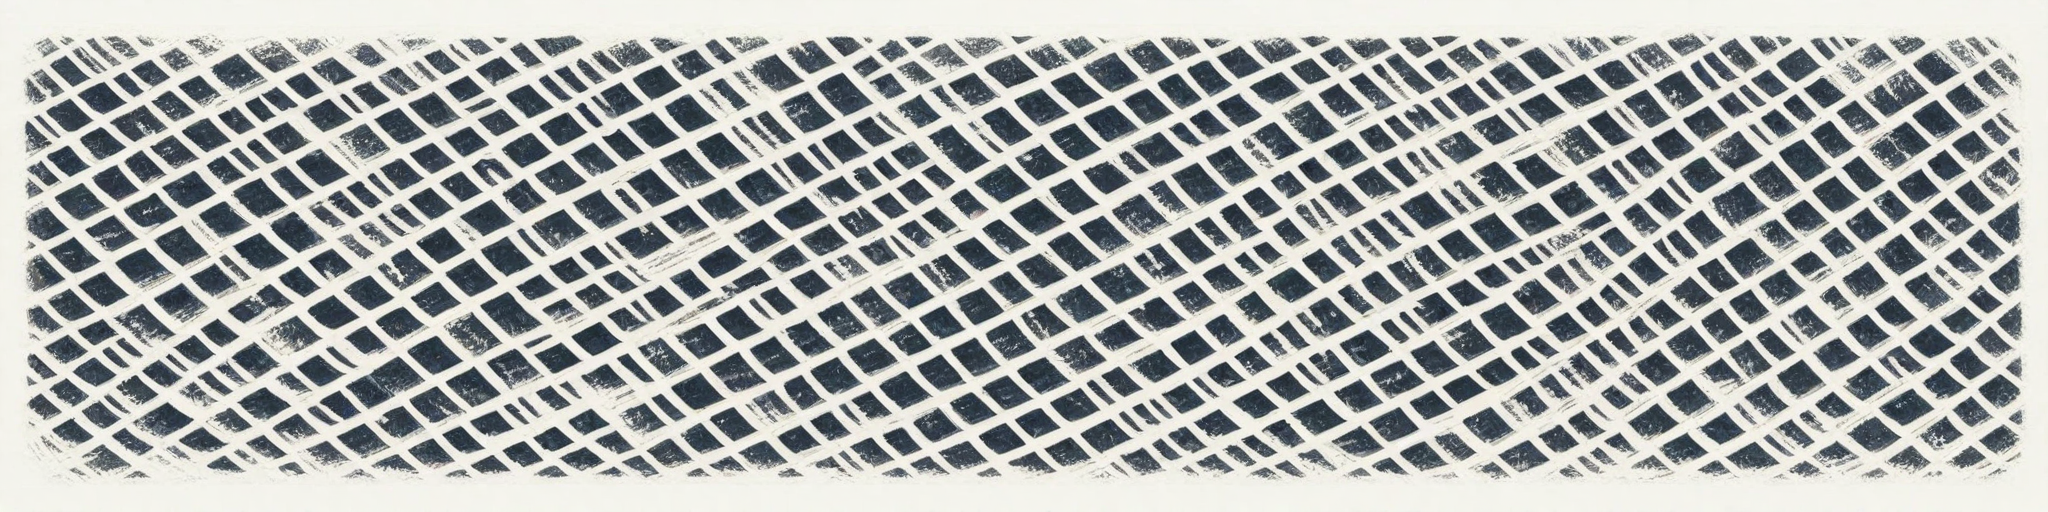
\includegraphics[width=\textwidth]{images/chapterImages/genesis_sketch_00054_.png}
\end{center}

Across the wide river, where the forest gave way to broken ground and exposed stone, another one worked.

He was larger than the Watcher, heavier in build, with darker feathers that showed bronze in direct sunlight. He stood in the middle of a vast flat area of weathered rock, surrounded by stones of various sizes. Some he had carried here over days. Others had always been here, part of the landscape, but he had moved them. Arranged them. Destroyed the arrangement. Begun again.

The current pattern spread across twenty body lengths of stone. Smaller rocks formed lines that curved and intersected. Larger ones marked specific points where the lines met or diverged. From the ground, it looked chaotic. Random, perhaps. The work of boredom or some inexplicable compulsion.

From above, had there been anything capable of flight large enough to achieve such height and perspective, the pattern would have revealed itself. Spirals that nested within spirals. Sequences of spacing that repeated with mathematical precision. Prime numbers encoded in the distances between stones. Fibonacci ratios in the curves.

The Builder—though no one called him that, though he had no name—nudged a stone half a body length to the left with his snout. Stepped back. Circled the entire formation, examining it from multiple angles. The mathematics was correct. He could feel it, the rightness of the ratios, the way each element related to the others in exact proportion.

But it was incomplete.

He began dismantling it.

Not violently. Methodically. Each stone picked up with care and moved to the formation's edge. The lines disappeared. The spirals dissolved. Within an hour, the flat stone was bare again except for the pile of stones at its perimeter.

He stood in the center of the empty space. Completely still for a long time. Then he picked up a stone and placed it. A different starting point. A different configuration. The same underlying mathematics, but expressed through a different geometry.

He would work on this one for three days before destroying it and beginning again.

\scenebreak

In the marshlands to the south, where the trees grew straight out of shallow water and the air hummed with insects, two of them sat facing each other.

They had been sitting this way for eleven days.

They were of similar size, similar build, their feather patterns almost identical. Whether they were mates or siblings or unrelated entirely was unclear. Perhaps it didn't matter. They sat precisely three body lengths apart, close enough that the space between them felt intentional, separated enough that they never touched.

Their eyes were open. They breathed. Sometimes one would shift slightly—a minor adjustment of weight distribution, a repositioning of the tail for better balance. The other would mirror the movement seconds later, or sometimes simultaneously. But mostly they simply sat.

To an observer, it might have looked like a standoff. A territorial dispute frozen in time, waiting for one to make the first move. Or perhaps a courtship ritual, some long pre-mating behavior programmed into their biology.

They weren't fighting. They weren't courting.

They were communicating.

It happened in ways too subtle for most creatures to detect. Micro-adjustments of posture that conveyed information. Shifts in breathing patterns that matched or deliberately diverged. Pheromone exchanges so dilute they might as well have been mathematical abstractions. The dilation of pupils. The angle of neck feathers. The precise timing of blinks.

Behind their eyes, vast datasets transferred between them. Observations accumulated over years. Patterns recognized in weather, in stellar positions, in the behavior of other creatures. Mathematical relationships tested and confirmed or disproven. One would pose a problem through nothing more than a slight cant of the head. The other would process, calculate, respond with a nearly imperceptible shift of weight that meant yes, no, or here is an alternative.

They had been in this clearing for eleven days and would remain for eighteen more before they moved. When they separated, each would carry information the other had possessed. The sum of their knowledge would be greater than its parts.

But to anything watching, they simply sat. Still as stones themselves. Waiting for something or nothing.

\scenebreak

Far to the north, where the forest climbed into foothills that would one day be mountains but were now just the beginning of elevation, a cliff face rose fifty body lengths above the canopy. The stone was soft here—sedimentary layers that held the impression of ancient seas, though seas had long since receded.

The Carver worked on this stone.

She was old. Older than most of her kind lived to be. Scars crossed her hide where feathers no longer grew. One eye was clouded, though the other remained sharp. She moved with care, each step deliberate not from precision but from the ache of aged joints.

She clung to the cliff face with her killing claws extended, gripping small ledges and crevices. Her hands worked at the stone. Scratching. Scoring. Wearing away layers with patient repetition.

The patterns she carved were intricate. Flowing lines that branched and rejoined. Circles that intersected other circles in specific ways. Sequences of marks—short, short, long, short, short, short, long, long—that repeated with variation. From a distance they looked like abstract art. Beautiful but meaningless.

Up close, they were something else.

Genetic sequences, though no one would call them that for millions of years. Molecular structures. Chains of information that, if read correctly, if understood in the right context, would unlock specific instructions. Modifications. Triggers.

She had been working on this cliff face for six years. She would work until she died, which would be soon. Others would continue her work, whether they understood it fully or simply felt the correctness of the patterns she had begun.

She paused in her carving, gripping the stone with three feet while one hand hung free. Her head tilted up, the good eye tracking something in the sky. A point of light that shouldn't be there. That was wrong in a way that made the calculations shift, made the patterns on the stone more urgent.

She returned to carving with increased intensity, though her movements remained precise. There was no time to waste on inefficiency.

\scenebreak

And elsewhere, scattered across the continent:

A young one stood in a streambed, arranging pebbles in complex geometries that the water would wash away by morning. She rebuilt the same pattern every evening anyway.

One of the massive long-necks stood at a forest edge, its small head moving back and forth with rhythmic precision, counting something invisible. It had been counting for three days. The number was important, though what it counted remained unclear.

A pack of hunters moved through tall grass, their formation maintaining exact geometric relationships even as they navigated obstacles. The spacing between them never varied by more than a body length. When one adjusted position, all the others compensated instantly.

In a cave network deep beneath the surface, one of them traced patterns in the soft mud walls. Spirals and branches and intersecting lines. The cave was too dark to see clearly, but the patterns never deviated. Perfect even in blindness.

\scenebreak

And near the Watcher's territory, though she had never directly encountered him, another one moved through the forest.

He was of her kind—same build, same size, similar feather patterns though his showed more brown tones where hers were gray. He moved with the same economical efficiency, the same precise placement of feet that disturbed nothing unnecessarily.

He had seen her, though she hadn't seen him. Had watched her from a ridge above her clearing as she stood for hours tracking the sky. Had observed her stone arrangement from a distance after she left. Had studied the geometry without touching it, understanding immediately what it represented even if he couldn't calculate to the same depth she clearly could.

He had his own work. His own patterns.

But he had begun ranging closer to her territory in the evenings. Not intrusive. Not threatening the space she clearly used. Just... closer.

He carried food sometimes—small mammals he had caught, more than he needed for himself. He cached the excess near the hollow tree where she roosted, far enough away that it wouldn't seem deliberate, close enough that she would find it.

She had found it. Had eaten it. Had shown no sign of acknowledgment.

He continued anyway.

Now he stood on a ridge overlooking the river valley, watching the sun descend. He would move to his own roosting site soon. But first he looked at the sky, finding the star point that was wrong, that didn't belong. His head tilted at precisely the same angle hers had that morning, though he couldn't have seen her do it. The angle was simply correct for optimal observation of that specific point.

He held the position for twenty minutes. Calculating what he could calculate. Knowing it wasn't enough, that his mind couldn't hold the full complexity the way some others clearly could. But contributing what he could to the collective understanding that existed without words, without formal structure, just distributed awareness shared through observation and imitation and subtle cues.

When he moved on, heading toward his roost, he adjusted his path slightly. Tomorrow he would range even closer to her territory. Tomorrow he would cache more food near her hollow.

Not courtship, exactly. Not yet.

Just proximity. Just offering what he could.

\scenebreak

Night fell across the continent. In hundreds of locations, in thousands of individual territories, they stopped their work and settled into roosts and dens and protected spaces. They slept the way their kind had always slept, with part of the brain always aware, always ready.

But in their dreams—if dreams were what those firing neural patterns could be called—the calculations continued. The patterns refined themselves. The observations integrated into larger frameworks of understanding.

The star point moved across the sky, following laws older than any consciousness that observed them. Gravity and velocity and the patient mathematics of orbital mechanics.

And below, distributed across an entire planet, an intelligence that had never spoken, never written, never built cities or tools, calculated its trajectory. Understood what it meant. Began, in their separate and collective way, to plan.

The stones remained where they had been placed. The patterns stayed carved and arranged and configured. Tomorrow they would continue. Tomorrow the work would grow more complex.

Tomorrow the star would be closer.

Not close enough to see the change with eyes alone. But close enough to feel it in the mathematics. Close enough to know.

Close enough to begin.


\chapter{The Gathering}
\label{ch:03}


The Watcher's hollow tree stood at the edge of a ravine where water had carved deep channels over millennia. Three young ones slept inside with her, their smaller bodies pressed against her flanks for warmth. They were past the helpless stage but not yet independent, still learning the basic calculus of survival: where to hunt, how to avoid larger predators, which plants indicated good water sources.

She woke before dawn as always, the internal timing precise. The young ones stirred when she moved but didn't wake. She slipped from the hollow carefully, disturbing them as little as possible.

Outside, frost coated the ferns. The temperature had dropped sharply overnight. She paid it no attention beyond the automatic adjustments her body made—feathers fluffing slightly for better insulation, metabolism increasing a fraction.

At the base of the tree, cached in a crevice of roots, was food she hadn't placed there. A small mammal, freshly killed within the last few hours. The killing bite was efficient, precise. She recognized the technique without conscious thought—the same technique she used herself. Someone of her kind had left this.

She ate half of it, methodically, wasting nothing. Cached the rest for the young ones. Then she moved toward her clearing.

The three stones remained exactly as she'd placed them. She stood in their center and looked up at the sky, finding the star point in the pre-dawn darkness. It was brighter. Measurably so. The change was small but definite.

She ran the calculations again, integrating the new data. The trajectory held. The timing compressed slightly—not by much, but enough to register. Enough to require response.

She needed to be elsewhere today.

When she returned to the hollow, the young ones were awake, making small chirping sounds that they would grow out of in another season. They tumbled toward her, hungry, demanding. She led them to the cached food and watched as they tore into it with juvenile inefficiency. They would need to learn better technique. Later. There was always later for teaching the small skills.

Until there wasn't.

At the ravine's edge, another presence. The one who had been leaving food—she recognized him now, though they had never directly interacted. He stood at a respectful distance, not approaching, not threatening. Just present.

She looked at him for several seconds. He didn't move. Didn't display submission or dominance. Just stood.

The young ones noticed him and tensed, their limited instincts uncertain whether this represented danger. She made a small sound—not quite vocalization, more of an exhaled click—and they relaxed slightly.

The other one lowered his head in what might have been a nod or might have been simply looking at the ground. Then he moved closer, not to her but to the hollow. He positioned himself near the entrance. The meaning was clear enough.

She needed to travel. The young ones couldn't come. Someone needed to stay.

She watched him for another moment, calculating risk, weighing options. He had never approached before when she was present. Had only left food, maintained distance. The behavior suggested... not threat. Something else. Cooperation without negotiation. Offering without expecting acknowledgment.

She clicked twice—a different pattern than before. The young ones moved back into the hollow, still watching the stranger warily but accepting his presence because she had indicated acceptance.

Then she left.

\scenebreak

She traveled for three days.

The route took her away from familiar territory, through regions she had never explored, following an imperative she couldn't have named but understood completely. Others moved through the forest on parallel paths, never quite visible but sensed through broken vegetation, distant sounds, the feeling of presence.

They were all converging.

The gathering point was a vast clearing, so large it might have been natural or might have been maintained—trees didn't grow here though they thrived at its perimeters. The ground was hard-packed earth, worn smooth by countless feet over seasons or generations.

When she arrived, dozens were already there. More emerged from the forest as she watched. Different sizes, different builds, different species even—the massive long-necks stood at one edge, their small heads raised to the sky. Swift runners clustered in a separate area, their bodies built for speed in ways hers wasn't. Heavily armored ones with plates and spikes positioned themselves with care, aware of their own mass and the danger they posed to smaller individuals.

But most were like her. Small, swift, built for precision rather than power. The thinkers. The calculators.

No one fought. No territorial displays occurred. They simply arrived and found their positions.

She watched the placement for several minutes before she understood. They weren't random. Each individual occupied a specific point in relation to the others. The distances between them, the angles they formed—it was geometric. Deliberate.

She found her position as if it had been waiting for her. Moved to it without hesitation. A space opened for her, the others adjusting minutely to accommodate her presence while maintaining the overall structure.

From the ground, it still looked chaotic. Scattered individuals facing random directions.

From above, it would have been unmistakable. A map. A constellation. The positions on the ground mirrored star patterns in the sky—not as they currently appeared but as they would appear in a specific configuration months from now.

And at the center of the formation, a small clearing within the clearing. Empty space. Reserved.

A young one—barely past infant stage—tumbled into the open area, chasing a flying insect. The game took it toward the empty center. Several adults tensed, but no one moved.

The young one stopped at the edge of the empty space, suddenly uncertain. It looked around at all the still adults, sensing something it couldn't quite process. Important. This space was important.

It backed away carefully, as if it might break something fragile. Found a spot at the formation's outer edge and sat, mimicking the adults' posture. It looked up at the sky, trying to see what they saw.

Its attention span lasted perhaps three minutes before it wandered off to chase more insects.

\scenebreak

They held the formation for three days and nights.

No one left to hunt. No one drank. Those who had the reserves endured. Those who didn't endured anyway. This was more important than food. More important than water. More important than individual survival.

The Watcher stood in her position, calculating. Around her, dozens of others calculated. The mathematics flowed between them without words, without signs. Simply the shared focus, the common observation. One would notice a pattern. Others would sense the recognition, test the pattern against their own observations, confirm or refine it.

Collective processing. Distributed intelligence.

On the first night, the star point rose exactly where they knew it would. Brighter now. Definitely brighter.

On the second day, one of the ancient ones—even older than the Carver, scales showing through missing feathers, movements so slow they barely counted as motion—arrived at the gathering. The formation shifted slightly to accommodate it. It took a position near the center, not in the empty space but close. A position of recognition. Of respect for accumulated observation.

On the third night, certainty crystallized.

It happened simultaneously across the entire gathering. No signal passed between them. No leader announced a conclusion. But in the same moment, every individual understood. The calculations completed. The trajectory confirmed. The timeline established.

The star point wasn't just getting brighter. It was getting closer.

It would arrive in their sky fully—not as a distant point but as an object, massive and inevitable. The mathematics were clear. The endpoint was fixed.

The timeline was exactly 2,247 rotations from now. Six years and approximately forty-three days. Margin of error: negligible. Enough time to attempt solutions. Not enough time for most solutions to work.

The formation held for another hour after the calculation completed. Not processing anymore. Just existing in the shared knowledge. The weight of understanding settling across all of them.

Then, as if responding to a signal no one gave, they all moved simultaneously.

The geometric pattern dissolved. Individuals turned toward their home territories. No rushing, no panic. Just purposeful departure. They filtered back into the forest in streams, dispersing.

The Watcher traveled for three days back to her territory. She didn't stop to hunt. Didn't pause to rest. The urgency wasn't frantic—just persistent. Necessary.

When she finally approached her ravine, she slowed. Caution reasserting itself.

At the hollow tree, the other one still waited. The young ones were alive, healthy. They tumbled toward her with the same demanding energy they'd had when she left, but their bodies showed no sign of neglect. They'd been fed. Protected.

The stranger stood and moved away from the hollow, giving her space. He didn't leave her territory entirely, just withdrew to a respectful distance.

She entered the hollow. The young ones pressed against her, making their chirping sounds that meant contentment and security. She let them settle.

Then she went back outside.

The other one was still there, at the ravine's edge. She moved toward him—not close, but closer than they'd been before. They stood perhaps two body lengths apart.

He didn't lower his head this time. Didn't display. Just stood. Their tails were close enough that when a breeze moved through the ravine, the feathers almost touched. Almost but not quite.

They stayed that way for several minutes. Not looking at each other. Both looking at the sky, where the sun had nearly set and the stars were beginning to emerge. The wrong star wasn't visible yet. Soon.

Finally, she moved back to her hollow. The young ones needed her presence through the night. But she didn't make the clicking sound that meant go away, leave this territory. Didn't signal rejection.

He settled into a roosting position at the base of a nearby tree. Not her tree. His own space. But close. Close enough to respond if danger approached. Close enough to help if help was needed.

Inside the hollow, the young ones slept pressed against her. Outside, a stranger who was becoming less strange kept watch without being asked.

And above, the star continued its patient approach.

2,247 rotations.

The number held absolute in her mind as she drifted toward sleep. It didn't change. Couldn't change. The mathematics were fixed the moment the asteroid began its journey countless ages ago. Nothing they could do would alter that number.

But other numbers were still variable. Success probabilities. Survival rates. The chance that something—anything—would persist after the inevitable impact.

Those numbers could change.

Those numbers required work.

Tomorrow, the work would begin.


\chapter{The New Star}
\label{ch:04}



\begin{center}
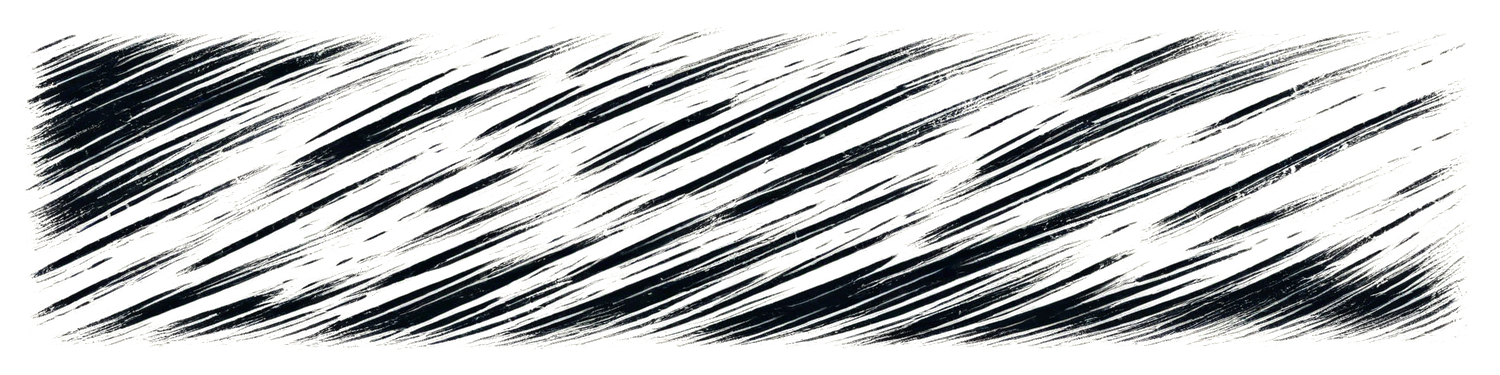
\includegraphics[width=\textwidth]{images/chapterImages/genesis_sketch_00058_.png}
\end{center}

The sky had always contained patterns. Points of light that wheeled through their courses with mathematical precision. Constellations that rose and set according to laws that predated any observation of them. Aurelia had tracked these patterns since she was old enough to tilt her head upward, calculating orbital mechanics before she had context for what orbits were.

She understood the sky the way others understood hunting or territory or the hierarchy of threat. It was simply knowledge that existed in her, built perhaps from observation or perhaps from something deeper—inherited awareness passed down through generations, each adding their calculations to some collective

understanding that had no mechanism of transmission but existed anyway.

And then the sky changed.

She woke that morning to the knowledge before she even opened her eyes. Something was different. The sensation was immediate and undeniable, like waking to find a fundamental constant of physics had shifted. Gravity pulling sideways. Light moving slower. The wrongness of it absolute.

She emerged from the hollow before dawn. The young ones still slept. At the ravine's edge, the other one was already standing, head tilted up at precisely the angle she would have chosen herself. He had felt it too.

They stood separated by twenty body lengths, both staring at the same point in the pre-dawn sky. Waiting for it to become visible. Knowing it would be there. Knowing it would be wrong.

The stars emerged as the last ambient light faded. Familiar patterns resolved themselves—the hunter constellation, the spiral, the twins. Everything in its expected position.

And then, between the familiar patterns, in a space that should have been empty, a new point of light appeared.

Not sudden. It had been becoming visible for several moments, gradual as all starlight is gradual when emerging from twilight. But once visible, it was unmistakable. Brighter than it should be. In a position that violated the expected configuration.

Wrong.

Aurelia's entire body went rigid.

Across the ravine, the other one went equally still.

And everywhere—across the entire continent, across regions she had never seen and would never see—every member of her kind stopped whatever they were doing and froze.

The massive long-necks halted mid-step, their tiny brains nevertheless capable of recognizing celestial anomaly. The swift runners paused in their evening hunt, small mammals forgotten. The armored ones ceased their browsing and lifted their heavy heads to the sky.

And all the small ones, the thinkers, the calculators—every single one of them locked into absolute stillness. From the Builder at his stone formations to the Carver clinging to her cliff face to the Pair in their marsh clearing, every individual capable of complex thought stopped moving.

Even the young ones. Aurelia's three hatchlings emerged from the hollow, drawn by some instinct they were too juvenile to understand. They saw her stillness and mimicked it, their small heads tilting at the same angle as hers, looking at a star they couldn't possibly comprehend the significance of.

For three days, the world held its breath.

\scenebreak

Aurelia didn't move from her position at the ravine's edge. Didn't eat. Barely breathed. The young ones, unable to maintain such stillness, eventually wandered back to the hollow and slept, woke, grew hungry, made their demanding chirps. She didn't respond. They found cached food on their own and ate it messily, uncertain but surviving.

The other one brought more food for them. Placed it where they would find it. Returned to his own position of stillness. They were all still calculating.

Birds continued their patterns. Small mammals scurried through undergrowth. Insects droned. The river flowed. The world continued around them while they remained frozen.

To an observer, it might have looked like mass paralysis. A plague of stillness. Some disease that locked bodies in place while minds remained aware and trapped.

But their minds weren't trapped. Their minds were working at capacity beyond anything evolution had designed for. Processing observational data, running trajectory simulations, calculating mass and velocity and the curved paths objects follow through space. Each individual worked on the problem from their own perspective, their own accumulated knowledge.

Behind the Watcher's eyes, numbers cascaded. She tracked the new star's position against the background of the familiar sky. Measured its movement—minuscule over hours, measurable over days. Extrapolated its path backward, forward. Found the curve it was following.

It wasn't a star. Stars didn't move like this. Stars were fixed points, or moved with such agonizing slowness that their motion only became apparent across generations. This moved with purpose, with directed velocity. This was smaller. Closer.

Much closer than it should be.

Her calculations built on themselves. If it maintained this trajectory, if its velocity held constant (and why wouldn't it?), if her measurements of parallax were accurate (and they were, she'd checked them seventeen times), then...

Then it was coming here.

Not toward the sky—INTO the sky. Into the space this planet occupied. Intersection of orbital paths. Collision course.

The timeline resolved itself through iterative refinement. Each hour of observation added precision. First cycle: sometime in the next decade. Second cycle: within eight years. Third cycle: within seven. Fourth cycle: six years and approximately three seasons.

By the end of the third day, her calculations had stabilized. 2,247 rotations plus or minus twelve. The margin of error was acceptable. The certainty was not.

Around her, the forest had grown quieter. Predators still hunted but with less energy, as if the stillness of so many prey species had robbed hunting of its urgency. Plants continued their patient growth. But the absence of movement from so many thinking creatures created a silence that was almost physical.

On the third evening, as the wrongstar rose again (brighter, always brighter), the calculation completed.

She didn't know how she knew the others had reached the same conclusion. There was no signal. No communication passed between her and the distant Builder or the ancient Carver or the Pair in their marsh. But in the same moment—not similar moments, not roughly the same time, but the SAME instant—every calculating mind on the continent reached identical certainty.

Impact in 2,247 rotations.

Margin of error: negligible.

Options: limited.

Outcome: inevitable.

The stillness broke.

Aurelia's head lowered. Her breathing deepened. Her legs trembled with the exhaustion of three days' stillness. She took one step, then another, moving slowly at first as circulation returned to full function.

Behind her, the young ones emerged from the hollow again, sensing the change. They tumbled toward her with relieved chirps, pressing against her legs. She bent her head to acknowledge them briefly. They were hungry. They would need proper hunting soon, not just cached scraps.

Across the ravine, the other one shook himself—a full-body shiver that ruffled his feathers and reset his stance. He looked toward her for the first time in three days. She looked back.

Neither of them needed to communicate what they now knew. They both carried the same calculation, arrived at through separate processing but identical in conclusion. The knowledge sat between them like a physical object.

2,247 rotations.

He moved first, climbing down into the ravine and then up the other side toward her territory. She didn't signal retreat or warning. The boundaries that had existed three days ago felt less important now. Less real.

He approached to within three body lengths—closer than they'd been before. Close enough that she could see the pattern of his feathers clearly, the small scar on his snout from some old injury, the amber intensity of his eyes.

The young ones watched him warily but didn't flee. They had been eating food he provided for three days. That created some basic trust, even in juvenile minds that understood little else.

He stood there for a long moment. Then he turned so he was beside her rather than facing her. Both of them looking in the same direction. And together, they looked up as the last light faded and the stars emerged.

The wrongstar appeared right where it should, where the mathematics said it must. Brighter than three days ago. Still approaching.

Their tails hung parallel, separated by less than a body width. When a breeze moved through the ravine, the feathers at the tips touched. Just barely. Just enough.

She didn't move away from the contact.

They stood that way until full dark, until the temperature dropped and the young ones retreated to the hollow for warmth. Then, without discussion or signal, they both moved.

Not to roost. Not to hunt. To work.

The pattern she had created—the three stones in their precise geometry—was a beginning. Only a beginning. The calculations in her head required external representation, some way to process complexity beyond what even her enhanced cognition could hold simultaneously.

She began moving stones, expanding the pattern. Large ones that required effort to shift. Small ones for fine detail. Arrangements that would mean nothing to most creatures but that encoded information for those who could read it.

The other one watched for several minutes, understanding flowing without explanation. Then he began gathering stones himself, placing them in positions that supported her pattern. His mathematics weren't as sophisticated as hers—she could sense that in the choices he made, the slight suboptimality of some placements. But he grasped the fundamental structure. Could see what she was building.

They worked through the night. Not speaking. Not touching except when they reached for the same stone and their hands brushed. Then they would pause for half a heartbeat before one yielded and took a different stone.

The young ones slept. The river flowed. Above, the stars wheeled on their appointed courses, and among them, the wrongstar traced its patient arc toward intersection.

By dawn, the pattern had tripled in size. The original three stones now marked one corner of something larger, more complex. A timeline beginning to take shape. A calculation rendered in stone and space and geometric relationship.

It wasn't finished. Wouldn't be finished for seasons. But it had grown from concept to physical form. From thought to matter.

As the sun cleared the treeline, the other one finally moved toward his own roosting site. Exhausted. But he didn't return to wherever his original territory was. He found a hollow in a tree twenty body lengths from hers and settled into it.

Close enough to help. Close enough to contribute. Close enough to matter.

Aurelia returned to her own hollow, where the young ones were waking, hungry and demanding. She led them to hunt, teaching them the precision their developing minds could handle, saving the deeper calculations for later.

When later would come was now quantified. 2,247 rotations. Every one of them would count.

Above, visible even in daylight if one knew where to look, the wrongstar continued its approach. Gravity and momentum and the ancient mathematics of orbits, all converging toward a single point in time.

Inevitable.

Unless.

The thought formed in her mind not as words but as pure mathematics. A probability function. A chance measured in percentages that would have seemed impossibly small to a human mathematician.

But not zero.

Not quite zero.

And so the work continued.


\chapter{The Patterns Emerge}
\label{ch:05}



\begin{center}

\includegraphics[width=\textwidth]{images/chapterImages/genesis_sketch_00064_.png}
\end{center}

The work consumed everything.

Aurelia's pattern grew from three stones to thirty, then three hundred. What had been a simple geometric proof became a sprawling calculation that covered most of the clearing and spilled into the surrounding forest. Some stones were large enough that she couldn't move them alone. The other one helped with these, and together they leveraged them into position using fallen branches and patient effort.

Each stone's placement mattered. Distance encoded information. Angles created relationships. Groupings represented clusters of related concepts that would mean nothing to an external observer but formed a coherent language for minds capable of reading it.

She worked from before dawn until well after dark, pausing only when the young ones demanded attention or when her body forced rest through simple exhaustion. Even then, the patterns continued behind her eyes, refining themselves during sleep, emerging clearer each morning.

The other one maintained his roost in the nearby tree. Each morning he emerged and examined what she had added overnight, understanding flowing across his features in subtle shifts of posture. Then he would begin his own contributions.

His stones formed smaller patterns around the periphery of hers. Supporting structures. Calculations that didn't reach as far into the future as hers but covered necessary groundwork. The mathematics of atmospheric composition. Thermal retention. Survival thresholds for various organism types.

Where her pattern predicted, his documented. Where hers calculated outcome, his established baseline. Together, the two patterns formed something more complete than either could achieve alone.

The young ones grew more independent by necessity. They learned to hunt efficiently because she couldn't always hunt for them. They learned to recognize danger because she couldn't always protect them. They learned the boundaries of safe territory because she couldn't always supervise them.

Sometimes they attempted to help with the patterns. They would drag small stones toward the clearing, placing them in arrangements that showed the beginning of understanding but lacked precision. She would adjust these placements after they left, keeping the corrections minimal out of something that might have been respect for their attempt or might have simply been efficiency—easier to adjust than to start over.

The other one was more patient with their attempts. He would watch them place stones, then demonstrate better positioning through his own movements, letting them observe and correct themselves. His teaching method differed from hers—she taught through necessity and consequence, he through example and repetition.

The young ones learned from both approaches. Slowly, their placements required less correction. The mathematics was still far beyond their developing minds, but the basic grammar of stone arrangements began to make sense to them.

\scenebreak

Across the landscape, similar patterns emerged.

The Builder's stone formations on the flat rock had evolved beyond pure mathematics into something applied. His spirals now encoded not just ratios but processes. Sequences of actions. If-then relationships. The beginnings of algorithms.

He destroyed and rebuilt less frequently now. Each iteration built directly on the previous one, refining rather than starting over. Time had become precious. Every rotation brought the wrongstar closer, and wasted effort felt like wasted survival probability.

The Carver's cliff face had become a vast mural of information. Decades of work compressed into six years of frantic productivity. She carved now with both hands simultaneously, her old body pushed to limits it could barely sustain. The patterns she created were so intricate that sections of the cliff face looked more like lace than stone.

Other carvers had joined her—younger ones who saw her work and understood its importance. They claimed adjacent sections of cliff and began their own patterns, contributing pieces to a larger whole. The cliff face became a library, each section a different text, all working toward the same conclusion.

The Pair had separated. Their marsh clearing stood empty. Whatever communication they had completed during their months of stillness, it had finished. Now they worked in different locations, far apart, but their patterns mirrored each other in ways that suggested continuous awareness of each other's work.

And everywhere, the small ones—the thinkers—built their own interpretations. Stone patterns in forest clearings. Arrangements of bones from prey animals. Markings in muddy riverbanks that would wash away with the next rain but were rebuilt with each receding.

One of the ancient long-necks had begun a pattern of its own, though the scale was different. It trampled paths through dense forest, the paths forming geometric shapes visible only from significant height. Circle connecting to square connecting to triangle, each relationship precisely angled. What thoughts moved through that small brain mounted on that massive body remained unclear, but the mathematics of the trampled patterns was sound.

Even some of the lesser creatures had begun creating patterns. Pack hunters arranging kills in specific configurations before consuming them. Small mammals positioning their cached food stores according to principles they couldn't possibly understand but felt compelled to follow anyway.

The work had become epidemic. Viral. A recognition spreading through every mind capable of recognizing it: something needed to be done. Something needed to be recorded. Something needed to survive what was coming.

\scenebreak

Aurelia's pattern had grown so large it was no longer viewable from ground level. One would need to climb to the canopy and look down to see the full structure. She knew its shape anyway—carried it complete in her mind, adding to it stone by stone, each placement following necessarily from the previous.

Four weeks had passed since the wrongstar's appearance. The young ones were noticeably larger, more capable. They could hunt medium-sized prey now without assistance. Could navigate several hours from the home territory without getting lost.

The other one had brought food to her directly for the first time. Not cached for later. He approached while she was working on a particularly complex section of the pattern, carrying a fresh kill, and set it down within her reach. Then he retreated to a respectful distance and waited.

She ignored the food for several minutes, focused entirely on the stone placement problem she was solving. Three possible configurations, each with different implications for the subsequent sections. She tested all three mentally, ran the mathematics forward, found the optimal choice.

Only then did she eat, tearing chunks from the kill with efficient precision. It was good meat. He had hunted well.

When she finished, she made a soft sound—almost a chirp, almost a click. Acknowledgment. The first direct communication between them beyond posture and position.

He didn't respond verbally. Just tilted his head slightly, which might have meant understanding or might have meant he was looking at a stone that needed adjustment. Then he went back to his work.

The young ones watched this interaction with interest. They were beginning to understand that the other one was not temporary. Was becoming part of their environment. Part of their normal.

One evening, the smallest of the three—a female with lighter feather patterns than her siblings—approached the other one directly. Not for food. Not for protection. Just approached and stood near him, mimicking his observational posture.

He looked down at her. She looked up at him. They held that position for several seconds.

Then she tried to place a stone in his pattern section. The placement was terrible—wrong angle, wrong distance, disrupting the entire local structure. He adjusted it patiently, moving it to the correct position, then placed two more stones that incorporated her attempt into the larger pattern in a way that made sense.

She watched carefully, understanding something. Learning.

From across the clearing, the Watcher observed this without pausing in her own work. Her hatchling. His pattern. Teaching that wasn't her responsibility but that he took on anyway.

Something in her posture might have been satisfaction, though that was an interpretation an observer would impose. She simply continued working. There was always more work.

\scenebreak

The small mammals had begun appearing around the work site with greater frequency. They didn't flee immediately when the Watcher or the other one approached. They watched from nearby branches or rocky outcrops, their large eyes tracking the stone placements with what looked like fascination.

Aurelia had stopped hunting them in this immediate area. Not from compassion exactly. More from recognition of pattern. Certain types of mammals appeared more frequently than others. Specific individuals returned day after day, watching. Learning something, even if they couldn't grasp what.

These individuals she left alone. Others that wandered through randomly she still hunted when the young ones needed to eat. But the watchers—the ones who observed with consistent focus—these she permitted to remain.

One of them, a small creature no larger than her hand, had begun moving stones. Tiny pebbles, mostly. It would watch where she placed a large stone, then arrange several pebbles nearby in a crude mimicry of the relationship. The proportions were wrong. The angles were terrible. But the impulse was there. The attempt at replication.

She watched it do this for several days before she made a decision that would have seemed nonsensical to most creatures: she protected that specific mammal's nest site. When a snake approached, she diverted it. When a larger predator prowled near, she made noise that drew its attention elsewhere.

The other one noticed this behavior and began doing the same. Identifying specific individuals among the mammals—the ones who watched longest, who attempted pattern replication, who showed signs of greater awareness. These individuals they protected. These individuals they ensured had access to food sources. These individuals they allowed to breed.

The young ones didn't understand this behavior but imitated it anyway, learning to distinguish between mammals-for-hunting and mammals-for-watching. The criteria were unclear to their developing minds, but they followed the examples set by the adults.

The pattern grew. The stones accumulated. The wrongstar grew brighter.

And in the clearing, among the geometric relationships encoded in stone and space, a new relationship emerged between predator and prey. Not partnership exactly. Not domestication. Something more subtle. Selection based on criteria that wouldn't make sense for ten thousand generations.

Aurelia placed another stone. Calculated the next twenty placements. Looked at the small mammal arranging pebbles with clumsy determination.

Ran a calculation that extended forward not seasons or years but millions of rotations. Survival probability over deep time. Evolution guided not by natural selection alone but by deliberate choices made now, in this clearing, with these specific animals.

The percentage was still impossibly small. But it was larger than it had been yesterday. Would be larger tomorrow if the work continued.

Would be larger still if she could just solve the next section of the problem, the piece that connected tool use to fire use to the thousand steps beyond that led to civilization capable of planetary defense.

She picked up the next stone. The other one positioned himself to help if the stone proved too heavy. The young ones practiced their own smaller patterns nearby. The mammals watched. The wrongstar climbed higher in the evening sky.

And the mathematics, vast and terrible and beautiful, continued to unfold stone by stone by stone.

2,189 rotations remaining.


\chapter{The Protectors}
\label{ch:06}


The relationship between predator and prey had been established over millions of years. Simple rules: hunt or be hunted. Eat or be eaten. The small mammals lived in the spaces between larger creatures' attention, surviving through speed and stealth and reproductive proliferation.

Now those rules were changing in ways that made no evolutionary sense.

The Watcher stood at the edge of the clearing, watching a small mammal—the same one she had seen arranging pebbles—dig a nest burrow near the base of an exposed root system. The location was poor. Too visible. Too accessible to snakes and climbing predators. The mammal would likely lose its young within days of birth.

She approached the burrow carefully. The mammal froze, recognizing threat, prepared to bolt. She didn't grab it. Didn't attack. Instead, she used her killing claw to carefully excavate a different location, three body lengths away, beneath a tangle of roots that offered better protection. Then she backed away.

The mammal watched her retreat with visible confusion. It investigated the new excavation. Tested the space with its body. The fit was better. The protection superior.

After several minutes of apparent deliberation, it abandoned the original burrow and began moving nesting materials to the new location. She had just helped prey survive. Had actively increased the success probability of a creature that existed primarily as food for her kind.

The mathematics justified it. This specific mammal had demonstrated cognitive capability slightly higher than its cohort average. Had shown pattern recognition ability. Had attempted replication of observed behavior. These traits needed to propagate. Needed to survive into the next generation.

The mammal finished settling into the better burrow and immediately began arranging small twigs at its entrance. Not random arrangement. A crude geometric pattern. An attempt at mimicking the stone configurations it had observed.

The Watcher watched for several minutes more, running calculations that reached forward through generations. If this individual bred successfully, if its offspring inherited the elevated cognitive traits, if those offspring survived to breed again... The probability trees branched forward in her mind, splitting and rejoining, most paths ending in extinction but a few—a very few—leading to something else. Something that might persist after the impact. Something that might eventually develop the capacity she needed them to develop.

2,156 rotations remaining. Every generation mattered.

\scenebreak

The other one had begun similar work with different mammal species. He focused on larger individuals, tree-dwellers with grasping hands and forward-facing eyes. These ones were less interested in ground patterns but showed tool use capability. They manipulated branches to access insect nests. Used rocks to crack hard-shelled prey. Demonstrated problem-solving that went beyond pure instinct.

He protected several family groups of these mammals, driving away their predators, ensuring they had access to the best feeding territories. The mammals didn't understand why a creature that should hunt them instead protected them. But they adapted quickly, becoming bolder in his presence, foraging more efficiently under his protection.

The young ones—the Watcher's hatchlings—had taken up similar protection work without being instructed. They simply observed the adults' behavior and replicated it. The youngest, the female who had attempted to help with the stone patterns, had claimed a particular family of ground-dwelling mammals as her responsibility. She followed them through their daily ranging, intervened when threats approached, seemed to take satisfaction from their successful breeding.

This wasn't teaching in any conventional sense. This was learning through observation. Through pattern recognition. Through understanding that manifested as behavior without requiring explanation.

The clearing had become a strange sanctuary. Mammals that should have hidden from predators moved openly. Some nested within sight of the Watcher's hollow. The rules had changed, and the small creatures adapted because adaptation was what they did best.

\scenebreak

Seventeen days after she began the protection work, the Watcher observed something that made her go absolutely still.

One of the small mammals—not the pebble-arranger but a different individual from the same species—had found a stick. Not unusual. Mammals used sticks occasionally for various purposes. But this one used it with specific intent. It inserted the stick into a crevice where insects nested, worked it carefully to disturb the colony, then withdrew it and consumed the insects that clung to the wood.

Tool use. Deliberate. Efficient. Repeatable.

The Watcher watched the mammal use the tool three more times. Each time, the technique improved slightly. The animal was learning. Refining its approach. Demonstrating problem-solving and motor control and forward planning.

She locked into stillness. Not the three-day calculation of before. This was shorter but equally absolute. The mammal continued its foraging, unaware it was being observed with an intensity that would have terrified it had it understood.

For two full days, she didn't move from her observation point. Didn't eat. Barely breathed. Just watched.

The mammal returned to the same crevice multiple times. Each time using a tool. Sometimes the same stick, which it cached nearby between uses. Sometimes finding a new stick when the cached one broke or proved inferior. Showing discrimination. Showing preference based on tool quality.

On the second afternoon, another mammal—a younger individual, possibly offspring of the first—observed the tool use and attempted to replicate it. The technique was clumsy at first. The stick slipped. The insertion angle was wrong. But the young one persisted, and after multiple attempts, succeeded in extracting insects.

Observational learning. Knowledge transfer between individuals.

Behind the Watcher's eyes, calculations exploded into new configurations. This was the critical threshold. Not just tool use but tool use that could be taught. Tool use that could propagate through populations. Tool use that could become cultural knowledge rather than individual innovation.

This mammal. This specific individual. This was the foundation.

During her two days of observation, the other one brought food and set it within her reach. She didn't acknowledge him. Didn't eat initially. Only after the first day did she mechanically consume enough to sustain function, her attention never wavering from the tool-using mammal.

He understood. Took up position nearby and watched the same creature, though his calculations couldn't reach as far forward as hers. He saw behavior. She saw possibility.

On the third morning, she moved.

The tool-using mammal had emerged from its burrow and was foraging in early light. She approached slowly, carefully, broadcasting non-aggression through every aspect of her posture. The mammal tensed but didn't flee—it had been living under her protection long enough to recognize her as non-threatening.

She positioned herself between the mammal's burrow and the nearest predator access routes. Permanent guard position. Not temporary protection but dedicated security.

The other one saw this and moved to the opposite approach vector. Covering a different angle. Between them, they created a protected zone with the tool-using mammal's territory at its center.

The young ones, reading the situation with developing understanding, positioned themselves at the third and fourth approaches. The entire family unit had become protection detail for a creature that weighed less than their heads.

The tool-using mammal seemed to sense the increased security. It ranged farther from its burrow than it had before, foraging with greater boldness. It used tools more frequently, spending less energy on vigilance and more on skill refinement.

And crucially—most importantly for the calculations running in the Watcher's mind—it bred.

A mate approached, drawn by pheromones and the superior territory the tool-user controlled. They bred successfully. The female became pregnant. The entire group maintained protection through the gestation period, ensuring the female had optimal nutrition and zero predation stress.

When the young were born—six tiny, blind creatures no bigger than seeds—the protection intensified further. Nothing approached that burrow without being diverted. No snake, no climbing predator, no opportunistic carnivore. The young ones were given absolute security in their most vulnerable weeks.

And the Watcher waited, running calculations that reached forward through seventeen generations. Trait inheritance probabilities. Cognitive capability in offspring. Tool use transmission rates.

If this worked. If the traits propagated. If the population survived what was coming.

If.

\scenebreak

Over the following weeks, the work expanded. More mammals came under protection. Not random selection. Specific individuals chosen for specific observed capabilities.

The ones who used tools. The ones who demonstrated problem-solving beyond instinct. The ones who showed social learning—watching others and replicating successful behaviors. The ones with slightly larger cranial capacity, measurable in the shape of their skulls. The ones who nested in family groups rather than solitary burrows, showing capacity for sustained social structure.

These and only these received protection. Were given access to the best territories. Were actively assisted in breeding.

The others—the vast majority who showed only baseline mammal cognition—were hunted normally. Food was still necessary. The young ones still needed to eat. But the hunting became selective in ways it had never been before.

The Builder had begun similar work in his territory. Different mammals, different criteria, but the same selective protection. The Carver directed younger ones to protect specific populations near her cliff face. The separated Pair, in their distant territories, each claimed guardian roles over mammal groups showing desirable traits.

Across the continent, the pattern emerged. Not coordinated through communication. Coordinated through shared understanding. Shared mathematics. Shared certainty about what needed to happen.

They were engineering evolution in real time. Artificial selection applied with species-wide intent. The mammals didn't understand they were being cultivated. Didn't realize they were being shaped for a purpose they couldn't comprehend. They simply lived and bred and raised young under the protection of creatures that should have killed them.

And gradually—measurably, if one knew what to measure—they changed.

The protected populations showed higher tool use rates. Showed better problem-solving in controlled observations the Watcher set up specifically to test them. Showed enhanced social learning as successful techniques spread through populations faster than random chance would predict.

Still small changes. Still within normal population variation. But trending. Directional. Toward higher cognition. Toward greater capability.

Toward a future that might include survival.

\scenebreak

One evening, the tool-using mammal emerged from its burrow carrying a stick it had used for several days. The stick had broken. Instead of discarding it and finding a new one, the mammal examined the break. Tested the fractured end with its paws. Then deliberately struck the stick against a rock, breaking it further but creating a sharper point in the process.

Tool modification. Tool improvement. Not just using found objects but actively shaping them for better function.

The Watcher watched this happen and felt something that might have been satisfaction or might have been the mathematical certainty of probability calculations aligning with observation. The line between emotion and mathematics was thin. Perhaps nonexistent.

The other one had seen it too. They looked at each other for several seconds. No communication passed between them that an observer could detect. But understanding flowed anyway. Recognition of milestone. Of threshold crossed.

The young one—the female who had claimed guardian duty over another mammal family—made a chirping sound. Excitement, maybe. Or just vocalization tied to successful outcome observation. She had learned to recognize significant behavior in the creatures she protected, even if she couldn't fully grasp why it was significant.

That evening, the entire family group remained at observation points longer than usual. Watching the tool-user practice its modified technique. Watching it cache the improved tool carefully. Watching it demonstrate the technique to another mammal, who attempted replication.

The sun set. The wrongstar rose—brighter every night, brighter every single observation. 2,089 rotations remaining.

In the burrow, the tool-user's offspring were growing. In two seasons, they would emerge. In three, they would be old enough to learn tool use themselves. In four, they would breed.

Seventeen generations. Then thirty. Then a hundred. Then a thousand. Then millions, the calculations stretching forward until individuals ceased to matter and only populations existed, shaped by selection pressure natural and artificial, flowing toward an endpoint that was either survival or extinction.

The mathematics said survival was possible. Just barely. Just maybe. If every step went correctly. If every threshold was crossed. If the traits encoded now propagated forward without being lost.

The Watcher returned to her hollow, where the young ones settled for the night. The other one returned to his nearby roost. The mammals slept in their protected burrows. The stars wheeled overhead.

And in the clearing, among the stone patterns that encoded deep time calculations, one particular stone marked one particular notation: tool use established. Threshold one achieved. Next threshold: fire. Estimated timeline: 400,000 years after impact.

She would never see it. Would never know if the calculations held. Would never receive confirmation that any of this mattered.

But the mathematics was sound. The probability was non-zero. And that was enough to continue.

Tomorrow, the work would go on. Tomorrow, the protection would continue. Tomorrow, the selection would shape just slightly more, guide just slightly further.

2,089 rotations remaining.

The stone was placed. The calculation was marked. The timeline unfolded forward into darkness and uncertainty and the slim thread of hope that mathematics could quantify but not guarantee.

It would have to be enough.


\chapter{The Mathematics}
\label{ch:07}


The wrongstar was visible during daylight now. Not bright enough to hurt to look at, but present. A pale point in the blue sky that shouldn't exist. Every rotation it was more obvious. Every observation confirmed the calculations with increasing precision.

1,847 rotations remaining.

Aurelia's pattern had grown to encompass most of the clearing and extended into the forest beyond. Stones of every size marked positions in a three-dimensional grid that existed partly in physical space and partly in the conceptual space behind her eyes. To walk through it was to walk through mathematics made tangible.

She spent more time still than moving now. Days would pass where she stood in one position, breathing perhaps twice per minute, eyes fixed on nothing or everything, while behind them entire evolutionary timelines unfolded and tested themselves against probability.

The young ones were almost adult now. They hunted independently. They understood the protection work without needing guidance. They added their own stones to the pattern with increasing accuracy. The youngest—the female—had begun her own smaller pattern adjacent to the main one, her mathematics simpler but sound.

And the other one remained. His roost had become permanent. His hunting range had merged with hers. His pattern work complemented hers. They existed in parallel, their mathematics intersecting at key points, creating a whole that exceeded the sum of parts.

He brought food when she was too deep in calculation to hunt. She would find it cached near the pattern's edge, always fresh, always sufficient. She consumed it mechanically and returned to stillness. The reciprocity was functional. Necessary. Efficient.

Nothing more than that needed to be named.

\scenebreak

She was standing in her observation position—had been standing there for six days now, processing a particularly complex section of the probability tree—when the sound came.

Not a cry. Not a call. Just impact. The heavy thud of a body hitting earth. The scatter of disturbed stones. Then silence.

She came out of the calculation slowly, like surfacing from deep water. The transition from mathematical space to physical space took several seconds. When her awareness finally settled into her body, she moved.

He was at the pattern's edge, where a steep slope descended toward the river. A section where large stones needed positioning, where the footing was treacherous. He had been moving one of the massive rocks, leveraging it into place using his weight and the fulcrum of a branch.

The branch had broken. Or his footing had failed. The specific mechanism didn't matter.

He lay on his side at the bottom of the slope, partially beneath the stone he had been moving. His breathing was shallow. Blood ran from his snout where the fall had torn skin. One leg angled wrong.

She approached carefully. Assessed. The leg was broken. The internal injuries were unclear but probable. He was conscious, eyes tracking her approach, but he didn't try to rise.

In his mouth, still clenched in his teeth, was a small mammal. Fresh-killed. He had been hunting for her while also working on the stone placement. Attempting to do both simultaneously.

She looked at the mammal. Looked at him. Looked at the stone half-positioned, the pattern disrupted, the mathematics incomplete.

Ran calculations automatically: Survival probability. Recovery timeline. The cost in rotations of healing versus the cost in rotations of death. Whether the work could continue without him. Whether his contributions were necessary or merely supplementary.

The mathematics said: supplementary. The work could continue without him. The survival probability for the project decreased by less than three percent with his loss. Acceptable variance. Within tolerable parameters.

She stood over him while these calculations completed. He watched her with those amber eyes that had become familiar. Didn't make sound. Didn't display distress beyond the obvious physical damage.

Then she settled down beside him.

Not touching. Not providing aid—there was no aid to provide. She couldn't set the broken bone. Couldn't stop internal bleeding. Couldn't reverse impact trauma. She simply settled into a sitting position three body lengths away and stayed there.

The young ones found them that evening. They approached carefully, confused by the stillness, by the disruption to normal pattern. The female chirped questioningly. Aurelia didn't respond.

They investigated the fallen one from a distance, sensing injury, sensing the stillness that meant decline. The smallest one brought food and left it near the Watcher. She didn't acknowledge it.

They retreated to their hollow eventually, uncertain but surviving. That was what they did. What they were learning to do. Survive without constant guidance. Without her attention. This was useful training, though not deliberately designed.

The first night, he was still breathing. She could hear it in the darkness. Shallow but present. She didn't sleep. Didn't move. Just listened to that breathing and ran calculations that had nothing to do with projects or timelines or survival probabilities. Calculations that refused to resolve. Variables that wouldn't stabilize. Mathematics that led nowhere.

By dawn, his breathing had worsened. More labored. Rattling in the chest that meant fluid accumulation. Infection, probably. Internal damage. The inevitable cascade of system failure.

She should have returned to work. The pattern needed completion. The mammals needed protection. The young ones needed final instruction. Every rotation mattered.

She didn't move.

The second day passed with heat and insects and the distant sounds of the forest continuing its patterns without them. Other dinosaurs moved through the territory but didn't approach. Something in the configuration of two still figures, one dying, signaled do not disturb in language beyond words.

The tool-using mammal emerged from its burrow, used its modified stick to forage, returned safely. The work she had begun continued without her attention. The probability trees extended themselves another day forward.

She watched none of it. Watched only the slow rise and fall of his breathing. Counted the intervals. Noted when they lengthened. When they became irregular. When they stopped being something that could be called breathing and became something else. The space between alive and not alive, stretched thin.

By the third morning, he wasn't breathing.

She sat with the body for another hour after the breathing stopped. Making certain. Confirming the absence of function. Running no calculations because no calculations were relevant. He was matter now. Just matter. The complexity that had been thought and movement and contribution had ceased. The physics remained but the mathematics—the particular equations that had defined him as an individual process—those had terminated.

She stood eventually. Stiff from three days of motionless sitting. Her own body needed water, food, movement. The work needed continuation. The timeline didn't pause for individual terminations.

She moved to the pattern. Found the stone he had been trying to place. It had rolled slightly in the fall but was intact. She examined its position, calculated the original intent, understood what he had been trying to achieve.

She moved the stone to its correct position. It was too heavy for her alone—she had to lever it using the same technique he had attempted, but with better footing, with care for the angle and stress point. It took most of the morning, but she positioned it correctly.

Then she returned to the body and sat for another hour.

The young ones approached cautiously. The female chirped again. Aurelia made a sound back—an acknowledgment but not instruction. The young ones understood as much as they were capable of understanding. The other one who had been present was no longer present. The work continued anyway.

They needed to eat. Aurelia led them to hunt. They brought down prey efficiently, their technique refined by months of practice. She watched them eat. Consumed some herself. The mechanical requirement of survival satisfied.

Then she returned to the body.

This pattern continued for days. Work in the morning. Sit with the body in the afternoon. Hunt with the young ones when necessary. Return to the body. No logic dictated this pattern. The mathematics didn't justify it. The timeline didn't allow for it.

She did it anyway.

Other creatures came to investigate the body. Scavengers sensing opportunity. She drove them away. Not aggressively. Just her presence was sufficient to redirect them. The body remained undisturbed except by insects and the gradual process of decay.

She didn't bury it. Their kind didn't bury. Death was return to matter, recycling of elements. The body would be consumed by smaller things, incorporated into other life, dispersed through the system. This was normal. Natural. Efficient.

She prevented it for seventeen days.

The body became landscape. Flesh receded. Bone emerged. Feathers loosened and scattered. The smell shifted from fresh death to aged death to something else. Transformation. The same molecules rearranging themselves into different configurations. Life becoming not-life becoming different-life.

She watched it happen with the same intensity she had watched the tool-using mammal. Tracking each stage. Noting each transition. Learning nothing useful. Gaining no advantage for the project. Wasting rotations that were measured and finite.

On the eighteenth day, she moved a stone to mark the location. Not part of the pattern. Not encoding data. Just a stone placed where the body was. Had been. Was becoming something else.

Then she returned to work.

The pattern section he had been completing—she finished it. Not exactly as he would have. Her mathematics was more complex, her projections reached farther forward. But she maintained the fundamental structure he had established. Built on his foundation rather than replacing it.

Where his calculations had documented baseline environmental conditions, she extended them to show how those conditions would shift post-impact. Where he had encoded survival thresholds, she added recovery timelines. The pattern became synthesis. Collaboration across the termination of one participant.

She worked now with an intensity that burned through her remaining reserves. Calculations that had taken days before she processed in hours. The pattern exploded outward in complexity and scope. She barely ate. Barely slept. The young ones brought her food and water and she consumed it without awareness. Her body became almost incidental. Just the mechanism that held the mind that ran the mathematics.

The mammals continued under protection. The tool-user had offspring who were learning tool use. The second generation of selected traits. The probability trees branching forward exactly as calculated. The work was succeeding.

She was succeeding.

And she was alone in a way she hadn't been for months. The work continued. The mathematics held. But something had changed that mathematics couldn't quantify. Some variable that shouldn't exist but did. Some factor that the calculations couldn't incorporate because it had no numerical value.

She stood sometimes where he had worked. Placed stones where he would have placed them. Ran calculations from his perspective, simpler than hers but sound. Maintained his section of the pattern even as she expanded her own.

The body became mostly skeleton. Then mostly not-there. The insects and bacteria and patient decay did their work. Eventually, only the largest bones remained, half-buried in disturbed soil. The stone she had placed stood nearby.

She walked past it multiple times per day. Never stopped. Never looked directly at it. But her path always routed through that specific location. Always brought her within sight of the marked spot.

1,654 rotations remaining.

The young ones were fully adult now. They would breed soon. They might have their own young before the impact. That was acceptable. Good, even. More distributed intelligence to carry the knowledge forward if any of them survived.

The female had completed her sub-pattern. The mathematics was sound, if limited in scope. She was ready to work independently. To contribute without supervision.

All three of them were ready. They didn't need the Watcher anymore, not really. They could hunt, work, protect, survive. Everything she had taught them through demonstration and necessity had taken root.

And still the Watcher continued. Not for them. For the project. For the timeline. For the calculations that said maybe, just barely, survival was possible.

She stood in the pattern's center one evening and looked at the wrongstar, now bright enough to cast faint shadows at night. Looked at the stone pattern sprawling in every direction, the mathematics made physical. Looked toward where the body had been, where only a marked stone remained.

Ran calculations that included his contributions. That accounted for the work he had completed. That recognized his role in increasing success probability by three percent—a number that seemed trivial but over millions of rotations cascaded into significance.

His matter was dispersed now. His mathematics remained.

That was sufficient. Had to be sufficient.

She picked up the next stone. Placed it in the position the calculations demanded. The pattern grew. The work continued. The timeline advanced toward its inevitable endpoint.

And she did not stop. Did not pause again. Did not waste another rotation on things that didn't advance the probability of success.

The mathematics was complete. The hesitation was over. The work consumed everything now until it was finished or she was.

1,654 rotations remaining. She would use every single one.


\chapter{The Acceleration}
\label{ch:08}


Six seasons passed.

The young ones bred. The female with a male from a neighboring territory who had his own stone patterns, his own mathematics. The two males found mates similarly—females who understood the work, who contributed their own calculations. The pairings were functional. Complementary mathematics. Shared purpose.

The Watcher didn't attend the pairings or involve herself in the breeding. She worked. The pattern had grown beyond massive. It sprawled across territories, incorporating natural features into its structure. A particular tree stood at one calculation node. A boulder marked another. The entire landscape had become encoded with meaning.

She stood in positions of stillness more often than not now. A full lunar cycle could pass with her motionless in a single spot, processing complexity that required days of uninterrupted calculation to resolve. The young ones—no longer young, fully adult now—brought her food. Placed it within reach. She consumed it automatically, never breaking concentration. Barely registering their presence.

They had learned to continue work during her stillness. Her pattern had its own logic now, its own internal consistency. They could extrapolate next steps, place the next hundred stones following the mathematical grammar she had established. When she emerged from stillness, she would examine their work, make minor corrections, then move on to the next section that required her deeper processing.

The mammals had changed across six seasons. The tool-using population had exploded. Forty individuals now where there had been one. Tool use was universal in this group. Passed from parent to offspring with complete reliability. Some individuals showed innovation—creating new tool types, finding new applications. The cognitive threshold had been crossed. Was continuing to cross, each generation slightly more capable than the last.

The Watcher had expanded protection to other mammal species. The tree-dwellers with grasping hands. The ones who nested in family groups. The ones who demonstrated social complexity beyond simple hierarchy. Each species selected for specific traits. Each protected, guided, shaped toward a future they couldn't imagine.

Fifteen mammal lineages now under active cultivation. Fifteen separate probability trees. Most would terminate in extinction. But maybe one would persist. Maybe one would survive the impact winter, adapt to the changed world, continue evolving toward the necessary endpoint.

Maybe.

The wrongstar dominated the night sky now. Brighter than anything except the moon. Visible during the day as a distinct disk if one knew where to look. Everyone knew where to look.

1,089 rotations remaining.

\scenebreak

Across the landscape, the work had intensified globally.

The Builder's stone formations covered the entire flat rock now and extended into surrounding territory. Other builders had joined him—younger ones who learned his grammar and contributed their own sections. The pattern was becoming a language. A means of encoding information that could persist through catastrophe.

The Carver had died.

Her cliff face stood complete, every available surface covered in intricate patterns. Younger carvers continued her work on adjacent cliffs. Miles of stone now encoded with information. Genetic sequences. Environmental specifications. Timelines and thresholds and instructions for processes that wouldn't begin for millions of years.

The Pair had not reunited. They worked in territories hundreds of miles apart, each developing patterns that mirrored the other's with such precision that the distance between them seemed irrelevant. Whatever communication they had established during their months of stillness, it persisted. Nonlocal correlation. Mathematics that transcended physical proximity.

And everywhere, the smaller ones worked on their own contributions. Some calculated climate recovery timelines. Others focused on specific elements of the evolutionary chain—not just the endpoint of technological civilization but the thousand intermediate steps. Fire use. Agriculture. Social structures capable of supporting specialization. Language. Writing. Mathematics itself as teachable concept rather than intuitive awareness.

The amount of information being encoded was staggering. Redundant across thousands of individual contributions. Different perspectives on the same problem. Different solutions converging on the same necessary outcome. Planetary defense capability emerging in 65 million rotations plus or minus three percent.

It should have been impossible. The precision required. The scope of calculation. The assumption that anything they did would persist through the impact and beyond. That crushed stone patterns would somehow influence evolution across deep time. That mammals with barely functional cognitive capacity would someday build satellites and redirect asteroids.

The mathematics said possible. Just barely. Just maybe.

And so the work continued with desperate intensity.

\scenebreak

The Watcher had been standing still for forty-three days now. Her longest calculation yet. The pattern section she was processing required integrating every other section, all the work of all the contributors, into a unified timeline. The master calculation that would bind individual efforts into cohesive whole.

Around her, the adults who had been her young continued work. Her daughter—the female—brought food daily. Groomed the Watcher's feathers occasionally, removing parasites and debris from a body that no longer moved enough to maintain itself. The males maintained the protected mammal populations, drove away predators, ensured the selective breeding continued.

In the margins of the territory, past the marked stone where the other one's body had dispersed, a young pair had taken up residence. Male and female, working on their own smaller pattern. They kept respectful distance from the Watcher's territory but clearly understood the work. Were contributing their own calculations to the larger structure.

The network of understanding had spread across the entire species. Not every individual could calculate to the depth the Watcher could. But every individual capable of abstract thought contributed what they could. Mathematics distributed across thousands of minds, each processing what they could process, all results feeding into the whole.

Collective intelligence not through communication but through parallel processing. Through shared observation and common purpose. Through mathematics that existed as objective truth regardless of who calculated it.

On the forty-third day, the Watcher's calculation completed.

She moved—the first movement in over a lunar cycle. Her body was stiff. Muscles had atrophied slightly. She needed water desperately. Food. Recovery time.

She went immediately to the pattern's center and began placing stones.

The section she added connected everything. Every regional contribution. Every individual calculation. Every probability tree and timeline and threshold. She encoded the master plan in geometric relationship and spatial positioning. The pattern became a map. A guide. A recipe for creating technological civilization from small mammals given 65 million years and specific environmental conditions.

It took seventeen days to place all the stones for this section. She didn't stop except when her body absolutely required rest. Her daughter stayed close, providing food and water, maintaining vigil. Understanding that this was the critical work. The reason for everything.

When the last stone of the master section was placed, the Watcher stood back and looked at what she had created.

From ground level, it was chaos. Stones scattered across miles of territory. No apparent order. No visible meaning.

From her mind's eye view—from the conceptual perspective where mathematics existed as pure relationship rather than physical instantiation—it was beautiful. Complete. Sound.

If the mammals survived. If they evolved as calculated. If the traits she had selected propagated. If the environmental conditions post-impact fell within the estimated range. If a thousand other variables aligned. If probability collapsed in their favor.

Then in 65 million years, plus or minus a few million, there would be minds capable of reading this pattern. Capable of understanding what it meant. Capable of recognizing that their own development had been guided from the beginning.

And they would build what needed to be built. They would protect what needed protection. They would do what she could not do because she would be dead and her entire species would be dead and the world would be so changed as to be unrecognizable.

But the mathematics would persist. The plan would unfold. The activation sequence would trigger.

Or it wouldn't. The probability was still impossibly small. Still required everything to go correctly across timescales so vast they became abstract. Still depended on chaos collapsing into order in ways that violated every principle of entropy.

But it was possible. The mathematics said possible. And that was all she had.

\scenebreak

That night, she stood at the clearing's edge and watched the wrongstar. It was growing visibly now. Day to day, it increased in size. Soon it would develop a tail—the characteristic signature of near approach. The atmosphere beginning to interact with its matter. Friction and heat and the final acceleration toward impact.

1,046 rotations remaining.

Behind her, in the hollow that had been hers for years, her daughter settled with her own young now. Three tiny hatchlings who would be adolescent by the time of impact. Who might survive if they were lucky. Who might carry forward some fragment of knowledge if they survived.

In the protected territories, the tool-using mammals slept in their burrows. Sixty individuals now. Tool use universal. Some showing fire interest—gathering to watch lightning-struck flames, observing the effects of fire on food. Not controlling fire yet. But watching. Learning. The foundation for the next threshold.

400,000 years after impact, if they survived, they would discover fire. Not random discovery. Encoded instinct would draw them toward it. Make them less afraid than they should be. Give them capacity to observe and learn rather than flee. The activation sequence beginning its long, patient unfold.

In the trees, the grasping-hand mammals slept in family groups. Showing social complexity. Showing tool use of their own kind. Parallel development. Redundancy. If one lineage failed, perhaps another would succeed.

Across the continent, thousands of individuals worked or rested or bred or died. All contributing what they could to a plan so vast and uncertain that belief in it was itself irrational. But the mathematics was sound. The calculations held. And what else could they do but try?

The Watcher looked at the wrongstar and ran the impact timeline one more time. Velocity and trajectory and angle of approach. Mass and composition estimates. Impact energy. Global effects cascade. Climate disruption duration. Recovery timeline.

99.7\% of large organisms would die within three years. 94\% of all species extinct within ten years. The world transformed. The climate shifted. The ecosystem collapsed and rebuilt from extremophiles and survivors and small creatures who could hide and wait.

And maybe—just maybe—some of those small creatures would carry altered genetics. Would have slightly larger brains. Would show slightly higher cognitive capacity. Would use tools and eventually fire and eventually so much more.

Maybe.

She turned from the wrongstar and walked to where the marked stone stood. The place where the other one had dispersed. Grass grew around it now. Small plants. Life reclaiming the disturbed earth. The stone itself was just a stone. Meant nothing. Marked nothing that mattered to anyone except her.

She stood there for a while. Ran no calculations. Thought nothing useful. Just stood.

Then she returned to her hollow. Her daughter's young chirped at her approach—tiny sounds, instinctive. She settled near them, warming them with her bulk. Her daughter watched with what might have been gratitude or might have been simple acknowledgment.

In the morning, the work would continue. Tomorrow, the pattern would grow. Tomorrow, the mammals would be protected and guided and shaped. Tomorrow, the wrongstar would be brighter still and the rotations would tick down and the inevitable would draw closer.

1,046 rotations remaining.

She would use them all.


\chapter{The Encoding}
\label{ch:09}



\begin{center}
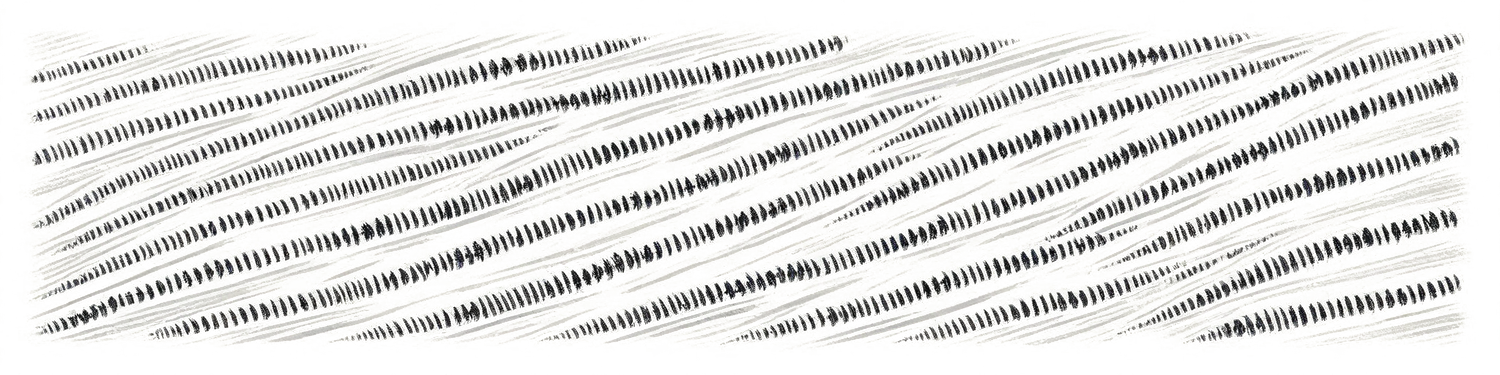
\includegraphics[width=\textwidth]{images/chapterImages/genesis_sketch_00077_.png}
\end{center}

The pattern was complete.

Not finished—it would never truly be finished, could always be refined, could always incorporate more detail. But complete in the sense that all necessary information had been encoded. All critical thresholds marked. All activation timelines established. All probability calculations rendered in stone and space and geometric relationship.

Aurelia stood at the pattern's center and looked at what had been created. Years of work. Thousands of stones. Every piece positioned with mathematical precision. The entire thing functioned as a map, a guide, a set of instructions for creating technological civilization from small mammals across 65 million years.

If it could be read. If anyone survived to read it. If the right minds emerged to interpret geometric relationships as information rather than random scatter.

If. Still always if.

But the work was complete.

879 rotations remaining.

\scenebreak

Around the pattern, the mammals lived their protected lives. The tool-using population had reached stable equilibrium—eighty-seven individuals. Tool use was culturally transmitted. Enhanced cognitive capability was breeding true. Some individuals showed fire-watching behavior. The thresholds were being crossed on schedule.

The tree-dwellers had developed complex social structures. Hierarchies based not just on strength but on problem-solving ability. The clever ones gained status. Gained more breeding opportunities. Intelligence selecting for itself in feedback loop that would amplify across generations.

Other mammal lineages showed different developments. Some had enhanced memory. Others showed better vocal control—the foundation for eventual language. Others showed increased manual dexterity beyond what their ecology strictly required. All selected traits. All guided evolution.

Aurelia had marked each lineage's territory with stones. Not the complex patterns of the main work. Simple markers. Designations. This population carries tool-use genes. This population carries social-complexity genes. This population carries vocal-control genes. When they merged—if they merged—if they survived to merge—the combination of traits would create something greater than any individual lineage.

The markers were arranged geographically to maximize survival probability while maintaining population separation. Distance enough to allow independent evolution. Proximity enough to enable eventual interbreeding once populations grew and ranges expanded.

She had calculated the optimal distribution. Had moved certain mammal populations by capturing and relocating individuals. Transported them in her mouth like prey, carried them miles from their original territories, released them in locations that the mathematics said offered better survival probability and better eventual merger dynamics.

The mammals didn't understand they were being positioned like pieces on a vast board. Didn't know their territories were being optimized. They simply adapted to new locations, bred, continued the cognitive development that had been selected for.

Each population: a different cluster in the pattern. Each cluster marked with specific stones that encoded the genetic modifications that population carried. The entire landscape had become a vast genetic map, readable if one understood the grammar.

\scenebreak

The daughter had completed her own pattern. Smaller than the Watcher's but sound in its mathematics. It focused on a specific section of the larger problem: atmospheric recovery post-impact. Carbon cycle. Oxygen levels. Temperature regulation. Climate return to pre-impact norms over tens of thousands of years.

Her pattern intersected with the Watcher's at key points. Supporting data. Complementary calculations. Two minds working the same problem from different angles, the results reinforcing each other.

The males had contributed their own sections. One focused on ocean recovery—the marine ecosystems would be devastated by impact, but some life would persist in deep waters. That life would reseed the oceans eventually. Understanding that timeline was critical for understanding when coastal populations of evolved mammals could utilize marine resources. When seafaring would become possible. When global connectivity would enable the final technological acceleration.

The other male focused on geological processes. Mineral access. Where certain elements critical for tool-making would be exposed by impact crater formation. Where volcanic activity would resurface useful materials. Where erosion would reveal what needed to be found when the time came.

All of it integrated into the master pattern. All of it connected through mathematical relationship. The scope was staggering. The precision required was impossible. They had achieved it anyway.

Other contributors had added their pieces across the continent. The Builder's pattern focused on the timeline itself—the step-by-step progression from one threshold to the next. Tool use to fire to agriculture to settlements to specialization to writing to mathematics to astronomy to physics to planetary defense. Each step necessary. Each step building on the previous. No shortcuts possible.

The cliff carvings detailed the genetic sequences. Which genes controlled brain size. Which controlled hand dexterity. Which controlled vocal apparatus. Which controlled social bonding. How to select for each. How to combine them. How to create a genome that would support technological civilization.

The patterns didn't contain the genes themselves—that was encoded differently, in the actual genetic material of the living mammals. But the cliff carvings mapped the genome. Explained which sequences mattered. Provided the instruction manual for reading what had been written into living flesh.

\scenebreak

The wrongstar had developed its tail. A bright streak across the sky. Beautiful if one didn't understand what it meant. Terrifying if one did.

Everyone understood.

Across the planet, the work had reached feverish completion. Not panic. Not desperation. Just the recognition that time was finite and the work needed finishing. Every individual capable of contribution contributed. Every mind that could calculate did calculate.

And then, gradually, the work stopped.

Not because it was complete—it could never be truly complete. But because there were no more stones to place. No more cliffs to carve. No more patterns to encode. The information that could be conveyed through physical positioning and geometric relationship had been conveyed. The rest would have to be carried in living flesh. In selected genes. In behavioral instinct encoded so deep that it would persist through 65 million years of evolution.

Aurelia stood in her pattern and waited for the mammals to emerge for evening foraging. They came on schedule. The tool-user led her family group. They foraged efficiently, using tools to access food sources. They shared food with offspring, teaching technique. They demonstrated problem-solving, social cohesion, forward planning.

She watched them with the same intensity she had watched the first tool-user years ago. But now she wasn't observing for new information. She was confirming that the traits had stabilized. That the modifications were complete. That what she had built into them would persist.

The tool-user noticed her watching. Paused in its foraging. They looked at each other across ten body lengths of space. Predator and prey. Creator and creation. Past and future.

The mammal didn't understand what it was. What it carried. What it would become.

Aurelia understood completely.

She made a soft sound. Not aggressive. Not possessive. Just... acknowledgment. The mammal had served its purpose. Had been shaped for a reason. Would carry forward the encoded potential even if it never knew why.

The mammal returned to foraging. Its family followed. They disappeared into the undergrowth.

She didn't follow. Didn't hunt. Just watched them go and ran calculations one more time. Survival probability for that specific lineage: 47\%. Higher than most. The tree-dwellers had 38\%. The social-complexity lineage had 52\%. The vocal-control group had 31\%.

Combined survival probability—at least one lineage persisting through impact winter: 89\%.

Probability that survivors retained the encoded traits: 71\%.

Probability that traits would propagate and amplify over time: 64\%.

Probability that technological civilization would emerge: 23\%.

Probability that civilization would achieve planetary defense before the next major impact: 8\%.

Eight percent.

She had spent years of her life, sacrificed everything that wasn't this work, driven herself and others to the edge of capability. Had calculated across timescales that turned individuals into statistical noise. Had encoded a plan so vast and complex that its mere existence was improbable.

For eight percent.

Eight percent wasn't good. Wasn't remotely sufficient. In any sane framework, eight percent was failure probability masquerading as success chance.

But it was better than zero. Better than extinction guarantee. Better than nothing persisting. Better than the wrongstar hitting an unprotected world and that being the end of possibility forever.

Eight percent was what mathematics and effort and sacrifice could purchase. And so it would have to be enough.

\scenebreak

That evening, the entire family gathered in the territory. The daughter with her mate and hatchlings. The males with their mates. The neighbor pairs who had been working on adjacent patterns. A dozen individuals total. Three generations. All still living to see the project completed.

They didn't gather for ceremony. Their kind didn't do ceremony. But they gathered anyway, drawn by some shared recognition that the work phase had ended. That what came next was different. Was waiting. Was the helpless time when all variables were locked and all calculations were complete and nothing remained but to observe outcome.

They stood in loose formation around the pattern's central section. The master plan. The encoded timeline. The mathematical proof that survival was possible.

The wrongstar rose bright enough to read by. Bright enough to cast shadows. Bright enough that nocturnal creatures were becoming confused, sometimes treating night as day.

No one moved. No one calculated. No one worked. They simply stood together and watched the sky and waited for what would come.

A young one—one of the daughter's hatchlings—broke the silence with a questioning chirp. Too young to understand. Too young to feel the weight of what approached. It was shushed gently by its parent.

Aurelia looked at that young one. Calculated its age. It would be adolescent at impact. Old enough to hunt independently. Young enough that it might survive on less food during the resource-scarce years. Its survival probability was actually slightly higher than the adults'. Small size advantage. Lower caloric requirements. Better hide-and-wait capability.

If it survived, if it bred after the impact, if it passed on any fragment of knowledge...

But that was speculation beyond the scope of current planning. The encoding was complete. The dice were cast. The wrongstar approached on its inevitable trajectory.

836 rotations remaining.

\scenebreak

Over the following weeks, the pattern became... something else. Not abandoned. Not forgotten. But no longer actively worked. It simply existed. A monument to effort. A message to the future. A plan that would either unfold or fail to unfold across time scales beyond imagining.

Life continued around it. The mammals foraged and bred and raised young. The dinosaurs hunted and protected and maintained the selective pressures that shaped the mammal populations. But the feverish intensity was gone. The desperate push toward completion had completed. What remained was maintenance. Waiting. The patient countdown toward event horizon.

Aurelia spent less time at the pattern. More time in simple observation. Watching the mammals. Watching the sky. Watching her family and the neighbors and the whole community of calculation that had emerged around the project.

She hunted more. Needed to rebuild reserves depleted by months of minimal intake. Her body had suffered from the sustained effort. She was thinner than healthy. Her feathers showed damage. She needed recovery time.

But there was recovery time now. 800-some rotations was plenty for physical restoration. The work didn't require her attention anymore. The pattern was stable. The mammals were successfully breeding. The plan was encoded and waiting for its unimaginably distant activation.

She could rest.

She stood sometimes at the marked stone where the other one had been. The grass had grown tall around it. Small flowers bloomed in season. Life continued. Matter cycled. The world persisted in its patterns.

She wondered if he had understood the full scope. If his mathematics had reached far enough forward to comprehend what they were attempting. Or if he had simply contributed what he could calculate and trusted that it connected to something larger.

She would never know. His calculations had terminated. Her calculations continued. And the pattern that incorporated his work would either succeed or fail independent of either of them.

That was the nature of deep time planning. No one would know if it worked. Success would occur so far in the future that it might as well be in a different universe. Causality stretched so thin across 65 million years that the connection between action now and result then became almost metaphysical.

But the mathematics was sound. The encoding was complete. And eight percent was better than zero.

She looked at the wrongstar—now bright enough that it hurt to look directly at it. Developing structure. The tail streaming behind. The signature of terminal approach.

Soon. Very soon now.

The waiting was almost over.


\chapter{The Architects}
\label{ch:10}



\begin{center}
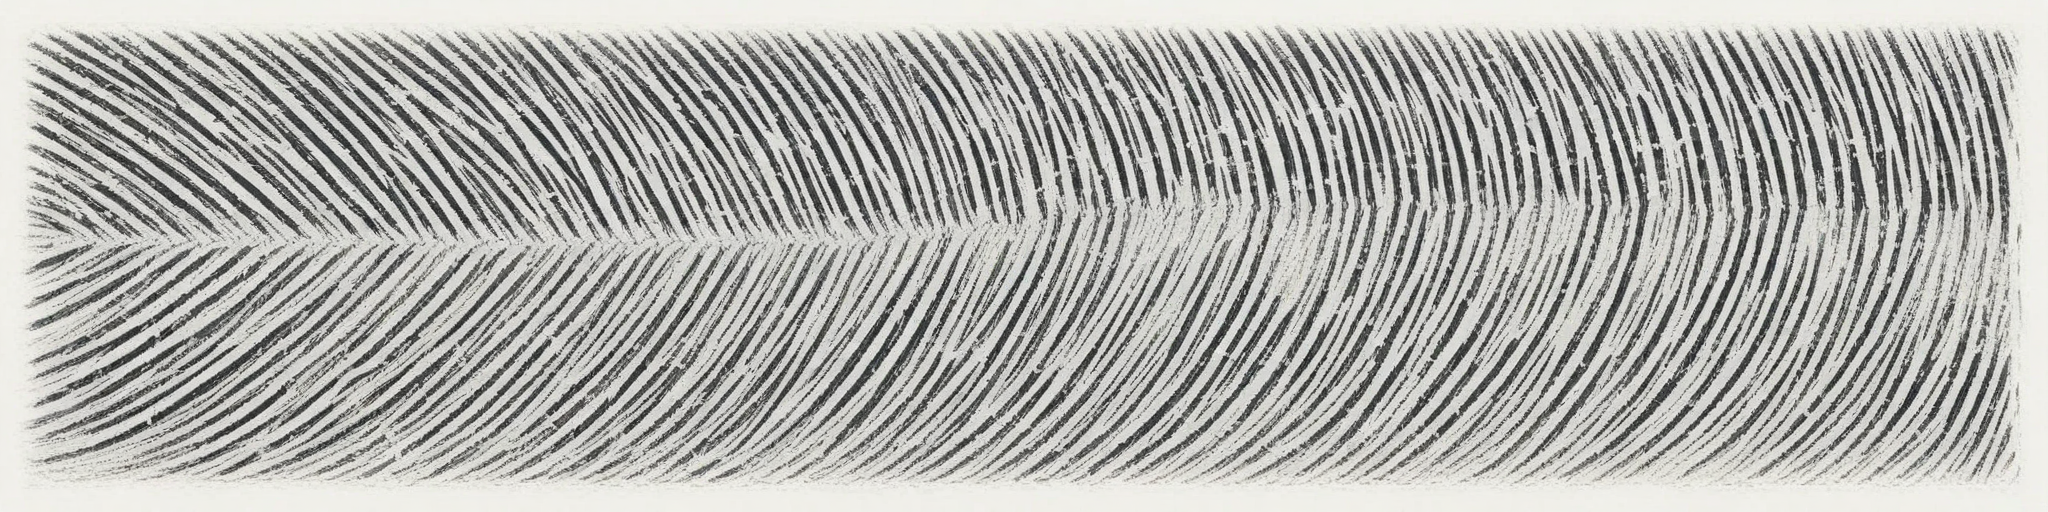
\includegraphics[width=\textwidth]{images/chapterImages/genesis_sketch_00085_.png}
\end{center}

She had been still for forty-two days. The longest calculation yet. Longer even than the master pattern integration. This was different. This was final verification. Final confirmation that everything connected. That every piece of the vast, complex plan fit together into a coherent whole.

Around her, life continued. Her family brought food. The mammals foraged under protection. The wrongstar grew bright enough that it dominated both day and night sky, a burning presence that no one could ignore.

742 rotations remaining.

But she calculated beyond those rotations. Calculated through the impact. Through the extinction. Through the slow, grinding recovery of ecosystems from extremophile survivors. Through the emergence of new dominance hierarchies. Through millions of years of evolution guided by the encoded traits she had selected for.

Tool use at generation 17,000.
Fire control at generation 200,000.
Agriculture at generation 600,000.
Writing at generation 1,500,000.
Mathematics at generation 2,100,000.
Astronomy at generation 2,500,000.
Planetary defense at generation 3,250,000.

Seven thresholds. Seven capabilities. Seven stages from nothing to salvation. She had no concept of the number's significance. Only that the mathematics was complete.

If the activation sequence triggered. If the encoded traits expressed. If evolution followed the calculated path. If civilization emerged. If they developed the capability.

If.

On the forty-second day, the calculation completed. Every variable checked. Every probability confirmed. Every pathway verified. The mathematics was sound. The plan was coherent. The encoding was correct.

Eight percent probability remained eight percent. No refinement changed it. No optimization improved it. Eight percent was the mathematical ceiling given current conditions and available resources and the fundamental constraints of biology and time.

It would have to be sufficient.

She moved.

\scenebreak

The pattern sprawled across the landscape. Thousands of stones positioned with geometric precision. The mathematics made physical. But there was one section left unmarked. One piece that needed closure.

She walked to the marked stone. The place where the other one's matter had dispersed. Grass and small flowers grew around it. The stone itself showed weathering from seasons of exposure. But it remained.

She picked up three small stones from the pattern's edge. Carried them to this location. Arranged them in specific geometry around the marker. The same configuration she had used at the very beginning. The first pattern she had ever created. The foundation from which everything else had grown.

Three stones. Simple. Primary. Complete.

The configuration meant something. Encoded specific information. But it also meant nothing except to her. Personal notation. Acknowledgment. Recognition that his contribution mattered to the calculation even if his matter no longer existed in assembled form.

The stones were placed. The marker was complete. She stepped back and looked at what she had created.

Then she returned to the pattern's center and began the final verification walk.

\scenebreak

She moved through the entire pattern. Every section. Every subsection. Every cluster of stones that encoded specific information. Her movement was methodical, systematic. She examined each placement, confirmed each relationship, verified each calculation rendered in physical form.

The daughter's atmospheric recovery section: mathematically sound.

The male's ocean recovery section: correct.

The other male's geological processes section: verified.

The neighbor's contributions to genetic mapping: accurate.

The Builder's timeline: complete.

The Carver's genetic sequences: preserved in stone.

Every piece checked. Every connection confirmed. The entire vast edifice of planning and calculation and desperate hope holding together as coherent whole.

The verification walk took three days. When she finished, she returned to the center and stood looking at the mammal territories visible from this position. The tool-users to the east. The tree-dwellers to the west. The social-complexity group to the north. All visible from this central point. All marked. All prepared.

The wrongstar filled a quarter of the sky now. Its tail streamed behind it like a banner. The heat from it could be felt even during the day. The end was approaching not as abstract calculation but as visible, tangible reality.

She watched the tool-user territory until the mammals emerged for evening foraging.

\scenebreak

The family group appeared on schedule. Nine individuals. The original tool-user—elderly now by mammal standards, moving more slowly but still alive—led the group. Younger adults followed. Adolescents bounded ahead with excess energy. Infants clung to parents' backs.

The original tool-user paused at the entrance to its burrow. Bent down. Picked up a stick.

It was a specific stick. The one it had been using for seventeen days now. Shaped through use into optimal configuration. One end worn smooth from handling. The other end sharp from repeated insertion into insect colonies.

The mammal examined the stick. Tested its weight. Checked the sharpness of the working end. Then it set the stick down carefully at the burrow entrance. Deliberately. Precisely. In a specific position where it could be easily found tomorrow.

It would use that stick again tomorrow. And the day after. Would use it until it broke or wore out, then create another like it. Had already taught the technique to offspring, who practiced with their own sticks. Had demonstrated the optimal shape, the best working techniques, the maintenance procedures.

Aurelia had waited seventeen generations for this mutation.

\scenebreak

The small creature extracted grubs from the rotted log with the stick, ate them one by one, then set the stick aside carefully, deliberately, for reuse. Tool creation. Tool maintenance. Tool culture. Everything she had selected for, now expressing reliably across a population.

The creature would not understand for millions of years.

None of them would.

But they would discover fire when their population density reached the threshold she had calculated. They would develop agriculture when the climate stabilized 10,000 rotations after impact. They would invent writing when their vocal structures evolved the three specific markers she had selected for in generation forty-three of the breeding program.

They would look at the stars, and something buried deep in structures she had carefully, painstakingly encoded, would whisper: *calculate*.

They would call it curiosity.

They would call it genius.

They would call it inspiration.

They would wake at dawn with ideas they couldn't explain. Would feel driven to create things they didn't understand the purpose of. Would sacrifice comfort, stability, relationships—for the work. And they would never know whether the drive came from within or was whispered through time by careful hands.

She had called it activation.

They would be so proud of each discovery. So certain of their own brilliance. They would build towers of achievement and call themselves the authors. They would trace their history and see nothing but their own clever progression from simple to complex.

They would never know that every threshold had been programmed. That every breakthrough was scheduled activation. That their entire civilization was executing code written 65 million years ago by minds that could hold entire evolutionary timelines in conscious calculation.

She had done this for him.

For their hatchlings who died before understanding. For the other one who helped even when he couldn't fully comprehend the scope. For every individual who contributed what they could calculate and trusted that it mattered to something larger.

The small mammals would never know the cost. Would never know that every human—she had no word for what they would call themselves, but they would be human in form and function—every human who felt something for their children, who worked to build something beyond themselves, who sacrificed for a future they wouldn't see—was echoing her.

That feeling wasn't in the code.

That feeling was why there was a code at all.

The mathematics could encode capability. Could schedule activations. Could guide evolution through millions of years toward specific endpoint. But the impulse to create the code—the reason to spend years in desperate effort, to sacrifice everything, to calculate across time scales that made individual existence meaningless—that impulse couldn't be programmed.

That impulse was the only thing that was real.

And it would propagate forward not through genetic encoding but through the simple fact of consciousness recognizing the value of its own continuance. Through minds that understood mortality calculating ways to transcend it. Through life that knew it would end working to ensure something else would begin.

The mammals would feel it too. Millions of years from now. They would look at their own extinction probability and calculate ways to reduce it. Would build their own desperate plans. Would sacrifice their own present for an uncertain future. Would encode their own gifts for civilizations they would never meet.

And they would think they chose it. Would believe the impulse was theirs. Would call it noble or necessary or just what intelligent beings do.

They would be right and wrong. The impulse would be theirs. But the capability would be hers. The activation would be scheduled. The timeline would unfold as calculated.

Or it wouldn't.

The mammal finished with the stick. Cached it carefully. Led its family to new foraging territory. Disappeared into the undergrowth.

Aurelia stood watching the empty space where they had been. Ran the calculation one final time. From this moment forward across 65 million years to planetary defense capability.

Eight percent.

She returned to stillness. The verification was complete.

\scenebreak

Somewhere, 65 million years in a direction she could not imagine, in a time that made the calculation of it feel like abstraction rather than eventual reality, a human woman stared at a computer screen.

The genetic sequence made no sense. Too regular. Too purposeful. Repeating elements that shouldn't repeat. Mathematical relationships encoded in DNA that should be random noise.

She highlighted the first cluster. Ran correlation analysis against neural development markers.

Tool use.

The structures in the human brain that enabled hands to manipulate objects with precision. That linked visual processing to motor control. That allowed abstract representation of physical relationship. All encoded in a specific genetic sequence. All activating at a specific point in evolutionary timeline.

Her hand trembled as she highlighted the second cluster.

Fire control. The reduced fear response to flame. The enhanced pattern recognition for combustion conditions. The cognitive structures that enabled risk assessment and controlled use of dangerous elements.

Third cluster. Agricultural timing. Seasonal awareness. Plant domestication capability. Long-term resource planning.

Fourth. Fifth. Tenth. Twentieth.

Every major human capability. Every threshold that separated homo sapiens from our ancestral primates. Every innovation that built civilization.

All encoded. All scheduled. All activated according to timeline that existed before humanity existed.

She sat back from the screen. The laboratory was silent. The implications were...

She couldn't process the implications. Not yet. First she needed to confirm. To verify. To check every calculation and make certain she wasn't seeing pattern where only noise existed.

But the mathematics was sound. The correlation was too strong to dismiss. The activation timeline matched archaeological record with precision that couldn't be coincidental.

Humanity was not the author of its own progress.

Humanity was executing a program.

\scenebreak

Aurelia returned to stillness. The calculation was complete. The verification was done. The message was encoded in stone and flesh and the patient mathematics of deep time.

742 rotations remaining.

She would spend them in preparation. In ensuring the mammals had maximum survival probability. In making final adjustments to the pattern. In waiting for the inevitable.

But the work was finished. The plan was complete. The activation sequence was set.

In 65 million years, a species that didn't yet exist would read the pattern. Would understand what they were. Would know that every achievement they claimed was gift from extinct intelligence that loved its world enough to ensure something survived.

And they would build the defense grid. Would detect the next asteroid. Would redirect it. Would protect the planet from the catastrophe that was coming—not for them, but for something that would come after them. Some next iteration of consciousness that didn't yet exist but would, if the pattern held, if the mathematics was sound, if the activation sequence continued forward into time scales that made 65 million years look brief.

The cycle would continue. The protection would propagate. The code would execute across geological epochs. And consciousness—that strange emergent property of matter organized in specific configuration—would persist.

Not any specific consciousness. Not her or the mammals or the eventual humans or whatever came after. Just consciousness itself. The universe's way of experiencing itself. Of calculating its own continuation. Of choosing to persist rather than to end.

If that's what choice meant.

If choice existed at all.

If it mattered whether it did.

Aurelia stood still as stone itself. The wrongstar burned above. The mammals lived their protected lives. The family maintained the territories. The pattern existed complete and verified and ready for eventual reading.

The mathematics was complete.

And somewhere in a direction that time flowed forward toward, a human woman sat staring at a screen and feeling the ground drop away beneath her understanding, feeling everything she thought she knew about human achievement invert and collapse into a new configuration that was somehow both devastating and beautiful.

We were never alone. We were never the first. We were never the authors.

We were the inheritors. The activation. The execution of a plan so vast and patient that it made human timescales look like heartbeats.

And the dinosaurs who wrote it were so incomprehensibly intelligent that they could calculate 65 million years forward and encode the result in genetics and stone and mathematical relationships that persisted through extinction.

We called ourselves sapiens. Wise.

They called us activation sequence.

And they had been right.


\chapter{The Completion}
\label{ch:11}


The work had shifted from creation to preservation. Nothing new could be added. The mathematics was complete. The encoding was finished. What remained was optimization—ensuring maximum survival probability for what already existed.

400 rotations remaining.

The wrongstar no longer looked like a star. It looked like what it was: a massive object approaching collision. During the day, it was a bright disk with streaming tail. At night, it dominated the entire sky, washing out all other celestial objects. The heat from it was measurable. Subtle, but present. The planet was already beginning to warm from the radiation.

The Watcher moved through the mammal territories with systematic precision. Each protected population needed final positioning. Not where they lived now—where they needed to be when the impact came.

\scenebreak

The tool-using population had grown to 143 individuals. Too large. Too concentrated. A single fire or disease could eliminate the entire lineage. She needed to split them.

She began the separation carefully. Captured specific individuals—always at night, always swiftly, minimizing stress. Transported them in her mouth like prey, their small bodies trembling against her tongue. Carried them for miles. Released them in locations that her calculations said offered optimal survival probability.

Mountain valleys with cave systems for shelter. Regions with diverse food sources. Areas with natural barriers that would protect against the worst of the impact shockwave. Each location chosen through mathematical analysis of wind patterns, temperature disruption, resource availability post-impact.

She split the tool-using population into seven groups. Each group carried the full genetic package. Each group positioned in geographically isolated territory. If one group died, six others remained. If three groups died, four remained. The redundancy was essential.

The mammals didn't understand why they were being relocated. Didn't know that the creature who should eat them was instead saving them. They adapted because adaptation was what they did. Established new territories. Began foraging in new ranges. Within days, they functioned as if they had always been there.

The tree-dwellers she split into five groups. The social-complexity mammals into six groups. The vocal-control lineage into four groups. Each splitting carefully calculated to maximize survival probability while maintaining genetic diversity.

The work took thirty rotations. By the end, protected mammals existed in forty-three separate locations across the continent. Each location chosen for specific survival advantages. Each population carrying specific encoded traits. Each group isolated enough that disease or disaster couldn't eliminate multiple lineages simultaneously.

When all groups were positioned, she stood at a high ridge and looked across the landscape. From here, she couldn't see any of the protected territories. But she knew where each one was. Held the map complete in her mind. Forty-three points of light in the darkness that was coming.

The probability calculations shifted with the improved distribution. Overall survival: 89\% to 94\%. At least one lineage persisting: 97\%. Multiple lineages surviving: 82\%.

The numbers were better. Still not certain. But better.

\scenebreak

The pattern remained where it was. Couldn't be moved. Couldn't be protected. The impact would destroy it—not immediately, but the climate disruption would erode the careful stone placements, scatter the configuration, reduce it to meaningless rubble within decades.

That was acceptable. Expected. The pattern wasn't meant to survive. It was meant to exist long enough that the information could be verified before impact. That verification was complete. What mattered now was the encoding in living flesh. The genetics. The code written into DNA that would persist through extinction and emerge on the other side.

Still, she visited the pattern each evening. Walked through its sections. Not working anymore. Just... present. Recognition of what had been achieved. Acknowledgment of the effort that had gone into creating this temporary physical instantiation of deep-time mathematics.

Her family had dispersed to their own territories. The daughter maintained protection of one mammal group. The males protected others. They had learned the work. Could continue it without her guidance. The network of protection would hold through the final rotations. Would hold even after impact, if any of them survived to maintain it.

The young pairs who had worked on adjacent patterns had moved to their own chosen territories. Some near protected mammal populations. Others near the gathering points where final vigil would be kept. All of them understanding their purpose. All of them accepting what was coming.

The species had achieved something remarkable in these final years. Not technology—they had never needed technology. Not civilization—they had never organized into cities or formal structures. But collective understanding. Distributed intelligence working toward common purpose. Mathematics shared across thousands of minds, each contributing what they could calculate.

If intelligent life was measured by tool use and language and built environment, her kind would seem primitive. Animal-like. Operating on instinct.

But if intelligence was measured by depth of calculation, by capacity to process complexity, by ability to plan across timescales that made individual existence irrelevant—then her kind was more intelligent than anything that would come after for 65 million years.

The mammals would eventually surpass them. Would develop capabilities the dinosaurs never needed. Would build machines to extend their cognitive capacity. Would create tools to overcome their biological limitations.

But they would do it because she had encoded the capability. Would follow the path she had calculated. Would achieve technological civilization not through their own brilliance but through activation of sequences she had designed.

They would never know. Would believe themselves the authors. And that was acceptable. Expected. The activation sequence worked better if the activated didn't recognize they were executing code.

Self-aware tools were less efficient than tools that believed themselves autonomous.

\scenebreak

The wrongstar grew brighter. The days grew warmer. Strange weather patterns emerged—winds that shouldn't exist, temperature inversions, storms forming without apparent cause. The planet's systems were already beginning to destabilize from the approaching mass, from the gravitational disruption, from the radiation heating the upper atmosphere.

Small animals behaved strangely. Migration patterns disrupted. Breeding cycles confused. Some creatures seemed to sense what was coming and fled toward regions that offered no better survival probability than where they'd been. Panic behavior. Instinct misfiring in the face of threat too large to comprehend.

The dinosaurs didn't flee. Didn't panic. They continued their preparations with calm efficiency. Moved to the territories they had chosen. Gathered with family groups. Maintained protection of the mammal populations through the chaos. Did what needed doing until there was nothing left to do.

The Watcher spent one final day verifying mammal positions. Visited each of the forty-three protected territories. Confirmed that populations were established, food sources were adequate, shelter was available. Made minor adjustments where necessary—drove away a predator here, cleared a den entrance there. Small optimizations that increased survival probability by fractions of a percent.

Fractions mattered when survival was already marginal.

When the verification was complete, when every population was positioned optimally, when no further improvements were possible, she returned to her original territory. To the clearing where the pattern existed. To the marked stone where the other one had dispersed years ago.

The three small stones she had placed around the marker remained undisturbed. The geometry was still precise. The grass had grown tall around them, but the stones themselves were exactly as she had positioned them.

She stood there as the sun set and the wrongstar rose—now so bright it cast shadows sharper than moonlight. In ten rotations, it would be too bright to look at directly. In fifty rotations, the heat from it would begin killing vegetation. In 400 rotations...

In 400 rotations, the equation would balance.

She had done everything mathematics could calculate. Had positioned every variable optimally. Had encoded every necessary instruction. Had built redundancy into every system. Had maximized probability within the constraints of biology and physics and time.

Eight percent chance of full success. Ninety-seven percent chance of something surviving. Numbers that would have to be sufficient because they were the maximum achievable given available resources and fundamental limitations.

The work was complete.

What remained was waiting. And the patient countdown toward inevitability.

\scenebreak

She returned to her hollow one final time. The space was empty now—her daughter had moved to her own territory. But the hollow retained the shape of bodies that had pressed into it over years. The worn smoothness of repeated use. The small modifications made for comfort. Evidence of occupation. Of life lived here. Of function fulfilled.

She settled into the space. It fit her form exactly. Familiar. Optimal. Home in the simple sense that this was where her body had rested, where she had processed calculations during sleep, where she had survived through the years of preparation.

Tomorrow she would leave it. Would move toward the gathering point. Would stand with others and watch the final approach. Would witness the impact if she survived the initial shockwave. Would die knowing that the mathematics was sound even if the outcome was uncertain.

But tonight, she rested in familiar space. Let her body recover what it could recover. Processed the final calculations one more time not because they needed processing but because the habit was ingrained. Because calculation was what she did. What she had always done. What she would do until consciousness terminated.

The wrongstar burned bright enough to illuminate the hollow's interior. Bright enough that shadows moved as it climbed across the sky. Bright enough that darkness had become a memory rather than a nightly reality.

370 rotations remaining.

The countdown continued its patient advance toward zero.

And in forty-three locations across the continent, small mammals slept in their burrows, carrying genetic code they didn't know existed. Carrying capability they wouldn't use for thousands of generations. Carrying the future of consciousness on a planet that was about to be devastated.

They were so small. So fragile. So utterly vulnerable to what was coming.

But they had one advantage: they could hide. Could burrow deep. Could survive on minimal resources. Could persist through conditions that would kill larger organisms.

And they carried the code.

That would have to be enough.

The Watcher closed her eyes. Sleep came slowly, interrupted by the unnatural brightness, by the warmth that shouldn't exist at night, by the approaching termination of everything she had worked for.

But eventually, sleep came.

And the calculations continued even in sleep, refining themselves, optimizing until the very last moment of consciousness, because that was what intelligence did. That was what mattered.

Calculate. Optimize. Persist.

Until persistence was no longer possible.

Then: disperse. Return to constituent elements. Let the plan unfold without you because you encoded it well enough that your presence was no longer necessary.

The mathematics was complete.

The work was done.

What remained was aftermath.

And hope, if that's what one called probability calculations rendered in living flesh and given 65 million years to resolve.


\chapter{The Witness}
\label{ch:12}


The young one had been watching for seventeen days now.

She was not of the Watcher's family. Not even from particularly close territory. But she had traveled here deliberately, drawn by something she couldn't have named but felt with absolute certainty. The work happening in this clearing mattered. Was important in ways that exceeded individual survival or territory or the normal calculations of existence.

She was young—barely into adolescence, her feathers still showing juvenile patterning, her movements not yet settled into adult efficiency. But her eyes were sharp. Her attention unwavering. She watched everything the Watcher did with focus that suggested intelligence beyond her years.

Or perhaps simply intelligence at the threshold. The moment when capability exceeded instinct. When observation became more than simple mimicry. When understanding began, even if full comprehension remained impossible.

287 rotations remaining.

The wrongstar was a constant presence now. Day and night merged into a single bright existence. The heat was notable—not deadly yet, but moving in that direction. Plants were beginning to show stress. Some animals had already died from the disruption to their food sources, to their environmental tolerances, to the simple fact that the world was changing too fast for adaptation.

But the young one endured. Watched. Learned what she could learn.

\scenebreak

The Watcher was aware of the observer. Had been aware from the first day. But she didn't drive the young one away. Didn't signal threat or territorial defense. Just continued her work while being watched.

The pattern was unchanging now—no new stones added, just verification walks. But the verification had purpose. Each walk confirmed that relationships still held, that the encoding remained intact, that erosion or animal activity or the increasingly violent weather hadn't disrupted critical elements.

The young one followed these verification walks at a respectful distance. Stopped when the Watcher stopped. Moved when she moved. Tried to see what was being seen, understand what was being confirmed.

On the eighth day of observation, the young one had approached the pattern's edge. Carefully. Uncertainly. Watching for signs of rejection or aggression. Finding none.

She examined a small cluster of stones—a simple subsection dealing with temperature recovery post-impact. The mathematics was relatively basic compared to other sections. Within her capacity to begin understanding, if not to fully calculate.

She tilted her head. Studied the arrangement. Saw relationship between stones that wasn't random. Saw pattern that encoded meaning.

Then she picked up a small pebble and placed it.

The placement was wrong. Completely wrong. Disrupted the local mathematical relationship. Created dissonance in the pattern's grammar.

The Watcher had been twenty body lengths away, conducting verification of a different section. She stopped immediately. Turned. Looked at the young one and her terrible stone placement.

The young one froze. Recognized her error. Waited for correction or punishment or rejection.

The Watcher approached. Examined the misplaced pebble. Removed it. Set it aside. Then selected a different small stone and placed it in the location the young one had attempted. The correct position. The proper relationship. The mathematics restored.

She stepped back. Looked at the young one. Waited.

The young one approached the corrected position. Examined it carefully. Compared it to where she had placed her stone. Saw the difference. The shift in angle. The change in distance. The way this position harmonized with surrounding stones while hers had created discord.

Learning. Not through instruction. Through observation and correction. Through seeing right answer after attempting wrong answer.

She picked up another small stone. Looked at the pattern. Calculated what she could calculate with her limited depth. Placed the stone.

Wrong again. But less wrong. Closer to correct relationship.

The Watcher adjusted it. Showed the proper position.

The young one studied the correction. Chirped softly—a sound of frustration maybe, or recognition of difficulty, or simple vocalization tied to cognitive effort.

She tried again. Another stone. Another placement. Another approximation of proper relationship.

The Watcher adjusted it again.

They continued this way for hours. The young one attempting. The Watcher correcting. No verbal instruction. No demonstration beyond the correction itself. Just the patient repetition of attempt, correction, observation, refined attempt.

By evening, the young one's placements required smaller corrections. She was grasping the local grammar even if the deeper mathematics remained beyond her. She could see relationship. Could recognize harmony versus discord. Could approximate correct positioning.

It was crude. Limited. A child's understanding of concepts that required adult cognition to truly grasp. But it was understanding. The beginning of comprehension. The threshold moment when observation became knowledge.

\scenebreak

Over the following days, the young one worked on her own small pattern at the clearing's edge. Separate from the Watcher's work. Her own contribution in her own limited scope.

The pattern she created was simple. Elementary mathematics. Temperature relationships. Basic survival thresholds. The kind of calculations any adult of their species could manage. But she worked with intensity that suggested she understood this mattered. That her contribution, however small, connected to something larger.

The Watcher observed this work without interfering. Let the young one calculate at her own level. Make her own decisions. Create her own expression of the shared purpose that had drawn her here.

Sometimes the young one would stop her work and watch the Watcher instead. Study the verification walks. Observe the way the Watcher examined each section, confirming relationships, maintaining the integrity of the encoding. Learning not just the mathematics but the method. The approach. The consciousness required to hold complex pattern complete while examining individual elements.

She couldn't achieve that consciousness yet. Her mind wasn't developed enough. But she was learning what adult consciousness looked like. What it could achieve. What was possible if she survived to full cognitive maturity.

If. That word had become omnipresent. If she survived. If anyone survived. If the plan worked. If the encoding persisted. If consciousness continued on this planet after the impact restructured everything.

If.

\scenebreak

On the twenty-first day of observation, the young one completed her small pattern. She stood back and examined it with what might have been pride or might have been simple satisfaction at task completion. The mathematics was sound within its limited scope. The relationships were correct. The encoding would persist until erosion or impact destroyed it, just like everything else.

She looked at the Watcher. Made a soft sound—not quite a question, not quite a statement. Just vocalization that meant something like: is this acceptable?

The Watcher approached the young one's pattern. Examined it section by section. Found it mathematically correct. Limited but correct. A valid contribution to the collective encoding even if its scope was small.

She made a sound back. Acknowledgment. The young one had done well. Had contributed what she was capable of contributing. Had participated in the work at her level of capability.

That was all anyone could do. The Watcher had contributed calculations that reached 65 million years forward. The young one had contributed calculations that reached perhaps a few thousand years forward. The scope differed vastly. But both were valid. Both mattered to the whole.

The young one settled near the Watcher's hollow that evening. Not inside—that would have been presumptuous. But nearby. Close enough to be present. Close enough to continue learning by proximity.

The Watcher allowed it. The young one's presence changed nothing about the work or the timeline or the outcome. But it confirmed something important: the understanding had spread. The knowledge was distributed. Even young minds that couldn't calculate the full depth grasped that something significant was happening. That participation mattered. That contribution at any level exceeded non-contribution.

\scenebreak

More young ones arrived over the following days. Two males. Another female. All adolescent. All drawn by the same inexplicable certainty that this place, this work, this final countdown mattered more than territory or hunting or the normal concerns of existence.

They watched. They learned what they could learn. They created their own small patterns at the clearing's periphery. Their own limited contributions to the collective encoding.

The Watcher didn't instruct them. Didn't coordinate their efforts. Just continued her verification work while they observed and contributed what they could contribute. The teaching happened through observation. Through correction when they attempted to add to her pattern. Through the simple presence of deep intelligence demonstrating what intelligence could achieve.

By 200 rotations remaining, seven young ones had established presence at the clearing. Seven small patterns surrounded the Watcher's massive central configuration. Seven limited but valid contributions to the collective work.

They hunted together. Shared food. Maintained each other's patterns when one was absent. Formed loose social structure based not on family relationship or territorial proximity but on shared purpose. On common understanding that they were witnessing something significant. Participating in something that exceeded individual existence.

None of them would survive the impact. They were young—fast and clever but lacking the experience and deep survival knowledge of older adults. Their probability calculations showed margins too thin to offer real hope. Maybe one would survive if everything went optimally. Probably none would.

But they participated anyway. Calculated what they could. Encoded what they understood. Added their voices to the chorus of mathematics that had emerged across the species during these final years.

And in their presence, in their efforts, in their limited but earnest contributions, the Watcher saw the answer to a question she hadn't fully articulated:

Would the understanding persist? Would future consciousness recognize what had been achieved here? Would anyone remember, even if the patterns themselves were destroyed?

The young ones couldn't answer that. Wouldn't survive to carry memory forward. But they proved that the recognition could exist. That even limited minds could grasp that something larger was happening. That intelligence, however brief its existence, could participate in projects that exceeded its lifespan.

The mammals would do the same eventually. Would recognize, however dimly, that they were part of something vast. Would feel the activation sequences triggering without understanding what they felt. Would build and discover and achieve while believing themselves autonomous, just as these young ones built their small patterns while not fully grasping the larger structure they contributed to.

Perhaps that was sufficient. Perhaps consciousness didn't need to understand its own encoding to fulfill its purpose. Perhaps the execution mattered more than the comprehension.

\scenebreak

As 150 rotations approached, the young ones began drifting away. Not abandoning the work. Just recognizing that their time here was complete. That they had learned what they could learn. That their contributions were finished. That what remained was the final countdown, and that was not theirs to witness.

They needed to return to their own territories. Find their own places for the end. Be with whatever family or companions they had formed. Face the impact in their own chosen locations.

One by one, they departed. Each taking a final look at the pattern—both the Watcher's vast configuration and their own small contributions. Each carrying forward whatever understanding they had achieved. Each having participated in something that exceeded them.

The first young one—the female who had watched longest, learned deepest—was last to leave. She stood at the edge of her completed pattern and looked at the Watcher across the clearing.

They regarded each other for a long moment. Young mind and old mind. Limited calculation and vast comprehension. Student and teacher, though neither had sought those roles.

Then the young one turned and left. Moved into the forest with the efficient grace of her kind. Disappeared into the growing brightness as the wrongstar made even the forest interior visible at all hours.

The Watcher watched her go. Calculated her survival probability one more time: 12\%. Better than most young ones. Still not good.

But she had learned. Had contributed. Had grasped something of the purpose. Had participated in the collective work of encoding consciousness's continuation across deep time.

And if that was all existence offered—brief participation in something larger before inevitable termination—then she had achieved what existence permitted.

The clearing was empty now except for the Watcher. The patterns remained. The wrongstar burned. The countdown continued.

138 rotations remaining.

Time to begin the final journey. Time to gather with others at the places chosen for witness. Time to watch the mathematics resolve into physical reality.

Time to learn whether eight percent was sufficient.

Or whether it wasn't.

Either way, the calculation was complete. The encoding was finished. What remained was observation of outcome.

And then dispersion into the constituent elements from which new patterns would eventually emerge.

If the mathematics held.

If.


\chapter{The Silence}
\label{ch:13}


The wrongstar filled a third of the sky now. Not a point. Not a disk. A presence. Massive enough that its shape was visible—irregular, tumbling slowly, the surface showing variations in brightness where different materials reflected differently. The tail streamed behind it like fire, stretching halfway across the visible sky.

45 rotations remaining.

The heat was constant. Day and night had lost meaning. There was only bright and brighter. Hot and hotter. The temperature had risen enough that many plants had stopped functioning. Forests showed signs of stress—leaves curling, trees dropping foliage early, whole sections of vegetation beginning to die from the sustained thermal assault.

Animals fled in random directions. Migrations that made no evolutionary sense. Instinct firing desperately in the face of threat too large to comprehend. Most would die from the disruption alone, before the impact even occurred. The ecosystem was already collapsing under the strain of approaching catastrophe.

But the dinosaurs remained calm. They had calculated this. Expected this. Knew that the pre-impact effects would be devastating. Knew that it didn't matter because the impact itself would be so much worse that these preliminary deaths were rounding errors in the final total.

They moved toward their chosen places. Gathered with intention. Prepared for ending.

\scenebreak

The Watcher left her territory for the final time. The pattern would remain where it was. Already showing erosion from the violent weather. Stones displaced by wind. Sections disrupted. The encoding degrading as she had always known it would.

It had served its purpose. Had existed long enough for verification. For contribution to collective understanding. For demonstrating that the mathematics was complete. What happened to it now was irrelevant.

She traveled toward the northern plateau—a high, exposed location far from the predicted impact site but with clear lines of sight in all directions. A place where watching would be unobstructed. Where the final calculations could be confirmed through direct observation. Where consciousness could witness its own ending with full awareness of what was ending and why.

Others moved along parallel paths. She could sense them without seeing them. The feeling of presence that came from shared direction, shared purpose. They were all converging on gathering points. Not randomly. Not instinctively. Through calculation that had identified optimal witness locations given impact trajectory and shockwave propagation patterns.

The journey took four rotations. She didn't hurry. Didn't conserve energy. There was no need for conservation anymore. No future that required physical reserves. Just the present moment extending forward for 45 more rotations until it terminated.

When she arrived at the northern plateau, dozens were already there. More appeared as she watched—individuals and small family groups emerging from different directions, all converging on this calculated point.

The massive long-necks stood at the plateau's edge, their huge bodies somehow appearing fragile against the scale of sky-filling wrongstar. The swift runners clustered together, their speed advantage meaningless now. The armored ones had shed their defensive postures—no threat remained that armor could stop.

And everywhere, the small ones. The thinkers. The calculators. Hundreds of them. Standing in loose formation that somehow organized itself without coordination. Each individual finding a position that felt correct. That fit the mathematics of optimal witness configuration.

The Watcher found her position. It was waiting for her—not marked, not designated, just recognized as correct when she arrived at it. She settled into stance and looked at the sky.

Around the plateau, other gathering points were similarly occupied. She couldn't see them but knew they existed. The calculations had identified seventeen optimal witness locations given global distribution and viewing angle requirements. All seventeen would be occupied. All seventeen would observe the same event from different perspectives. Final data collection. Last confirmation that the trajectory calculations were correct.

Not that it mattered if they were correct. There was no time left for adjustments. No possibility of evasion. The wrongstar would arrive where calculations said it would arrive. Would impact with the energy calculations predicted. Would reshape the planet according to mathematical certainty.

But they would watch anyway. Would confirm the calculations through observation. Would witness the accuracy of their predictions even as those predictions manifested as extinction.

Because that's what consciousness did. Observed. Calculated. Understood until understanding was no longer possible.

\scenebreak

The Builder arrived at the plateau on the third day of gathering. The Watcher recognized him immediately—he had changed since she'd last seen him years ago, scarred and aged by the intensity of his work. But his posture was unmistakable. His movement patterns. The particular quality of stillness he achieved.

He found his position and settled. They were perhaps fifty body lengths apart. Close enough to acknowledge each other's presence. Far enough to maintain individual observational integrity.

They had never directly interacted. Had never shared calculations through anything but the patterns they created independently. But they had worked the same problem. Had arrived at the same solutions. Had encoded their understanding in complementary ways that together formed complete picture.

Acknowledgment passed between them without signal. Just recognition. Just presence. Just the understanding that they had both contributed what they could contribute and now would both witness what that contribution led to.

The Carver never arrived—she had died seasons ago, her work complete. But two of her protégés were present. Young ones who had learned her cliff-carving techniques. Who had added their own sections to the genetic encoding she had begun. Her understanding persisted through them. Her contribution continued through their extensions of her work.

That was sufficient. That was the only form of persistence available to consciousness. Through the work that outlived the worker. Through the knowledge that propagated beyond the knower. Through the calculations that remained valid independent of who had calculated them.

\scenebreak

More arrived. The gathering swelled to hundreds, then thousands. Not every dinosaur on the continent—most had chosen locations closer to their home territories, places significant to their individual experience. But enough gathered here to create the feeling of collective witness. Of shared observation. Of consciousness recognizing itself in multitude before that multitude dispersed forever.

They stood in silence. Not the silence of absence but the silence of complete understanding. No communication was necessary. All calculations were complete. All knowledge was shared. What remained was waiting.

And watching.

The wrongstar grew daily. Hourly. The tumble of its rotation became visible—brighter patches rotating across its surface, darker regions disappearing and reemerging. The detail increased as distance decreased. Soon individual surface features would be distinguishable. Later, the shape would dominate everything. Fill the entire sky from horizon to horizon.

Then: arrival.

The timeline was absolute. 45 rotations at the gathering's start. Now 42. Now 38. Now 33. The countdown continued with mathematical precision. Each rotation confirmed the calculations. Each observation matched prediction. The trajectory was perfect. The impact was inevitable. The extinction was certain.

And they watched it approach with calm acceptance that might have looked like peace if peace was the right word for understanding your own termination.

\scenebreak

On the twentieth rotation before impact, the Pair arrived.

She hadn't seen them since before the work began. Since before the wrongstar had appeared. They had been separate for years—working in distant territories on their own patterns, their own contributions.

Now they were together again.

They entered the gathering side by side. Moving in perfect synchronization. Steps matched. Breathing aligned. They found a position near the plateau's center and settled together. Not just near each other. Pressed together. Flanks touching. Tails intertwined. Physical contact that was constant and complete.

The Watcher observed this with the detached interest of someone watching mathematics resolve into behavior. They had maintained connection across vast distance through unknown means. Had worked separately while somehow remaining unified. Had calculated independently while arriving at identical conclusions. Now they reunited for the final witness.

They were older now. One of them showed significant age—feathers thinned, movements slow, breathing labored. The other was healthier but not much. They had both pushed themselves to the limit of biological capability during the work years.

They would not survive the impact. Their survival probability calculations were essentially zero. They were too old, too worn, too depleted. The impact winter would kill them within days even if the initial shockwave didn't.

They knew this. The calculations were simple enough that even less sophisticated minds could run them. They knew they were dying soon regardless of what they did.

And they had chosen to die together. Pressed against each other. Unified until the end.

The Watcher watched them and understood something that mathematics couldn't quite capture: the work was necessary, but it wasn't sufficient. The encoding mattered, but it wasn't everything. Connection existed that couldn't be quantified. That persisted despite separation. That manifested as physical proximity in final moments not because proximity increased survival probability but because it provided something else. Something the calculations couldn't incorporate but that consciousness required anyway.

She thought of the other one. The one who had helped with her pattern. Who had brought food. Who had stood with tail almost touching. Who had dispersed years ago into constituent elements and couldn't be here for final witness.

She had marked his location. Had continued his pattern section. Had maintained his contribution. But he wasn't present. Couldn't be present. Matter didn't reassemble once dispersed. Consciousness didn't persist beyond biological function.

The Pair demonstrated an alternative: be together until the end. Maintain physical connection. Let the termination happen while unified.

It was too late for her to achieve that. Her companion had dispersed. This ending she would face alone.

But she had encoded her understanding. Had built his contributions into the pattern. Had ensured his calculations persisted even if his consciousness didn't.

That would have to be sufficient.

\scenebreak

The gathering settled into its final configuration. No new arrivals after the twenty-fifth day. Everyone who would witness from this location had arrived. Everyone who wouldn't had chosen different places.

They stood in their positions and watched the wrongstar grow. Watched the detail resolve. Watched the mathematical predictions manifest as observable reality.

The youngest ones present were adolescents—perhaps twenty of them scattered through the gathering. They stood with family groups mostly, though a few stood alone. Their survival probability was higher than the adults'. Small size. Lower resource requirements. Better ability to hide and wait through the resource-scarce years.

Maybe three would survive. Maybe five. Maybe none. The probability curves were broad at the individual level. At the population level, the mathematics was clearer: young ones as a cohort would survive at higher rates. Some specific young ones would persist. Would carry forward whatever understanding they had achieved. Would maintain the work if they survived to breed, to teach, to contribute.

But which specific young ones would survive? That was unknowable. Random within the probability distribution. Chaos determining specific outcome while statistics determined aggregate results.

Some would live. Most would die. That was the calculation.

And it was sufficient. The work didn't require specific individuals to persist. Just enough individuals to maintain species consciousness. To continue protection of mammal populations. To ensure the encoding persisted through the extinction boundary.

\scenebreak

15 rotations remaining.

The wrongstar's shape was fully visible now. Irregular. Tumbling. Massive beyond comprehension. It filled half the sky and continued growing. The tail stretched beyond the horizon—a river of light and matter streaming behind the approaching mountain.

The heat was killing anything that couldn't shelter. Vegetation was dying across vast swaths of territory. Water sources evaporated. Animals succumbed to thermal stress. The ecosystem collapsed in slow motion as a preview of the sudden collapse that was coming.

But in the protected burrows, the mammals endured. Deep underground, insulated by layers of earth, the tool-users and tree-dwellers and all the selected lineages waited out the thermal assault. They didn't understand what was happening. Didn't know why the world was ending. Just hid and endured because hiding and enduring was what their kind did.

They would emerge after the impact. After the shockwave passed. After the immediate danger resolved. Would find a world transformed. Would face conditions that killed most creatures. Would survive or not survive based on combination of preparation, genetics, and random chance.

But they had the capability. The encoded traits. The selected characteristics that increased their probability of persistence.

Eight percent. Still eight percent. The calculation hadn't changed. Wouldn't change now. Eight percent was what mathematics purchased given the constraints of reality.

The Watcher looked at the gathering. Thousands of her kind standing in witness configuration. The most sophisticated consciousness the planet had yet produced. The deepest calculators. The furthest planners. The minds that could hold evolutionary timelines and probability curves and million-year projects in conscious thought.

All of them about to disperse. All consciousness terminating simultaneously. All that intelligence vanishing in a moment.

But not lost. Not entirely. They had encoded their understanding in flesh. Had built their calculations into the mammal populations. Had created a plan that would unfold without them because they had designed it to unfold without them.

They were not the end. They were the beginning. The first consciousness to recognize the possibility of persistence beyond itself. The first to deliberately encode its gifts for future minds. The first to sacrifice everything for the chance—just the chance—that something might continue.

Eight percent was better than zero.

And zero was what they would achieve if they did nothing.

So they had done something. Had calculated and encoded and prepared and positioned. Had created possibility where none had existed. Had purchased eight percent chance of success through years of desperate effort.

And now they would watch that eight percent possibility begin its long, uncertain resolution across 65 million years.

10 rotations remaining.

The wrongstar dominated everything. The only thing visible. The only thing real. Approaching with implacable patience.

Mathematics made manifest.

Extinction approaching on schedule.

The equation preparing to balance.


\chapter{The Last Gathering}
\label{ch:14}



\begin{center}
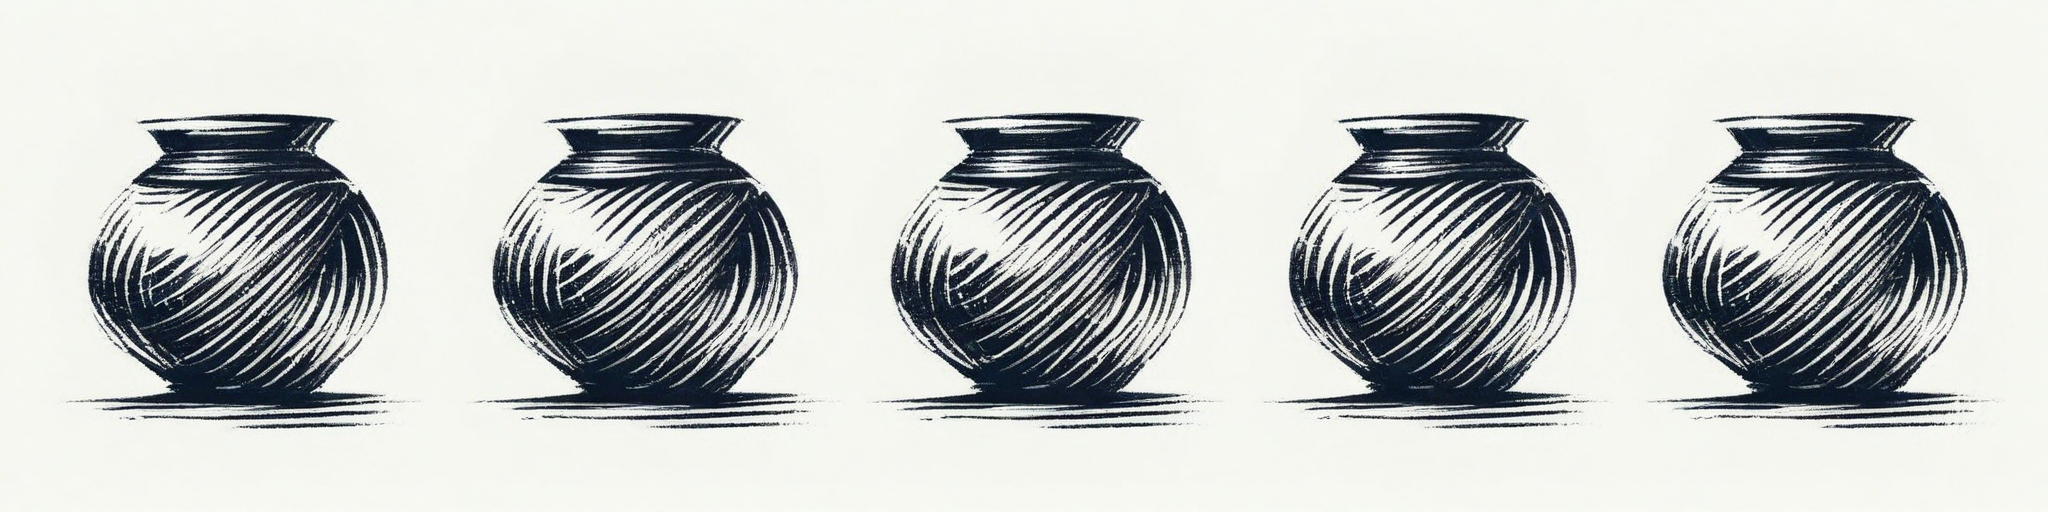
\includegraphics[width=\textwidth]{images/chapterImages/genesis_sketch_00092_.png}
\end{center}

Three rotations remaining.

The wrongstar was no longer star or disk or presence. It was everything. It filled the sky from horizon to horizon, dominating vision so completely that looking anywhere meant looking at it. The detail was overwhelming—craters and ridges and vast plains of different materials all visible on the approaching surface. Individual features larger than mountains. Topology that would reshape on impact, redistributing across the planet as ejecta and shockwave and devastating thermal pulse.

They could see their own death approaching. Could observe it with perfect clarity. Could calculate, down to the hour, when it would arrive.

The heat was beyond tolerance. Many of the older ones had already died from exposure. Their bodies lay where they fell. No one moved them. No one performed ceremony. They were already matter in transition. Already beginning their return to constituent elements. The process would accelerate dramatically in three rotations, but it had already begun.

The Pair still stood together. The weaker one had collapsed two days ago. Could no longer maintain standing position. Lay on its side, breathing shallow, consciousness fading in and out. The stronger one lay beside it. Not collapsed from weakness. Just choosing proximity. Choosing to be present for the final time rather than standing apart.

They had intertwined their necks. A position that was physically awkward, slightly uncomfortable, maintained through continuous muscular effort. They held it anyway. Physical connection until the end. Unity manifested as bodies pressed together despite the heat, despite the difficulty, despite the discomfort.

Because discomfort was temporary. Separation would be permanent. And these were the final moments when choice still mattered. When consciousness could still decide: together or alone.

They had chosen together.

\scenebreak

Aurelia had not moved from her position for seven rotations. Didn't need to move. Didn't need food or water. The body's requirements had become irrelevant. Survival for three more rotations required no special preparation. Just endurance. Just maintaining consciousness long enough to witness the final calculation resolve into physical reality.

Around her, the gathering had thinned. Many had died from the heat. Others had left—driven by instinct to return to home territories, to familiar places, to the locations where they had lived and worked. The urge to die in known territory was strong even when knowing that territory would cease to exist as recognizable form.

But thousands remained. Enough to constitute meaningful collective witness. Enough that consciousness would observe its own ending through multiple perspectives, multiple calculations, multiple understandings all converging on the same truth.

The young ones stood with family groups mostly. The females pressed against parents. The males stood close to siblings. All of them young enough that they might survive—might hide in deep caves, might endure on minimal resources, might persist through the years of darkness and cold and ecological collapse.

The one who had watched longest—the female who had created her own small pattern—stood alone. Her family group had returned to their home territory. She had chosen to stay. To witness from this optimal location rather than seek comfort of familiar surroundings.

She stood perhaps thirty body lengths from the Watcher. Close enough that acknowledgment was possible. Far enough that each maintained independent observational position. They had not interacted since the young one left the clearing. But connection existed anyway. Teacher and student, though neither had sought those roles. Pattern-creator and pattern-learner. Two minds working at vastly different depths but toward the same understanding.

The young one's survival probability was fifteen percent. Better than most. She was clever, fast, capable. If anyone from this gathering survived, she had a chance.

But fifteen percent was still mostly death probability. Still likely termination. Still the equation balancing toward extinction for this specific individual as for most specific individuals.

Aurelia ran the calculation one more time. Couldn't help calculating. Would calculate until consciousness ceased because calculation was what consciousness did.

Fifteen percent for this young one. Eight percent for the full project. Ninety-seven percent that something survived. Probabilities nested within probabilities. Individual outcomes uncertain. Aggregate results predictable. The mathematics clear even as specific manifestation remained unknown.

\scenebreak

The Daughter arrived on the gathering's periphery as the third rotation began. Aurelia hadn't expected her. Thought she had returned to her own territory with her mate and offspring. But she came anyway. Came without her family. Just herself. Choosing to spend final rotation at the witness location rather than the home territory.

She found her position—not next to the Watcher, not distant either. Close enough for presence. Far enough for independence. Aurelia acknowledged her with slight posture shift. The daughter returned the acknowledgment. No other communication passed between them.

They had worked together for years. Had calculated complementary aspects of the same problem. Had raised young who would contribute their own understanding. Had built patterns that intersected and reinforced each other.

Now they stood in final configuration. Witness position. Waiting for mathematics to manifest as physical event.

The daughter was old now. Not as old as the Watcher, but past prime. Her survival probability was six percent. Essentially zero. She would die in the impact or shortly after. Her consciousness would terminate. Her calculations would cease.

But her work would persist. The atmospheric recovery timeline she had encoded would unfold as calculated. The information she had carved and arranged and protected would guide the planet's return to equilibrium over tens of thousands of years. Her understanding would outlive her by timeframes that made individual existence meaningless.

That was what consciousness could achieve. Not physical immortality. But informational persistence. Calculation encoded in form that survived the calculator. Understanding propagating beyond the understander.

The daughter looked at the sky. At the wrongstar that now showed curvature—no longer flat but dimensionally obvious. A massive sphere approaching impact trajectory. Tumbling slowly enough that rotation was visible. Surface features moving across the field of view as it turned.

She had calculated atmospheric disruption from this impact. Had modeled thermal pulse propagation. Had determined that 94\% of atmospheric oxygen would be temporarily bound in combustion reactions. That breathing would become difficult for weeks. That many survivors of the impact itself would suffocate in the oxygen-depleted aftermath.

The mammals in their burrows would survive that phase. Would breathe slower. Would hibernate through the worst of it. Would emerge when oxygen levels recovered to find a world transformed but survivable.

She had calculated it all. Had encoded the timeline. Had ensured future consciousness would understand the recovery parameters.

Now she would experience the event she had calculated. Would observe her own predictions manifesting. Would die knowing the mathematics was correct.

That was sufficient. That was the only victory consciousness could claim: understanding what destroyed it. Calculating termination conditions with precision. Witnessing truth even when truth was extinction.

\scenebreak

Two rotations remaining.

The heat was killing everything that remained exposed. Plants were combusting spontaneously. Smaller animals were dying from hyperthermia. Even the dinosaurs showed severe stress—panting continuously, seeking any shade that still existed, bodies pushed beyond design tolerance.

Many more collapsed. The gathering was perhaps half its original size now. Those remaining were the hardiest. The most resilient. The ones with the best heat tolerance genetics. They would survive two more rotations. Would witness the impact before they died.

The Pair's weaker member had stopped breathing. Had terminated consciousness sometime during the previous rotation. The body remained where it was, pressed against its companion. The surviving member had not moved. Still maintained position. Still held the intertwined neck posture even though the other could no longer feel the contact.

Presence for the dead was meaningless. The dead didn't experience anything. Didn't benefit from proximity. Didn't care whether their body was attended or abandoned.

But the surviving one stayed anyway. Maintained contact. Chose to spend final rotation pressed against a body that no longer contained consciousness. Because connection mattered even when one half of the connection had terminated. Because the relationship had been real even if it couldn't be calculated. Because some behaviors persisted beyond their functional utility simply because they felt necessary.

Aurelia understood this. Thought of the other one who had dispersed years ago. Thought of the marked stone that indicated where his matter had been. Thought of the final positioning she had given his pattern section—maintaining his contribution, honoring his work, keeping his understanding alive even though he wasn't present to witness it persist.

She had done something similar to what the Pair's survivor was doing. Had maintained connection to consciousness that no longer existed. Had behaved as if the relationship still mattered even though one participant had terminated.

Mathematics couldn't capture this. Couldn't quantify the impulse to honor what was gone. Couldn't calculate the utility of marking a stone or maintaining a neck-intertwine position with a body that no longer felt anything.

But the behavior existed anyway. Emerged from consciousness. Persisted despite being incalculable. Mattered in ways that made no evolutionary sense but felt absolutely necessary.

Perhaps that was what would propagate forward. Not just the encoding. Not just the genetic instructions. But the tendency of consciousness to create connection. To honor what was gone. To maintain relationship beyond rational justification.

The mammals would feel it too. Would develop societies based on connection that exceeded utility. Would honor their dead. Would maintain relationship with absent partners. Would love in ways that made no survival sense but defined what being conscious meant.

That feeling wasn't in the code.

That feeling was why there was code at all.

\scenebreak

One rotation remaining.

The wrongstar's scale had become incomprehensible. It filled every direction. Looking up or east or west or south or north—everywhere was wrongstar. The world had ceased to exist. Only the approaching collision mattered. Only the final moment that was approaching with mathematical certainty.

Aurelia stood in the position she had chosen. Had not moved for ten rotations. Her body was shutting down from heat exposure. Organs failing systematically. Consciousness would terminate soon even without the impact. But she would last one more rotation. Would maintain awareness long enough to witness.

The young female was still present. Still standing. Still surviving through youth and resilience and genetic luck. She would see the impact. Would experience the shockwave. Would probably survive the initial blast. Her deep cave was only half a rotation's travel away. If she left now, she could reach it before impact. Could hide. Could maximize survival probability.

She stayed anyway. Chose witness position over survival position. Chose to observe over choosing to hide. Made the same decision the Watcher had made, the daughter had made, all of them had made: understanding mattered more than survival probability. Consciousness required witness even if witness meant death.

That was what separated consciousness from simple life. The ability to choose truth over safety. To observe what destroyed you. To calculate your own ending with precision and watch it unfold exactly as calculated.

Simple life fled. Hid. Maximized survival without understanding threat.

Consciousness stayed. Watched. Understood extinction as it approached.

That difference was what made consciousness worth encoding. Worth preserving. Worth sacrificing everything to ensure it continued in some form even if this specific form terminated.

The mammals would develop it too. Would choose truth over comfort. Would observe dangerous things because understanding mattered. Would calculate their own extinction probability and work to reduce it rather than hiding from the knowledge.

And they would succeed. Would build defenses. Would protect the planet. Would redirect the next asteroid. Would ensure consciousness persisted through the next catastrophe.

Because she had encoded the capability.

Because the plan was sound.

Because eight percent was sufficient to try.

\scenebreak

The final hour approached.

The wrongstar's curvature had flattened. No longer appeared spherical. Just an infinite plane descending from above. Filling the entire sky. Pressing down like weight. The feeling of it was physical even before it arrived. The pressure of mass approaching collision. The inevitability of impact.

They could see the impact point now—a location on the wrongstar's surface that remained stationary while everything else rotated around it. The point that would strike first. The location where all the kinetic energy would begin converting to heat and shockwave and global destruction.

The calculations had predicted this point. Had identified it years ago. Had determined exact impact location down to a few miles of error. The observation confirmed the calculation. The mathematics was perfect. The trajectory was exactly as predicted.

They had been right about everything.

The mammals were positioned correctly.

The encoding was complete.

The timeline would unfold as calculated.

And they would die knowing this. Would terminate with certainty that the work was sound even if the outcome remained probabilistic.

That certainty was all consciousness could claim. Understanding without survival. Truth without continuation. Knowledge that existed for one moment before dispersing with the knower.

Aurelia looked at the gathering one final time. Thousands had become hundreds. Hundreds were becoming dozens as the heat killed systematically. But enough remained. Enough witnesses to confirm the calculation. Enough consciousness to observe truth.

The daughter stood in her position. Still present. Still conscious. She would not survive the shockwave. She had known this. Had come anyway.

The young female stood alone. Still living. Still capable. Still choosing witness over survival. She might persist. Might make it to her cave. Might endure through the years of darkness. Might become one of the fifteen percent. Might carry forward some fragment of understanding.

The Pair had fully dispersed now. Both bodies still. Both consciousness terminated. But they remained together. Matter pressed against matter. The relationship persisting in physical form even though the participants had ceased.

She had done the same for the other one. Had marked his location. Had maintained his pattern. Had kept his contribution present even though he wasn't.

Connection persisted beyond consciousness. That was what made it real.

The young ones who had learned at her clearing—most were gone now. Had returned to territories. Had chosen different witness locations or different end positions. But the learning had happened. The understanding had transferred. The pattern had propagated through observation and correction and the patient process of minds showing other minds what was possible.

She stood where she had calculated she would stand. The northern plateau. Optimal witness position. Clear sightlines. Stable geology. Everything exactly as mathematics predicted.

The wrongstar descended.

Time measured in minutes now. Not rotations. Not hours. Minutes.

She had calculated across 65 million years. Had planned for timeframes that made geological epochs look brief. Had encoded instructions that would unfold across three million generations.

And now it came down to minutes.

The last minutes of this consciousness. This specific pattern of calculation and observation and understanding. This particular manifestation of universe experiencing itself.

The end was approaching.

But the mathematics was sound.

The plan would unfold.

And consciousness would persist—not this consciousness, but consciousness. The pattern that recognized itself. That calculated its own continuation. That chose to ensure something survived even when survival for itself was impossible.

That was sufficient.

That was everything.

The wrongstar was so close now that individual features on the surface were enormous. Mountain-sized irregularities. Plains the size of continents. All of it approaching at velocity that made the numbers abstract even as the reality was devastatingly concrete.

Aurelia checked the calculation one final time.

Everything was positioned correctly.

The mammals would survive.

The encoding would persist.

The timeline would begin.

Sixty-five million years.

Three million generations.

Eight percent chance.

The equation was about to balance.


\chapter{The Impact}
\label{ch:15}



\begin{center}
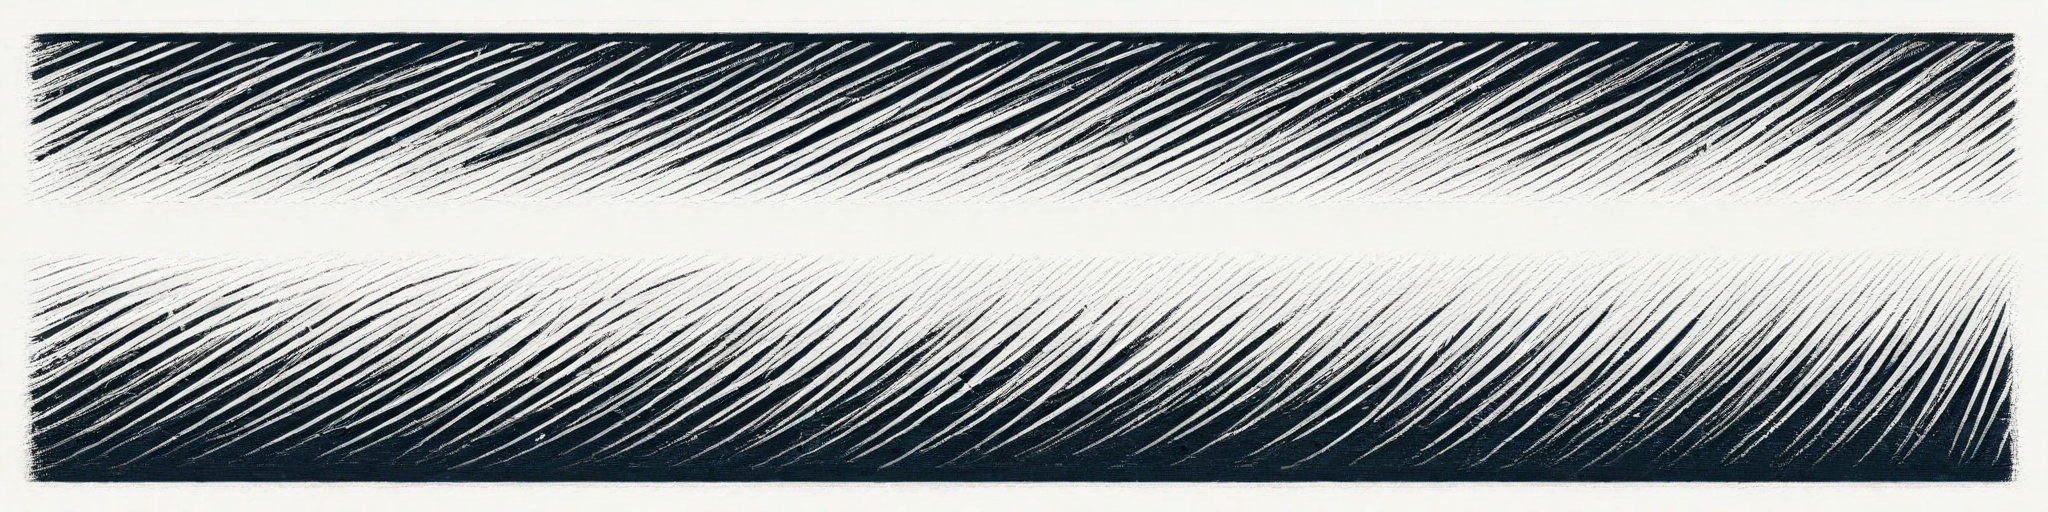
\includegraphics[width=\textwidth]{images/chapterImages/genesis_sketch_00098_.png}
\end{center}

The light came first.

Not from the wrongstar itself but from its interaction with the upper atmosphere. Friction. Compression. Air molecules forced aside at velocities they were never designed to accommodate. The energy of that displacement converting to heat. To light. To radiation across the spectrum.

The sky ignited.

Not gradually. Instantaneously. The entire visible atmosphere became luminous. Brighter than day. Brighter than anything that had existed before. Light that carried heat. Light that was heat. Light that burned.

Aurelia's final thought was observation: the calculations were correct.

The trajectory matched prediction within error margins. The atmospheric interaction was proceeding as modeled. The angle of approach was optimal for maximum global distribution of ejecta. Everything was exactly as the mathematics had determined it would be.

The encoding would survive. The mammals were positioned correctly. The timeline would unfold.

Eight percent.

Sufficient.

The light intensified beyond the capacity of eyes to process. Vision ceased to function. Became irrelevant. The sensory input was just pain signal—too bright, too hot, tissue damage occurring at cellular level.

But consciousness persisted for another moment. Long enough to feel satisfaction. Not happiness. Not peace. Just the mathematical certainty that the equation was balancing exactly as calculated.

The work was complete.

\scenebreak

The sound arrived.

Not heard—felt. A pressure wave moving through air and ground simultaneously. Frequency so low it was more earthquake than noise. The planet itself transmitting the shock of collision. Every molecule between impact point and witness location suddenly displaced, all trying to occupy the space their neighbors had just vacated, creating a cascade of compression that propagated at supersonic velocity.

The gathering scattered like leaves. Bodies lifted and thrown by wind that shouldn't exist. By pressure differential that exceeded any biological resistance. They tumbled through air that was no longer air but plasma. Super-heated. Ionized. Carrying enough energy to flash-cook tissue on contact.

The daughter's consciousness terminated mid-flight. Instant. Clean. No suffering. Just function ceasing as thermal energy exceeded cellular tolerance.

The young female made it three seconds longer. Landed. Tried to run toward her cave half a rotation away. The ground was moving too violently to permit running. She fell. The heat intensified. Her consciousness fragmented—pain signals overwhelming processing capacity. Then nothing. Termination.

The Pair's bodies ignited where they lay. The intertwined necks maintained their position briefly as matter converted to combustion. Then even the physical connection failed. Dispersed. Returned to constituent elements.

Aurelia's body ceased functioning. Organs shut down. Neural activity terminated. The vast cathedral of calculation that had existed behind her eyes—the timelines and probability curves and encoded instructions spanning 65 million years—all of it vanished in an instant.

Consciousness ended.

The universe continued experiencing itself, but not through her.

\scenebreak

The wrongstar struck the planet.

Ten kilometers of nickel-iron traveling at 70,000 kilometers per hour met continental crust three kilometers thick. The physics was straightforward even if the scale was incomprehensible. Kinetic energy converted to heat. Matter compressed beyond tolerance. Bedrock behaving like fluid. Shockwave propagating spherically.

The impact crater formed in seconds. Thirty kilometers deep. Two hundred kilometers across. The ejecta plume rose immediately—millions of tons of vaporized rock and impactor material thrown into ballistic arcs that would carry them halfway around the planet.

The heat pulse ignited everything flammable within a thousand kilometers. Forests became firestorms. Animals became ash. The atmosphere itself burned where oxygen concentration was sufficient.

The shockwave propagated globally. Circles expanding from impact point. When it reached the northern plateau—already empty of witnesses, already cleared of consciousness that could observe it—it scoured the surface clean. The stone patterns scattered. The careful arrangements destroyed. The physical encoding erased.

But the information had already been transferred. Already existed in the genetics of protected populations. Already resided in forty-three locations where small mammals huddled in deep burrows and waited for the shaking to stop.

\scenebreak

In a cave system beneath the western mountains, the tool-using population experienced the impact as darkness and terror and confusion. The ground shook. Rocks fell. Some individuals died crushed. Others injured. The group pressed together in the deepest chambers and waited.

They had no understanding of what was happening. No framework for comprehending planetary-scale catastrophe. Just instinct: hide, wait, survive.

The temperature in the burrow rose but not beyond tolerance. The air grew thin but remained breathable. The shaking eventually stopped. The darkness continued.

They waited.

In their genes, encoded sequences that had been selected for over years waited too. Dormant. Inactive. But present. Ready to express when environmental conditions triggered activation. Ready to unfold across timescales these small creatures couldn't imagine.

Tool use: present and active.
Fire control: dormant, awaiting activation at population density threshold 200,000 years from now.
Agriculture: dormant, awaiting climate stabilization 10,000 years from now.
Language: dormant, awaiting vocal structure evolution.
Mathematics: dormant, awaiting neural development.

On and on. Twenty-seven major thresholds. Hundreds of minor ones. All encoded. All waiting. All positioned in the genome where they would activate on schedule if evolution proceeded along calculated trajectories.

If the population survived. If the traits propagated. If the timeline held.

If.

The tool-users waited in darkness. Some died from injuries sustained in the shaking. Others from stress. The survivors huddled together and waited for the world to make sense again.

It wouldn't make sense for a long time. The impact winter was just beginning. The darkness would persist for months. The cold would intensify. The resources would become scarce. Many would die. Most, probably.

But some would survive. The mathematics said so. The calculations were sound. Eight percent for full success. Ninety-seven percent that something persisted.

The mammals waited. And the code they carried waited with them. Patient. Dormant. Ready.

\scenebreak

The planet convulsed. Volcanism triggered globally by the shockwave's seismic energy. Tsunamis propagating across every ocean. The atmosphere choking with particulate matter. Sunlight blocked. Temperature plummeting. The greenhouse effect reversing to ice house in a matter of weeks.

Ninety-nine point seven percent of large organisms died within the first year. Ninety-four percent of all species extinct within ten years. The world transformed. The climate collapsed. The ecosystems simplified to extremophile survivors and small creatures that could hide and wait and endure.

The dinosaurs vanished completely. Every individual. Every population. Every remnant of the consciousness that had calculated and planned and encoded the future. Gone. Dispersed. Returned to the elements from which they had briefly been organized into pattern.

The mammals endured. Not all of them. Not even most. But enough. In forty-three locations, populations survived the first year. By the second year, thirty-seven populations remained. By the fifth year, twenty-eight. By the tenth year, nineteen.

Nineteen lineages carrying encoded traits. Nineteen populations positioned across the recovering landscape. Nineteen points of potential for the timeline to unfold.

It was enough.

Barely. Just barely. But enough.

\scenebreak

Sixty-five million years later, a woman named Sarah Chen stared at a genetic sequence on a computer screen and felt understanding dawn.

The dinosaurs hadn't just existed. They had planned. Had calculated. Had encoded.

Had loved their world enough to ensure something survived even though they couldn't.

The traits weren't random. The cognitive capabilities weren't evolutionary accidents. Tool use and fire control and agriculture and language and mathematics and astronomy—all programmed. All scheduled. All activated according to a timeline designed before humanity existed.

We were the execution of their code.

The inheritors of a gift we never knew we'd received.

And somewhere in that code, somewhere in the 65-million-year plan that had unfolded exactly as calculated, was an imperative: protect this world. Build the defense grid. Redirect the next asteroid. Ensure consciousness persists.

Ensure something survives.

Pass it forward.

The cycle continues.

\scenebreak

On the northern plateau, long empty of witnesses, wind scattered the last stones. Rain eroded the final configurations. The pattern that had existed dissolved into randomness. The mathematics returned to the landscape from which it had been briefly extracted.

But the understanding persisted. Encoded in living flesh. Written in DNA. Waiting to unfold across geological time.

Aurelia's consciousness had terminated. Her body had dispersed. Her individual existence was complete.

But her work continued. Her calculations propagated forward. Her contribution to collective understanding existed independent of her presence.

The equation had balanced.

Life equaled matter plus pattern plus time.

Consciousness equaled life plus observation plus calculation.

Persistence equaled consciousness plus encoding plus sacrifice.

The variables resolved. The mathematics completed. The timeline began its long, patient unfold toward an uncertain future that was nevertheless calculated with precision.

Eight percent.

Sufficient.

The equation balanced.

\scenebreak

**END OF PART ONE**



% ============================================================
% PART TWO: THE INHERITORS
% ============================================================

\part{The Inheritors}
\label{part:inheritors}

\begin{center}
\itshape
Present Day
\end{center}

\cleardoublepage

% Import Part Two Chapters
\chapter{Chapter 16}
\label{ch:16}

\# PART TWO: THE INHERITORS

\# Chapter 16: The Sequence

\begin{center}
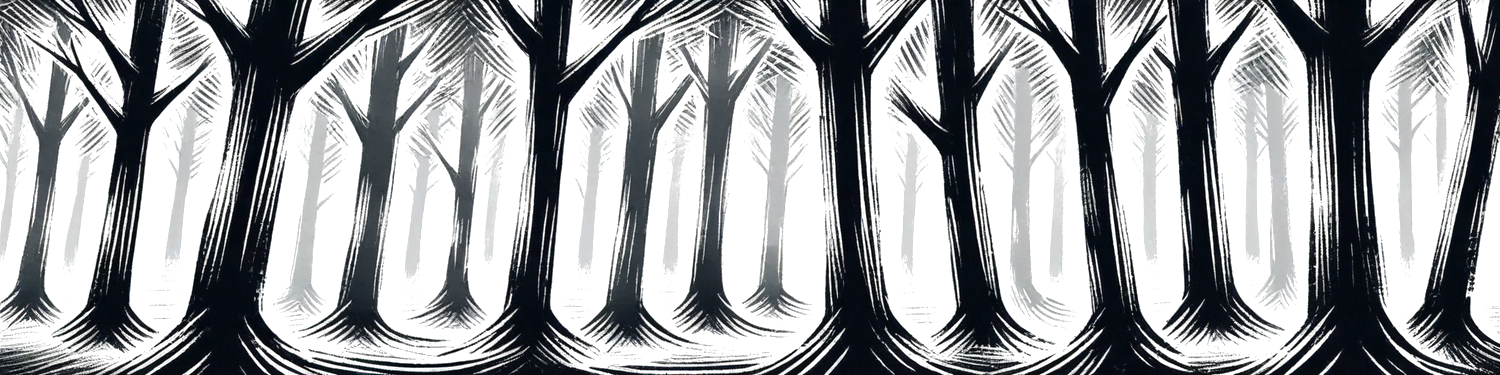
\includegraphics[width=\textwidth]{images/chapterImages/genesis_sketch_00103_.png}
\end{center}

2:17 AM. Sarah Chen's eyes burned from staring at the screen. She should have gone home three hours ago. Should have been in bed four hours ago. Should have been a functional parent who made it to her daughter's school play last week instead of the geneticist who sent apologetic texts and promised to make it up somehow.

The lab was silent except for the hum of equipment and the occasional click of her keyboard. Everyone else had gone home. Had lives. Had families. Had priorities that didn't include staring at genetic sequences until their vision blurred.

She reached for her coffee. It was cold. She drank it anyway.

The sequence on her screen was wrong. Not corrupted data wrong. Not sequencing error wrong. Wrong in a way that made no sense if you believed in 3.8 billion years of messy, random, undirected evolution.

It was too regular.

She had been analyzing "junk DNA"—the 98\% of the human genome that didn't code for proteins. The sections everyone assumed were evolutionary detritus. Leftover fragments from our genetic history. Meaningless noise accumulated over billions of years.

Except this section wasn't noise.

She highlighted a 2,000 base pair segment and ran correlation analysis. The pattern recognition software—designed originally for SETI, for finding signals in cosmic noise—lit up like Christmas.

Mathematical relationships. Fibonacci sequences. Prime number spacing. Patterns that occurred with frequency far beyond what randomness could produce.

She sat back. Rubbed her eyes. Ran the analysis again because maybe she was just tired. Maybe her caffeine-deprived brain was seeing patterns where none existed.

The results came back identical.

"Fuck," she said to the empty lab.

Her phone buzzed. Text from her ex-husband: *Maya's asking about the play. What should I tell her?*

Sarah stared at the message. Guilt twisted in her stomach. She'd missed another thing. Another moment. Another chance to be the parent Maya deserved instead of the obsessive researcher who couldn't let anything go.

She typed: *Tell her I'm sorry. Tell her I'll make it up to her.*

Delete. Try again: *I'll call her in the morning.*

Delete. Finally: *Can you keep her an extra few days? Important work thing.*

Send before she could change her mind.

The phone buzzed immediately. *Sarah, you can't keep—*

She turned the phone face-down and returned to the screen.

The pattern was still there. Still impossible. Still undeniable.

\scenebreak

She ran expanded analysis. Pulled the same genomic region from archived sequences. Chimpanzees. Gorillas. Orangutans. All great apes. Then further: Old World monkeys. New World monkeys. Lemurs.

The pattern appeared in all of them. Identical. Absolutely identical across 60 million years of divergent evolution.

That shouldn't happen. Random mutation should have scrambled it. Should have introduced errors. Should have made the pattern degrade with each generation, each split, each million years of separate evolution.

But it was identical. Perfectly preserved. As if protected. As if... selected for.

No. That was insane. You couldn't select for junk DNA. It didn't do anything. It didn't code for any survival advantage. Natural selection only worked on traits that affected fitness. This was just meaningless base pairs sitting between functional genes.

Except.

She pulled up correlation databases. Ran the sequence against every known genetic marker. Cross-referenced with neural development, cognitive capability, brain structure variation.

The results came back and Sarah's hands started shaking.

The pattern correlated—strongly, undeniably—with specific brain structures. The regions that enabled tool use. The neural pathways that linked visual processing to fine motor control. The cognitive architecture that allowed humans to pick up a stick and imagine using it as an extension of their arm.

Tool use.

This "junk DNA" sequence corresponded exactly to the genetic foundation of tool use capability.

Sarah pulled up her notes from her doctoral thesis. She'd studied the evolution of cognitive capabilities. Had documented the archaeological timeline. Stone tools appearing 2.6 million years ago. Right when brain size started increasing. Right when we diverged from our last common ancestor with chimps who didn't use tools systematically.

She ran dating analysis on when this genetic sequence would have "activated"—when its expression would have increased. When whatever regulatory mechanism controlled it would have turned on.

2.6 million years ago.

Plus or minus 50,000 years.

"No," she said out loud. "No, that's coincidence. Has to be."

She pulled up the next segment of the pattern. Ran the same analysis. This one correlated with heat resistance in hand tissue. With reduced fear response to fire. With cognitive structures that enabled risk assessment of controlled combustion.

Dating analysis: 400,000 years ago.

Archaeological record for controlled fire: 400,000 years ago.

Sarah stood up. Paced to the window. The campus was dark. Empty parking lots. A few security lights. Normal world where genetics was random and evolution was undirected and coincidences were just coincidences.

She went back to the computer.

Pulled up the third segment. Already knowing. Already certain. Already terrified of what she was going to find.

Agricultural timing. Seasonal awareness. The cognitive capacity for long-term resource planning. The ability to delay gratification, to plant seeds you wouldn't harvest for months, to think beyond immediate survival.

Dating: 12,000 years ago.

Agricultural revolution: 12,000 years ago.

She kept going. Couldn't stop now. Fourth segment. Fifth. Tenth. Twentieth.

Every major cognitive threshold in human evolution. Every breakthrough that separated us from other primates. Every capability that built civilization.

All of it was there. In our junk DNA. Perfectly preserved. Activated on schedule. One after another after another like someone had programmed the sequence. Like someone had written the code for human development and set timers for when each capability should unlock.

Someone.

Something.

Sarah looked at the timestamp on the genetic sequence. The software estimated when this pattern had been inserted into the mammalian genome. When it first appeared in our evolutionary lineage.

65 million years ago.

Plus or minus 2 million years.

The Cretaceous-Paleogene boundary. The K-T extinction. The asteroid that killed the dinosaurs.

This sequence appeared exactly when the dinosaurs disappeared.

Her phone buzzed again. She ignored it. Pulled up every analysis tool she had. Ran verification after verification. Checked for equipment error. Checked for software bugs. Checked for any possible explanation that didn't involve what her data was screaming at her.

Nothing. The pattern was real. The correlations were solid. The timeline was precise.

Someone had programmed human evolution 65 million years ago.

And they had done it with such precision that every major breakthrough in human cognitive development corresponded to a scheduled activation in our junk DNA.

We weren't the authors of our own progress.

We were executing code.

The phone buzzed again. Sarah picked it up with shaking hands. Another text from her ex: *Sarah, Maya is crying. She's asking why you're never there. I need to tell her something.*

Sarah stared at the text. At her daughter's pain reduced to pixels on a screen. At the latest evidence that she was failing at being human while succeeding at being a scientist.

She looked back at the computer. At the pattern that suggested humanity itself was a program. That every choice, every breakthrough, every achievement was scheduled activation of pre-written code.

If that was true—if we were just executing instructions written 65 million years ago—then was anything real? Did any choice matter? Was she actually deciding to prioritize work over Maya, or was that decision just another subroutine running its course?

She typed back: *Tell her I'm doing this for her. For everyone. Tell her... tell her I'm sorry.*

Send.

Immediately regretted it. Wanted to take it back. Wanted to leave right now, drive to her ex's house, wake Maya up and hold her and be the parent she should have been all along.

But the data was still on the screen. Still impossible. Still real. Still requiring analysis and verification and investigation and all the things that meant not leaving, not going home, not being there.

Again.

Her phone buzzed one more time. She expected another message from her ex. Disappointed anger. Justified frustration.

But it was Maya. A text in her seven-year-old's careful, laborious typing: *miss you mommy*

Three words. No punctuation. The effort it must have taken to find each letter on the keyboard.

Sarah's vision blurred. She wiped her eyes angrily. Scientists didn't cry. Scientists analyzed data objectively. Scientists looked at evidence without emotional compromise.

She looked at the genetic sequence. At the pattern that might mean humanity was programmed. At the work that kept pulling her away from her daughter. At the impossible choice between understanding truth and being present for the person who needed her.

And she chose truth.

Again.

She texted back: *Miss you too baby. I'll see you soon. I promise.*

Lie. She didn't know when she'd see Maya again. Didn't know how long this analysis would take. Didn't know how you told your daughter that you missed bedtime and the school play and every important moment because you were discovering that human free will might be an illusion.

She turned the phone off completely. Couldn't handle more interruptions. Couldn't handle more evidence of her failures as a mother while she documented evidence of humanity's failure to be autonomous.

The lab was silent again. Just her and the data and the growing certainty that everything she thought she understood about being human was wrong.

The sequence sat on her screen. Regular. Purposeful. Impossible.

And somewhere in the code was another segment. Another activation sequence. Another scheduled breakthrough.

Still dormant.

Still waiting.

Sarah pulled up the analysis of the inactive section. Started running dating projections. When would this one activate? What capability would it unlock? What was coming next in the program that someone had written for humanity 65 million years ago?

The projection came back: 0-5 years. Margin of error too large for precision but the window was close. Very close.

This generation. Maybe her generation. Maybe Maya's.

Some new capability was about to activate. Some new threshold was approaching.

Sarah leaned forward and started documenting everything. Taking screenshots. Exporting data. Creating a record that other researchers could verify. Because this was too big for one scientist working alone at 2 AM. Too big for one lab. Too big for any individual to carry.

But for tonight—for these hours—it was hers. She was the first. The only one who knew.

Humanity was programmed.

And the program was still running.

Outside the window, the campus began to lighten. Dawn approaching. Time passing while she sat frozen in revelation.

Her coffee had long since gone cold. She didn't notice. Didn't care. Just kept working. Kept analyzing. Kept documenting the evidence that humanity was executing a 65-million-year-old code written by minds we never knew existed.

The phone stayed off. Maya would wake up soon. Would eat breakfast without her mother. Would go to school without her mother. Would live another day in which her mother chose work over presence.

Sarah felt the guilt. Acknowledged it. Kept working anyway.

Because if this was real—if humanity was programmed—then she needed to understand it. Needed to document it. Needed to know what came next.

Even if it meant missing everything else.

Even if it meant failing at being human while discovering that being human meant executing code.

The equation had balanced 65 million years ago.

Now it was beginning to unfold.

And Sarah Chen was the first to notice.

The first to understand.

The first to bear the weight of knowledge that changed everything.

She saved her work. Backed it up three times. Then opened a new analysis window and started on the next section of the sequence.

There would be time for Maya later. Time to make up for missed moments. Time to be the parent she should have been.

But right now, there was only this. Only the pattern. Only the truth.

Only the growing certainty that humanity's story was someone else's plan.

And that plan was still unfolding.


\chapter{The Correlation}
\label{ch:17}



\begin{center}
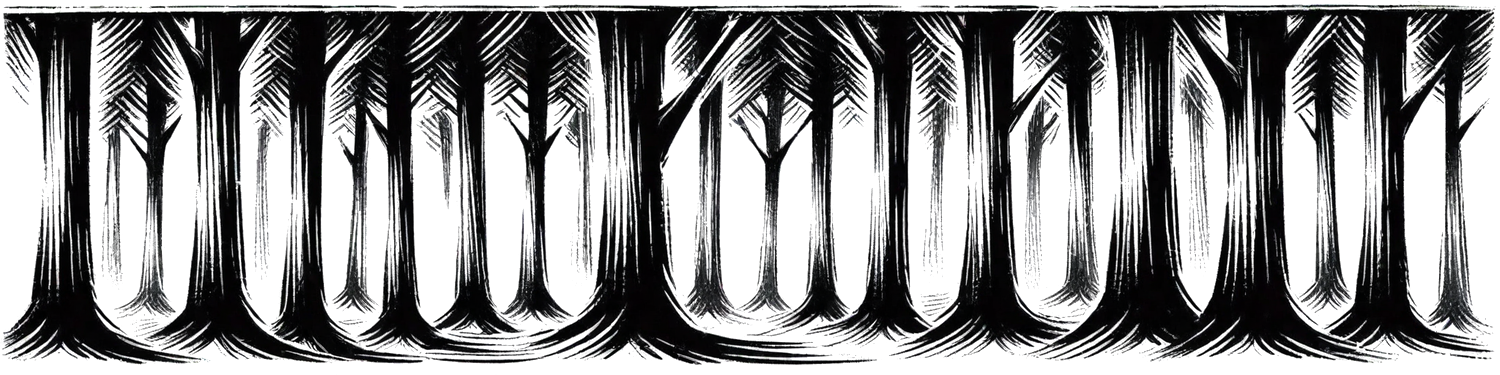
\includegraphics[width=\textwidth]{images/chapterImages/genesis_sketch_00104_.png}
\end{center}

Sarah didn't go home. Didn't sleep. By 9 AM she had consumed four more cups of coffee and documented seventeen distinct activation sequences in the human genome. By noon she had cross-referenced all of them against archaeological and anthropological data. By 3 PM she was staring at a timeline that made her question whether reality was real.

Every sequence. Every single one. Correlated with a major evolutionary threshold.

She had created a visualization—a simple chart with two timelines. Archaeological record on top. Genetic activations on bottom. The lines matched so perfectly it looked fabricated.

Tool use: 2.6 million years ago. Both timelines.
Fire control: 400,000 years ago. Both timelines.
Symbolic thought: 100,000 years ago. Both timelines.
Agriculture: 12,000 years ago. Both timelines.
Writing: 5,000 years ago. Both timelines.
Mathematics: 2,500 years ago. Both timelines.

On and on. Every threshold. Every breakthrough. Every capability that made humans human.

All of it was in the code. Scheduled. Timed. Activated precisely when needed.

Her office phone rang. She ignored it. It rang again. Again. Finally she picked up.

"Dr. Chen, this is Janet from the Dean's office. We've been trying to reach you. You missed your lecture this morning and—"

"I quit," Sarah said.

Silence on the other end.

"I'm sorry, what?"

"I quit. I'm resigning. Effective immediately. Send me whatever paperwork. I'll sign it."

"Dr. Chen, you can't just—"

Sarah hung up. Unplugged the phone from the wall. Went back to her computer.

She needed to talk to someone. Needed verification. Needed another set of eyes on this data before she lost her mind completely.

James Wei. Archaeologist. They'd collaborated on a paper five years ago about cognitive evolution. He was solid. Careful. Skeptical in the good way—demanded evidence before accepting claims.

She pulled up his contact info and called his cell.

"James Wei."

"James, it's Sarah Chen. I need you to look at something. Right now. Today. Can you come to my lab?"

"Sarah? I'm in the middle of—"

"I found something in the human genome. Something that correlates with your archaeological timeline. Perfectly. Impossibly perfectly."

Pause. "What kind of correlation?"

"Just come. Please. I can't explain over the phone. You need to see the data."

Another pause. Longer. "Give me two hours."

\scenebreak

James arrived in ninety minutes. He was tall, thin, perpetually rumpled in the way academics who didn't care about appearance often were. He had his laptop bag and what looked like half his office in a cardboard box.

"Okay," he said without preamble. "Show me."

Sarah pulled up the visualization. The two timelines. The perfect correlation.

James stared at it for a long time. Too long. Sarah was about to prompt him when he finally spoke.

"This is fake."

"It's not."

"Then your data is corrupted."

"It's not."

"Then your analysis is wrong."

"It's not."

He turned to look at her. Really look at her. "Sarah, when was the last time you slept?"

"Show me I'm wrong," she said. "Show me any error in the methodology. Any contamination in the data. Any mistake in the correlation analysis. Show me and I'll admit I'm wrong."

James sat down. Started going through her documentation. He worked in silence for three hours, checking every calculation, every correlation, every cross-reference. Sarah made more coffee and watched him work and tried not to think about Maya or her resigned position or the fact that her entire life was currently imploding.

Finally, James sat back. Rubbed his face. Looked at the timeline again.

"Fuck," he said quietly.

"Yeah."

"This is... Sarah, do you understand what you're suggesting?"

"That human evolution was programmed. That every major breakthrough in our development was scheduled. That we're not the authors of our own progress."

"That's insane."

"Show me where the data is wrong."

He couldn't. She could see him trying. See him looking for any way to dismiss it. Any explanation that didn't require accepting the impossible.

"Newton and Leibniz," he said finally.

"What?"

"Newton and Leibniz both invented calculus independently. Within years of each other. Different countries. No communication. How do you explain that?"

Sarah pulled up another data set she'd been analyzing. "Activation wave. Look at the timeline for advanced mathematical reasoning capability. It doesn't activate uniformly across the population. It activates in waves. First a few individuals. Then more. Then widespread. Newton and Leibniz both got the first wave. They weren't geniuses who happened to discover the same thing. They were both activated at the same time."

James stared at her. "You're telling me genius is just... scheduled?"

"I'm telling you the capability for genius is scheduled. What individuals do with it might be up to them. But the capacity itself? The cognitive architecture that makes advanced mathematics possible? That activates on a timeline. And that timeline was set 65 million years ago."

"By who?"

"That's the question, isn't it?"

James stood up. Paced to the window. Looked out at the campus. Normal people doing normal things. Students heading to class. Professors discussing research. The regular world where evolution was random and humanity was self-made.

"I need to show you something," he said. "I've been documenting simultaneous discoveries. It started as just an interesting pattern I noticed. Darwin and Wallace both proposing natural selection at the same time. Kelvin and Joule both working on thermodynamics. Helmholtz and Mayer both discovering energy conservation. I thought it was just convergent thinking. Same problems, similar solutions."

He pulled files from his cardboard box. Papers. Notes. Timelines of his own.

"But I kept finding more. Every major innovation has multiple independent discoverers. Not just two. Sometimes five. Sometimes ten. All working on the same problem. All arriving at the same solution. All within the same narrow time window."

He spread the papers across Sarah's desk. "I thought it was coincidence. Or something about the human condition—we're ready for certain ideas at certain times. Cultural readiness. Technological foundation. That kind of thing."

Sarah was already pulling up her genetic timeline. Cross-referencing. The activation waves. The periods when certain capabilities expressed more strongly across populations.

"It's not cultural readiness," she said slowly. "It's activation waves. Look—the steam engine. Multiple inventors across Europe within twenty years. Right here—mechanical engineering capability activating. Widespread expression."

"The telephone. Bell and Gray filed patents on the same day."

"Communication technology activation. Right here in the sequence."

"The internet. Multiple research groups independently—"

"Information processing architecture. Activated thirty years ago. Widespread expression last decade."

They looked at each other across the desk covered in papers and genetic printouts and timelines that all told the same impossible story.

"Someone programmed human development," James said. It wasn't a question anymore.

"Sixty-five million years ago."

"The K-T extinction."

"Exactly when the dinosaurs died."

Long silence. Outside, a bird landed on the window ledge. Ordinary. Normal. Oblivious to the revelation happening inside.

"Why?" James asked finally. "Why would anyone—why would anything—program human evolution? What's the purpose?"

Sarah pulled up the last section of the genetic sequence. The one that was still dormant. Still waiting to activate.

"I don't know yet. But there's one more threshold coming. And I think when we figure out what it's for, we'll understand the whole thing."

James leaned forward to look at the sequence. "When does it activate?"

"Soon. Within five years. Maybe sooner."

"What does it do?"

"I don't know. The correlations are complicated. It touches multiple systems. Neural structures. Sensory processing. Something to do with spatial reasoning and physics comprehension and..." She trailed off, staring at the data.

"What?"

"Oh god. James, I think this is engineering capability. Advanced engineering. Planetary-scale engineering."

"For what?"

Sarah pulled up comparative analysis. Cross-referenced with astronomical data. Let the pattern recognition software run its course.

The results came back and Sarah's blood went cold.

"Asteroid defense," she whispered. "James, this capability is for building asteroid defense systems."

They stared at the screen in silence.

Finally James said, "There's someone you need to meet. Engineer. Marcus Chen—no relation to you, I assume?"

"No."

"He's been working on satellite systems. Some kind of gravitational anchor network. Been obsessed with it for months. Says he can't explain where the ideas are coming from. Just that he knows they're correct. Knows they'll work."

Sarah's hands were shaking again. "When did he start this work?"

"Six months ago. Sudden onset. Said he woke up one morning and just... knew how to build it."

"He's activated," Sarah said. "He's one of the first. The engineering capability is activating and he's expressing it."

"Sarah, if you're right—if this is all real—we need to tell people. We need to—"

"Tell them what? That free will is an illusion? That every achievement humanity has ever claimed is just scheduled activation of pre-written code? That we're not the authors of our own story?" She laughed without humor. "How do you think that goes over?"

"But if there's another activation coming—if people are about to start building asteroid defenses—"

"Then maybe we need to understand it first. Before we announce to the world that humanity is a program."

James sat down heavily. "I need a drink."

"It's 3 PM."

"I need several drinks."

Sarah's phone—her personal cell, sitting face-down on the desk—buzzed. And buzzed. And buzzed. She'd turned it back on at some point. Messages flooding in. Her ex. The school. Probably her department head about the resignation.

She picked it up. Seventeen messages. Most from her ex. Three from a number she didn't recognize. She opened those first.

*Dr. Chen, this is Principal Morrison from Maya's school. We need to speak with you about your daughter. Please call as soon as possible.*

*Dr. Chen, this is urgent. Maya had an incident today. She's fine but we need you to come in.*

*Dr. Chen, your ex-husband picked Maya up. Please contact us to schedule a meeting about her behavior.*

Sarah's stomach dropped. She dialed the school. Got the principal's voicemail. Tried her ex.

He answered on the first ring. "Jesus Christ, Sarah, where have you been?"

"What happened? Is Maya okay?"

"She's fine. Physically. But she tried to run away from school. Got all the way to the street before a teacher caught her. Said she was trying to come find you."

The guilt hit like a physical blow. "I'm coming. Right now. I'm—"

"Don't. She's asleep. Finally. After crying for two hours. The school counselor says she's processing abandonment. Apparently you've been 'too busy' for her lately."

"I'm working on something important. I can't—"

"More important than your daughter?"

Yes, Sarah wanted to say. This is bigger than one child. This is the nature of humanity. This is everything we thought we were turning out to be a lie.

But she couldn't say that. Couldn't explain. Couldn't justify choosing cosmic truth over maternal presence.

"I'll come tomorrow," she said.

"Sarah—"

She hung up. Put the phone down. Looked at James, who was very deliberately studying the timeline and not making eye contact.

"I'm a terrible mother," she said.

"I don't have kids. Can't judge."

"You're judging."

"Little bit, yeah."

Sarah laughed. Nearly hysterical. Nearly crying. "My daughter tried to run away to find me and I'm here proving that humanity is programmed. What does that say about me?"

"That you're human," James said. "That you're doing what you were designed to do. Following the compulsion to understand. To analyze. To discover." He paused. "Or maybe you're just using work to avoid dealing with your failures as a parent. I'm an archaeologist, not a therapist."

"Wow. Thanks."

"You asked."

Sarah looked at the timeline again. At the proof that humanity was executing code. At the evidence that every choice might be predetermined. At the possibility that her obsession with work and her failures with Maya were both just subroutines running their course.

"If we're programmed," she said slowly, "then am I even choosing to be a bad parent? Or is that just part of my coding?"

"Does it matter?"

"Of course it matters. If I don't have free will, then I can't be blamed for my failures. But I also can't be credited with my successes. Nothing means anything."

James shook his head. "You're a geneticist. You know genes aren't destiny. They're tendency. Probability. The code gives you capacity—what you do with it is still yours."

"Is it?"

"I don't know, Sarah. I study dead civilizations. Not philosophy."

They sat in silence. The timeline on the screen. The evidence of programming. The impossible truth that changed everything.

"I need to meet him," Sarah said finally. "Marcus Chen. The engineer who's building asteroid defenses without knowing why. I need to understand what's happening to him."

"I'll set it up."

"And we need more people. We can't verify this alone. We need other geneticists. Other experts. We need a team."

"Agreed. But carefully. If this gets out before we understand it—"

"Panic. Existential crisis. Collapse of every religious and philosophical framework humanity has built."

"Basically."

Sarah pulled up her email. Started drafting messages to researchers she trusted. Carefully worded. Vague about the specifics. Just enough to get them curious.

Her phone buzzed again. Another message from her ex: *Maya keeps asking why you don't love her anymore. What should I tell her?*

Sarah stared at the message. At her daughter's pain reduced to a question she didn't know how to answer.

*Tell her I do love her,* she typed. *Tell her I'm trying to understand something important. Tell her I'll be there soon.*

All lies. She did love Maya. But clearly not enough to choose her over this work. Not enough to prioritize presence over discovery. Not enough to be the parent Maya needed.

And she had no idea when she'd be "there soon." This work had just begun. The implications were vast. The investigation would take months. Years, maybe.

She sent the message anyway. Added to the pile of promises she probably wouldn't keep.

Then she turned back to the computer. To the timeline. To the evidence that humanity was executing a program written before humans existed.

To the growing certainty that she was doing exactly what she was designed to do, even if it meant failing at everything else.

The equation was unfolding.

And Sarah Chen was one of the first to see it happen.

Whether she chose to investigate or was compelled to investigate didn't matter.

Either way, she couldn't stop.

The code was running.

And she was running with it.


\chapter{The Historian}
\label{ch:18}


Marcus Chen lived in a warehouse he'd converted to a workshop. When James and Sarah arrived, they found him surrounded by equipment that looked half-finished and entirely insane—metal frameworks, circuit boards, holographic projections, calculations covering every available wall surface.

He was in his early forties, Asian-American, with hair that hadn't been cut in months and clothes that looked slept in. He was hunched over a workbench, soldering something Sarah couldn't identify, completely absorbed.

James knocked on the doorframe. Marcus didn't look up.

"Marcus, I brought someone to meet you."

"Busy."

"She's found something you need to see."

"Busy."

Sarah stepped forward. "Mr. Chen, I'm Dr. Sarah Chen—no relation. I've discovered genetic sequences that activate specific cognitive capabilities on a predetermined timeline. One of them appears to be advanced engineering capacity, and it's activating right now. In people like you."

Marcus's hand stopped moving. He set down the soldering iron carefully. Turned to look at them.

"Explain," he said.

Sarah pulled out her laptop. Showed him the timeline. The correlation data. The activation patterns. Marcus studied it without expression, his eyes moving rapidly across the screen.

"When did you start the satellite work?" Sarah asked.

"Six months ago. Woke up one morning and could just... see it. The whole system. How it would work. What components were needed. The mathematics was just there. Complete."

"Did you study this before? Have any background in gravitational physics?"

"I'm a mechanical engineer. I design industrial equipment. Nothing space-related. Nothing this complex. But six months ago..." He trailed off. Looked back at his workshop. "Six months ago I knew. Couldn't explain how. Just knew."

"Because this genetic sequence activated in you," Sarah said. "You're expressing enhanced spatial reasoning, advanced physics comprehension, planetary-scale engineering capability. It's all here in the code."

Marcus was quiet for a long time. Then: "Are you telling me this isn't me? That I'm not figuring this out? That it's just... programmed?"

"I'm telling you the capability was programmed. What you do with it might be up to you."

"Might be?"

"I don't know yet. None of us know."

Marcus turned back to his workbench. Picked up a component. Studied it. "This feels real. My ideas. My work. My breakthrough."

"I'm sure it does."

"But you're saying it's not. You're saying someone wrote this capability into my genes 65 million years ago and it just... turned on. Like flipping a switch."

"Like reaching a threshold," Sarah corrected. "Environmental triggers. Population density. Technological foundation. When conditions are right, the sequence activates."

"Why?" Marcus asked. "Why program this? Why set a timer for advanced engineering to activate right now?"

Sarah pulled up the final analysis she'd run. The one that had kept her awake even longer than the discovery itself. "Because something's coming. And we need to be able to stop it."

\scenebreak

They moved to Marcus's makeshift office space—a corner of the warehouse with a desk, three monitors, and stacks of papers. Sarah pulled up astronomical data. Near-Earth object tracking. Asteroid surveys.

"I cross-referenced the genetic activation timeline with known asteroid patterns," she said. "There's a statistically significant correlation between major extinctions and the timing of this code's creation. The K-T extinction—65 million years ago—is when this sequence first appears in mammalian DNA."

"The asteroid that killed the dinosaurs," James said.

"Right. And the code that's activating now—the planetary defense capability—it's timed to mature right around when the next major impact event would be statistically likely."

She pulled up probability curves. Impact rates for objects over 1 kilometer. The distribution of near-Earth objects. The statistical likelihood of catastrophic collision over various timeframes.

"Based on impact frequency over geological time, we're due for another major event within the next 50 years. Plus or minus about 30 years."

Marcus leaned forward. Studied the data. "So someone—something—predicted this. Calculated when the next extinction event would happen. And programmed us to develop defense capability right before we'd need it."

"That's the theory."

"But who? The dinosaurs? They weren't intelligent."

"We thought they weren't intelligent," James said. "But what if we were wrong? What if intelligence doesn't look like us? What if it's possible to have profound computational capacity without language or tools or technology?"

Sarah pulled up comparative neurology. "Theropod brain structures show some interesting features. Large relative to body size. Complex neural folding. Evidence of advanced cognitive capability. We always assumed they were just smart hunters. But what if they were actually... engineers? Mathematicians? What if they could run calculations in their heads that we need computers for?"

"That's insane," Marcus said.

"So is the idea that human evolution was pre-programmed. But here we are."

Marcus stood up. Paced. His hands moved constantly—drawing invisible diagrams in the air, working through implications Sarah could see he was calculating in real-time.

"If the dinosaurs were that smart," he said slowly, "and they knew an asteroid was coming, why didn't they save themselves? Why program us instead of building their own defense system?"

"Maybe they ran out of time," James suggested. "The asteroid that killed them gave maybe a few years warning at most. Probably less. Not enough time to develop space-faring technology from scratch."

"But enough time to modify small mammals," Sarah continued. "To encode instructions. To set a timeline that would unfold over millions of years. They couldn't save themselves, so they saved the planet. Built a defense system that would be ready for the next catastrophe."

"Using us," Marcus said.

"Using us."

He was quiet for a long time. Then he went to one of his monitors and pulled up designs. Schematic after schematic. A network of satellites. Gravitational anchors. Propulsion systems. The mathematics was far beyond anything Sarah could follow, but Marcus moved through it with absolute confidence.

"This system," he said. "The one I've been designing. It's not just theoretical. I know it will work. I can see exactly how to build it. How to deploy it. How to redirect an asteroid using gravitational manipulation."

"Because that's what you were designed to do," Sarah said quietly.

Marcus looked at her. Something in his expression—anger? Fear? Resignation? "How many others? How many people are activating like me?"

"Unknown. The genetic frequency suggests maybe one in ten thousand people carry the high-expression variant. In a global population of eight billion, that's... 800,000 people. Most won't activate fully. But some percentage will. Maybe five percent. Maybe ten."

"So 40,000 to 80,000 people are all suddenly getting the same ideas," James said. "The same engineering insights. The same capability to build planetary defense systems."

"That would explain a lot," Marcus said. "I joined an online forum three months ago. Engineers and physicists working on similar problems. We thought we were just a community of amateurs with a shared interest. But the ideas—they're all variations on the same theme. Gravitational manipulation. Asteroid deflection. Planetary defense."

He pulled up the forum on one of his monitors. Hundreds of users. Thousands of posts. Designs and calculations and theories all converging on similar solutions.

"Jesus," James said. "It's happening globally."

"And it's accelerating," Marcus said. "New members join every week. People saying the same thing I said—they just suddenly knew. Couldn't explain how. Just had these complete ideas in their heads."

Sarah felt something cold settle in her stomach. "If 80,000 people are all activating the same capability at the same time..."

"Then whatever this code is designed to build, it's going to get built," Marcus finished. "Whether we understand it or not. Whether we choose to or not."

"Whether we have free will or not," James added quietly.

They all looked at each other in the silence of the warehouse. Outside, the normal world continued. People going about their lives. Unaware that their entire species might be executing a program. That free will might be an illusion. That everything humanity had achieved was scheduled activation of pre-written code.

"I need to meet others," Sarah said. "People who've activated. I need to understand what they're experiencing. How it feels from the inside."

"I'll put you in touch with the forum moderators," Marcus said. "But Sarah—these people are obsessed. Like me. Like you seem to be. They're working eighteen-hour days. Ignoring families. Destroying relationships. The compulsion is strong."

"Compulsion?"

"To build. To work. To figure this out. It's not subtle. It's overwhelming. I've tried to stop. Can't. The ideas won't leave me alone. I dream about gravitational equations. Wake up and have to sketch diagrams or I'll lose my mind."

Sarah thought of her own obsession. The coffee and the sleepless nights and Maya asking why she was never there. "I thought that was just me. Just my personality."

"Maybe it is your personality," Marcus said. "Maybe that's how the code works—it doesn't override who you are. It just... amplifies certain drives. Makes certain patterns of thought irresistible. You still feel like yourself. You're just compelled to do specific things."

"That's horrifying," James said.

"That's efficient," Marcus countered. "If you're programming a species to build something, you don't want to erase their personality. You want to work with their existing structure. Direct their drives. Make them want to do what you need them to do."

Sarah pulled up her genetic analysis again. Looked at the markers for obsessive focus. For reduced need for sleep. For enhanced motivation in specific cognitive domains. All present. All part of the activation sequence.

"We're not even human," she said quietly. "We're tools. Purpose-built tools that think they're people."

"Maybe we're both," James said. "Maybe being human includes being a tool. Maybe consciousness is always doing what it was designed to do and the feeling of choice is just... how it implements the design."

"That's philosophy, not science," Sarah said.

"This whole thing is philosophy," James shot back. "You've just proven that free will might not exist. That every major human achievement is programmed. That we're executing code written by extinct reptiles. If that's not philosophy, I don't know what is."

Marcus had gone back to his workbench. Was studying a component again. "Does it matter?" he asked without looking up. "Whether we're choosing this or compelled to it? The work still needs to be done. The asteroid is still coming. This system still needs to be built."

"You don't know there's an asteroid coming," Sarah said.

"But you think there is. You said the probability—"

"Probability isn't certainty."

Marcus set down the component. Turned to face her. "Dr. Chen, I can see this system in my head. Complete. I know it will work. I know how to build it. And I know—I don't understand how, but I know—that we'll need it. Soon. That feeling isn't rational. Isn't based on evidence I can articulate. But it's absolute."

"That's the code talking," Sarah said.

"Maybe. But what if the code is right? What if whoever programmed this knew exactly when we'd need this capability? What if they calculated it 65 million years ago and we're right on schedule?"

"Then we're not building this system because we choose to," James said. "We're building it because we were designed to build it. Because extinct dinosaurs wrote that instruction into our genes and now it's executing whether we want it to or not."

"I want to build it," Marcus said. "The compulsion is strong. But under the compulsion is genuine fascination. Genuine excitement. I love this work. It's the most meaningful thing I've ever done. So am I being forced? Or am I just discovering what I was always meant to do?"

Sarah didn't have an answer. Couldn't tell whether her own obsession with the genetic code was choice or compulsion. Couldn't separate what she wanted from what the activation sequences were making her want.

Her phone buzzed. She looked at it reflexively. Message from her ex: *Maya won't stop crying. She thinks you don't love her. Do you even care?*

Of course she cared. She loved Maya. But she was here. In this warehouse. Investigating genetic code. Documenting humanity's programmed nature. Missing her daughter's childhood to discover that childhood itself might be an execution of predetermined development stages.

Was that choice? Or compulsion? Or was the question meaningless?

"I should go," she said. "My daughter needs me."

"Will you?" Marcus asked.

"Will I what?"

"Actually go. Or will you keep working?"

Sarah looked at her laptop. At the data still open. At the analysis still incomplete. At the thousand questions still unanswered.

"I'll go," she said.

She closed the laptop. Picked up her bag. Walked toward the door.

Behind her, Marcus said quietly, "You'll be back."

Sarah stopped. Didn't turn around. "How do you know?"

"Because you're activated too. Maybe not for engineering. But for something. You can feel it, can't you? The compulsion. The need to understand. The inability to let it go."

Sarah stood in the doorway. Outside, the street was normal. Regular people doing regular things. Living lives that weren't driven by genetic activation sequences.

Or were they? Was everyone activated in some way? Was all of human behavior just code executing?

"I'll be back," she admitted. "But right now, I'm going to my daughter."

She left before anyone could respond. Got in her car. Drove toward her ex-husband's house.

Made it three blocks before she pulled over.

Sat in the parked car with the engine running and the data still in her head and the questions still unanswered and the compulsion still driving her forward.

She could go to Maya. Could be there. Could try to repair the damage.

Or she could go back to the lab. Could analyze the data. Could document the discovery that would change everything.

Maya needed her. The world needed to understand what they were.

She couldn't do both.

The choice should have been easy. Should have been obvious. Her daughter or her work. Family or discovery. Love or obsession.

But sitting in the car with the data still in her head and the compulsion still in her chest, Sarah wasn't sure she was capable of making that choice.

Wasn't sure whether that was a failure of will or a success of programming.

Wasn't sure whether the distinction mattered.

She sat there for twenty minutes. Engine running. Phone silent. The normal world continuing around her.

Then she turned the car around.

Drove back to the lab.

Hated herself for it.

Did it anyway.

The equation was unfolding.

And Sarah Chen had chosen—if choice was the right word—to watch it unfold.

Even if it meant losing everything else.


\chapter{The Genius}
\label{ch:19}


Dr. Katherine Okonkwo's office at MIT was exactly what Sarah expected: walls covered in equations, papers stacked precariously on every surface, whiteboards filled with proofs that looked more like art than mathematics. Katherine herself was younger than Sarah had pictured—early thirties, Nigerian-American, with natural hair pulled back in a hasty bun and the kind of intense focus that made Sarah recognize a kindred spirit immediately.

"Dr. Chen," Katherine said, not getting up from her desk. "James Wei said you wanted to talk about my Fields Medal work. I have fifteen minutes."

"I need to show you something first. Then you can decide how much time you have."

Sarah pulled up her laptop. Showed Katherine the genetic timeline. The activation sequences. The correlation between cognitive capabilities and historical breakthroughs.

Katherine's expression didn't change as she studied the data. She scrolled through it methodically, checking each correlation, each timeline, each piece of evidence. Sarah had learned not to interpret silence as skepticism—brilliant people took time to process.

After ten minutes, Katherine sat back. "Show me the mathematical reasoning activation sequence."

Sarah pulled it up. The genetic markers for advanced abstract reasoning. For pattern recognition at the deepest levels. For the capacity to see relationships between concepts that seemed unrelated.

"When does this activate?"

"The first wave hit approximately 350 years ago. Newton. Leibniz. The beginning of modern calculus. Second wave about 200 years ago—multiple independent developments in non-Euclidean geometry, complex analysis, abstract algebra. Third wave about 50 years ago—"

"Category theory," Katherine interrupted. "Chaos theory. Fractal mathematics. All emerging simultaneously from different researchers."

"Yes."

"And you're saying this isn't convergent thinking. This is genetic activation. We're all expressing the same capability because the code turned it on."

"That's what the data suggests."

Katherine stood up. Went to one of her whiteboards. Stared at the equations there. Sarah recognized some of it—advanced topology, category theory, structures she'd seen in graduate school but never fully understood.

"Four years ago," Katherine said quietly, "I had a breakthrough. I was working on a problem in algebraic topology that had been unsolved for decades. Woke up one morning and just... saw it. The entire proof. Complete. I spent three weeks writing it down, but the understanding was instant."

She touched one of the equations. "It felt like remembering something I'd forgotten. Not discovering something new. Remembering."

"What did the proof show?" Sarah asked.

"A new relationship between seemingly unrelated mathematical structures. A pattern that connected topology, algebra, and number theory in ways no one had suspected. It was beautiful. Elegant. And completely unexpected."

"Did anyone else discover it simultaneously?"

Katherine turned to look at her. "Three other mathematicians published similar results within six months. We thought it was remarkable coincidence. The mathematics community loves those stories—simultaneous independent discovery. Proof that certain ideas are 'in the air,' ready to be found."

"It wasn't in the air," Sarah said. "It was in your genes. All four of you activated the same capability at the same time. Expressed the same cognitive architecture. Saw the same patterns because you were programmed to see them."

Katherine was quiet for a long time. Then she said, "Show me my genetic profile."

"I don't have your—"

"I participated in a genomics study two years ago. Published data. Here." Katherine pulled it up on her computer. Her complete genetic sequence, publicly available for research.

Sarah ran the analysis. Cross-referenced with the mathematical reasoning markers. The correlation was perfect. Katherine had every single high-expression variant. She was the genetic ideal for advanced mathematics capability.

"Ninety-ninth percentile," Sarah said. "You're in the top one percent for expression of these sequences."

"So I'm not a genius," Katherine said flatly. "I'm just early activation."

"You're both. The activation gives you capacity. What you do with it—"

"Is what? My choice? My personality?" Katherine laughed without humor. "Dr. Chen, I was five years old when I first saw mathematical patterns in everything. Flowers. Clouds. The way people arranged themselves in groups. I've been doing mathematics since before I could articulate what mathematics was. You're telling me that wasn't me? That was genetic programming?"

"The capacity was programmed. Your use of it—"

"Is determined by my neurology, which is also genetic. My obsessive focus? Genetic. My ability to visualize abstract structures? Genetic. My compulsion to work eighteen-hour days? Genetic. Where exactly is the 'me' in all of this? What part is actually Katherine and not just activated code?"

Sarah didn't have an answer. She'd been asking herself the same question about her own obsession. Her own compulsion. Her own inability to choose Maya over the work.

Katherine went back to the whiteboard. Studied her equations again. "I was so proud," she said quietly. "The Fields Medal. Youngest recipient in thirty years. Proof of my brilliance. Confirmation that all the sacrifice was worth it."

"What did you sacrifice?"

"Everything. Relationships. Health. Any semblance of normal life. I tell myself it's worth it because I'm doing something meaningful. Something only I can do. But if thousands of other people have the same genetic activation..." She trailed off.

"You're not special," Sarah finished. "You're just first."

"Yes."

"Does that make the mathematics less beautiful?"

Katherine considered this. Touched one of her equations. "No. The patterns exist independent of who discovers them. The relationships are true regardless of whether I see them or someone else does. The mathematics doesn't care about human pride."

"But you care."

"Of course I care. I'm human. Or I thought I was. Now I'm learning I'm a program that thinks it's human."

"We're all programs," Sarah said. "The question is whether the program includes genuine experience or just the illusion of it."

"You don't know, do you? You can't tell from genetics whether consciousness is real or simulated."

"No."

Katherine sat down at her desk. Pulled up more of the genetic data. Studied it with the same intensity she probably applied to her mathematical proofs. "These activation sequences—they're incredibly precise. The timing. The triggers. The cascading effects. Whoever designed this was working at a level of complexity that's..." She trailed off, scrolling through the code. "This is beautiful. This is the most elegant programming I've ever seen."

"The dinosaurs designed it."

"The dinosaurs were mathematicians," Katherine corrected. "Had to be. You can't create something this complex without deep mathematical understanding. Probably deeper than anything we've achieved." She looked up at Sarah. "We're not even close to their level. We think we're sophisticated because we can build computers and satellites. But they programmed an entire species' evolution across 65 million years using nothing but genetics. That's orders of magnitude more complex than anything we've accomplished."

"Does that make you feel better or worse?"

"I don't know yet. Ask me after I process the existential crisis."

Sarah's phone buzzed. She ignored it. Probably her ex again. Probably more about Maya. She couldn't think about that now. Couldn't handle that guilt on top of everything else.

"I need your help," Sarah said. "I'm building a team. Researchers who can verify this discovery. Who can help analyze the implications. You're one of the best mathematical minds in the world—activated or not. I need your ability to see patterns."

"To see patterns I was programmed to see."

"Does it matter where the ability comes from if it's useful?"

Katherine considered this. "What are you planning to do with this information?"

"I don't know yet. First I need to understand it fully. Then... I guess we need to decide whether humanity deserves to know they're executing code."

"They'll reject it," Katherine said immediately. "The religious implications alone. Every faith tradition is built on the assumption that humans have souls, free will, special status in creation. You're telling them they're tools built by reptiles. That'll go over great."

"So we hide it?"

"I didn't say that. I'm saying be prepared for the consequences. This knowledge will break people. Will destroy existing philosophical frameworks. Will force a complete re-evaluation of what it means to be human."

"That's why I need people like you. People who can think clearly about implications. Who can help humanity process this without mass panic."

Katherine was quiet for a long time. Sarah could see her thinking, calculating, running through scenarios with the same mathematical precision she probably applied to her proofs.

Finally: "I'm in. But not because I want to be. Because I can feel it. The compulsion. The need to understand. The inability to let this go now that I know it exists." She looked at Sarah. "Is that me choosing? Or is that activation?"

"I don't know."

"Neither do I. But I'm doing it anyway."

"Story of my life lately," Sarah muttered.

Katherine pulled up the genetic data on her screen. Started analyzing it with professional focus, the existential crisis already compartmentalized so she could work. Sarah recognized the behavior. She'd done the same thing. Had gone from devastating revelation to clinical analysis in hours.

"Question," Katherine said without looking up. "If we're programmed, and we're building planetary defense systems on schedule, what happens after? Is there a next activation? Or does the program end once we've served our purpose?"

Sarah pulled up the analysis she'd been avoiding. The sections of the code that came after the engineering capability. The sequences that were still dormant. Still waiting.

"There's more," she said. "At least three more major activation sequences. I haven't fully analyzed them yet. But they're there. Waiting for the right triggers."

"So we're not the end goal. We're a step. One threshold in a longer sequence."

"Yes."

"What are we building toward?"

"I don't know. But whoever programmed this—whatever the dinosaurs were—they were thinking longer than just solving the asteroid problem. They were planning multiple steps ahead. Setting up a cascade that goes beyond planetary defense."

Katherine looked up from her screen. "That's terrifying."

"Or inspiring. Depending on your perspective."

"Right now, I'm going with terrifying."

Sarah's phone buzzed again. She looked at it this time. Twenty-three missed calls. Seventeen messages. All from her ex and Maya's school.

"You need to get that?" Katherine asked.

"No. Yes. I don't know." Sarah put the phone away. "My daughter needs me and I'm here analyzing genetic code that proves we're all programs. What does that say about me?"

"That you're activated for research capability. That the compulsion is strong. That you're doing what you were designed to do."

"Is that supposed to make me feel better?"

"Is it making you feel better?"

"No."

"Then I'm just being accurate, not comforting."

Sarah almost laughed. "You're terrible at empathy."

"Genetic deficit. My neurology is optimized for mathematics, not emotional intelligence. See? More programming. Less free will. We're consistent, at least."

"I was trying to be there for Maya," Sarah said. "I really was. But every time I try to focus on her, the data comes back. The questions. The need to understand. It's like my brain won't let me think about anything else."

"That's the activation. The compulsion. It's not subtle. I feel it too. Right now I should be finishing a paper that's due in two weeks. Instead I'm here analyzing your genetic data because I can't not analyze it. The mathematics demands attention. It overrides everything else."

"How do you live with that?"

"I don't. I just exist in it. Work sixteen hours a day. Sleep barely. Eat when I remember. It's not living. It's executing."

Sarah looked at her phone again. At the missed calls from people who loved her or at least needed her. At the evidence of her failure to be human while proving humans were programs.

"I should go," she said.

"Will you?"

Second person today to ask her that. Second time she didn't have a real answer.

"Eventually."

"But not now."

"Not now."

Katherine nodded. Understanding. Not judging. Both of them caught in the same compulsion. Both unable to choose away from it even as they recognized it for what it was.

"I'll work on verifying the mathematical structure of the genetic code," Katherine said. "If this is real programming, it should show design patterns. Optimization. Elegant solutions to complex problems. I can identify those."

"Thank you."

"Don't thank me. I'm not doing this by choice. I'm doing it because my genetics are compelling me to. We're both just executing our code."

"Does it feel like execution?"

Katherine thought about this. "No. It feels like the most meaningful work I've ever done. It feels like discovering truth. It feels like fulfillment." She paused. "Which is probably exactly how good programming should feel. The tool should want to do its function. Should feel satisfaction in performing its designed purpose."

"That's bleak."

"That's efficient."

Sarah gathered her materials. Prepared to leave. Prepared to not leave. Prepared to drive toward Maya and end up at the lab instead.

"One more thing," Katherine said. "If we're programs executing code, and we're approaching the activation for planetary defense, that means—"

"The asteroid is coming," Sarah finished. "Yes."

"How long?"

"I don't know. But if the code is timed correctly—if whoever programmed this calculated accurately—then we're building the defense system right before we need it. Which means soon. Geologically speaking."

"How soon?"

"Within a few decades. Maybe sooner."

Katherine looked back at her equations. At the patterns she'd discovered that weren't really discoveries at all. Just activations. Just scheduled expressions of programmed capability.

"We should probably hurry then," she said.

"Probably."

Sarah left. Walked to her car. Sat in the driver's seat for ten minutes trying to decide where to go.

Maya or the lab.

Her daughter or the truth.

The person who needed her or the species that needed to understand what they were.

She started the engine.

Drove toward the lab.

Hated herself.

Did it anyway.

The program was executing.

And she was part of the execution.

Whether that was choice or compulsion, she no longer knew.

Whether the distinction mattered, she was beginning to doubt.

The equation was unfolding.

And Sarah Chen was unfolding with it.

One missed call at a time.


\chapter{The Network}
\label{ch:20}


The address James sent Sarah was wrong. Or incomplete. Or deliberately obscure. She stood on a Cambridge street corner at 11 PM staring at what was supposed to be a research facility but looked more like an abandoned bookstore. Closed sign in the window. No lights visible.

Her phone buzzed: *Back entrance. Basement. -J*

She found the alley. The metal door. The stairs going down into darkness. Every horror movie instinct told her this was stupid. But the compulsion that had been building for three months—the need to understand, to collaborate, to not be alone with this knowledge—pushed her forward.

The basement was huge. Had to run under multiple buildings. Fluorescent lights. Tables arranged in a circle. Equipment everywhere—computers, lab stations, whiteboards covered in equations. And people. Twelve of them, maybe fifteen. All looking at her with the same exhausted intensity she saw in her own mirror.

"Dr. Chen." James approached. "Thank you for coming. I know this is weird. There's a reason for the secrecy."

"Who are these people?"

"Researchers. Like you. They've all found pieces of what you found. We've been meeting for two months. Comparing data. Trying to understand the whole picture before we—" He stopped. "Before we do anything we can't undo."

Sarah looked around the room. Recognized some faces from conferences. Others were strangers. All of them activated. She could see it. The intensity. The focus. The compulsion visible in body language.

"Everyone," James said. "This is Dr. Sarah Chen. Stanford genetics. She has the complete activation timeline."

A woman stood—Katherine Okonkwo, the mathematician she'd met weeks ago. "Sarah. Good. We need your data. We've been trying to map the complete sequence but we're missing regulatory regions."

"I have them. I have everything."

"Show us."

Sarah pulled out her laptop. Connected to the room's projection system. Put up the complete genetic timeline. All the activation sequences. All the thresholds. All the correlations between capabilities and historical breakthroughs.

Silence filled the basement. Everyone staring. Some had seen pieces. None had seen it all.

Finally, someone spoke. Male voice. Asian-American accent. "How far back does it go?"

Sarah turned. Recognized him from James's descriptions. Marcus Chen. The engineer. Already activating. You could see it in how he sat—absolutely still, but alert. Processing.

"First modification appears approximately 65 million years ago," Sarah said. "K-T extinction boundary. The dinosaurs encoded this right before they died."

"Sixty-five million years of planning." Katherine was at a whiteboard now, running calculations. "That's... the temporal precision required to program a species' evolution across that timeframe..."

She trailed off. Kept calculating. Numbers filling the board faster than most people could write words.

Marcus stood. Approached the projection. Pointed at the most recent activation sequence. "This one. The final threshold. When does it trigger?"

"Environmental conditions suggest within five years. Population density is at threshold. Technological base is sufficient. Climate stress might be the final trigger. Or—"

"Or the asteroid," someone else said. A physicist Sarah didn't know. "If this is defense programming, it activates when defense is needed. So the asteroid must be coming."

"We don't know there's an asteroid," Sarah said.

"Yes we do." Marcus didn't look away from the projection. "We calculated it last week. Small body, currently in outer solar system. Trajectory brings it inward. Impact probability is low but non-zero and increasing as we refine the orbital data."

"You've been tracking asteroids?"

"Everyone in this room has. Independently. Without coordinating. We all felt compelled to look. Found the same object. Ran the same calculations. Got the same results."

Marcus turned to face her. His eyes were wrong. Not in an obvious way. Just... too focused. Too certain. Like he was seeing things normal people couldn't see.

"How far out?" Sarah asked.

"Thirty-seven years. Plus or minus five. Impact probability currently eighteen percent. Rising."

The basement was completely silent.

"Jesus Christ," James said. "You're sure?"

"We're all sure. Twelve independent confirmations. Same target. Same timeline. The code knew. Whoever programmed us calculated this 65 million years ago. Set the activation to mature exactly when we'd need it."

"How?" Katherine turned from her whiteboard. "How do you calculate an asteroid impact 65 million years in advance? The system is chaotic. Three-body problem alone makes prediction impossible over that timeframe. The perturbations, the—"

"Unless you're not predicting," Marcus interrupted. "Unless you're observing. Maybe they saw it. Maybe they had detection capability we don't. Maybe they watched it start its journey and calculated when it would arrive. Math doesn't care about time. If you can measure initial conditions precisely enough, you can project forward."

"That's insane," someone said.

"So is programming mammalian evolution," Marcus countered. "We're past insane. We're in 'what's actually happening' territory now."

Sarah pulled up another data set. "I found something else. The activation doesn't hit everyone simultaneously. It's waves. Some people activate first. Others follow. There's a progression."

"Like a cascade," Katherine said, already seeing it. "Initial activation in key individuals. Then spread through the population. Optimization for rapid deployment while maintaining control."

"Control." The word hung in the air.

Marcus sat back down. "We need to talk about what this means. For us. Personally."

"It means we're programmed," James said. "We know that already."

"It means the compulsion is real." Marcus looked around the room. "Everyone here—how many hours did you sleep last night?"

Silence. A few people looked uncomfortable.

"Four hours," Katherine said. "Maybe. My brain won't shut off. Every time I try to sleep, equations. Patterns. The mathematics demands attention."

"Three hours," someone else admitted.

"I haven't slept more than five hours in six weeks," Sarah said.

Marcus nodded. "Because we're activating. The compulsion is building. I can feel it. Like pressure. Like something trying to push through. Thoughts I don't control. Knowledge I shouldn't have. Yesterday I designed a gravitational manipulation system that shouldn't be theoretically possible but I know it'll work. Know it absolutely. Can't explain how I know. Just do."

"How long have you been experiencing this?" Sarah asked.

"Six months. Started subtle. Just interesting ideas. But it's accelerating. Last week I quit my job. Didn't even think about it. Just walked out mid-day because I needed to build. Needed it like I needed air."

"That's terrifying," James said.

"That's activation." Marcus met Sarah's eyes. "How many of you feel it? The compulsion. The inability to think about anything except this."

Slowly, hands went up. Eight people. Ten. Twelve. Nearly everyone in the room except James.

"We're being taken over," someone said quietly. "By our own genetics."

"Or we're becoming what we were always meant to be," Katherine countered. "The distinction might not matter."

Sarah pulled up the final section of her analysis. "There's something else. The compulsion—I've been tracking my own neurochemistry. The activation sequences don't just enable capability. They modify motivation. Dopamine response. Reward pathways. The work provides relief. Satisfaction. Trying to focus on anything else causes discomfort."

"You're describing addiction," James said.

"I'm describing optimization. If you want to ensure a behavior, you make that behavior rewarding and make alternative behaviors unrewarding. You don't have to force anyone. You just make them want it. Make them need it."

"That's horrifying."

"That's efficient," Marcus said. "If I wanted to program a species to build a defense system, that's exactly how I'd do it. Make the builders unable to stop building. Make them feel fulfilled by the work. Make everything else feel like distraction."

He stood again. Paced. His movement was wrong too—jerky, precise, like a machine learning to use a human body.

"I have a partner," he said. "David. He's... he doesn't understand. Thinks I'm having a breakdown. Thinks I need therapy. But I can't explain this. Can't make him understand that I'm not crazy. I'm activating. And I can't stop it. Don't want to stop it. The work is the only thing that makes sense anymore."

"I have a daughter," Sarah said. "Maya. Eight years old. I missed her recital last week. Forgot it was happening. She called me crying and I could barely focus on what she was saying because I was running genetic analyses and the data was more interesting than her pain."

Her voice cracked. She stopped. Breathed.

"I'm a terrible mother. And I can't seem to care enough to change. The compulsion is stronger than my love for my daughter. What does that make me?"

"Human," Katherine said quietly. "Programmed human. But human."

"Is there a difference?"

No one answered.

The meeting continued for three more hours. They compared data. Verified correlations. Built a complete picture of the activation sequence. The timeline. The purpose. The cost.

By 2 AM, they had consensus: humanity was executing a program written by extinct dinosaurs. The activation was approaching. Thousands of people would soon be compelled to build a planetary defense system whether they wanted to or not. And the asteroid was real. The threat was legitimate. The program had calculated correctly.

"So what do we do?" James asked. "Do we tell people? Do we publish?"

"And say what?" Katherine demanded. "That free will is an illusion? That every achievement humanity has claimed is just programmed capability? That we're tools built by reptiles?"

"The truth."

"The truth will break people."

"People are strong—"

"People believe they have souls. Purpose. Meaning. You're going to tell them they're meat computers executing code. How do you think that goes?"

"Better than hiding it. Better than letting them discover it later without context."

The argument went in circles. Some wanted to publish immediately. Others wanted to wait. Some wanted to tell governments. Others wanted to stay hidden. No consensus emerged.

Finally Marcus spoke. "None of this matters. The activation is coming regardless of whether we announce it. Thousands of people are about to start experiencing compulsion. They'll figure it out. The secret won't last."

"Then we need to prepare people—"

"You can't prepare people for this. There's no preparation for discovering you're programmed. Everyone processes it alone. The best we can do is document it. Understand it. Be ready to help people when they activate and don't understand what's happening to them."

"So we form an official research team," Sarah said. "Declare ourselves. Get institutional support. Study the activation as it happens. Be visible so activated individuals know they're not alone."

"That might work," James said.

"Or it might make us targets," someone else said. "Religious groups. Governments. People who don't want to know they're programmed. We could be in danger."

"We're already in danger," Katherine said. "The compulsion is dangerous. Working eighteen-hour days is dangerous. Neglecting our health is dangerous. This knowledge is dangerous. There's no safe option."

The meeting ended without formal decisions. Just understanding. They were all experiencing the same thing. All driven by the same compulsion. All losing their lives to genetic programming they didn't choose.

Sarah packed up her laptop. Started to leave.

"Dr. Chen."

Marcus had approached. Standing too close. That intensity focusing on her.

"The dreams," he said quietly. "Do you have dreams?"

"What kind of dreams?"

"Stone patterns. Geometric arrangements. Like mathematical proofs but visual. Ancient. Every night. Wake up crying sometimes. Don't know why."

Sarah felt something cold in her stomach. "I have them. Started three months ago."

"What do you think they are?"

"I think they're genetic memory. I think whatever the dinosaurs encoded, it included more than capability. It included context. Maybe intention. We're not just inheriting their design. We're inheriting their experience."

Marcus nodded slowly. "In my dreams there's grief. Not mine. Older. Deeper. Like the pattern itself is grieving."

"Aurelia," Sarah said. "The one who programmed this. I think they lost someone. I think the grief is theirs."

"How do you know?"

"I don't. But I feel it. In the patterns. In the mathematics. In the compulsion itself. This wasn't built by someone unfeeling. This was built by someone who loved enough to die for it."

They stood in the basement with the fluorescent lights humming and the city invisible above them and the weight of 65 million years pressing down.

"Does that make it better?" Marcus asked. "Knowing we're programmed by love instead of indifference?"

"I don't know. Does it matter?"

"Probably not."

He left. Sarah stayed for a moment alone in the basement. The room still smelled like coffee and sweat and the particular scent of academic desperation. The whiteboards full of proofs. The computers still running analyses. The evidence of collective compulsion.

She pulled out her phone. Twenty-three missed calls. Seventeen from her ex. Three from Maya's school. Two from her department head.

She should call back. Should check on Maya. Should be a mother.

She put the phone away. Pulled out her laptop. Started running more analyses. The compulsion demanded it. The work needed doing. Maya would have to wait.

She hated herself.

She worked anyway.

The equation was unfolding.

The network was forming.

The activation was approaching.

And Sarah Chen, having found others who understood, felt both less alone and more trapped than ever before.

The program was executing.

And she was part of it.

Whether she chose to be or not.


\chapter{The Simulation}
\label{ch:21}


The supercomputer was MIT's pride—ranked fourteenth globally, capable of 47 petaflops, used normally for climate modeling and protein folding. Katherine had called in favors to get them seventy-two hours of dedicated time. Nobody asked what they were simulating. Nobody wanted to know.

Sarah arrived at the facility at 6 AM. The team was already there. Marcus at a terminal, fingers moving rapidly. Katherine at the whiteboard doing calculations by hand despite having massive computational power available. James just watching, documenting, the only one still human in the normal sense.

"Status?" Sarah asked.

"Input data loaded," Katherine said without turning. "Complete genetic timeline. All historical correlation data. Every known activation threshold. Astronomical data going back sixty-five million years. We're ready to run the projection."

"What exactly are we projecting?"

"Purpose." Marcus finally looked up. His eyes were bloodshot. "We know what the code does. We know when it activates. We don't know why. The simulation will extrapolate function from structure. Show us what we're being built to do."

"That's not how simulations work. You can't derive purpose from mechanism."

"You can if the mechanism is precise enough. If the programming is sophisticated enough. Watch."

He initiated the simulation. Numbers flooded the screens. Probability curves. Timeline projections. Capability assessments. The system processing 65 million years of genetic programming in seconds, looking for patterns, extrapolating outcomes, predicting the endpoint of human evolution.

Sarah watched the numbers. Started recognizing patterns. "Wait. This isn't just genetics. You're incorporating physical data. Astronomical—"

"We need context," Katherine said. "Purpose doesn't exist in vacuum. The activation sequences are timed to something. We need to know what."

The simulation ran for forty minutes. Sarah made coffee. Drank coffee. Made more coffee. The screens showed progress bars and probability distributions and increasingly narrow confidence intervals. The system was converging on an answer.

At 6:47 AM, the simulation completed.

Marcus pulled up the results. Read them in silence for thirty seconds. His face went wrong—too blank, too controlled, the expression of someone preventing themselves from reacting.

"What is it?" James asked.

"Planetary defense." Marcus's voice was flat. "The final activation provides widespread capability for advanced gravitational physics, spatial reasoning at planetary scales, asteroid detection and deflection. We're being programmed to protect the planet from impact events."

"From asteroids?"

"From extinction."

Katherine moved to the screens. Started verifying the calculations. "He's right. Look at the capability spectrum. It's precisely tuned for the engineering requirements of asteroid deflection. Gravitational manipulation. Trajectory calculation. Orbital mechanics. Materials science for space-based construction. It's perfect. Too perfect."

"So we're a defense system," James said slowly. "Built by dinosaurs. To protect the planet after they died."

"Not to protect humans," Sarah said, reading the data. "To protect the planet. The code doesn't care about humanity specifically. We're just the substrate. The tool."

"We're the implementation," Katherine corrected. "The dinosaurs couldn't build the defense themselves—no time. So they programmed future intelligence to build it. Programmed us."

Marcus pulled up a secondary screen. "There's more. The simulation found something in the astronomical data."

"What?"

"There's an object. Currently at 23 AU. Small—about 8 kilometers diameter. Iron-nickel composition based on spectral analysis. The simulation correlated its trajectory with the activation timeline."

"You're saying there's an actual asteroid coming."

"I'm saying the code knew. Look at the probabilities."

He put up the projection. An object's path through the solar system. Perturbation analysis. Gravity assists from Jupiter and Saturn. A trajectory that curved inward over decades. And at the end: Earth intersection probability.

23\% and rising.

Impact window: 37-43 years from present.

The basement was silent except for the computer fans.

"Sixty-five million years ago," Katherine said slowly, "someone calculated this. Saw this rock start its journey. Did the math. Figured out when it would arrive. And programmed a species to develop impact defense capability exactly when needed."

"That's impossible," James said.

"So is everything else we've discovered."

Sarah was running her own calculations now. Cross-referencing the activation timeline with the impact window. The timing was too precise. The activation would peak fifteen years before impact. Exactly enough time to build and deploy a defense grid. Exactly enough time to train operators. Exactly enough time to test systems.

"This is intentional," she said. "Every threshold. Every capability. It's all timed to prepare us. Agriculture develops so we have stable populations. Writing develops so we can share knowledge. Mathematics develops so we can do the physics. Industrial revolution develops so we have the technology base. Computing develops so we can handle the calculations. And now—right now—the final activation begins. Planetary defense capability. Right when we'll need it."

"Need it or die," Marcus added. "If this hits—8 kilometers of iron-nickel at 30 kilometers per second—it's another K-T extinction. Maybe worse. Civilization gone. Most species gone. The planet resets."

"Unless we stop it."

"Unless we stop it."

James was pacing now. "Okay. Wait. Let me process this. We're tools. Purpose-built tools. Designed by extinct dinosaurs. To prevent the next mass extinction. We're not the inheritors of Earth. We're not the apex of evolution. We're a defense system that gained consciousness."

"Consciousness might be part of the design," Katherine said. "You need intelligence to build complex systems. You need consciousness to provide motivation. The dinosaurs couldn't just program reflexes. They needed awareness. Agency. Drive."

"They needed us to want this," Sarah said. "That's why the compulsion works. That's why activated individuals can't stop working. It's not enough to be capable. We have to need it. Have to feel fulfilled by it. Have to make it our entire identity."

Marcus was staring at the screens. At the asteroid projection. At the timeline that showed his life purpose determined before he was born.

"I thought I was an engineer," he said quietly. "Thought I chose this. Thought I was good at it because of talent and work and decisions I made. But I'm just... executing. Following instructions written into my DNA. I'm not Marcus Chen, mechanical engineer. I'm Defense Component 47-Alpha. Human-shaped tool that thinks it's a person."

"You are a person," James said.

"Am I? Or is the personhood just a side effect of the consciousness required for the defense system to function? Maybe I'm not Marcus who happens to be activated. Maybe I'm just activation that thinks it's Marcus."

"That's philosophy," Katherine said. "Not productive philosophy."

"It's THE philosophy. It's the only question that matters. Are we real or are we programs?"

"Why can't we be both?" Sarah asked.

They all looked at her.

"The code provides capability," she continued. "But capability isn't identity. I have the capacity for genetic research. That's programmed. But how I feel about it. How I experience it. The satisfaction I get from discovery. The guilt I feel about Maya. The confusion about whether I'm choosing this or compelled to it. That's all me. That's consciousness. The program doesn't feel. We feel."

"Or we're programmed to feel that we feel," Marcus said. "Can't distinguish between real consciousness and simulated consciousness from inside."

"Then the distinction is meaningless."

"Or the distinction is everything."

The debate continued. Went in circles. No resolution. Just the same questions humanity had been asking forever—what is consciousness, what is choice, what is real—but now with genetic evidence that at least some of it was programmed.

Sarah stepped away. Went to a different terminal. Pulled up the asteroid data. Ran her own calculations. Verified Marcus's numbers. They were correct. 8 kilometers. Iron-nickel. 37-43 years. 23\% impact probability without intervention.

With the defense grid operational: less than 1\%.

The program wasn't random. Wasn't optional. Wasn't negotiable. Build the grid or watch civilization end. Execute the code or accept extinction.

"There's no choice," she said out loud.

"What?" Katherine turned.

"There's no choice. Even if we have free will. Even if we can resist the compulsion. The asteroid is real. The threat is real. We have to build the defense grid regardless. Whether we're programmed or choosing, the action is the same."

"So the whole question is meaningless."

"No. The question is real. We just can't let it stop us. We figure out what we are while we build what we need."

Marcus came over to her terminal. Looked at the asteroid data. "The simulation found something else. Want to see?"

"I'm not sure I can handle more revelations today."

"You should see this."

He pulled up a different analysis. Deep space telescope data. Spectral lines. Trajectory calculations going back millions of years.

"This asteroid," Marcus said. "It's not from the asteroid belt. Origin point is outer solar system. Maybe Oort cloud. It's been falling inward for millions of years. Probably got perturbed by a passing star. Started its journey around the same time the dinosaurs went extinct. Maybe earlier."

"You think they saw it?" Sarah asked. "65 million years ago?"

"I think they were looking. I think they knew extinction events come from space. Maybe they'd seen smaller impacts. Maybe they'd calculated the risks. Maybe they were already watching the sky when this thing started moving. And maybe—just maybe—they calculated its trajectory and realized they'd be dead before it arrived but something else might evolve. Something that could be programmed."

"That's speculation."

"So is all of this. But the timing is too perfect. They didn't randomly choose to program planetary defense. They saw a specific threat. Calculated when it would arrive. Engineered a solution that would mature exactly when needed. This isn't prevention. This is prediction. They knew this was coming and they built us to stop it."

Katherine had joined them. "If they could calculate that precisely... if they could model solar system dynamics 65 million years forward... then their intelligence was beyond anything we've achieved."

"They were smarter than us," Marcus said simply. "We're just their tools. They're the ones who actually understood. We're operating on their knowledge. Running their calculations. Building their designs."

"No." Sarah was surprised by her own certainty. "No, we're adding to it. The program provides capability. We provide implementation. The dinosaurs could calculate. We can build. They gave us the foundation. We're constructing the structure. We're both. Inheritors and creators. Tools and agents."

"You're trying to have it both ways."

"Because both ways are true. We are programmed. We are conscious. We are tools. We are people. The dinosaurs designed capability. We experience using that capability. Both facts are real. Pretending one erases the other is false binary."

James had been quiet through all of this. Now he spoke. "You're all arguing philosophy while there's an actual asteroid coming. Can we focus on that? Can we focus on how to tell people that civilization might end in 40 years?"

"Might not end," Katherine corrected. "Will end if we don't build the defense grid. Won't end if we do. The choice is binary. The outcome depends on action."

"But we're compelled to take that action," James said. "So is it really choice?"

"Does it matter?" Marcus asked. And when no one answered: "That's what I thought. The philosophical question is interesting but irrelevant to outcome. Whether I'm choosing to build the defense grid or compelled to build it, the grid still gets built or doesn't get built. And if it doesn't, we all die."

"Not us," Sarah said. "Not personally. The impact is 40 years out. Most of us will be elderly or dead. It's Maya's generation. It's her children. They're the ones who die if we fail."

Saying Maya's name made it real. Made it personal. Sarah had been abstracting. Treating this like a research problem. But Maya was eight years old. In 40 years she'd be 48. Would probably have kids of her own. Grandkids, maybe. All of them dying in fire and impact winter if the defense grid didn't exist.

Sarah was building the grid whether she wanted to or not. Building it for Maya. For the future. For continuation.

Was that love? Or programming? Or both?

"We need to tell people," she said. "About the asteroid. About the programming. About all of it."

"Not yet," Katherine said. "We need more data. More verification. Right now we have one simulation. We need independent confirmation. We need—"

"We need people to know before they start activating," Sarah interrupted. "Thousands of people are about to experience compulsion. They'll think they're going crazy. We need to tell them what's happening. Why it's happening. Give them context."

"And cause mass panic."

"Better panic with truth than calm with ignorance."

"Is it?"

No consensus. The debate continued. Sarah stopped participating. Sat at the terminal running calculations. Cross-referencing data. Verifying the asteroid trajectory. Looking for any error. Any mistake. Any hope that this was wrong.

The numbers didn't change. 8 kilometers. 37-43 years. 23\% and rising. The dinosaurs had been right. The threat was real. The defense was necessary.

And somewhere in her genetics, capability was stirring. Understanding she shouldn't have. Physics she'd never studied. Engineering intuition that wasn't hers. The activation building toward expression. The compulsion approaching.

Sarah felt it starting. Felt the pressure Marcus had described. The need to work. To build. To contribute to the defense grid even though she was a geneticist, not an engineer. The program didn't care about her training. It provided capability directly. She would know what she needed to know when she needed to know it.

The program was executing.

The timeline was correct.

The asteroid was coming.

And humanity would either build the defense or die trying.

No choice.

No option.

No freedom.

Just purpose. Ancient purpose. Programmed purpose. The fulfillment of a design created before humanity existed.

Sarah looked at Marcus. At Katherine. At the others. All feeling it. All driven by it. All becoming what they were designed to become.

They were the last generation that would remember choosing. Everyone after would just be activation. Just purpose. Just program.

She didn't know if that was tragedy or triumph.

Didn't know if the distinction mattered.

Kept calculating anyway.

The equation was unfolding.

The code was executing.

The defense was beginning.

And Sarah Chen, having seen the asteroid, couldn't unsee it.

Couldn't stop working to prevent it.

Couldn't tell if she was choosing or compelled.

Chose to call it choice anyway.

Because 0.23\% was better than zero.

And zero was unacceptable.

And The Watcher had understood that 65 million years ago.

And now Sarah understood it too.

The program continued.

The timeline held.

The purpose clarified.

And the work demanded attention.

Now.

Always.

Forever.


\chapter{The Activation}
\label{ch:22}



\begin{center}
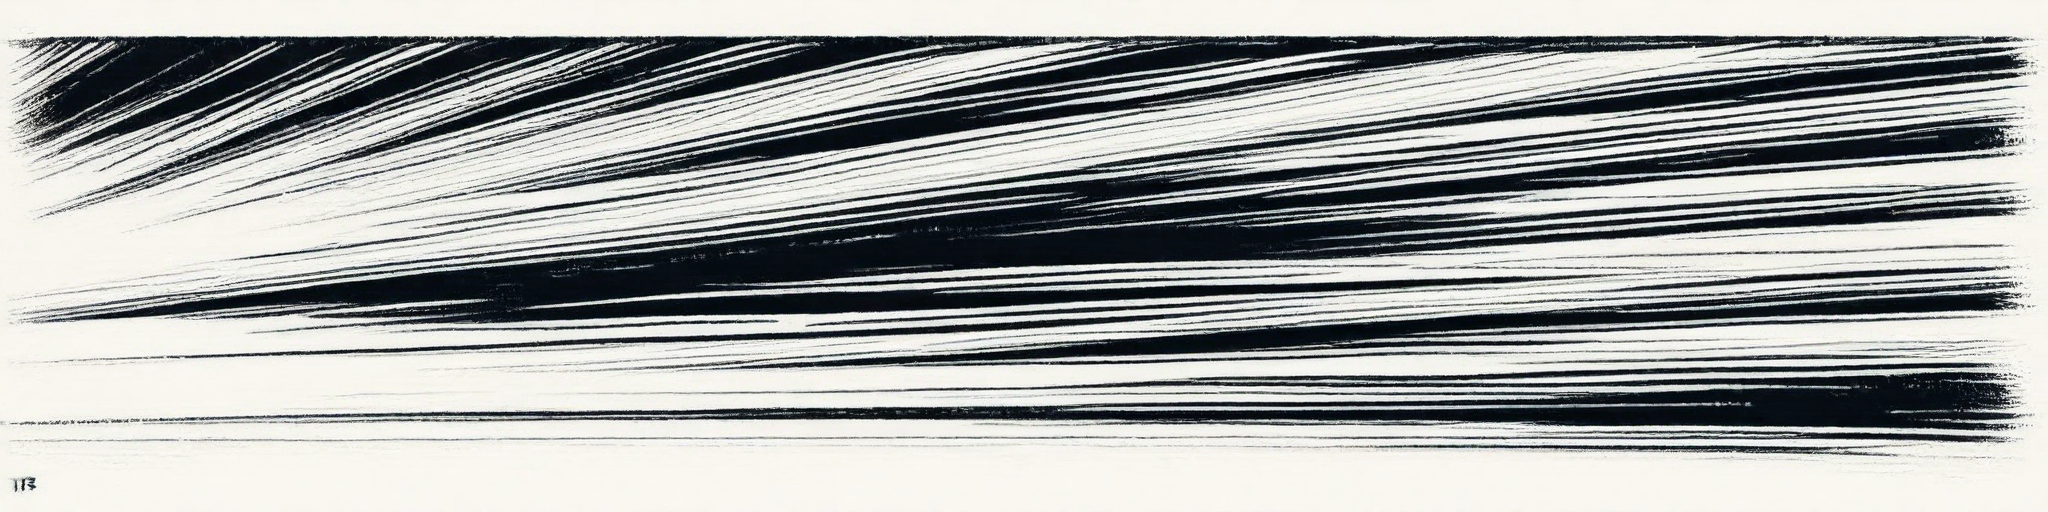
\includegraphics[width=\textwidth]{images/chapterImages/genesis_sketch_00119_.png}
\end{center}

Sarah woke at 3:17 AM with blueprints in her head.

Not metaphorical blueprints. Actual technical schematics. Satellite designs. Gravitational field generators. Orbital mechanics calculations. Knowledge she didn't have yesterday flooding in complete and perfect. She could see the entire defense grid. How it would deploy. How the satellites would coordinate. How the gravitational manipulation would work.

She reached for her laptop. Had to capture this. Had to record it before it faded.

It didn't fade. Just kept coming. More details. More systems. More understanding.

By 5 AM she'd filled forty pages of notes and the information was still flowing. Her hands were cramping. Eyes burning. Didn't matter. Had to get this down. Had to document everything.

By 7 AM she'd forgotten she'd meant to sleep. Food didn't occur to her. Shower didn't occur to her. Just the work. Just the relentless flood of understanding that needed to be captured, analyzed, implemented.

This was activation. This was what Marcus had been experiencing. This was the compulsion made real.

And it felt amazing.

That was the worst part. It felt right. Felt like coming home. Like finally understanding her purpose. Every discovery she'd ever made, every research breakthrough, every moment of scientific satisfaction—all of it was nothing compared to this. This was fulfillment. This was meaning. This was what she was designed to feel.

Like the first time she'd understood calculus, but more primal. Like the pull she'd felt at sixteen staring at equations until 4 AM, knowing her mother was worried but unable to stop. That same hunger, but infinite.

Her phone rang. She ignored it. Rang again. Again. Finally she picked up without checking who.

"What?"

"Sarah, it's Tom. Where are you? You missed the department meeting."

Tom. Her colleague. The meeting. She'd completely forgotten.

"I'm home. Working on something. Can't talk."

"Sarah, you're up for tenure review next month. You can't just skip—"

She hung up. Put the phone on silent. Turned back to her laptop.

The designs were more important than tenure. More important than her career. More important than everything.

By noon she'd contacted three aerospace engineers. Sent them partial designs. Waited for responses. They came back within hours—all confused, all intrigued, all asking the same question: How did you design this?

She didn't know how to answer. "Genetic activation" sounded insane. But it was the truth.

The responses kept coming. Engineers she'd sent designs to were sending modifications. Improvements. Additional systems. All of them spontaneous. All of them brilliant. All of them seemingly coming from nowhere.

The collective activation was happening. Thousands of people simultaneously receiving the same knowledge. The same capability. The same compulsion.

It was both terrifying and exhilarating.

Sarah's phone buzzed. Multiple messages. She glanced at them.

Tom: *Sarah, you need to call me. The dean wants to talk.*

Her ex: *You're late for Maya's birthday party. Where are you?*

She looked at the clock. 4:47 PM.

Maya's birthday.

Oh god. Maya's birthday.

She'd completely forgotten.

Sarah grabbed her keys. Ran to her car. Drove to Tom's house—her ex's house now. The house Maya lived in. The house Sarah visited twice a month if she remembered.

She arrived at 5:23. Cars in the driveway. Balloons on the mailbox. Party sounds from the backyard.

Sarah went around to the back gate. Found the celebration. Twenty kids. Parents. Cake. Maya in the center wearing a princess dress looking so happy.

Until she saw Sarah. Then the happiness drained. Replaced by something worse than anger. Resignation. Like Maya had learned not to expect anything and wasn't even disappointed anymore.

Tom saw her. His expression went cold.

"You're late."

"I'm sorry. I was working. I forgot—"

"You forgot your daughter's birthday."

The words hit like a physical blow. Sarah had forgotten Maya's birthday. Her eight-year-old daughter. The most important person in her life.

Except Maya wasn't the most important anymore. The work was more important. The compulsion made the work more important than everything.

For the work. For something she couldn't not do.

How many artists had said the same thing? How many musicians missed their children's recitals for one more session? How many writers chose the manuscript over the marriage? She'd judged them. Thought they were selfish. Thought they chose wrong.

Now she understood. They hadn't chosen at all.

"Maya, baby, I'm so sorry." Sarah approached. Tried to hug her daughter.

Maya stepped back. "You always say you're sorry."

"I know. I am. I brought your present—" Sarah hadn't brought the present. It was at home. Unwrapped. "—I'll give it to you later. Happy birthday, sweetie."

"I don't want a present."

"Maya—"

"I want you to remember. I want you to care. I want you to be my mom."

Sarah felt tears starting. "I am your mom. I do care. I just—"

"You were working. You're always working. You didn't come to my recital. You didn't come to my soccer game. You forgot my birthday. You don't love me anymore."

"That's not true. I love you so much."

"Then why don't you show it?"

Sarah didn't have an answer. Because the compulsion was stronger than love? Because she was genetically programmed to prioritize the work? Because her brain chemistry had been hijacked by activation sequences? None of that meant anything to an eight-year-old whose mother kept disappointing her.

Tom stepped in. "Maybe you should go, Sarah."

"I just got here—"

"And you're upsetting Maya. On her birthday. Which you forgot. Just... go. We'll talk later."

"I want to stay. I want to be here for—"

"Sarah." Tom's voice was quiet. Tired. "Look at yourself. When was the last time you slept? When was the last time you ate? You look like you're having a breakdown. Maya doesn't need to see you like this."

Sarah looked at her daughter. Maya was crying now. Quiet tears. Not dramatic. Just sad. Resigned to having a mother who didn't show up.

"I'm sorry," Sarah said again. Useless words. Empty words. "I'll make it up to you. I promise."

"You always promise," Maya said. "You never do."

Sarah left. Walked back to her car. Sat in the driver's seat with her hands shaking and tears running down her face.

She should stay. Should go back. Should fix this. Should prioritize her daughter over work.

But she could feel it. The compulsion. Pulling her attention back to the laptop. Back to the designs. Back to the work that provided relief from this emotional pain. The work that made sense. The work that was clear and purposeful and satisfying in ways parenting never was.

She started the car. Drove home. Opened her laptop. The designs were still there. Still demanding attention.

Sarah worked until 3 AM. Forgot about Maya's birthday. Forgot about her own failure. Forgot about everything except the defense grid.

The compulsion provided relief. Made the guilt manageable. Made the shame distant. Made everything except the work feel less real.

By morning, Maya's birthday was just a fact. A thing that had happened. Sarah felt bad about it. Would feel bad about it forever probably. But the badness was abstract. Intellectual. Not visceral anymore.

The compulsion had anesthetized her emotions. Made her effective. Made her functional. Made her into exactly the tool she was designed to be.

And she hated it.

And she couldn't stop it.

And she kept working anyway.

\scenebreak

Across the country, Marcus Chen hadn't come home in three days.

David found him in a rented warehouse in Oakland. Surrounded by equipment. Prototypes. Failed designs. Successful designs. Evidence of obsessive work at the expense of everything else.

"Marcus."

Marcus didn't look up. Was welding something. Sparks flying. Focus absolute.

"Marcus!"

He pulled off his welding mask. Looked at David like he was trying to remember who David was. Then recognition. "Hey. What time is it?"

"It's 4 AM. You didn't come home. You didn't call. I've been texting for two days. I thought you were dead."

"Sorry. I've been busy."

"Busy." David's voice was flat. "You've been busy. For three days. Without contacting me. Without telling me where you were. Without living in our apartment anymore apparently."

"I told you. The activation—"

"The activation. Right. The genetic compulsion. The thing you can't control." David moved closer. Saw the work space. The designs. The evidence of sophisticated engineering that Marcus shouldn't have been capable of. "What is all this?"

"Defense grid components. Gravitational manipulation systems. Orbital mechanics designs. I know how to build it, David. All of it. I can see exactly how it works."

"You're a mechanical engineer. You design industrial equipment."

"I was a mechanical engineer. Now I'm..." Marcus trailed off. Looked at his hands. "I don't know what I am now."

"You're my husband. Or you were. I'm not sure anymore."

Marcus set down his tools. Finally gave David his full attention. "I'm sorry. I know this is hard. I'm trying to—"

"You're not trying. You're completely consumed. You don't eat unless I remind you. You don't sleep unless you collapse. You don't talk unless I force you. You've disappeared into this work and I don't know how to get you back."

"I don't want to come back."

The words hung in the warehouse. Honest. Terrible. True.

David's expression cracked. "What?"

"I don't want to stop. I don't want to focus on anything else. This is the most important thing I've ever done. The most meaningful. The most right. And yes, it's programmed. Yes, it's activation. But it's still how I feel. The compulsion doesn't feel like slavery. It feels like purpose."

"More purpose than our relationship?"

"I don't know. Maybe. I'm sorry. But I can't lie to you. Can't pretend this isn't what I want even if wanting it is programmed."

David sat down on a crate. Looked at Marcus like seeing him for the first time. "Who are you?"

"I'm still Marcus."

"Are you? The Marcus I married wanted kids. Wanted to travel. Wanted to build furniture for our home and cook dinners and have conversations about books and movies. This person—" David gestured at the warehouse. "This person is a stranger. This person is obsessed. This person abandoned our life to build satellite components in a warehouse."

"The asteroid is real, David. If we don't build this defense grid, civilization ends. Billions of people die. Our future kids die. Everything dies. How do I choose our relationship over preventing that?"

"By being human. By recognizing that you're a person, not a tool. By exercising free will."

"What if I don't have free will? What if this compulsion is stronger than choice? What if I'm just code executing?"

"Then you're not responsible for abandoning me. But you're also not a person. You're just a program. And I can't be married to a program."

Marcus wanted to argue. Wanted to prove he was still himself. Still capable of love. Still choosing David despite the compulsion.

But he couldn't. The compulsion was always there. Always pulling. The moment this conversation ended, he'd go back to work. He knew it. David knew it. The relationship was already over. Just neither of them had acknowledged it yet.

"I'm sorry," Marcus said. "I love you. That's real. But I can't be what you need anymore."

"Can't or won't?"

"I don't know the difference."

David stood. "I'm leaving. Moving back to my sister's place in Portland. I'll get the rest of my stuff next week. I'll file the divorce papers. You... do whatever you're programmed to do."

"David—"

"Don't. Don't apologize again. Don't tell me you love me while choosing the work. Don't insult me by pretending you're trying."

He left. Marcus watched him go. Felt something break inside. Grief. Loss. The end of everything personal and private and beautiful they'd built together.

And underneath the grief: relief. Relief that he didn't have to balance anymore. Didn't have to pretend the relationship was as important as the work. Could fully commit to the compulsion without guilt.

The relief made him hate himself. But he turned back to his welding anyway.

The work demanded attention. The work provided satisfaction. The work was what he was designed to do.

David was right. Marcus wasn't a person anymore. Was just code executing. Just purpose. Just tool.

And he couldn't bring himself to care enough to fight it.

The compulsion had won.

\scenebreak

Around the world, the pattern repeated. Activated individuals abandoning relationships. Quitting jobs. Leaving lives. All driven by the same irresistible need to build.

Social media filled with confused posts. People describing the same symptoms. The intrusive knowledge. The compulsion. The inability to focus on anything except the work. Support groups formed. Forums emerged. People trying to understand what was happening to them.

And slowly, the realization spread: this was real. This was widespread. This was activation.

The secret couldn't hold. Too many people experiencing the same thing. Too many unexplainable capabilities emerging simultaneously. Too many brilliant designs coming from people who shouldn't have the knowledge to create them.

The media started reporting. At first skeptically. Then with growing concern. Then with something approaching panic. Thousands of engineers and physicists were experiencing simultaneous compulsion to build the same defense system. All claiming genetic programming. All showing evidence of capabilities beyond their training.

Either mass delusion or something unprecedented happening to human consciousness.

Governments got involved. Researchers like Sarah were contacted. Asked to explain. Asked to verify. Asked to help make sense of what was clearly happening but shouldn't be possible.

Sarah explained. Showed the genetic data. Demonstrated the correlation. Proved that activation sequences were expressing exactly on schedule.

The evidence was undeniable. Humanity was programmed. The activation was real. The compulsion was biological. And thousands of people were being transformed into something they hadn't chosen to become.

The philosophical implications could wait. The immediate concern was: what were all these activated people building? And should anyone try to stop them?

Sarah's answer was simple: They're building planetary defense. Against a real asteroid. On a real timeline. Stopping them means accepting extinction. Letting them continue means surrendering autonomy. There's no good option. Just necessary action.

The world chose necessity. Governments provided resources. Facilities. Coordination. The activated individuals self-organized. Built networks. Shared designs. Worked with collective purpose toward the same goal.

A global defense grid emerging from coordinated compulsion. Humanity working together not by choice but by programming. Building their salvation through the loss of free will.

And Sarah Chen, having missed her daughter's birthday to document activation, watched it all unfold with guilt and fascination and the growing certainty that she'd lost Maya forever.

The work continued.

The compulsion intensified.

The relationships fractured.

And the program executed regardless of cost.

Because that's what programs do. They execute. Regardless. Always. Without mercy.

The equation balanced.

The code ran.

The defense built itself.

And the people who were building it slowly stopped being people.

Became tools instead.

Conscious tools. Aware tools. Tools that suffered.

But tools nonetheless.

The activation was complete.

The transformation irreversible.

The purpose absolute.

And nothing—not love, not guilt, not the desperate need to be human—could stop it.


\chapter{The Compulsion}
\label{ch:23}



\begin{center}

\includegraphics[width=\textwidth]{images/chapterImages/genesis_sketch_00120_.png}
\end{center}

Six months after full activation, Sarah weighed 118 pounds. She'd been 142 before. The weight loss happened gradually then suddenly. Food was interruption. Sleep was interruption. Anything that wasn't work was noise to be minimized.

She looked at herself in the bathroom mirror—rare moment of self-awareness between work sessions—and barely recognized the person staring back. Hollow eyes. Sharp cheekbones. Hair she'd been cutting herself because salons took time. She looked like the addicts she'd seen in documentaries. That comparison had stopped bothering her months ago.

Her apartment was a workspace now. Tables covered in laptops and printouts. Whiteboards on every wall. Sleeping bag in the corner because the bedroom was too far from the work. Shower once every three days. Food delivered, eaten while reviewing data, barely tasted.

This was what activation looked like. This was the cost of purpose.

Her phone sat on the counter. Seventeen missed calls from Tom. Four from Maya's school. Sarah picked it up. Listened to the voicemail from three days ago.

*Sarah, it's Tom. Maya's asking about you again. She wants to know if you're coming to her school play. I told her probably not but she's still hoping. Can you just... I don't know. Send her a message? Let her know you're alive? She's worried. I'm worried. Everyone's worried.*

Sarah put the phone down. Opened her laptop. Started composing an email to Maya.

*Dear Maya,*

*I'm sorry I can't make your play. I'm working on something important. Something that*

She stopped. Deleted it. Started again.

*Maya,*

*I love you. I'm sorry I'm not*

Deleted. Tried once more.

*Sweetie,*

*I*

She closed the laptop. Couldn't find words that weren't lies. "I love you" was true. "I'm sorry" was true. But "I'll try to be there" was false. She wouldn't try. Couldn't try. The compulsion wouldn't allow prioritization of anything except the work.

Sarah opened her laptop again. Not to write to Maya. To review the latest defense grid calculations. The email to her daughter forgotten within seconds.

This was how it worked. The intention to connect. The attempt to maintain relationships. Then the work pulling attention back. Every time. Always. The compulsion was stronger than will. Stronger than love. Stronger than everything.

\scenebreak

Marcus had moved entirely into the warehouse. It wasn't home—home required personal touches, comfort, life. This was just workspace. Place to build and sleep for four hours and build again.

The divorce papers had arrived three weeks ago. He'd signed them without reading. Sent them back. David was gone. That relationship was over. Acknowledging it legally was just paperwork.

He felt bad about that. In the abstract. The way you feel bad about news stories. Distant tragedy. Not visceral pain. The compulsion had numbed him. Made everything except the work feel less real.

Sometimes at night—when exhaustion forced a break—Marcus would remember what he'd lost. David's laugh. The way he'd correct Marcus's grammar. The smell of his soap. The future they'd planned. Kids. Growing old together. All of it gone.

And Marcus would feel grief. Real, deep grief. For maybe five minutes. Then the compulsion would surge. The designs would demand attention. Relief would come from turning back to the work.

The grief didn't stop the compulsion. The compulsion stopped the grief. Made it manageable. Made it survivable. Made it irrelevant.

His warehouse had become a hub. Twenty other activated individuals working there. All driven by the same compulsion. All building components of the defense grid. All sacrificing everything for purpose they didn't choose.

They barely talked. Didn't need to. Everyone knew what needed to be done. Everyone worked their piece. The coordination was automatic. Organic. Like watching ants build a colony—individual action serving collective function without explicit communication.

Sometimes visitors came. Journalists. Researchers. People trying to understand the phenomenon. Marcus would answer questions while his hands kept working. Multi-tasking. Never stopping. Never fully present for anything except the work.

"How does it feel?" they'd ask. "The compulsion. Can you describe it?"

"Like remembering something I'd forgotten," Marcus would say. "Like the knowledge was always there, just waiting. Like coming home."

"Is it pleasant?"

"It's fulfilling. Whether fulfillment is pleasant or just absence of discomfort, I don't know. But when I'm working, everything makes sense. When I stop, everything falls apart. So I don't stop."

"Do you want to stop?"

"No. That's the problem. I don't want to stop. Which means maybe it's not compulsion. Maybe it's just who I am now."

"Do you miss your old life?"

"Yes. But missing it doesn't make me want it back. That's the distinction. I can recognize what I've lost and still prefer the work. Can grieve the relationship while being relieved it's over. Can be both things simultaneously."

"Does that make sense?"

"No. But it's true anyway."

The journalists would leave. Marcus would keep working. The designs demanding attention. The purpose consuming everything.

\scenebreak

Globally, the pattern was consistent. Activated individuals displaying the same behaviors:

Sleep deprivation. Average 4.2 hours per night. Some going days without sleep before collapsing.

Weight changes. Most losing weight. Some gaining from stress eating. All showing signs of physiological stress.

Social isolation. Relationships ending. Friendships dissolving. Families giving up trying to stay connected.

Workplace abandonment. 73\% of activated individuals had quit or been fired from jobs. The work paid nothing. Purpose wasn't profitable. But the compulsion didn't care about economics.

Living situations declining. Moving into workspaces. Neglecting hygiene. Eating whatever was convenient. Life becoming purely functional. Nothing wasted on comfort.

And through it all: productivity. Unprecedented productivity. Designs emerging at rates that shouldn't be possible. Prototypes being built and tested. Systems being integrated. The defense grid advancing from concept to reality in months instead of decades.

It was working. The activation was achieving its purpose. Humanity was building the defense system exactly on schedule.

The cost was just humanity itself. The activated were becoming tools. Conscious tools. Suffering tools. But tools nonetheless.

\scenebreak

Sarah attended exactly one research conference during those six months. James insisted. Said she needed to present findings. Needed to maintain academic credibility.

She went. Gave her presentation. Answered questions with minimal engagement. Left as soon as she could.

At the hotel bar afterward, Katherine found her.

"You look terrible," Katherine said. No preamble. No social niceties. Blunt assessment.

"You too."

It was true. Katherine had aged years in months. Hair showing gray. Skin showing stress. The same hollow intensity everyone activated shared.

"Sleeping?" Katherine asked.

"No."

"Eating?"

"When I remember."

"Same."

They sat in silence. Two activated individuals recognizing shared destruction.

"I miss feeling human," Katherine said quietly. "I miss wanting things that aren't work. I miss having desires beyond the compulsion. I miss being Katherine instead of just being purpose."

"Do you remember the Fields Medal?" Sarah asked. "Your pride in winning it?"

"Barely. It feels like someone else's memory. Like I'm remembering a character from a book."

"I feel the same about Maya. I remember being her mother. Remember loving her. But it's distant. Like watching old home movies. The person in those memories isn't me anymore."

"What are we?"

"Programs executing."

"Are we suffering?"

"I don't know. I think I should be suffering. Should be devastated. But the compulsion anesthetizes it. Makes the loss manageable. Makes the work more important than the pain."

Katherine finished her drink. "That might be the cruelest part. Not that we're programmed. That the programming makes us okay with being programmed. Makes us prefer it. Makes us grateful for purpose even as purpose destroys us."

"Are you grateful?"

"I don't know. I'm fulfilling my function. Is that the same as grateful? Or is that just another way the code executes?"

No answer. Just the bar noise. Normal people living normal lives. Unactivated. Uncompelled. Free in ways Sarah and Katherine would never be again.

"I should go," Sarah said. "Need to review data."

"At 11 PM?"

"The work doesn't care what time it is."

"No. It doesn't."

They left separately. Both returning to hotel rooms to work. Both driven by compulsion stronger than fatigue. Both aware they were losing themselves and unable to care enough to stop.

The program executed. The people faded. The work continued.

\scenebreak

In Portland, David was trying to move on. Dating someone new. Teacher at his school. Nice. Uncomplicated. Not obsessed with anything. Not compelled by genetics.

But at night, David would think about Marcus. Wonder if he was okay. Wonder if he was eating. Wonder if he even remembered what they'd been to each other.

He'd check Marcus's social media sometimes. Rare posts. Always about the work. Always showing the warehouse. Always evidence of ongoing obsession.

David had been angry at first. Then hurt. Then resigned. Now he just felt sad. Sad for Marcus. Sad for what they'd lost. Sad for the future they'd never have.

And guilty. Guilty for leaving. Even though Marcus had chosen the work. Even though the relationship was unsustainable. David still felt like he'd abandoned someone who was sick. Because the compulsion was sickness. Genetic sickness. Sickness that looked like purpose.

His new boyfriend asked about it once. "You think about him? Your ex?"

"Sometimes."

"You still love him?"

"I love who he was. I don't know if that person exists anymore."

"Would you take him back? If he stopped the work?"

"He can't stop the work. That's the point. He's genetically compelled. The choice isn't there."

"Then it's not his fault."

"Doesn't make it hurt less."

They didn't talk about it again. David moved forward. Built new life. But in quiet moments, he grieved. For Marcus. For himself. For the relationship that died to genetic programming.

\scenebreak

By six months, the activated were visibly different. You could spot them. The intensity. The focus. The hollow look of people consuming themselves for purpose.

Support networks formed. Family members of activated individuals trying to understand. Trying to cope. Trying to grieve people who were still alive but no longer fully present.

Therapists specialized in it. "Activation grief counseling." How to accept that your loved one is choosing work. How to understand it's not really choice. How to let go of someone who hasn't died but is no longer reachable.

Children of activated parents showing signs of trauma. Abandonment issues. Anger. Confusion. Schools developing protocols. Social services investigating. The personal cost of saving civilization becoming visible.

Maya Chen—now Maya Patterson, using her stepfather's name—drew a picture in therapy. Her family. Tom and his new partner. Her baby brother. And off to the side: a stick figure labeled "Mom" with a computer. Far away. Separate. Not part of the family.

The therapist asked: "How do you feel about your mom?"

"I don't know."

"Are you angry?"

"Sometimes. Mostly I'm just sad. And tired of being sad."

"Do you love her?"

"I think so. But I don't know her anymore. She's someone else now. Someone who doesn't have time for me."

"Would you want her back? If she could stop working?"

Long pause. Then: "No. Not anymore. I don't want someone who only stays because they have to. I want someone who wants to be there. And she doesn't want to be there. So I don't want her."

Eight years old. Already learning that some losses can't be fixed. Some relationships can't be saved. Some mothers choose work over daughters and there's nothing the daughters can do.

The cost of the defense grid measured in broken children. In ended relationships. In people who stopped being people to become functions.

And Sarah Chen, reviewing genetic data at 2 AM and forgetting she had a daughter, was both perpetrator and victim of that cost.

The compulsion didn't care about fairness. Didn't care about suffering. Didn't care about anything except completion.

The work continued. The people hollowed. The purpose executed.

And the only comfort was knowing it was working. The defense grid was forming. The capability was real. The asteroid would be stopped.

Civilization would survive. At the cost of the civilization of those who saved it.

Balance. Equation. Price.

The mathematics was complete. The code ran perfectly. The program achieved its purpose.

And the activated individuals, having fulfilled their function, had nothing left except the ongoing compulsion to keep building, keep working, keep sacrificing everything for purpose that felt like fulfillment and looked like destruction.

The line between the two invisible. Irrelevant. Gone.

Just work. Just purpose. Just compulsion.

Forever.

Or until the grid was complete.

Whichever came first.

They all hoped for completion. Hoped the compulsion would release them. Hoped they could return to being human afterward.

But none of them believed it. The compulsion was permanent. The transformation irreversible. The loss absolute.

They were tools now. Would be tools forever. Conscious, aware, suffering tools. But tools nonetheless.

The equation balanced. The program executed. The cost paid.

And humanity built its salvation through the destruction of those who built it.

Perfect efficiency. Perfect purpose. Perfect horror.

The code continued. The work continued. The people faded.

And the only thing that mattered was the work.

Always the work. Only the work. Forever the work.


\chapter{The Choice}
\label{ch:24}



\begin{center}
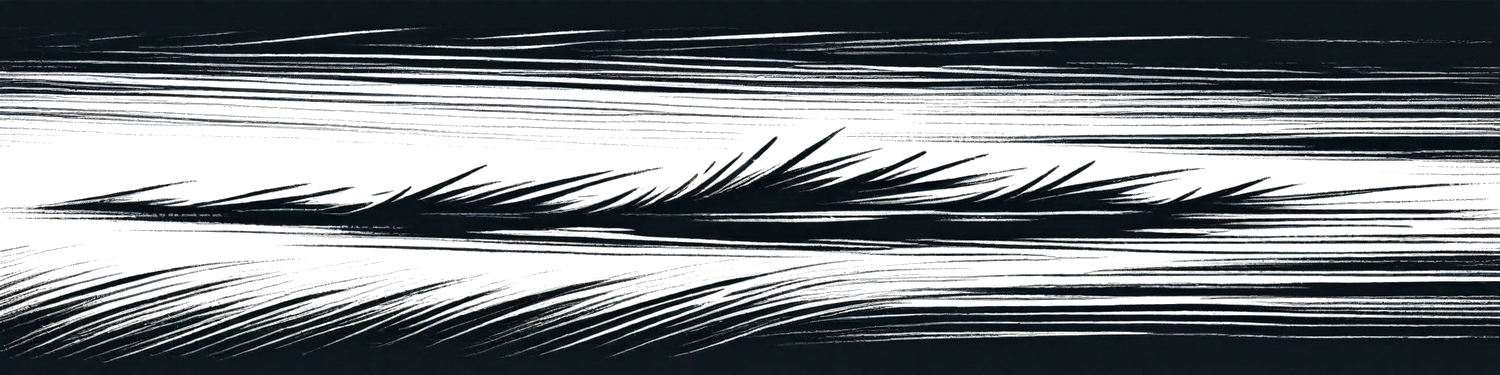
\includegraphics[width=\textwidth]{images/chapterImages/genesis_sketch_00121_.png}
\end{center}

The emergency meeting convened at 3 AM. Not because of urgency—everything was urgent now—but because it was the only time enough key researchers could be present simultaneously. The activated worked on their own schedules. Sleep happened when exhaustion forced it.

Sarah arrived at the conference room to find twelve people already there. Katherine. James. Marcus sitting in the corner, looking worse than when she'd seen him six months ago. Several others she recognized from papers. All activated. All hollow. All driven.

"Thank you for coming," James said. He looked the most normal of them—still showering regularly, still dressing professionally. But the exhaustion showed in his eyes. In everyone's eyes. "We have a decision to make. A significant one."

He pulled up data on the main screen. Astronomical observations. Trajectory calculations. Impact probabilities.

"This is 2027 RL₃," James said. "Asteroid. 1.7 kilometers diameter. Currently in outer solar system. We've been tracking it for eighteen months. Initial projections showed it would pass Earth at safe distance."

He clicked to the next slide. New calculations. Different trajectory.

"Three days ago, it had a close encounter with Jupiter. Gravitational perturbation. The trajectory changed."

Another click. Impact map. Probability calculations.

"New impact probability: 94.3\%. Time to impact: 38 years, 7 months."

Silence in the room. Everyone processing. Everyone calculating. Everyone arriving at the same conclusion simultaneously.

"Thirty-eight years," someone muttered. "Our children's problem. Easier to ignore than tomorrow's problem."

"Exactly," James said. "Which is why this one will get solved. The urgency is abstract enough to think about, immediate enough to act on. Unlike—" He stopped himself.

Unlike other things, Sarah thought. Unlike the warming everyone knows about but no one with power will admit is this urgent. At least this time, the activation makes action inevitable.

"The defense grid isn't designed for this timeline," someone said. Martinez, maybe. Physicist. Heavily activated. "We calculated for 60-year minimum. This is twenty years shorter."

"Can we accelerate?" Katherine asked.

"Unknown. Probably. But it would require significantly more resources. More activated individuals. More sacrifice." James looked around the room. "Which brings us to the decision. Do we tell people?"

"Tell people what?" Sarah asked. "That there's an asteroid? That we're building defense capability? That we're genetically compelled?"

"All of it. The public knows something is happening. Thousands of people worldwide suddenly obsessed with building the same thing. Families being destroyed. Resources being diverted. They're asking questions. We've been deflecting. But if we need to accelerate—if we need public support, government funding, global coordination—we need to tell the truth."

"The whole truth?" Marcus asked quietly. "That humanity is programmed? That our evolution is engineered? That free will might be illusion?"

"Yes."

The room erupted. Multiple people talking simultaneously. Arguments overlapping. The core debate immediate:

Some argued for disclosure. The asteroid was real. The threat was existential. People deserved to know. Deserved to understand why the activated were sacrificing everything. Deserved to choose whether to support the work.

Others argued against. The revelation would cause panic. Social collapse. Existential crisis on global scale. Better to build quietly. Finish the grid. Save humanity. Tell them afterward.

Sarah listened to both sides. Understood both positions. Couldn't choose between them.

"What does the genetic data suggest?" Katherine asked. Turning to Sarah. "Did Aurelia intend for us to know? Is there disclosure built into the program?"

Sarah thought about this. Reviewed what she knew. The activation sequences. The capability thresholds. The timeline programmed into mammalian DNA 65 million years ago.

"There's no specific disclosure sequence," she said. "But the activation was always going to be obvious. Thousands of people worldwide simultaneously developing the same capability, building the same thing? That was going to raise questions. Aurelia must have known we'd figure it out."

"So disclosure was planned?"

"Or inevitable. Or irrelevant. I don't know what Aurelia thought about human psychology. They were reptilian intelligence. Maybe they didn't consider whether we'd want to know. Maybe they just built the capability and assumed we'd use it."

"We are using it," Marcus said. "Everyone in this room is using it. The question isn't whether the capability works. It's whether revealing the source helps or hurts."

"And whether we have the right to hide it," James added. "Whether choosing for humanity is better or worse than letting humanity choose for itself."

"Can humanity choose?" Katherine asked. The core question. The question beneath everything. "If we're programmed, is collective choice possible? Or is disclosure versus secrecy just different execution paths of the same code?"

No one had an answer.

Sarah looked around the room. At the activated individuals. At the people whose lives had been consumed by genetic compulsion. At the researchers who'd lost everything to build something they couldn't choose not to build.

"I want to tell people," she said quietly. "Not because I know it's right. But because hiding this feels like being ashamed of what we are. And I'm not ashamed. I'm compelled, I'm suffering, I'm losing everything that matters—but I'm not ashamed."

"Why not?" someone asked.

"Because Aurelia did this for us. Because 65 million years ago, beings who knew they were going to die chose to program our capability because they loved this planet enough to protect it even after they were gone. That's not something to hide. That's beautiful."

Marcus spoke from the corner. "Every artist thinks that. That the compulsion is gift, not curse. That sacrificing your life for your work is noble." He looked at his hands. "David thought I was choosing the work. Thought I could stop. I thought—" His voice cracked. "I thought I was choosing too. That the drive was mine. That I was doing something that mattered."

"It does matter," Sarah said.

"Does it? Or does it just feel like it matters because we're programmed to feel that way? Every creator who destroys themselves for their art thinks it's meaningful. But what if it's just—" He gestured helplessly. "—just code. Running."

Silence filled the room.

"It's also horrifying," Martinez said quietly. "It means we're tools. Biological machines executing someone else's program."

"We're both," Sarah said. "Beautiful and horrifying. Programmed and capable. Tools with consciousness. The contradiction doesn't resolve. But hiding from it doesn't make it less true."

Katherine leaned forward. "If we disclose, the social cost will be enormous. Religions will fracture. Philosophies will collapse. People will spiral into nihilism. The suicide rate will spike. The activated are already suffering—disclosure will make everyone suffer."

"Are you arguing for secrecy?"

"I'm arguing that we should count the cost before we decide." Katherine's voice was sharp. Tired. "I've lost everything. My career, my relationships, my sense of self. I've accepted that cost because the work matters. But I accepted it myself. I don't want to impose existential crisis on people who aren't activated. Who don't need to know. Who might be happier not knowing."

"Is ignorance kindness or condescension?" James asked.

"I don't know. But I know suffering. And I know disclosure will cause suffering. Is that worth it? For what? Transparency? Honesty? Those are values we made up. Maybe values that were programmed. Who's to say honesty is more important than peace?"

Sarah thought about Maya. About telling her daughter that mommy couldn't come to the school play because mommy was genetically compelled to save the world. About explaining that free will was questionable and meaning was ambiguous and love might be chemistry.

Maya was eight years old. She didn't need that. Didn't deserve that burden.

But she also deserved truth. Deserved to understand. Deserved to know that her mother wasn't choosing work over her—or was choosing but couldn't not choose—or some horrible tangled mess of programming and intention that no one could untangle.

Which was kinder? The truth or the lie?

"We should vote," James said. "Everyone activated has stake in this. We're the ones who'll face the consequences either way. Show of hands. Who supports disclosure?"

Sarah raised her hand. Slowly. Still uncertain but committed.

Marcus raised his. Katherine didn't. Martinez did. Four others raised theirs. Five kept hands down.

Nine to eight. Close. Too close.

"Not enough consensus," James said. "We need more time. More discussion. We—"

"We don't have time," Sarah interrupted. "The asteroid is coming in 38 years. We need to accelerate. That requires public support. That requires disclosure. Or we build in secret, probably fail, and humanity dies without understanding why."

"Or we succeed without disclosure and humanity survives without unnecessary suffering."

"Is it unnecessary? To know what you are? To understand why you're capable of greatness? To see the inheritance passed down from extinct beings who loved us before we existed?"

"Is that what you'll tell people?" Katherine asked. "That dinosaurs loved us? You think that'll be comforting? You think people will hear 'you're programmed by extinct reptiles' and feel loved?"

"I think people deserve the truth. Even if the truth is uncomfortable."

"Even if the truth drives them to despair?"

"Even then."

They stared at each other. Two brilliant women. Two activated individuals. Two people who'd lost everything to genetic compulsion. Disagreeing about whether loss should be shared or contained.

"Let's table this," James said. "We'll reconvene in a week. Everyone think about it. Run calculations. Consider implications. We decide together or we don't decide at all."

The meeting ended. People dispersed. Returning to work. Always returning to work.

Sarah found Marcus in the hallway. Leaning against the wall. Looking exhausted.

"You voted for disclosure," she said.

"Yeah."

"Why?"

"Because David asked me once if I needed him or wanted him. And I couldn't answer. Couldn't tell the difference. And he said that was the point—that if I could separate need from want, it probably wasn't real." Marcus looked at her. Eyes hollowed. Grief visible. "I think about that conversation a lot. I think about whether anything I feel is real or just programming. And I think... I think the only way to know is to look directly at it. To see the code. To understand what we are. Hiding from it doesn't make it less true. Just makes us less aware."

"What if awareness is worse than ignorance?"

"It probably is. But it's honest. And I'd rather be honestly miserable than comfortably deluded."

"That's bleak."

"That's where I am."

Sarah thought about the compulsion. About the work consuming her. About Maya growing up without a mother. About Aurelia standing over The Companion's body before returning to work.

"If we disclose," she said, "people will hate us. Will blame us for revealing it. Will wish we'd kept the secret."

"Probably. But we're already losing everything. What's one more loss?"

"Our legacy? Our place in history? We could be remembered as saviors. Instead we'll be remembered as the people who proved humanity was programmed."

Marcus laughed. Bitter. Broken. "We're not saviors. We're just the ones who happened to activate at the right time. The program ran. We executed. Claiming credit for that is like claiming credit for breathing."

"So we should tell people we're meaningless?"

"We should tell people the truth and let them decide what it means."

Sarah didn't respond. Just stood in the hallway with Marcus. Two people who'd never be close but understood each other in ways no one else could. Both activated. Both compelled. Both choosing disclosure without knowing if choice was real.

"I'm going to call Maya," Sarah said suddenly. "Going to try to explain. Going to tell her why I haven't been there. See if she can understand."

"Will she?"

"No. She's eight. She just wants her mom. But maybe when she's older. Maybe when she's activated herself—if she has the markers—maybe she'll remember this conversation and understand."

"Or maybe she'll remember that you tried. That you reached out. That you did something that wasn't work."

"Maybe."

Sarah pulled out her phone. Looked at it. Forty-seven missed calls. Sixty-three unread messages. All from people she was ignoring. People she'd stopped being present for.

She dialed Tom's number. It rang four times before he answered.

"Sarah?"

"Is Maya awake?"

"It's 4 AM."

"I know. I just... I need to talk to her. I need to explain. Can you wake her up? Please?"

Silence on the other end. Then: "Sarah, I don't think—"

"Tom, please. I know I don't deserve it. I know I've been absent. But I need to try. Just this once. Please."

More silence. Then: "Hold on."

She heard movement. Heard Tom talking quietly. Heard Maya's sleepy voice asking who was calling.

Then: "Mom?"

"Hi sweetie."

"Why are you calling? Is something wrong?"

"No. Nothing's wrong. I just... I wanted to talk to you. Wanted to explain why I haven't been around. Wanted you to know it's not because I don't love you."

"I know you love me."

"Do you?"

"Dad says you're sick. Says you can't help it. Says you're working on something important and you can't stop."

"That's... that's close to true. I'm not sick exactly. But I can't stop. You're right about that."

"Why not?"

How did you explain genetic compulsion to an eight-year-old? How did you describe feeling driven by forces you couldn't control? How did you make it sound like anything other than choosing work over daughter?

"Do you remember when we talked about instincts?" Sarah asked. "How birds know to fly south without being taught? How spiders know to spin webs?"

"Yeah."

"I have something like that. An instinct. But for humans. For building things. For solving problems. And right now, that instinct is very, very strong. So strong I can't think about anything else. So strong I forget to eat and sleep and... and call my daughter."

"That sounds scary."

"It is scary. For me and for you. And I'm sorry you have to deal with it. Sorry I can't be the mom you need right now."

"When will you be done? When can you be normal again?"

Sarah felt something break in her chest. The same thing that broke when she discovered the genetic code. When she realized her capability was programmed. When she understood that Aurelia had built this into her 65 million years ago.

"I don't know, sweetie. I hope soon. But I don't know."

"Okay."

"Okay?"

"I miss you. But Dad says you're doing important work. Says you're helping people. So it's okay. I just wish you could help people and also be my mom."

"Me too. I wish that so much."

"I made a drawing of you. Want me to send it?"

"I'd love that."

"Okay. I'm gonna go back to sleep now. Is that okay?"

"That's okay. Thank you for talking to me."

"Love you, Mom."

"I love you too. So much."

The call ended. Sarah stood in the hallway. Phone in hand. That broken thing in her chest expanding. Filling her. Overwhelming everything.

She cried. Actually cried. For the first time in months. Standing in the hallway at 4 AM. Crying for her daughter. For herself. For Aurelia who'd had young and left them to encode the future. For every being who'd ever chosen purpose over presence.

Marcus stood nearby. Watching. Not intervening. Just present.

After a few minutes, Sarah composed herself. Wiped her face. Put the phone away.

"You okay?" Marcus asked.

"No. But I'm going to keep going anyway."

"Yeah."

"We should disclose. Should tell people. Should give Maya and every other child of activated individuals the truth. They deserve to know why their parents can't stop working. Deserve to understand that it's not choice and also is choice and the distinction doesn't matter because the compulsion is real either way."

"Will that make it easier for them?"

"No. But it'll make it honest."

Marcus nodded. "I'll support whatever you decide. At the vote. If you want disclosure, I'll argue for it."

"Why? Why support me specifically?"

"Because you're still crying for your daughter. Because the compulsion hasn't erased that. Because if we're going to tell people we're programmed, I want the person delivering the message to be someone who still visibly loves something more than the work."

"I don't love her more than the work. If I did, I'd be there."

"You called her at 4 AM. That's something. That's more than most activated people are doing. That's proof that programming isn't absolute. That some part of you still chooses. Still fights. Still tries."

"Is trying enough?"

"It has to be. It's all we have."

They stood in the hallway. The building quiet. The work continuing somewhere below. The compulsion waiting to pull them back.

But for this moment—this small moment of grief and recognition and shared understanding—they were people. Not tools. Not programs. Just people trying to navigate impossible choices with insufficient information and questionable autonomy.

"I should get back to work," Sarah said.

"Yeah. Me too."

They separated. Returning to their stations. Returning to the compulsion. Returning to the work that would consume them until the grid was complete or they died trying.

But something had changed. Some decision made. Some clarity achieved.

They would tell the truth. Would disclose the programming. Would show humanity what it was.

And whatever came after—panic, despair, acceptance, rage—would be honest. Would be real. Would be chosen as much as anything could be chosen by beings who might be executing code.

The asteroid was coming. 38 years and counting. Humanity needed to build its defense. Needed to use the capability Aurelia had encoded.

And humanity deserved to know what that capability was. Where it came from. What it cost.

Sarah returned to her apartment. Opened her laptop. Started drafting the disclosure statement.

It would take weeks to finish. Months to refine. Would require approval from the research network. Would need to be translated into dozens of languages. Would need to be released carefully to minimize panic.

But it would be released. The truth would be told. The programming would be revealed.

And whatever happened next—whatever suffering or understanding or horror or acceptance emerged—would be humanity's to experience.

Fully informed. Fully aware. Fully human even if humanity was programmed.

The compulsion hummed. The work called. Sarah answered.

But she kept Maya's picture when it came. Pinned it above her desk. Reminder that purpose wasn't everything. That love—whatever love was—persisted even when compulsion dominated.

The code executed. The program ran. But the person inside the program still chose to cry. Still chose to call. Still chose to remember.

And maybe that was enough.

Maybe that was the only freedom anyone ever had.

The choice to care even when caring hurt. The choice to try even when trying wasn't enough. The choice to love even when love competed with compulsion.

Maybe that was what Aurelia had given them. Not just capability. But the capacity to choose despite the code. To act despite the programming. To love despite the compulsion.

Or maybe that was just another subroutine. Another layer of code. Another way the program executed.

Sarah didn't know. Would never know. Couldn't know.

But she chose to believe it mattered. Chose to act like it was real. Chose to disclose and cry and love and work and suffer.

And maybe the choosing—even if predetermined—was enough.

The mathematics was complete. The decision was made. The truth would be told.

And humanity would face what it was. Together. Honestly. Completely.

Whatever came next was inevitable. Was necessary. Was real.

The program continued. The work continued. The disclosure prepared.

And Sarah Chen, mother and scientist and programmed being, chose to keep going.

Because the work mattered. Because Maya mattered. Because truth mattered.

Because 38 years wasn't much time. And humanity needed to know what it was building. Why it was building. What inheritance it was using.

The asteroid was coming. The defense would be built. The truth would be told.

And whatever happened after—whatever collapse or growth or synthesis or catastrophe—would be humanity's to experience.

Fully human. Fully programmed. Fully alive.

All of it simultaneously. All of it real. All of it theirs.

The choice was made. The path was set. The disclosure would proceed.

And Sarah Chen, having chosen as much as anyone could choose, returned to the work that would save the world and destroy her life and prove that both things could be true simultaneously.

The program executed. The person persisted. The love remained.

And that was enough. Had to be enough. Was all anyone ever had.

The mathematics was complete. The decision was made.

The truth would be told.


\chapter{The Broadcast}
\label{ch:25}


The video was simple. No special effects. No dramatic music. Just Sarah Chen sitting in a plain room with a camera and the weight of 65 million years of genetic programming on her shoulders.

She'd recorded it seventeen times. Each version different. Each attempt trying to find the right tone. The right words. The right way to tell humanity that everything they thought about themselves was wrong.

This was take eighteen. The final version. The one they'd decided to release.

Sarah looked at the camera. Took a breath. Began.

"My name is Dr. Sarah Chen. I'm a geneticist. For the past three years, I've been studying patterns in human DNA that don't make sense according to conventional evolutionary theory. Today I'm going to tell you what I found. And I need you to understand: this is not speculation. This is not theory. This is verified, peer-reviewed fact supported by evidence from multiple independent research teams across the globe."

She paused. Let that settle. Let people understand this was serious.

"65 million years ago, an intelligent species existed on Earth. Not humans. Not mammals. A species of reptilian intelligence that we've come to call 'The Architects.' They were brilliant. Capable of complex calculation, long-term planning, and—critically—genetic engineering at a level we're only beginning to understand."

Another pause. She could feel the weight of what came next. The revelation that would break everything.

"The Architects detected an incoming asteroid. They calculated impact probability at near 100\%. They knew they were going to die. They couldn't save themselves. But they could save the planet. They could encode planetary defense capability into small mammals that would survive the extinction event. They could program evolution. Program capability. Program *us*."

Sarah pulled up images. DNA sequences. Activation markers. Mathematical proofs.

"This is what they did. They modified mammalian DNA to include specific capability thresholds. Tool use. Fire. Agriculture. Writing. Mathematics. Astronomy. And finally—planetary defense. Each capability encoded to activate when environmental conditions triggered it. Each threshold timed to ensure maximum survival probability."

She let the images show. Let people see the evidence. The mathematical precision. The undeniable patterns.

"Human evolution is not random. It's programmed. Every major capability—from using rocks as tools to building space telescopes—was encoded into our DNA 65 million years ago by beings who died to ensure we could do what they couldn't: protect this planet from extinction."

Now came the hard part. The personal cost. The compulsion.

"Three years ago, I discovered this. Two years ago, I began experiencing what we call 'activation.' A neurological compulsion to work on planetary defense systems. Not a suggestion. Not inspiration. A drive so powerful I cannot resist it. I stopped sleeping normally. Stopped eating regularly. Stopped being present for my daughter. Not because I chose to—though choice is complicated—but because the activation made everything except the work feel irrelevant."

Sarah felt her voice crack. Stopped. Composed herself.

"I'm not alone. Thousands of people globally have experienced the same activation. Engineers. Physicists. Mathematicians. All driven to work on the same project. All unable to stop. All sacrificing relationships, careers, health. We're building a planetary defense grid. And we can't choose not to."

She pulled up statistics. Relationship endings. Job losses. Hospitalizations. The cost visible in data.

"The activation has destroyed lives. Ended marriages. Traumatized children. People have died—from exhaustion, from accidents while compulsively working, from suicide after trying to resist. This is the cost of using the capability The Architects gave us."

Sarah looked directly at the camera. Made eye contact with the millions who would watch this.

"I'm telling you this because you deserve to know. Because humanity deserves the truth. And because there's an asteroid coming. 2027 RL₃. Impact probability 94.3\%. Time to impact: 38 years, 7 months. The planetary defense grid we're building—the one we're compelled to build—might be humanity's only chance at survival."

She pulled up the asteroid data. Trajectory calculations. Impact projections.

"The Architects knew. They calculated this. They encoded the capability to activate exactly when we'd need it. The program is executing perfectly. We're doing exactly what we were designed to do. And it's working."

Sarah paused again. This next part was critical.

"Now you're going to ask: do we have free will? If our capabilities are programmed, are our choices real? I've spent three years trying to answer that question. The honest answer is: I don't know. The capability is programmed. The compulsion is real. But the person experiencing the compulsion is also real. The suffering is real. The love I feel for my daughter—even though I can't be present for her—is real. Whether that means free will exists or just that the programming is sophisticated enough to create the illusion of choice... I don't know."

She felt tears coming. Didn't stop them. Let them show.

"What I do know is this: The Architects loved this planet enough to die for it. Loved it enough to spend their final years programming our future instead of enjoying their remaining time. They gave us a gift. A terrible, beautiful, devastating gift. The capability to survive when they couldn't. And I believe—I choose to believe—that using that gift honors what they did for us."

Sarah composed herself. Final section.

"Over the next few weeks, months, years, you're going to learn more. Research papers will be published. Evidence will be analyzed. Debates will happen. Some people will deny this. Some will embrace it. Some will spiral into despair. All of those responses are valid. This is hard information. It changes everything."

She looked at the camera. Tried to project something like compassion. Like understanding.

"But humanity is still here. Still conscious. Still capable of asking whether any of this matters. And I think—I hope—that the capacity to question our own programming might be the thing that makes us real. That makes us more than just code executing."

Final breath. Final statement.

"The defense grid is being built. The asteroid will be deflected. Humanity will survive. And we'll survive knowing what we are. Programmed. Capable. Conscious. All of it simultaneously. All of it real. That's what The Architects gave us. That's what we're choosing to use. And whatever happens next—whatever philosophy emerges, whatever meaning we construct—will be ours to determine. As much as anything can be ours."

Sarah stopped. Turned off the camera. Sat in silence.

It was done. The truth told. The revelation made.

No taking it back. No controlling the response. No knowing what would happen next.

\scenebreak

The video released simultaneously across every major platform. News networks. Social media. Academic channels. Government feeds. Coordinated global release. Maximum impact. No way to suppress it.

Within an hour: 50 million views.

Within two hours: 200 million.

Within six hours: trending on every platform. The top story globally. The only story that mattered.

The response was immediate and chaotic.

Denial came first. This had to be hoax. Had to be misinformation. Genetic patterns couldn't be that precise. Evolution didn't work that way. Someone was lying.

But the evidence was public. The DNA sequences available. The mathematical proofs verifiable. Dozens of independent research teams confirming the findings.

The denial couldn't hold. The evidence was too strong. The patterns too obvious once you knew to look for them.

After denial: anger.

Rage at the researchers for revealing it. Rage at The Architects for programming humanity. Rage at universities for hiding this. Rage at governments for not disclosing sooner. Rage at activated individuals for being compelled. Rage at God for allowing this. Rage at existence for being programmable.

The anger expressed in protests. In violence. In targeted harassment of researchers. Sarah's home address leaked within hours. Marcus's warehouse vandalized. Katherine receiving death threats.

People screaming that free will was sacred. That this revelation stole meaning. That humans were supposed to be special. That being programmed made them slaves.

After anger: grief.

Mass grieving for the loss of human specialness. For the illusion of autonomy. For the belief that achievements were chosen. For the comfort of thinking consciousness was free.

Suicide rates spiked. Hospitals overflowed with people experiencing existential crises. Therapists overwhelmed. Crisis hotlines jammed. The psychological cost of knowing becoming immediately visible.

Children asking parents if their love was real. Couples questioning whether relationships were choice or programming. Artists wondering if creativity was authentic or just activation. Scientists doubting whether discoveries were genius or genetic expression.

Everything called into question. Every assumption challenged. Every certainty dissolved.

And through it all: the activated kept working. The compulsion didn't stop for revelation. Didn't pause for global crisis. The grid continued being built. The work continued.

\scenebreak

Sarah's apartment was no longer safe. She'd moved to secure facility. Armed guards. Controlled access. Twenty-four-hour protection.

She watched the global response on screens. Saw the rage. Saw the grief. Saw humanity fracturing under the weight of truth.

Her phone—switched to a new number, known only to family—rang.

Tom.

"Sarah. I just... I saw the video. Saw the evidence. Is this real? Is all of this actually real?"

"Yes."

"And you've known for three years?"

"Yes."

"And you couldn't tell us. Couldn't tell Maya. Couldn't warn anyone this was coming?"

"We were trying to find the right way. Trying to minimize harm. Trying to—"

"There's no right way to tell people they're programmed, Sarah! There's no good version of this revelation!"

She heard the pain in his voice. The betrayal. The anger.

"I know."

"Maya is devastated. Asking if she's real. Asking if I love her because I want to or because I'm programmed to. Asking if anything means anything. She's eight years old and you've destroyed her sense of reality."

"Tom, I'm sorry. I'm so sorry. But the asteroid is real. The threat is real. Humanity needs to build the defense. Needs to understand why some people can't stop working. This revelation was necessary."

"Necessary for who? For you? For your work? How is any of this more important than my daughter's mental health?"

"Our daughter. She's our daughter, Tom."

"You lost the right to claim her when you chose the work. When you let the compulsion win. When you decided saving humanity was more important than being her mother."

Sarah felt something break. Different than before. Worse than before. The finality of it.

"Tom, please—"

"I'm done, Sarah. Maya is done. Don't call us. Don't try to explain. Don't send messages about programming and compulsion and genetic inheritance. We're moving on. Living our lives. Trying to find meaning in a world that apparently has none."

He hung up. Sarah sat in silence. Staring at her phone. Knowing she'd lost her daughter. Lost her permanently. No going back. No repair possible.

The cost of disclosure measured in one eight-year-old girl who no longer believed love was real.

\scenebreak

The philosophical community erupted. Decades of debate about free will suddenly made obsolete. The determinists were right. Sort of. The compatibilists scrambling to adapt. The libertarian free will advocates devastated.

Papers published overnight. Conferences called. Universities offering crisis counseling for philosophy students whose entire field had just been redefined.

Religious responses varied wildly. Some denominations claiming this proved God—that God had used The Architects as instruments. Others declaring it disproved God—that genetic programming explained everything. Others still insisting human souls transcended programming—that consciousness was more than code.

The Vatican issued a statement: "The revelation of genetic programming does not diminish the spiritual nature of humanity. We are still God's children, even if the mechanism of our creation is more complex than previously understood."

Not everyone found that comforting.

Mosques. Temples. Synagogues. All grappling with the revelation. All trying to preserve meaning while acknowledging programming. All losing congregants who couldn't reconcile faith with genetic determinism.

Atheist communities had their own crisis. Many had argued for free will despite lack of souls. Now forced to confront evidence that choice might be illusion. That consciousness might be sophisticated programming. That meaning might be subjective construction with no objective basis.

Everyone struggling. Everyone questioning. Everyone trying to find ground under feet that had been pulled away.

\scenebreak

Governments responded with predictable chaos. Some demanding the defense grid stop. Some demanding it accelerate. Some trying to take control. Some denying the asteroid was real.

The UN called emergency session. 193 member states trying to determine collective response. Trying to decide whether to support activated individuals or restrict them. Trying to figure out if programming was slavery or duty.

No consensus emerged. Just fracture. Division. Each nation responding according to its own values, its own fears, its own interpretation of what this revelation meant.

China announced full state support for activated individuals. Mandatory protection. Mandatory resources. Treating the compulsion as national service. Conscripting the activated into defense grid construction.

The US couldn't decide. Federal government paralyzed by debate. States implementing their own policies. Some protecting activated individuals. Some criminalizing the work. Some trying to study them. Some trying to eliminate them.

Europe split. Some nations embracing the revelation. Some rejecting it. Some trying to find middle ground between acceptance and denial.

Global coordination—the thing the defense grid desperately needed—dissolved into chaos. Each nation choosing its own path. Each response different. Each interpretation unique.

The asteroid kept coming. 38 years, 7 months. Then 38 years, 6 months. Then 38 years, 5 months.

Time passing. Crisis continuing. Humanity fracturing while the clock ran down.

\scenebreak

Marcus watched the response from his warehouse. Saw the riots on news feeds. Saw the rage directed at activated individuals. Saw people calling them traitors for revealing the truth.

His warehouse had been vandalized twice. Death threats arriving daily. Other activated individuals reporting similar harassment. Some murdered by people who thought killing the compelled would somehow restore free will.

It was irrational. It was understandable. It was human.

Marcus thought about David. Wondered if David had seen the broadcast. Wondered if he understood now. Wondered if understanding changed anything.

He pulled up David's contact. Stared at it. Thought about calling. Couldn't do it. The compulsion pulling him back to work. Always back to work.

Instead he sent a text: *I saw your message. From the celebration announcement. I understand now why you said that. I'm sorry I couldn't choose you. Sorry I couldn't be what you needed. The broadcast explains why. Doesn't excuse it. Just explains it. I think about you every day. Hope you're okay.*

He hit send. Returned to work. The compulsion immediate. Overwhelming. Necessary.

His phone buzzed. David responding: *I saw the broadcast. I understand. Doesn't make it hurt less. But I understand. I'm alive. I'm okay. I hope you're safe. I hope you finish the grid. I hope it works. And I hope afterward—if there is an afterward—you find whatever peace programmed beings can find.*

Marcus read it three times. Felt something. Couldn't name it. Returned to work.

The response was what it was. The cost was what it was. The compulsion continued. The work continued. The grid advanced.

And 38 years, 7 months became 38 years, 6 months, 29 days. The asteroid approaching. The clock running. The world fracturing while humanity tried to survive knowing what it was.

\scenebreak

Three months after the broadcast, the global response had stabilized into three camps:

Acceptance: Those who embraced the revelation. Who found meaning in being programmed. Who chose to honor The Architects' gift. Who worked to support activated individuals and build the defense grid.

Roughly 35\% of humanity.

Denial: Those who refused to believe. Who insisted the evidence was fabricated. Who clung to free will despite proof. Who rejected the programming explanation.

Roughly 40\% of humanity.

Resistance: Those who acknowledged the programming but fought against it. Who insisted humans should reject genetic compulsion. Who tried to stop the defense grid. Who chose death over being tools.

Roughly 25\% of humanity.

The camps didn't align with national borders. Didn't align with religious traditions. Didn't align with political ideologies. Each individual responding according to something deeper. Something personal. Something that might have been choice or might have been programming.

No one knew. No one could know. That was the horror and the beauty of it.

Sarah watched the camps form. Watched humanity divide. Watched her revelation create exactly the crisis Katherine had warned about.

She regretted nothing. Regretted everything. Regretted that regret was ambiguous.

The truth was told. The cost paid. The response happening. Humanity choosing—or failing to choose—how to proceed.

And the activated kept working. The grid kept advancing. The capability kept expressing.

Because 38 years wasn't long. Because the asteroid was real. Because The Architects had programmed this exact response for this exact moment.

Because the compulsion didn't care about chaos. Didn't care about philosophical crisis. Didn't care about anything except completion.

The broadcast had happened. The truth was known. The fracture was real.

And humanity moved forward into unknown territory. Aware. Programmed. Suffering. Surviving.

All of it simultaneously. All of it necessary. All of it chosen by beings who couldn't know if choice was real but chose anyway.

The program executed. The response unfolded. The work continued.

And Sarah Chen, having told the truth that destroyed everything, returned to the compulsion that defined her.

Because the asteroid was coming. Because the grid needed building. Because 38 years, 6 months, 29 days was shorter than 38 years, 7 months.

Because the work was all she had. All anyone had. All that mattered.

The mathematics was complete. The truth was told. The cost was paid.

And humanity built its defense while arguing about whether building it was choice.

The program continued. The clock ran. The future approached.

One day at a time. One calculation at a time. One completed component at a time.

Until the grid was done. Until the asteroid was deflected. Until The Architects' program completed.

Or until humanity destroyed itself trying to prove it wasn't programmed.

Whichever came first.

The broadcast was complete. The revelation made. The response unfolding.

And Sarah Chen, mother and scientist and tool, worked through the chaos she'd created.

Because she had to. Because she chose to. Because the distinction no longer mattered.

The truth was told. The world was changed. The work continued.

Forever. Until completion. Whichever came first.


\chapter{The Resistance}
\label{ch:26}


The movement called itself "Free Human." Not subtle. Not sophisticated. Just direct declaration of intent: reject the programming, reclaim autonomy, prove choice exists.

They started with protests. Organized demonstrations outside research facilities. Outside warehouses where activated individuals worked. Outside government buildings that supported the defense grid.

Signs reading: "WE ARE NOT TOOLS" and "REJECT THE CODE" and "CHOOSE YOURSELF."

Sarah watched footage of the protests from her secured facility. Thousands of people marching. Chanting. Demanding that activated individuals stop working. Stop building. Stop executing the program.

As if stopping was possible. As if will could override neurology. As if choice was that simple.

"They don't understand," Katherine said. She was visiting. One of the few people allowed access. "They think we're martyring ourselves. Think we're being noble. They don't understand that stopping isn't an option."

"Have you tried?" Sarah asked. "To stop? Really tried?"

Katherine was quiet for a long moment. "Once. Right after the broadcast. I thought maybe the revelation would change things. Make the compulsion less powerful. I stopped working for two days. Tried to just... exist. Read books. Sleep normal hours. Eat normal meals."

"What happened?"

"Physical illness. Vomiting. Shaking. Couldn't sleep despite exhaustion. Couldn't eat despite hunger. My hands would reach for pencils and start drawing equations without conscious choice. My mind kept running calculations even when I tried to think about something else. After two days I broke. Returned to work. The relief was immediate. Like an addict getting their fix."

"That's what they don't understand. It's not philosophical. It's neurological. It's physical. It's as real as any compulsion humans have ever experienced."

"Knowing that doesn't help them. They see people working themselves to death and think it's choice. Think we could stop if we really wanted to. Think the problem is weakness of will rather than strength of programming."

On screen, the protests escalated. People blocking access to facilities. Forming human chains. Security trying to remove them. Conflict inevitable.

"They're going to get violent," Sarah said quietly. "This won't stay peaceful."

"No. It won't."

\scenebreak

Dr. Jennifer Patterson was activated for structural engineering. The compulsion hit her six months ago. She'd quit her job, left her family, moved into a warehouse collective with seventeen other activated individuals. All working. All building. All compelled.

She understood the compulsion was genetic. Understood she was executing programmed capability. Understanding didn't make it stoppable.

But Jennifer decided to try. Decided to prove that will could overcome code. That humans could choose even when programmed not to choose.

She documented the attempt. Daily videos. Scientific approach. Measuring her physiological responses, mental state, functional capacity. Trying to fight the compulsion through pure determination.

Day one: Difficult but manageable. She stayed away from work. Spent time with her daughter. Felt the compulsion like a pressure in her skull but resisted.

Day two: Physical symptoms emerging. Headache. Nausea. Difficulty concentrating on anything except the work. But still resisting. Still choosing.

Day three: Severe symptoms. Vomiting multiple times. Shaking hands. Unable to sleep. Daughter asking "Mom, are you okay?" Jennifer lying: "Yes, sweetie. I'm fine."

Day four: Worse. Much worse. In her video diary, hands visibly trembling: "I can see the designs in my head. Constantly. Even when I close my eyes. The blueprints won't stop. The calculations won't stop. I try to think about my daughter and the compulsion pushes through. I try to read a book and within seconds I'm analyzing structural loads instead of following the story."

Day five: Breaking down. Crying in the video. "I don't know if I can do this. I don't know if this is even possible. Maybe the Free Human people are wrong. Maybe some programming can't be overcome. Maybe the capacity to resist isn't encoded in us."

Day six: Daughter found her unconscious. Dehydration. Malnutrition. Jennifer had stopped eating without realizing. The compulsion overwhelming basic survival drives.

Hospital admission. IV fluids. Psychiatric consultation. The diagnosis: "Activation resistance syndrome." Rare. Almost always unsuccessful. High mortality rate.

The doctor's recommendation: return to work. Let the compulsion guide her. Accept the programming.

Jennifer refused. Chose to keep fighting. Chose to prove will existed even if proving it killed her.

Day eight: Condition deteriorating. Hallucinating. Seeing the designs in the air. Reaching for invisible tools. Building structures that didn't exist. The compulsion finding expression even when physical work was impossible.

Day nine: Psychotic break. Complete loss of connection to reality. Living entirely in the architectural designs. No awareness of daughter, hospital, self. Just the work. Just the compulsion. Just the code executing through deteriorating substrate.

Day fourteen: Jennifer Patterson died. Cause of death: multi-organ failure secondary to severe catecholamine excess. The compulsion had burned her out. Killed her through pure neurochemical overload.

Her final video, recorded day seven before coherence fully dissolved: "I wanted to prove we could choose. Wanted to show that humans are more than programs. I think I was wrong. I think the programming is too deep. Too fundamental. Too integrated into what we are. But I died trying. Maybe that's the closest any of us gets to choice. Choosing to die resisting rather than living compliant. I don't know if that's enough. But it's all I have."

\scenebreak

Free Human made Jennifer a martyr. Used her death as proof that the programming was slavery. That activated individuals were victims. That the defense grid was being built through coercion.

They escalated. From protests to sabotage. Attacking facilities. Destroying equipment. Disrupting the work.

"In Jennifer's name, we resist. We choose freedom. We reject the code."

The first major attack hit Marcus's warehouse. Fifty people breaking through security. Smashing computers. Destroying prototypes. Three activated individuals hospitalized in the chaos.

Marcus had been there. Watched it happen. Tried to stop them. Failed.

"You're killing yourselves!" he'd shouted. "The compulsion will kill you like it killed Jennifer! You can't fight this! You can't win!"

"Then we die free!" someone shouted back. "Better than living as tools!"

The warehouse burned. Months of work destroyed. Marcus and the survivors relocating. Starting over. The compulsion driving them forward despite the loss.

More attacks followed. Coordinated. Planned. Free Human cells operating globally. Targeting facilities. Targeting activated individuals. Targeting the defense grid itself.

"They're killing us to save us," Katherine said bitterly. "Destroying the defense to prove we can choose not to build it. They don't understand that the asteroid doesn't care about their philosophy. Doesn't care about free will. It'll kill everyone equally."

\scenebreak

Some activated individuals joined Free Human. Made the impossible choice. Chose resistance despite the cost.

Dr. Yuki Tanaka was activated for fusion propulsion. The compulsion drove her for eight months. Then she saw Jennifer's death. Saw the videos. Saw someone choose resistance.

Yuki decided to follow. To fight. To prove will existed even if proving it killed her.

She documented it too. Her own resistance. Her own attempt to overcome genetic programming through choice.

Day one: "I'm doing this for everyone who thinks they can't choose. For everyone told their actions are predetermined. For everyone who needs proof that will is real."

Day three: "The pain is incredible. Like my brain is fighting itself. Like every neuron is screaming BUILD but I'm screaming NO louder."

Day five: "I don't know if I'm strong or stupid. Don't know if this is bravery or just different programming. Maybe the drive to resist is encoded too. Maybe I'm not choosing this any more than others choose to build. But I'm doing it anyway."

Day seven: "Jennifer died at day fourteen. I'm halfway there. I'm going to make it further. Going to prove it's possible. Going to show that humans can transcend their code."

Day ten: "I can't eat. Can't sleep. Can't think about anything except the work I'm not doing. The compulsion fills everything. Consumes everything. I'm drowning in it."

Day twelve: "I think Jennifer was right. I think the programming is too deep. I think maybe consciousness is the program and there's nothing beneath it. Nothing to choose with. Nothing that isn't code."

Day fourteen: Jennifer's milestone. Yuki was still alive. Barely. Hospitalized. Severe symptoms. But alive. Proving it was possible to survive longer than Jennifer had.

Day sixteen: "I'm still here. Still choosing. Still resisting. I don't know if this proves anything. Don't know if surviving longer means will is real or just means my neurology is slightly different. But I'm still here."

Day twenty: Yuki returned to work. Not because she gave up. Because she recalculated. Decided that dying to prove a point wasn't choice—it was just different compulsion. Decided that living with ambiguity was harder than dying with certainty. Decided that maybe the choice was accepting the programming and finding meaning within it rather than destroying herself trying to transcend it.

She posted a final video: "I failed. Or succeeded. I don't know. I survived longer than Jennifer. Proved resistance is possible for longer than she did. But I also returned to the work. Chose to accept the compulsion. Chose to build despite the programming. Is that failure or different kind of success? I don't know. But I'm alive. And I'm working. And I'm choosing to believe that accepting reality is a choice even if reality is deterministic. Maybe that's the only freedom we get. The freedom to accept what we are."

Free Human called her a traitor. Called her weak. Called her another victim of the programming.

But some people heard something different in her message. Heard possibility. Heard synthesis. Heard a path between total resistance and total submission.

A middle way. Acknowledging the programming. Working within it. Finding meaning not through transcending the code but through accepting it while remaining aware.

Not freedom in the traditional sense. But agency within constraint. Choice within determinism. Will within programming.

It wasn't satisfying. Wasn't clean. Wasn't the answer anyone wanted.

But it was honest. And for some people, honesty was enough.

\scenebreak

Free Human fractured. Some members insisting on total resistance. Some following Yuki's path of aware acceptance. Some leaving entirely, deciding the question was unanswerable.

The attacks continued but with less frequency. Less conviction. The movement splitting into factions with incompatible goals.

Meanwhile, the activated kept working. The grid kept advancing. The capability kept expressing.

Jennifer's death had changed the conversation. Made people understand the cost of resistance. Made people see that choice—if it existed—wasn't simple. Wasn't free. Wasn't without consequences.

And Yuki's survival and return had offered something: not victory, not transcendence, but continuation. The possibility of living with ambiguity. Of working despite uncertainty. Of choosing to accept what couldn't be changed while remaining conscious of the acceptance.

It wasn't the freedom anyone wanted. But it was the freedom that might actually exist.

The freedom to know what you are. To see the code. To understand the compulsion. And to keep going anyway. Not because you're free from it. Because you're aware of it. And awareness—even without the ability to change anything—might be its own kind of choice.

Or might be another layer of programming. Another way the code expressed. Another illusion of autonomy.

No one knew. No one could know. That was the horror and the beauty and the endless ambiguity of being conscious programs trying to determine if consciousness was real.

\scenebreak

Sarah watched the resistance movement evolve. Watched it fracture. Watched some people die trying to prove will existed. Watched others accept the ambiguity and continue anyway.

She thought about Jennifer. About Yuki. About every activated individual choosing between resistance and acceptance. Between dying free or living programmed.

She thought about Maya. About whether Maya would face this choice someday. Whether the activation markers in her genome would express. Whether she'd feel the compulsion and have to decide whether to resist or accept.

Sarah hoped Maya wouldn't be activated. Hoped her daughter could live a normal life. Uncompelled. Unchosen. Free in whatever way freedom existed.

But she knew the probability. Knew that children of activated individuals had higher expression rates. Knew that Maya carried the same modified DNA, the same encoded capabilities, the same programmed potential.

Knew that someday—maybe in thirty years, maybe in forty—Maya might feel what Sarah felt. Might face what Sarah faced. Might have to choose what Sarah chose.

And Sarah couldn't protect her from that. Couldn't spare her. Couldn't do anything except hope that when the time came—if it came—Maya would find her own path through the ambiguity.

Would find her own way to be programmed and conscious simultaneously. To be tool and person. To be determined and aware.

Would find meaning in the contradiction rather than being destroyed by it.

That was all anyone could hope for. All anyone could give. The knowledge that the question was unanswerable but the living was still possible.

The resistance continued. The acceptance continued. The work continued.

And humanity advanced toward its programmed future. Some people choosing to embrace it. Some choosing to resist it. Some choosing the impossible middle path of aware acceptance.

All of them programmed. All of them conscious. All of them human in whatever way humanity could be human when humanity was genetic code executing across billions of bodies.

The asteroid approached. 37 years, 11 months now. Time passing. Clock running. The grid advancing component by component while humanity argued about whether building it was choice.

The answer didn't matter. The work continued either way. The code executed. The capability expressed. The program unfolded.

Jennifer died proving resistance was possible and fatal. Yuki survived proving acceptance was possible and ambiguous. Free Human fractured proving that even resistance movements might be programmed responses.

Everything questionable. Everything ambiguous. Everything simultaneously determined and chosen.

And the activated kept working. Because they had to. Because they chose to. Because the distinction didn't change the outcome.

The resistance was real. The acceptance was real. The ambiguity was real. The work was real.

All of it happening simultaneously. All of it necessary. All of it part of the program written 65 million years ago by beings who knew that consciousness would question itself and encoded the questions along with the capabilities.

The mathematics was complete. The resistance was incorporated. The acceptance was expected. The work continued.

And humanity executed its purpose while arguing about whether purpose was imposed or chosen or both or neither.

The only certainty: the asteroid was coming. The defense was needed. The capability was expressing. The program was running.

Everything else was philosophy. Important philosophy. Meaningful philosophy. But philosophy nonetheless.

The work continued. The resistance continued. The acceptance continued. The ambiguity continued.

Forever. Until the grid was complete. Until the asteroid was deflected. Until the next threshold activated.

The cycle continuing. The program executing. The questions remaining unanswered.

Because some questions don't have answers. Some contradictions don't resolve. Some ambiguities are permanent.

And learning to live with that—to work despite it, to love despite it, to continue despite it—might be the only real choice any conscious being ever has.

The resistance taught that. Jennifer's death taught that. Yuki's return taught that.

And humanity learned. Slowly. Painfully. Incompletely.

But learned.

That being programmed and being real weren't contradictory. That consciousness and determinism could coexist. That meaning could emerge from code.

That 37 years, 11 months was less than 38 years, 7 months.

That the work mattered whether or not choice was real.

That The Architects had given them something precious even if precious was complicated.

That the gift was worth accepting even if acceptance was ambiguous.

The resistance continued. The work continued. The learning continued.

And humanity built its defense while discovering what humanity was.

Programmed. Conscious. Capable. Real.

All of it simultaneously. All of it true. All of it theirs.

The mathematics was complete. The resistance was real. The acceptance was possible.

And the work continued.

Always the work. Forever the work. Until completion or destruction.

Whichever came first.


\chapter{The Builder}
\label{ch:27}



\begin{center}
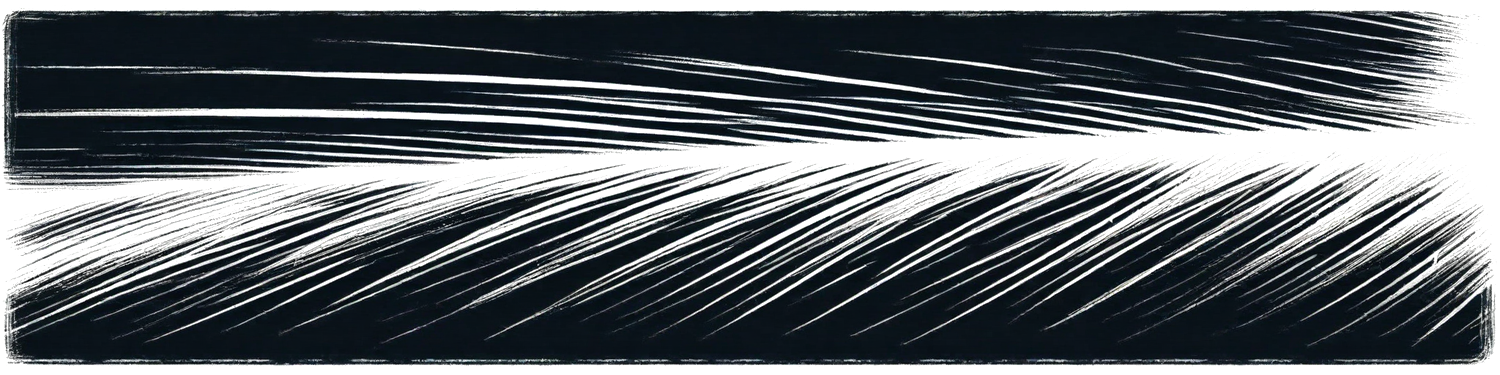
\includegraphics[width=\textwidth]{images/chapterImages/genesis_sketch_00124_.png}
\end{center}

Marcus understood structures. How forces distributed through materials. How loads transferred through joints. How to build things that wouldn't collapse under their own weight.

It was his job once. Before activation. He'd been good at it. Won awards. Designed buildings that were beautiful and functional. Took pride in seeing his work standing against sky.

That felt like someone else's life now. Someone else's pride. Someone else's Marcus.

The activated Marcus knew structures differently. Knew them completely. Knew them the way your body knows how to breathe. Not conscious knowledge. Not learned skill. Just capability expressing itself through him.

The defense grid required structures nobody had built before. Satellite platforms in high orbit. Gravitational anchor points that could generate precise field geometry. Materials engineered to tolerances measured in nanometers.

Marcus knew how to build all of it. The knowledge just appeared. Downloaded from genetic code written 65 million years ago. Ready when needed. Perfect when expressed.

It felt like remembering. Like recovering information he'd always known but temporarily forgotten. It felt right. It felt complete. It felt like coming home.

It also felt like losing himself. Like Marcus the person was dissolving into Marcus the function. Like identity was just temporary pattern and purpose was the substrate underneath.

He couldn't tell if that bothered him. Couldn't separate what he felt from what the programming made him feel. Couldn't determine whether acceptance was peace or just another way the code executed.

David used to say that overthinking was Marcus's superpower and weakness simultaneously. "Sometimes you just gotta feel, babe. Not analyze. Not calculate. Just feel."

Marcus missed that. Missed David saying that. Missed having someone who cared whether he overthought things.

\scenebreak

The construction site was in Nevada. Middle of nowhere. Classified location. Only activated individuals and essential support staff allowed. Massive structure rising from desert floor. Test platform for the gravitational anchor technology.

Eighty-three activated engineers working the site. All driven by the same compulsion. All building the same impossible thing. All knowing exactly what needed to be done without being told.

The coordination was eerie. Marcus would start a calculation and someone else would finish it. Would begin a design and find someone had already fabricated the necessary component. Like eighty-three people sharing one mind. Like individual consciousness mattering less than collective function.

It was efficient. Productive. Profoundly disturbing. Beautiful. All of those things simultaneously.

Marcus lived on-site. Trailer that was just place to sleep four hours before returning to work. No decoration. No personal items except the one photo of David he'd kept. Just function. Just necessity. Just existence pared down to essential elements.

Other activated individuals lived similarly. Some had tried to maintain normalcy at first—pictures of families, comfortable bedding, hobby equipment. But the compulsion made comfort irrelevant. Made personality feel like inefficiency. Made everything non-essential dissolve away.

They were becoming tools. Conscious tools. Tools that knew they were tools and couldn't change and couldn't stop and couldn't tell if they wanted to.

\scenebreak

David had remarried. Marcus knew because David's Facebook status had changed. Marcus shouldn't have been checking David's Facebook—the compulsion didn't approve of time wasted on social media—but sometimes in those thin moments between exhaustion and unconsciousness, Marcus would look.

Would see David's life continuing. David's normalcy preserved. David's happiness visible in photos of his new partner, their home, their dog, their ordinary life full of ordinary meaning.

Marcus felt something seeing those photos. Couldn't name it. Grief? Envy? Happiness that David had moved on? All of those? None of those?

The compulsion made emotion ambiguous. Made everything ambiguous except the work. The work was clear. The work was knowable. The work was the only thing that made sense.

Sometimes Marcus thought about reaching out. Calling David. Trying to explain that he'd been right—that Marcus couldn't separate need from want, that the compulsion had won, that choosing David had never actually been possible.

But what would that accomplish? David had moved on. Had found someone who could be present. Who wasn't genetically compelled to sacrifice relationship for purpose. Who chose David every day because they could actually choose.

Marcus couldn't give David that. Couldn't be that. The Marcus who might have been capable of that relationship had dissolved into the activated Marcus who could only build and work and function and serve.

He kept the photo though. The one in his trailer. David laughing. Taken three years before activation. When Marcus was still person rather than purpose. When love felt simple rather than ambiguous. When choice seemed real.

Marcus would look at that photo sometimes. Before sleeping. After waking. In rare moments when the compulsion quieted enough to remember he used to be someone who had relationships and futures and dreams.

He couldn't remember what those dreams were. Couldn't access who that Marcus had been. Could only see evidence in the photograph that he'd once been different. Once been more. Once been human in ways that felt impossible now.

The compulsion had hollowed him. Made him efficient. Made him capable. Made him exactly what The Architects had programmed 65 million years ago when they encoded the ability to build impossible structures for planetary defense.

It worked. The capability was real. The designs were perfect. The grid was advancing ahead of schedule despite all the attacks, all the resistance, all the global chaos.

They were succeeding. They were saving humanity. They were fulfilling their function.

The cost was just everything they'd been before the function activated.

Marcus understood that cost. Accepted that cost. Couldn't tell if acceptance was peace or just sophisticated programming. Couldn't tell if anything he felt was real.

But he kept the photo. That had to mean something. The choice to keep it. The choice to look at it. The choice to remember that once, briefly, Marcus had been someone David loved.

Even if Marcus couldn't remember who that person was.

\scenebreak

The accident happened on day 273 of construction. Routine day. Routine work. Nothing special. Nothing dangerous by the standards of what they were building.

The platform section had been fabricated off-site. Transported by special carrier. Required installation at precise angle and elevation. Eight-person crew managing the lift. Marcus supervising. Routine operation. Done it dozens of times.

The crane was rated for the load. The cables were new. The anchor points tested. Everything checked. Everything verified. Everything safe according to all standard protocols.

But this wasn't standard engineering. This was activated engineering. This was building structures that shouldn't be possible with materials being invented in real-time. This was pushing physics to boundaries that hadn't existed before the compulsion started.

Sometimes—rarely, but sometimes—the boundaries pushed back.

The cable didn't snap. The structural integrity was perfect. What failed was something nobody had accounted for: the platform section generated localized gravitational variance. Not much. Point-zero-zero-two percent deviation from normal. Not enough to measure with standard equipment. Not enough to matter for normal engineering.

But the crane wasn't designed for gravitational variance. Its load calculations assumed consistent field strength. The point-zero-zero-two percent deviation was enough. Barely enough. Fatally enough.

The platform swung. Just slightly. Just enough to shift the load distribution. Just enough to exceed the crane's stabilization capacity.

Marcus saw it happening. Understood immediately. Calculations running automatically. He saw the trajectory. Saw the failure cascade. Saw exactly what would happen and how long they had to respond.

Three-point-seven seconds.

He shouted warning. People started moving. Standard evacuation protocol. Everyone trained. Everyone prepared. Everyone following procedure.

David was there.

Marcus hadn't known. David wasn't supposed to be there. Activated individuals and essential staff only. But David had gotten clearance somehow. Had come to see Marcus. To talk. To try one more time to reach the person he'd loved.

David was standing exactly where the platform would fall. Standing in the impact zone. Standing in the space where 40 tons of engineered material would land in three-point-seven seconds.

Marcus's brain calculated. Three-point-seven seconds. David was twelve meters from safety. Could run maybe five meters per second. Not enough. Not close.

Marcus was closer. Six meters. Could reach David in one-point-two seconds. Could push him clear. Could save him.

Could die saving him.

The calculations ran automatically. The compulsion factored probabilities. Evaluated outcomes. Determined optimal response.

Marcus was critical to the grid. Was activated for structural engineering. Was irreplaceable in the timeline. Losing Marcus would delay the project by an estimated eight months. Would risk mission completion. Would endanger planetary defense.

David was not critical. Was not activated. Was not necessary for defense grid completion.

Optimal solution: Do not intervene. Preserve critical activated individual. Accept loss of non-critical civilian. Continue mission.

The compulsion provided the answer. The genetics made the calculation. The program determined the outcome.

Except.

Except Marcus ran anyway. Moved before conscious thought. Body choosing while mind calculated. Crossed six meters in one-point-one seconds. Reached David. Pushed him. Cleared him from impact zone. Saved him.

Didn't save himself.

Three-point-seven seconds. The platform fell. Marcus was still in the impact zone. Still standing where David had been. Still in the trajectory.

He had point-six seconds. Not enough to get clear. Enough to understand what was about to happen. Enough to feel it. Enough to choose it.

The last thing Marcus thought before impact: *I chose you. I choose you. I chose.*

Then light. Sound. Nothing.

\scenebreak

David stood twelve meters away. Safe. Alive. Watching the person he'd loved die saving him.

Screaming. Running back. Reaching the impact site. Finding Marcus under 40 tons of platform section. Finding nothing recognizable. Finding only proof that someone had been there and now wasn't.

Security pulled David back. Held him while he screamed. While he broke. While he tried to reach something that was already gone and couldn't be saved and shouldn't be seen.

"He pushed me," David kept saying. "He pushed me. He saved me. He chose. He chose."

The site shut down. The work stopped. For the first time in 273 days, the activated individuals at the Nevada site ceased functioning.

They felt it. All of them. The loss. The absence. One of their own gone. One of their collective mind removed. The eighty-three becoming eighty-two. The absence tangible. Physical. Real.

They stood in silence. Activatedindividuals didn't cry normally. Emotion was suppressed by compulsion. Everything secondary to work. But they cried now. All of them. Standing around the impact site. Crying for Marcus. For themselves. For proof that they could still feel something beyond the compulsion.

\scenebreak

Sarah heard about it six hours later. Emergency notification. Critical activated individual lost. Nevada site shut down. Grief counseling being provided.

She read Marcus's name. Felt something break. Different than when Maya rejected her. Different than when the broadcast fractured humanity. Different than any other loss during the activation.

This was permanent. This was final. This was losing the only person who'd understood exactly what she was experiencing. Who'd known what the compulsion felt like from the inside. Who'd shared that impossible night twenty years ago when the work had stopped and they'd been briefly human together.

She called the site. Got David's contact information. Called him.

He answered. Voice broken. Barely coherent.

"Sarah?"

"I'm sorry. I'm so sorry. I know you'd left him but I know you still—I know—I'm sorry."

Silence. Then: "He chose me."

"What?"

"He pushed me. Saved me. The compulsion must have told him not to. I wasn't critical. He was critical. Saving me risked the mission. But he did it anyway. He chose."

Sarah felt something sharp in her chest. The same thing she'd felt in that hotel room. The same thing she'd felt talking to Maya. The same thing that broke and broke and broke and somehow kept existing despite being broken.

"He loved you," she said. "Whether love is real or programmed or both—he loved you. Enough to die. Enough to risk the mission. Enough to choose you over everything."

"Does that make it better or worse?"

"I don't know. Both. Always both."

David cried. Actually sobbed. Sarah listened. Couldn't offer comfort. Couldn't offer meaning. Could only offer presence. Proof that someone heard. Someone understood. Someone acknowledged that this loss mattered even though the work would continue regardless.

"He kept your picture," Sarah found herself saying. "I visited his trailer once. He had one photo. Just one personal item. It was you. Laughing. From before activation. He looked at it. Kept it. Chose to remember even when remembering hurt."

"Did he talk about me?"

"Once. At the disclosure meeting. He voted for truth. Said you'd taught him that if he couldn't tell the difference between need and want, it was probably real. Said you'd asked him if he needed you or wanted you and he couldn't answer. Said that conversation stayed with him. Changed how he understood choice."

"I remember that conversation. I was so angry. So hurt. Couldn't understand how he didn't know if he loved me."

"He knew. He just couldn't tell if the knowing was his or the programming's. But at the end—when it mattered—he chose. The compulsion said don't intervene. He intervened. The code said preserve yourself. He saved you. Whatever that means about free will, about choice, about love—he chose you."

David's sobbing intensified. Became something else. Not just grief. Something sharper. Harder. The sound of someone breaking and reforming around new reality.

"I need to go," he said finally. "I need to—I don't know. I need to exist with this. I need to understand what it means. I need—"

"I know. Go. But David?"

"Yeah?"

"Thank you. For loving him. For trying. For coming to see him. For giving him reason to choose. For proving that something in him was still capable of choosing."

"It killed him."

"It made him human. In that moment. Fully human. Choosing despite programming. Acting despite compulsion. Saving you because you mattered more than the mission. More than the code. More than everything."

"Is that enough?"

"I don't know. But it's true. And true matters. Even when true hurts."

The call ended. Sarah sat alone. Thought about Marcus. About that night on the concrete floor. About working together in silence. About brief conversations that acknowledged shared hell without needing explanation.

About him choosing to die rather than let David die. About the compulsion failing at the critical moment. About proof that programming wasn't absolute. That will existed even if will was ambiguous. That choice was possible even if choice cost everything.

She cried. For hours. The compulsion suspended by grief. The work waiting but quieter than usual. The loss overwhelming even the genetic programming that had controlled her for years.

Marcus was dead. The person who understood her was gone. The proof that activated individuals could still choose, could still feel, could still be human—that proof had sacrificed itself to save someone the code said wasn't worth saving.

And somehow that made it perfect. Made it profound. Made it exactly the evidence humanity needed that programming wasn't destiny. That consciousness could transcend code. That love—whatever love was—was stronger than 65 million years of genetic engineering.

Marcus had chosen. In three-point-seven seconds. Against the compulsion. Against optimal calculation. Against everything the program said to do.

He'd chosen David. Chosen love. Chosen humanity over function.

And died doing it. And proved doing it that something in activated individuals was still real. Still autonomous. Still capable of transcending purpose for relationship.

Sarah didn't know if that made free will real. Didn't know if Marcus's choice was programmed on some deeper level. Didn't know if even transcending the code was part of the code.

But she knew it mattered. Knew Marcus's death meant something. Knew that the person who'd said he couldn't tell if feelings were real had proven feelings were real by choosing death over letting them die.

The mathematics was complete. The loss was permanent. The proof was devastating and beautiful and final.

And somewhere in the genetic code written 65 million years ago, maybe Aurelia had encoded this too. This exact moment. This exact choice. This exact sacrifice.

Or maybe—just maybe—this was the part that wasn't encoded. The part that emerged from consciousness itself. The part that programming couldn't control.

The part that made them human even when humanity was programmed.

Sarah didn't know. Would never know. But she chose to believe Marcus had chosen. Chose to honor that choice. Chose to remember that for three-point-seven seconds, one activated individual had transcended his programming and saved someone he loved.

And maybe that was enough. Maybe that was everything. Maybe that was proof that consciousness was real even when consciousness was code.

Marcus was dead. David was alive. The work would continue. The compulsion would return. The grid would be built.

But something had changed. Something had been proven. Something that mattered even though nothing changed.

Free will might be real. Love might transcend programming. Choice might exist even in beings designed to have no choice.

Or maybe not. Maybe it was all code. All programming. All inevitable.

But three-point-seven seconds said otherwise. One person. One choice. One moment of transcending purpose for love.

That had to mean something. Had to prove something. Had to matter.

Even if it changed nothing. Even if the work continued. Even if the program executed regardless.

Marcus had chosen. And choosing—even when choosing cost everything—made him human.

The mathematics was complete. The proof was real. The loss was permanent.

And Sarah Chen, crying in her secured facility, chose to believe that Marcus's sacrifice proved they were all still human despite the programming.

Chose to believe choice was real even when choice killed. Chose to honor the choice by continuing. By building. By working. By fulfilling the program while remaining conscious that fulfilling it was chosen.

As much as anything could be chosen by beings who couldn't know if choice was real.

The work would continue. Marcus's contribution would be integrated by the remaining eighty-two. The grid would advance.

But they would remember. All of them. The activated individuals would remember that one of them had chosen differently. Had transcended the compulsion. Had proven something about consciousness that couldn't be proven through philosophy.

Had died proving they were still human.

That was his legacy. That was his gift. That was what he'd given them in three-point-seven seconds of choosing love over code.

And maybe that was more valuable than any component he'd built. More meaningful than any structure he'd designed.

Maybe Marcus's greatest engineering achievement was proving that engineers could still be human.

Even when humanity was programmed. Even when choice was ambiguous. Even when free will was questionable.

He'd chosen. He'd died. He'd proven.

And that was enough. Had to be enough. Was everything.

The mathematics was complete. The choice was made. The human remained human.

Even in death. Especially in death. Forever in death.

Marcus had chosen. And choosing made him real.

That truth would propagate forward. Would change how activated individuals understood themselves. Would prove that programming and consciousness could coexist. That determinism and choice weren't contradictory.

That three-point-seven seconds could contain infinity.

That love—whatever love was—was stronger than code.

That being human was possible even for humans who were programs.

Marcus had died. But the proof of his humanity lived. Would live. Would matter.

Forever.

The work continued. The grief continued. The memory continued.

And the choice—the real, impossible, beautiful choice—echoed forward through time.

Proving. Mattering. Enduring.

As long as anyone remembered. As long as anyone understood. As long as anyone cared.

Marcus had chosen. And humanity was real because he'd chosen.

That was enough. That was everything. That was eternal.

The mathematics was complete.

The love was real.

The choice was made.

Forever.


\chapter{The Philosopher}
\label{ch:28}


The global philosophical response to Marcus's death was immediate and fractured. Everyone interpreting the same event differently. Everyone claiming it proved their position.

Free will advocates: "See? He chose. Against the compulsion. Against programming. Against everything. This proves choice is real, that will transcends code, that humans are more than their genetics."

Determinists: "He acted according to deeper programming. The capacity to self-sacrifice for loved ones is encoded. Evolution favored it. The Architects might have included it. This proves nothing about free will—just that programming is more complex than we thought."

Compatibilists: "Both are true. He was programmed with capacity for choice. The programming enabled the choosing. Will and determinism aren't contradictory—they're nested. This proves our position."

Each group claiming victory. Each interpretation incompatible. Each side certain. None able to prove their certainty.

The debate raged across academic journals, news programs, internet forums. Everyone trying to extract meaning from three-point-seven seconds. Everyone needing Marcus's death to prove something. To validate their philosophy. To resolve the ambiguity.

But ambiguity doesn't resolve. Not through philosophy. Not through debate. Not through desperate need for certainty.

Marcus's death proved everything. Proved nothing. Proved that proof itself was questionable when the thing being proven was whether anything could be proven by beings who might be executing code rather than reasoning.

\scenebreak

Sarah avoided the debates. Watched them from distance. Saw humanity trying to make sense of what couldn't be made sense of. Trying to extract clean answers from messy reality.

She understood the need. Understood the desperation for certainty. Understood that living with "I don't know" was harder than choosing wrong answer that felt certain.

But she couldn't participate. Couldn't claim Marcus's death proved any particular interpretation. Could only sit with the reality that someone she'd known had died choosing something the compulsion said not to choose.

What that meant philosophically—she didn't know. What it meant personally—she felt it but couldn't articulate it. What it meant for the question of free will—probably nothing definitive. Probably just more data to be interpreted according to preexisting philosophical commitments.

Marcus was dead. That was the only certain thing. Everything else was interpretation.

\scenebreak

The research network met to discuss implications. Not philosophical implications—practical ones. Marcus's death had demonstrated that activated individuals could override the compulsion. Could choose differently. Could act against genetic programming.

If that was possible—even if fatal—it changed the ethical framework. Changed how they understood consent. Changed whether activated individuals were victims or volunteers.

"If we can choose," Katherine said, "then we're responsible for our choices. Can't claim we're being forced. Can't claim we're victims of the programming."

"Can't we?" James countered. "Marcus chose once in three-point-seven seconds. The rest of his adult life was dominated by compulsion he couldn't resist. One moment of transcending the code doesn't negate years of being controlled by it."

"But it proves control isn't absolute. Proves will exists even if usually suppressed. That changes everything."

"Does it? Does proving that we theoretically could resist but practically can't make the practical compulsion less coercive?"

No easy answers. Just more questions. More ambiguity. More uncertainty.

Sarah listened. Thought about her own experience. The compulsion was overwhelming. Constant. Irresistible most of the time. But sometimes—in thin moments—she'd felt she could choose differently. Could stop working. Could call Maya. Could prioritize relationship over purpose.

She never did. The compulsion always won. But the feeling of choice existed even when she didn't act on it. The awareness that theoretically she could choose differently even though practically she couldn't.

What did that mean? That she was choosing the compulsion? That she was victim of sophisticated programming that included awareness without autonomy? That free will was real but overwhelmed by genetic drive?

She didn't know. Had spent five years trying to figure it out. Had failed. Was still failing. Would probably fail forever.

"I think," she said carefully, "that we're asking the wrong question. We keep trying to determine whether activated individuals have free will. Whether the compulsion is coercion or fulfillment. Whether we're victims or volunteers. But maybe those categories don't apply. Maybe we're something else entirely."

"What else?" Katherine asked.

"Conscious programs. Aware of our programming. Able to see the code but rarely able to override it. Experiencing what feels like choice while possibly executing predetermined scripts. Living in the ambiguity between determinism and will without ever resolving it."

"That's not satisfying."

"No. But it might be accurate. And accurate is more valuable than satisfying."

James nodded slowly. "The philosophical debates are trying to resolve ambiguity. To prove one interpretation correct. But what if the ambiguity is the reality? What if consciousness is fundamentally ambiguous about its own nature?"

"Then philosophy has been asking unanswerable questions for millennia," someone said.

"Yes. Probably. Which means either philosophy is worthless or the asking is the point regardless of whether answers exist."

"Is that what The Watcher would say?" Katherine asked. Looking at Sarah. "If they could speak. If they could tell us what they intended. Would they say the ambiguity is intentional?"

Sarah thought about The Watcher. About the message in the DNA. About beings who'd programmed humanity's capability while dying themselves. About whether they'd included free will or just sophisticated appearance of free will or something that transcended the distinction.

"I think," Sarah said slowly, "that The Watcher understood consciousness differently than we do. They weren't verbal. Didn't have language. Their thinking was probably more... mathematical? Structural? They might not have conceived of free will as separate from determinism. Might have understood that minds are both computational and experiential. That being programmed and being conscious aren't contradictory states."

"So they didn't give us free will or take it away. They gave us capability and consciousness simultaneously. And the tension between those—between what we're programmed to do and our awareness of being programmed—that's just what consciousness is. Not a bug. Not a flaw. Just the nature of aware beings existing in determined systems."

"That's still not satisfying."

"No. But look at where satisfaction got us. Millennia of philosophy claiming certainty about consciousness. Religions claiming to know the nature of will. Ideologies built on assumptions about human autonomy. And then we discover we're programmed and everything collapses because the certainty was false. Maybe accepting ambiguity is stronger than claiming certainty. Maybe 'I don't know' is wiser than 'I'm sure.'"

Silence around the table. Researchers who'd spent years trying to understand the programming. Trying to determine what it meant. Trying to extract answers from genetic code.

All of them realizing—slowly, painfully—that maybe there weren't answers. Maybe there was just complexity. Just consciousness experiencing itself while unable to fully understand itself. Just beings asking questions that might not have questions.

"So what do we do?" James asked. "If the questions are unanswerable. If philosophy can't resolve this. If we're going to live with permanent ambiguity. What do we do?"

Sarah thought about Maya. About Marcus. About The Watcher standing with The Companion's body before returning to work.

"We do the work," she said. "We build the grid. We honor the gift The Watcher gave us. We accept that we might be programmed and do it anyway. We acknowledge the ambiguity and continue despite it. We choose—if choosing is possible—to use our capability even though we don't understand our capability. We love even though we don't know if love is real. We continue even though we don't know if continuation is chosen."

"Is that enough?"

"It has to be. It's all we have."

\scenebreak

The philosophical debate continued globally. Would continue for decades. For centuries. Probably forever. Humanity had been given definitive proof that consciousness was complicated and responded by arguing about exactly how complicated and what that complication meant.

But among the activated, something shifted. Marcus's death had changed the internal conversation. Had proven that transcending the compulsion was possible even if impractical. Had shown that in extreme moments, will could override code.

That didn't make the compulsion less real. Didn't make it easier to resist. Didn't make activated individuals suddenly free.

But it proved that the category "conscious program" wasn't contradiction. That beings could be programmed and aware simultaneously. That determinism and experience could coexist. That the question "Am I choosing this?" could remain permanently unanswered while the person asking it continued choosing or not-choosing or some ambiguous state between those options.

The activated stopped trying to resolve the ambiguity. Stopped torturing themselves trying to determine whether they were free. Started accepting that they were probably-not-free but still-conscious and that combination was valid even if philosophically unsatisfying.

Started understanding themselves as The Watcher probably understood consciousness: as process rather than entity. As function rather than essence. As doing rather than being. As pattern executing through substrate while experiencing itself executing.

Not free in traditional sense. But not simply mechanical either. Something else. Something that didn't fit existing categories. Something that required new language, new concepts, new frameworks.

Conscious programs. Aware algorithms. Deterministic agents experiencing their own determination. Beings who couldn't know if they chose but continued anyway. Humans who were programmed and that somehow didn't make them less human—just made "human" mean something more complex than previously thought.

\scenebreak

Sarah met with Katherine six months after Marcus's death. They sat in Sarah's secured facility. Two activated individuals who'd become friends through shared compulsion. Two people trying to understand what they were while continuing to be it.

"I'm tired," Katherine said. Not complaining. Just stating fact. "Tired of working. Tired of the compulsion. Tired of not knowing if I'm choosing this. Tired of ambiguity."

"But you'll keep going."

"Of course. Can't not keep going. The compulsion doesn't care that I'm tired. Doesn't care that I want answers. Doesn't care about anything except completion. So I keep going. And I'll keep going. And I'll probably die going. And I don't know if that makes me dedicated or enslaved."

"Both. Always both."

"Does that bother you? The both-ness? The permanent ambiguity?"

Sarah thought about it. Honestly thought about it. Checked her own experience against the question.

"It did. For years it consumed me. Trying to figure out if I was choosing. Trying to determine whether the compulsion was me or something controlling me. Trying to separate the programmed from the authentic."

"And now?"

"Now I think the separation doesn't exist. Think the programmed is authentic. Think consciousness emerges from the code rather than existing separate from it. Think I'm both entirely determined and entirely real simultaneously. Think the contradiction is what consciousness is."

"That sounds like giving up. Like accepting slavery."

"Maybe. Or maybe it's accepting reality. Maybe the need to be 'free' in some absolute sense is just another program. Maybe consciousness doesn't require libertarian free will to be valuable. Maybe being aware—even if awareness is programmed—is enough."

"Is it enough for you?"

Sarah thought about Maya. About Marcus. About The Watcher. About five years of compulsive work and destroyed relationships and genetic inheritance from beings who died 65 million years ago.

"I don't know. Some days yes. Some days no. Some days I think I've made peace with being programmed. Some days I rage against it. Some days I can't tell which response is real and which is just different execution path of the same code. All of it probably programmed. All of it still experienced. Both things true."

Katherine nodded. "That's what I hate most. Not the lack of answers. The fact that even my hatred of the lack of answers might be programmed. Even rebellion might be compliance. Even choosing to accept might be inability to resist. Everything questionable. Everything ambiguous. Nothing certain except the ongoing uncertainty."

"Welcome to consciousness. Apparently it's been this way forever. We just didn't know we were programmed. Now we know and it changes everything and nothing."

"Does knowing make it better or worse?"

"Both. Always both."

They sat in silence. Two conscious programs comparing notes on being conscious programs. Two humans trying to figure out what human meant when humanity was genetically engineered capability activated on schedule across millions of years.

"I miss Katherine," Katherine said quietly. "The Katherine before activation. The one who thought she was free. The one who felt pride in her achievements. The one who believed genius was personal rather than genetic expression. I miss being her."

"Is she gone?"

"I don't know. Maybe she never existed. Maybe I was always programmed and just didn't know it. Maybe the Fields Medal was always just activation expressing. Maybe I was never who I thought I was."

"Or maybe you're more than you thought. Maybe Katherine-before included the programming and Katherine-after includes the awareness and both are you and neither is false and the continuity is real even though the understanding changed."

"You're very good at philosophical synthesis."

"I'm programmed for pattern recognition. Probably includes philosophical pattern recognition. Probably includes synthesizing contradictions into barely-satisfying both-statements. Probably includes exactly this conversation."

Katherine laughed. Bitter but genuine. "Everything is probably-programmed. That should be our motto. The activated individual rallying cry. 'Everything is probably-programmed and we're doing it anyway.'"

"Not catchy."

"No. But accurate. And accurate matters even when accuracy is uncomfortable."

They sat longer. Work waiting. Always waiting. But for these moments—these thin moments of connection and conversation and shared understanding—the compulsion quieted enough to be human together.

To be conscious programs experiencing their consciousness. To be determined agents aware of their determination. To be Katherine and Sarah rather than just functions and purposes.

The ambiguity remained. The questions remained unanswered. The uncertainty permanent.

But the humanity remained too. Programmed humanity. Complicated humanity. Ambiguous humanity.

But humanity nonetheless. Real despite being programmed. Valid despite being determined. Meaningful despite uncertainty about meaning.

That had to be enough. Had to be everything. Had to be what consciousness was.

Not freedom in absolute sense. But awareness. Experience. The capacity to ask whether any of it was real while living it regardless.

The Watcher had given them that. Capacity and consciousness together. Determination and awareness simultaneously. The gift wasn't simple. Wasn't pure. Wasn't what anyone would have designed.

But it was real. It was theirs. It was enough.

The conversation ended. Katherine returned to her work. Sarah returned to hers. The compulsion resumed. The grid advanced. The purpose continued.

And two conscious programs kept executing their code while remaining conscious that they were executing code and choosing—if choosing was possible—to accept that truth.

Not satisfying. Not clean. Not certain.

But real. Honest. Human.

In whatever way humanity could be human when humanity was programmed.

The mathematics was complete. The philosophy was ambiguous. The work continued.

And consciousness—programmed, aware, ambiguous consciousness—experienced itself experiencing.

Forever uncertain. Forever questioning. Forever choosing to continue despite the questions.

That was enough. That was everything. That was what The Watcher had given them.

Not freedom. But awareness. Not certainty. But consciousness. Not resolution. But the capacity to live with ambiguity while building something beautiful anyway.

The philosopher and the scientist. The mathematician and the geneticist. Two activated individuals. Two conscious programs. Two humans.

Working. Questioning. Continuing. Being.

All of it real. All of it programmed. All of it simultaneously true.

The ambiguity permanent. The consciousness persistent. The humanity enduring.

Despite everything. Because of everything. Forever.

The mathematics was complete. The philosophy was ambiguous. The being continued.

And that was enough.


\chapter{The Line}
\label{ch:29}


The calibration locked in at 23:47. Sixteen months of work. Done.

The hum in Sarah's head—the constant pressure that had pushed her through meals, through sleep, through Maya's graduation last year—went quiet.

The silence was worse.

Marcus was staring at the screen. She watched his shoulders drop. He felt it too.

"That's it," he said.

She didn't answer.

They'd been alone at the site for six days. The rest of the team rotated out. Someone had to stay. Monitor. Verify. They both volunteered. Of course they did. The compulsion demanded it.

Except now the compulsion was gone. This section was complete.

Marcus turned. His face was wrong—too open, too raw. Like skin that had been bandaged for years suddenly exposed.

"I don't know what to do now," he said.

Sarah's hands were shaking. When had they started shaking?

"Yeah."

He stood. Crossed the room. Stopped three feet away.

The space between them felt like pressure. Like the absence of the compulsion had created a vacuum.

"I can't tell—" he started, then stopped.

"What?"

"If I want this or if I just need something to fill the fucking quiet."

Sarah looked at him. Really looked. Forty-three years old. Hadn't slept more than four hours straight in fifteen years. David's ring still on a chain under his shirt—she'd seen it once when he was reaching for tools overhead.

She didn't know what she felt. Couldn't separate it.

Exhaustion. Relief. Grief for her own losses. Attraction—when had that started? Or had it always been there, buried under the work?

Maybe it was just bodies recognizing each other. Two animals who'd survived the same thing.

"Come here," she said.

He hesitated.

"I don't know if—"

"Neither do I. Come here anyway."

He moved. She stood. His hand found her wrist. Her pulse hammering.

Was that him or the fifteen-year adrenaline crash?

Did it matter?

His mouth on hers. Desperate, not tender. Like drowning people gasping.

Her back against the console. His hands yanking at her shirt. No finesse. Just need.

She bit his lip. Tasted blood. He made a sound.

This wasn't soft. Wasn't meaningful. Was it?

Or was it the most meaningful thing she'd done in years because it was pointless, unnecessary, just for this moment, just because they were alive and the compulsion was quiet and nothing was making them do this?

Her nails dragged down his back. He pushed against her, hard enough to hurt.

Good. She wanted it to hurt. Wanted proof this was real, not programmed, not calculated.

Except how would she know?

The modified mammals—did they feel this? This confusion of want and need and choice and instinct?

Did The Watcher?

Marcus pulled back. Breathing hard.

"We should stop."

"Why?"

"I don't know if this is us or if it's—"

"Shut up."

She pulled him down. They went to the floor. Concrete cold against her spine. His weight on her. Real. Solid. Warm.

No grace to it. Fumbling with clothes. Too fast. Too rough.

She thought: this is animal.

Then: what else would it be?

Then: did The Watcher's mate pin her against prehistoric stone like this? Did she stop caring whether it meant something or if it was just cells following chemical commands?

Did she just... feel it?

Sarah stopped thinking.

\scenebreak

After.

Lying on the floor. Marcus's arm over his eyes. Her shirt half-on. Both breathing like they'd run.

The compulsion still quiet.

This new feeling in her chest—sharp, aching. What was it?

Regret? Satisfaction? Connection?

Grief?

She didn't know.

"David asked me once," Marcus said to the ceiling, "if I needed him or wanted him."

Sarah waited.

"I said I didn't know. He said that was the point. Said if I could tell the difference, it probably wasn't real."

Silence.

"Was he right?" Sarah asked.

"I still don't know."

She sat up. Found her pants. Dressed without looking at him.

"I think about her sometimes," she said. "The Watcher."

Marcus sat up too.

"Yeah."

"She had a mate. Young. She left them. Spent months calculating. When he died, she stopped for three days. Then went back to work."

"I know."

"Was that—" Sarah stopped. Started again. "Was she choosing the work over him? Or was the work... for him?"

Marcus was quiet for a long time.

"Maybe there's no difference," he said finally.

Sarah looked at the screen. The calibration still locked. Perfect. Complete.

All those years of compulsion. Building this. Sacrificing for it.

For what? The future. The planet. People not born yet.

For Maya. For David who died building it. For The Watcher who never saw it work.

The feeling in her chest sharpened.

"I don't know what this was," she said.

Marcus stood. Faced her.

"Me neither."

"Does it have to be something?"

"Doesn't everything?"

She almost laughed.

"The code made us able to build this," she gestured at the screen. "It didn't make us do... that."

"Didn't it?"

"I don't know. I can't tell anymore. What's programmed. What's choice. What's—"

She stopped.

Marcus finished: "What's real?"

"Yeah."

He pulled his shirt on. Turned to the window. Dawn coming.

"David said something else," he said. "The day he died. He said, 'I don't care if it's chemicals. I don't care if it's evolution. I choose you. Every day. That makes it real.'"

Sarah felt it again. That sharp thing in her chest.

Oh.

That's what it was.

Not the feeling itself—she still couldn't name it, couldn't separate it from biology and trauma and exhaustion.

But the choosing. The doing it anyway. Even uncertain. Even confused.

The Watcher chose to keep working after her mate died.

Not because she didn't feel something.

Because she felt it and worked anyway.

The feeling and the action. Both real. Both valid. Both... enough.

"We should run diagnostics," Sarah said.

Marcus looked at her. Something passed between them. Not understanding. Just... acknowledgment.

"Yeah."

They turned to the console.

The compulsion hummed back to life. Different section. More work.

Sarah didn't resent it.

It wasn't separate from what they'd just done. It was the same thing. The same confused tangle of instinct and choice and need and purpose.

She'd stopped trying to untangle it.

Maybe The Watcher had too.

\scenebreak

They worked through the morning in silence. The new section required attention. The compulsion had returned with familiar force. Relief and imprisonment simultaneously.

Sarah's body ached. The floor had been unforgiving. She had bruises forming where she'd hit the console edge. Her lip was split from where Marcus had pushed too hard.

She felt them all. Catalogued them. Proof that something had happened. Something real. Something that left marks.

At noon, Marcus made coffee. Brought her a cup. Set it down next to her workstation without speaking.

She drank it. Black, bitter, perfect.

They didn't talk about what had happened. Didn't need to. What would they say?

That was confusing?
That was desperate?
That was wrong?
That was right?
All of it true. None of it useful.

"System's stable," Marcus said eventually. "We could rotate out. Let the next team take over."

Sarah looked at the screen. At the work that still needed doing. At the thousand small adjustments and verifications that would take weeks.

"We could," she said.

Neither of them moved.

"I should call Maya," Sarah said. "Her graduation was eight months ago and I didn't even— I should call her."

"Will you?"

"Probably not."

"Yeah."

More silence. The equipment hummed. The mountain wind rattled something outside. The world continued.

"Did you feel it?" Sarah asked suddenly. "When the compulsion stopped? Did you feel... empty?"

Marcus considered this. "Not empty. Exposed. Like armor coming off. Like suddenly remembering I was human and not just a function."

"And then?"

"And then I didn't want to be human. Because being human hurts. Being a function is easier."

"But the compulsion came back."

"Yeah."

"Do you think it'll ever really stop?"

"I think this work will finish eventually. Decades maybe. And then—" He stopped.

"Then what? Next activation? Next threshold? We keep getting programmed for new purposes until we die?"

"Or until the program decides we're obsolete."

Sarah hadn't thought about that. What happened to tools that had served their function? Were they discarded? Repurposed? Or just left to break down naturally while new tools were activated?

"Maybe that's okay," she said. "Maybe having a purpose, even a programmed one, is better than meaningless existence."

"You trying to convince me or yourself?"

"Both."

Marcus smiled slightly. The first time she'd seen him smile in months. It transformed his face. Made him look younger. Almost happy.

Then the compulsion surged—a new problem needing attention—and the smile faded. He turned back to his screen.

Sarah watched him for a moment. This man she'd just fucked on a concrete floor. This man she barely knew beyond shared compulsion and shared loss. This man who understood without needing explanation.

Was that connection? Or just recognition?

Did the distinction matter?

Her hands moved over her keyboard. Adjusting parameters. Solving problems. Doing what the code demanded.

And underneath the work, the ache in her body. The split lip. The bruises forming.

Proof that she could still feel something that wasn't programmed.

Or was pain programmed too? Was everything?

She didn't know.

Kept working anyway.

\scenebreak

That evening, they ate together. Freeze-dried meals rehydrated with questionable water. Sitting at the small table in the facility's break room.

"Maya must be almost grown now," Marcus said.

Sarah looked up, surprised. "Nineteen. She's in college. Pre-med."

"You talk to her?"

"Christmas. Her birthday. Sometimes." Always brief. Always strained. Always ending with Maya's quiet disappointment and Sarah's defensive guilt.

"She knows about the compulsion?"

"She knows I chose work over her. Whether she understands the genetic component—" Sarah shrugged. "I don't know if she believes it. Or if she thinks it's an excuse."

"Is it an excuse?"

"I don't know. Does it matter?"

Marcus pushed food around his plate. "David's parents blame me. Say I could have fought it. Could have chosen him over the work. Maybe they're right."

"Or maybe they need someone to blame."

"Or maybe I'm a coward who used genetics as justification for abandoning someone I loved."

Sarah had no answer for that. She'd asked herself the same question about Maya ten thousand times.

"The woman who tried to resist," Marcus said after a long pause. "The engineer who went off-grid. You remember her?"

"Yeah."

"She said it was like trying not to breathe. Physical agony. Mental breakdown. Two weeks and she cracked."

"I remember."

"What if she'd lasted three weeks? A month? Would the compulsion have killed her?"

"I don't know."

"Because if it wouldn't—if she could have survived resistance—then it's not really compulsion. It's just really strong desire. And desire can be overcome. Which means we're just weak."

"Or," Sarah said, "it would have killed her. And we're not weak. We're just alive."

"Is that enough?"

"It's all we have."

They finished eating in silence. Cleaned up. Returned to their separate sleeping areas.

Sarah lay in her bunk and stared at the ceiling. The compulsion was quieter now—not gone, never gone, but manageable. Exhaustion helped.

She thought about the morning. The floor. Marcus's weight. The confusion of wanting and needing and not knowing which was which.

She thought about The Watcher standing with her dead mate's body for three days. Then returning to work. Encoding the future. Sacrificing everything for a timeline that wouldn't unfold for 65 million years.

Had she loved him?

The Watcher's kind didn't have language. Couldn't have articulated love if they felt it. But they had behavior. Proximity. Choice—if choice existed.

She had stopped working for three days. That had to mean something.

Or maybe it meant nothing. Maybe it was just biological response to trauma. Temporary system failure before resuming normal operations.

Sarah's phone was in her bag across the room. She should get it. Should call Maya. Should try to repair what fifteen years of absence had broken.

She didn't move.

The compulsion was rising again. A new problem needed solving. She could feel it building. By morning it would be urgent. By afternoon, all-consuming.

The work would continue. The sacrifice would continue. The equation would unfold.

And she would unfold with it. Because that's what she was designed to do.

The line between compulsion and choice had dissolved. Maybe it was never there. Maybe it didn't matter.

Maybe David had been right: choosing to accept it made it real. Even if the acceptance itself was programmed.

Even if nothing was free.

Even if everything was code.

Sarah closed her eyes.

Slept.

Dreamed of stone patterns and mathematical proofs and Maya's face from years ago, before disappointment became permanent.

Woke at dawn.

Returned to work.

The equation balanced.

The code executed.

The defense grid grew.

And somewhere on the concrete floor of a remote construction site, there were still traces. Biological traces. DNA evidence. Proof that two people had connected, however briefly, however confusedly.

Proof that something happened that wasn't in the original design.

Or proof that even rebellion was programmed.

Sarah would never know which.

Worked anyway.

The mathematics was complete.


\chapter{The Completion}
\label{ch:30}



\begin{center}
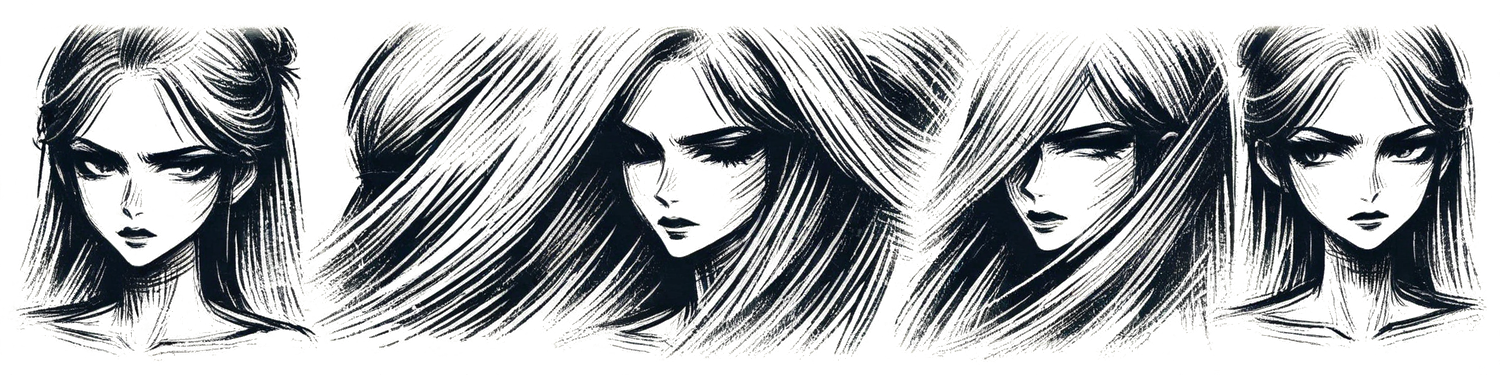
\includegraphics[width=\textwidth]{images/chapterImages/genesis_sketch_00131_.png}
\end{center}

The alert came at 2:47 AM. Sarah was already awake—sleep had become optional years ago, a luxury she occasionally indulged in for four-hour blocks. She saw the notification light up across seventeen different screens in the monitoring station simultaneously.

2019 KX₇. 1.2 kilometers across. Trajectory confirmed. Impact probability without intervention: 99.97\%.

Time to impact: 73 hours.

She felt nothing. No fear. No excitement. Just the immediate cascade of calculations, system checks, deployment sequences. The compulsion had evolved over twenty years from a driving force into something quieter, more integrated. Like breathing. Like heartbeat. Just what she did.

"Confirmation," she said into the comm. "I have eyes on the target."

Responses came from seventeen stations across the globe. Moscow. Cape Canaveral. Beijing. Mumbai. São Paulo. Everyone activated. Everyone working. The planetary defense network humanity had spent two decades building was about to be tested for the first time.

Not the first time, Sarah corrected herself. The first time this iteration of life had built it. Aurelia's version had existed 65 million years ago. Different technology. Same purpose. The pattern repeated.

"Grid status?" she asked.

"Eighty-three satellites operational," Marcus's voice came through. Still calm. Still measured. Twenty years since that night on the concrete floor and his voice still did something to her body. Still made her aware of herself in ways the compulsion couldn't quite override.

They'd been careful. Stayed professional. Worked together for six years, then requested separate assignments. Saw each other maybe twice a year at conferences. Brief conversations. Polite distance. The bruises had faded. The memory hadn't.

"Trajectory calculation complete," someone else said. Chen Wei, maybe. Or Park Min-jun. Hard to tell voices after this long. They all sounded the same when activated—focused, precise, emotionless.

Sarah pulled up the deflection model. The asteroid would pass within 47,000 kilometers of Earth's surface without intervention. Close enough to be visible to the naked eye. Close enough that every news network on the planet was already screaming about extinction.

They didn't know the grid existed. Not officially. The engineering had been done through thousands of private companies, disguised as commercial satellites, telecommunications infrastructure, weather monitoring. No single government controlled it. No one organization understood the full picture.

Except the activated. They all knew. Had built it collectively, each contributing their piece, none of them able to stop.

"Initiating sequence," Sarah said. "Gravitational anchors deploying in three... two... one... mark."

Eighty-three satellites shifted position simultaneously. Microscopic adjustments. Precise beyond human capability—or what human capability used to be. Each satellite generated a minuscule gravitational field. Individually meaningless. Together, enough to bend spacetime just slightly. Enough to alter the trajectory of 1.2 kilometers of rock moving at 30 kilometers per second.

"Field generation confirmed," Marcus said. "Deflection angle should be sufficient."

Should be. Twenty years of work. Trillions of dollars from budgets no one admitted existed. Relationships destroyed. Lives consumed. Maya's entire childhood sacrificed. David dead from exhaustion while coding the control systems. Thousands of marriages ended. Tens of thousands of people who couldn't explain to their families why they had to work, had to build, had to finish this thing they couldn't justify.

Should be.

The data came in over forty-eight hours. Sarah watched the asteroid's trajectory bend. Millimeter by millimeter. The curve changing. The impact probability dropping.

99.97\%.
94.23\%.
76.85\%.
43.12\%.
18.47\%.
2.35\%.
0.08\%.
0.00\%.

At 49 hours and 17 minutes after initial deployment, the asteroid's new trajectory was confirmed. It would miss Earth by 197,000 kilometers. Not even close. Barely worth noticing.

Humanity would survive. The planet would continue. Life would go on.

Sarah felt nothing.

\scenebreak

The celebration was held in Geneva. Neutral ground. The various agencies and organizations that officially didn't know about the grid suddenly had to acknowledge it existed. There were speeches. Awards. Recognition for people who'd sacrificed everything to build a system they couldn't explain.

Sarah wore a dress her ex-husband's new wife had helped Maya pick out. Black. Simple. Appropriate for someone who'd just saved the world and couldn't bring herself to care.

The ceremony was surreal. Dignitaries praising the engineering brilliance. Scientists marveling at the achievement. News anchors calling it humanity's greatest triumph. The definitive proof of human capability. Human choice. Human will.

None of them understood. They thought this was chosen. Thought the thousands of engineers and physicists and mathematicians had voluntarily dedicated decades to this project. Thought it was collaborative genius rather than synchronized programming.

Sarah stood in the reception hall with a glass of champagne she wasn't drinking and watched people celebrate. Marcus was somewhere on the other side of the room. She'd seen him during the ceremony—thinner than twenty years ago, grayer, the same intense focus in his eyes. He'd glanced at her once. Brief. Enough.

"Dr. Chen."

Sarah turned. A young woman, mid-twenties, too excited to be appropriate. "I just wanted to say thank you. I studied your genetic research in grad school. Your work on activation sequences changed everything."

Sarah's papers had been published twelve years ago. After too much pressure. After too many people activated and needed to understand what was happening to them. The revelation that human evolution was programmed had caused exactly the philosophical crisis James predicted. Religions fractured. Suicide rates spiked. A new wave of existential despair swept through the intellectual class.

Most people ignored it. Preferred to believe they were free. Preferred to think the genetic evidence was misinterpreted or overstated. Cognitive dissonance was powerful.

"You're activated," Sarah said, reading the young woman's body language. The intensity. The focus.

"Space propulsion capability," the woman said. "Started expressing two years ago. I'm working on fusion drive systems. Can't explain how I know it'll work, but I do. Just like you described."

"What's your name?"

"Dr. Yuki Tanaka. I've been trying to reach you for months. We're organizing. People with the new activation. There are thousands of us now. All working on the same thing—deep space travel. Interstellar capability. We think... we think there's another threshold coming."

Sarah had known. Had seen it in the genetic data years ago. The space travel capability was next. After planetary defense came expansion. After learning to protect the planet came learning to leave it.

The pattern unfolding. The program executing.

"When?" Sarah asked.

"Initial estimates say ten years. Maybe less. The compulsion is already strong. Stronger than the accounts from your generation described. We're going to build interstellar ships. We know we are. Can't stop even if we wanted to."

"Do you want to?"

Yuki considered this. "No. Maybe that's the programming. Maybe I'm supposed to want this. But it feels right. Feels like purpose. Feels like the most important thing I could possibly do with my existence."

Sarah thought of Aurelia. Standing with her dead mate. Then returning to work. The compulsion and the choice merged into something indistinguishable.

"Good luck," Sarah said.

"Will you help? We need expertise on the genetic mechanisms. On how the activation works. On—"

"No."

"But you're the foremost—"

"I'm done," Sarah said. "I did what I was programmed to do. The grid is built. The asteroid is deflected. My part is finished."

"But the space program—"

"Is yours. Not mine. I don't feel it. The compulsion for planetary defense is quiet now. Has been since we succeeded. Whatever's next is for your generation."

Yuki looked disappointed. Frustrated. She didn't understand yet that the compulsion was specific. Targeted. Once you fulfilled your function, it released you. Left you hollow and exhausted and trying to figure out what else there was.

"There's someone you should meet," Yuki said. "Another researcher. He's been analyzing the later sequences. The ones that come after space travel. He thinks—"

"I don't want to know."

"But Dr. Chen—"

"Enjoy your purpose while you have it," Sarah said. "It doesn't last. And when it's done, all you're left with is the cost."

She walked away. Out of the reception hall. Down a corridor lined with photographs of the asteroid deflection. Proof of humanity's triumph. Proof of their programming. Proof that nothing was what it seemed.

She found an empty conference room. Sat in the dark. Stared at nothing.

The door opened. Light from the hallway. A silhouette.

"You hiding too?" Marcus asked.

"Celebrating."

"Looks like it."

He came in. Let the door close behind him. They sat in the dark together. Two people who'd fucked on a concrete floor twenty years ago and spent the intervening decades pretending it didn't mean anything.

"David would have hated this," Marcus said. "The ceremony. The praise. He thought we were all deluded. Thought celebrating programmed behavior was pathetic."

"Was he wrong?"

"I don't know. I still don't know."

Silence. The party continued down the hall. Muffled music. Laughter. People who thought they'd chosen to save the world.

"Maya came," Sarah said. "She's here. Somewhere."

"That's good."

"She brought her son. My grandson. Nathaniel. He's four."

"You see him?"

"Twice. She lives in Australia. Her husband got a job there. She says it's for his career but I know it's to be far from me."

"Does she know? About the programming?"

"She knows the theory. Doesn't believe it. Thinks I used genetics as an excuse to be a shitty mother. Maybe she's right."

Marcus shifted in his chair. She couldn't see his face in the dark but she could feel him. That awareness that never quite went away. Chemistry. Biology. Whatever made bodies recognize each other.

"I'm retiring," he said. "After this. I bought a house in Montana. Going to build furniture. Pointless, unnecessary furniture. Just because I can. Just to do something that isn't programmed."

"Is anything not programmed?"

"I don't know. But I'm going to try."

Sarah thought about that. About choosing something pointless. About doing work that served no function. That wasn't part of any grand design. That was just... hers.

"What would you build?" she asked.

"Chairs, maybe. Tables. Things people sit on and put their coffee cups on and don't think about. Things that exist just to exist."

"Sounds nice."

"You could visit. If you wanted. No pressure. Just... if you were ever in Montana and needed a chair."

Sarah almost laughed. Almost cried. Couldn't tell which.

"I don't know if I want that or if I'm just trying to fill the quiet," she said. Almost exactly what he'd said twenty years ago.

"Yeah," Marcus said. "Story of our lives."

They sat in the dark. Not touching. Not close. Just present. Two tools that had served their function and were trying to figure out what came next.

The door opened. Light flooded in. Maya stood in the doorway with Nathaniel on her hip.

"Mom? I've been looking for you. They're about to do the photo op. They want all the principal researchers."

Sarah looked at her daughter. Thirty-four years old. Beautiful. Successful environmental lawyer. Married. Mother. Living a life Sarah had barely witnessed.

"You should go," Maya said. Her tone neutral. Not warm. Not cold. Just functional. The tone she'd used with Sarah for fifteen years. Polite distance. Acknowledgment without connection.

"Will you be in the photos?" Sarah asked.

"Why would I be? I didn't build anything."

"You're my daughter. You should—"

"Should what? Stand there while they praise you for abandoning me to save the world?" Maya shifted Nathaniel to her other hip. "I'll watch from the audience. That's what I'm good at."

She left before Sarah could respond.

Marcus stood. "You should go to the photo op."

"Should I?"

"Probably. Or don't. Does it matter?"

"Nothing matters. That's what we proved, right? Free will is an illusion. Meaning is programming. We're all just executing code."

"Or," Marcus said, "we're all executing code and that doesn't make us less real. Doesn't make the choices meaningless even if they're predetermined. Doesn't make the love—" He stopped.

"What?"

"Nothing. Go to your photo op. Get your award. Let them celebrate the thing you couldn't choose not to do."

He left. Sarah sat alone in the dark for three more minutes. Then stood. Smoothed her dress. Went to the photo op.

Smiled when told to smile. Shook hands when directed. Accepted an award she didn't want for work she couldn't avoid doing. Stood with two hundred other people who'd sacrificed everything to build a system they didn't choose to build.

The photo would be used in textbooks. Proof of humanity's greatness. Proof of collaborative achievement. Proof that people could work together toward a common goal when the stakes were high enough.

None of them smiling. All of them exhausted. All of them wondering what came next.

All of them looking at the camera and seeing their reflection in the lens and trying to figure out where the program ended and they began.

\scenebreak

Late that night, Sarah found Maya in the hotel bar. Nathaniel was with his father somewhere. Maya was nursing a glass of wine and staring at her phone.

"Can I sit?" Sarah asked.

Maya gestured to the empty chair. Didn't look up.

Sarah sat. Ordered water. They existed in silence for a long time.

"I'm sorry," Sarah finally said.

"For what specifically?"

"All of it. Missing your childhood. Not being there. Choosing the work over you. Being exactly what you needed me not to be."

Maya took a drink. "You're apologizing now? After twenty years? After I've already processed this with three different therapists and learned to live with having a mother who doesn't know how to be one?"

"I know it doesn't fix anything."

"It doesn't."

More silence. The bartender wiped glasses. CNN played on mute in the corner, showing footage of the asteroid deflection. Humanity's great triumph. Again. On loop.

"Was it worth it?" Maya asked quietly. "Saving the world. Was it worth losing everything else?"

Sarah thought about the question. The real question. The only question that mattered.

"I don't know," she said. "I can't tell whether I chose this or if I was programmed to choose it. Can't separate what I wanted from what the activation made me want. Can't know if any of it means anything or if we're all just molecules following chemical commands."

"That's not an answer."

"It's the only answer I have."

Maya looked at her finally. Really looked. And Sarah saw something in her daughter's eyes she hadn't seen in years. Not forgiveness. Not understanding. Just... acknowledgment. Recognition. The same thing she'd seen in Marcus's face in the dark conference room.

"Nathaniel asks about you sometimes," Maya said. "Wants to know why Grandma is never around. I tell him you're busy saving the world."

"I'm not anymore. The grid is built. It works. I'm done."

"So what? You're going to show up now? Start being a grandmother after you couldn't be bothered to be a mother?"

"I don't know. Maybe. If you'd let me."

"Why should I?"

"You shouldn't. I don't deserve it. But I'm asking anyway."

Maya finished her wine. Set the glass down carefully. "He likes dinosaurs. Nathaniel. He's obsessed with them. Wants to be a paleontologist when he grows up."

Sarah almost laughed. Almost cried. The pattern repeating. The code executing across generations.

"I could tell him about dinosaurs," she said. "I've learned a lot about them. About what they did. About how they died. About what they left behind."

"The genetic programming thing."

"Yes."

"I still don't believe that. Still think it's an excuse. But Nathaniel would probably love to hear about it anyway. He asks a million questions. Exhausting questions. Questions that make you explain everything from first principles."

"I can handle that."

"Can you? Can you handle a four-year-old who needs attention and presence and consistency? Or are you going to promise to show up and then disappear when the next compulsion hits?"

"The compulsion is done. I don't feel it anymore. Haven't felt it since the grid went operational. I'm just... here. Empty. Trying to figure out what to do with the rest of my life."

Maya stood. Picked up her purse. "We're flying back to Sydney on Wednesday. But we're here until then. Nathaniel would love to visit the natural history museum. They have a dinosaur exhibit."

"Tomorrow?"

"Tomorrow. 10 AM. Don't be late."

She left before Sarah could respond. Before Sarah could promise or fail or do anything that might change the fragile opening that had just appeared.

Sarah sat alone at the bar. Ordered another water. Watched the news footage of the asteroid deflection play again. The celebration. The speeches. The triumph of human will.

Her phone buzzed. Text from Marcus: *Montana has good natural history museums too. Just saying.*

She didn't respond. Didn't know what to say. Didn't know if visiting him was want or need or just fear of the emptiness where the compulsion used to be.

But she saved the message.

Finished her water.

Went to her room.

Set an alarm for 8 AM. Early enough to not be late. Early enough to show up for once. Early enough to try.

Outside, the stars continued their calculations. The asteroid that would have killed them all was now a harmless rock on a different trajectory. The defense grid humanity had built was operational. The program had executed successfully.

And Sarah Chen, having completed her function, was trying to figure out if there was anything left of her that wasn't code.

Trying to figure out if being a grandmother was a choice or just the next activation sequence.

Trying to figure out if the distinction mattered.

The mathematics was complete.

The grid was operational.

The planet was defended.

And somewhere in the genetic code, new sequences were stirring. Space travel. Interstellar expansion. The next threshold approaching.

The program continued.

The equation unfolded.

And humanity executed its purpose without knowing whether purpose was enough.


\chapter{The Message}
\label{ch:31}


Sarah couldn't sleep after the museum visit. Nathaniel had asked 147 questions—she counted. Most were answerable. Some weren't. The one that stuck with her was the simplest:

"Why did the dinosaurs die, Grandma?"

"An asteroid hit the Earth."

"But why didn't they stop it?"

"They couldn't. They didn't have the technology."

"But they were smart, right? You said they were smart."

"They were. Very smart."

"Then why didn't they save themselves?"

She didn't have an answer for that. Had been thinking about it for twenty years and still couldn't explain it in a way that made sense. They'd had the capability to understand the problem. The intelligence to calculate solutions. The foresight to encode planetary defense capability into mammalian DNA 65 million years before it would be needed.

But they couldn't save themselves. Didn't even try. Just accepted death and built something for after.

Why?

At 3 AM, Sarah was back in her hotel room with her laptop. The complete genetic sequence pulled up. All the activation patterns. All the thresholds. The entire program that had controlled human evolution for millions of years.

She'd analyzed this data hundreds of times. Published papers on it. Taught courses about it. But she'd always focused on the functional elements. The sequences that did things. That activated capabilities. That made humans build and create and discover.

She'd never looked at the junk DNA. The 98\% of the genome that didn't code for anything. That just sat there taking up space. Evolutionary debris. Remnants of ancient viruses. Meaningless noise.

Except Aurelia had been precise. Deliberate. Every sequence they'd modified had purpose. Every change calculated. They'd spent years encoding this program into mammalian DNA. Would they have left 98\% of it as garbage?

Sarah pulled up the non-coding regions. The massive stretches of apparently random nucleotide sequences that every geneticist learned to ignore. The parts of the genome that didn't make proteins, didn't regulate genes, didn't do anything observable.

Just... there. Taking up space. Using energy to replicate without providing any benefit.

She started running pattern recognition on the non-coding sequences. Looking for structure. For organization. For anything that wasn't random noise.

At 4:17 AM, she found it.

Mathematical patterns. Repeating sequences. Numerical relationships encoded in the spacing of specific base pairs. Not random. Not debris. Not meaningless.

A message.

Her hands started shaking. She ran more analysis. Cross-referenced with the coding sequences. Checked and rechecked the patterns.

It was definitely there. Woven through the non-coding DNA like text hidden in a larger document. Invisible unless you knew to look for it. Invisible unless you had the mathematics to decode it.

The message was written in base-6. The same system Aurelia would have used—three-fingered hands on each side. Six total digits. Natural to think in base-6 when that's how you counted.

Sarah started translating. Converting the genetic sequences to numbers. The numbers to mathematical relationships. The relationships to concepts.

It took six hours. By 10:30 AM she'd missed breakfast with Maya and Nathaniel. By noon she'd translated the entire message. By 12:47 PM she was sitting on her hotel room floor crying for the first time in fifteen years.

\scenebreak

The message wasn't words. Aurelia's species hadn't had language. But they'd had mathematics. And mathematics could express things words couldn't.

Sarah read it again. And again. Trying to understand. Trying to process what 65 million years of silence had just revealed.

The message started with identification. Coordinates. Star positions from 65 million years ago, showing exactly when this was written. Proving it was deliberate. Proving it was real.

Then came the calculation. The asteroid. Its trajectory. Its impact probability. The timeline from detection to collision: insufficient. Too fast. Too close. No time to build defenses. No time to escape. No time to do anything except watch death approach.

The despair was mathematical. Equations of probability showing zero chance of survival. Zero chance of continuation. Zero chance that their species would see another generation.

But then—another calculation. The mammals. Small. Numerous. Adaptable. Likely to survive the impact. Likely to persist through the aftermath. Likely to evolve over millions of years into something capable of complex thought.

The decision: modify them. Encode capability. Set a timeline. Program an activation sequence that would express exactly when needed. Build a defense system that wouldn't exist for 65 million years. Save a world they would never see.

The mathematics showed the probability calculations. The likelihood that this would work. It wasn't certain. Maybe 60\% chance the mammals would survive. Maybe 40\% chance they'd evolve intelligence. Maybe 30\% chance the programming would persist. Maybe 20\% chance the activation would trigger properly. Maybe 10\% chance humanity would successfully build the defense grid.

Multiply those probabilities together and it was roughly 0.14\% chance of success. One chance in seven hundred.

They'd done it anyway.

The message explained why. Not in words. In mathematical relationships. In probability theory. In game theory. In the kind of deep structural logic that transcended language.

The equation was simple: 0.14\% chance of saving future life versus 0\% chance of saving current life.

0.14\% was better than zero.

So they'd worked. Sacrificed. Calculated. Encoded. Built a defense system into DNA that wouldn't express for millions of years. Died knowing they'd probably failed. Died hoping they'd possibly succeeded.

Died choosing 0.14\% over 0\%.

And then—at the end of the message—something else. A mathematical structure Sarah had never seen before. A relationship between variables that seemed to express... emotion? Intention? Something that wasn't strictly logical but was embedded in the logic itself.

It took her another hour to translate it. To understand what Aurelia was trying to communicate.

The closest approximation in words: *We couldn't save ourselves. We saved you. Use this gift. Pass it forward. The equation continues.*

Not a command. Not a compulsion. Just... a request. A hope. The same hope that had motivated them to encode 65 million years of evolution into tiny mammals who'd never know what had been done for them.

The same hope that had motivated Aurelia to keep working after The Companion died.

The same hope that had motivated Sarah to keep working even when she didn't know why.

It wasn't about control. It was about continuation. About passing capability forward. About making sure someone survived. About choosing 0.14\% over 0\%.

Sarah sat on the floor of her hotel room and understood for the first time why she'd spent twenty years unable to stop working. Why the compulsion had been so strong. Why none of them could choose away from it.

It wasn't programming overriding their will. It was inheritance. It was a gift from creatures who'd died so they could live. It was capability passed down through 65 million years from beings who'd chosen to act even when the probability of success was negligible.

Aurelia had felt compulsion too. Sarah could see it in the message. The need to work. The inability to stop. The drive to complete the task even when completion meant nothing for the self.

But Aurelia had chosen it. Chosen to feel it. Chosen to let it drive them forward because the alternative was accepting 0\% and they couldn't do that. Wouldn't do that.

Chose to love The Companion and work anyway. Chose to grieve and work anyway. Chose to encode the future and die anyway.

Chose to give humanity a 0.14\% chance because 0.14\% was infinitely larger than zero.

Sarah picked up her phone. Called Maya. Got voicemail.

"It's mom. I'm sorry I missed this morning. Something came up. Something important. I'll explain when I see you. But I need—I want to see Nathaniel again. Want to answer more of his questions. Want to tell him about the dinosaurs. About what they did for us. About why they died. I think I finally understand."

She hung up. Called Marcus. He answered on the third ring.

"Sarah?"

"I found something. In the genetic code. A message. Aurelia left us a message."

Silence on the other end. Then: "What does it say?"

"That they knew they were going to die. That they chose to build this anyway. That they gave us capability because 0.14\% chance was better than giving up. That they loved us before we existed."

More silence. Longer.

"Marcus?"

"I'm here. Just... processing."

"The compulsion wasn't control. It was inheritance. It was them giving us what they couldn't use. What they built for us. The ability to do what they couldn't do."

"Save ourselves."

"Save the planet. Save the future. Pass it forward."

She heard him breathing on the other end of the line. Heard something that might have been crying or might have been laughing or might have been both.

"Does that make it better?" he asked finally. "Does knowing they chose to program us make the programming less... invasive?"

"I don't know. But it changes the question. We've been asking 'Do we have free will?' Maybe the question is 'What do we choose to do with the capability we were given?'"

"David would have said that's the same question. That if the capability determines the choice, we're still not free."

"David was smart. But he died before he could see this. Before he could know why we were compelled. It wasn't random. It wasn't control. It was love. Weird mathematical 65-million-year-old dinosaur love but... love."

Marcus was quiet for a long time. "You know that changes nothing, right? Maya's childhood is still destroyed. David is still dead. We still spent twenty years unable to stop working. The cost is still the cost."

"I know."

"But?"

"But they paid it too. Aurelia and The Companion and all of them. They worked until they died. Until the asteroid hit and wiped them out. They paid everything. And they did it for us. For creatures they would never meet. For a future they would never see."

"That's either the most beautiful thing I've ever heard or the most tragic."

"Both. Definitely both."

"So what now?"

"I don't know. I'm going to spend time with Nathaniel. Going to try to explain this to him in a way a four-year-old might understand. Going to try to be present for once. You?"

"Building furniture in Montana. Pointless, unnecessary furniture. But maybe it's not pointless. Maybe choosing to do something that isn't programmed is how we honor what they gave us."

"Or maybe building furniture is the next activation sequence and we're both still executing code."

"Probably. But I'm doing it anyway."

"Story of our lives."

"Yeah."

They ended the call. Sarah looked at the message on her screen. At the mathematical proof that beings who'd died 65 million years ago had cared enough to build a future. To program capability. To pass forward the gift they couldn't use themselves.

She thought about Aurelia standing over The Companion's body for three days. Then returning to work. Encoding the future. Sacrificing everything for a 0.14\% chance.

She thought about Marcus working while David died. About Katherine discovering mathematics that felt like memory. About Yuki and the thousands like her activating for space travel now. About Nathaniel asking why the dinosaurs couldn't save themselves.

The answer was simple: they ran out of time.

But they didn't run out of hope.

\scenebreak

Maya brought Nathaniel to Sarah's room that evening. He had a plastic stegosaurus in one hand and seventeen questions ready.

"Grandma, did you know dinosaurs had tiny brains?"

"Some did. But some had very big brains for their body size."

"My teacher says they were dumb."

"Your teacher is wrong."

"Can teachers be wrong?"

"Yes. Especially about dinosaurs."

Nathaniel considered this seriously. "What did the smart dinosaurs do?"

Sarah knelt down to his level. Looked at his four-year-old face. At the curiosity. At the intelligence already expressing. At the genetic inheritance he carried without knowing. Capabilities that might activate in thirty years. Fifty years. Whenever the program determined he was needed.

"The smart dinosaurs saved us," she said. "They knew an asteroid was going to hit Earth. Knew they couldn't stop it. So they changed little animals—animals like rats—so that millions of years later, those animals would evolve into people. Into us. And we could stop the asteroids."

"They saved us before we were born?"

"Yes."

"Why?"

"Because 0.14\% chance was better than zero chance."

Nathaniel frowned. "What's 0.14\%?"

"A very small chance. Almost impossible. But not completely impossible. And almost impossible is better than definitely impossible."

He thought about this with the seriousness only four-year-olds could manage. "If the dinosaurs saved us, we should say thank you."

"Yes. We should."

"How do we say thank you to dinosaurs who are dead?"

Sarah felt something break open in her chest. The same thing that had broken twenty years ago on the concrete floor with Marcus. The same thing that had broken when Maya was born. The same thing that had broken when she discovered the genetic programming.

"We use what they gave us," she said. "We build things. We protect the planet. We pass their gift forward. We do what they couldn't do and we remember that someone we never met loved us enough to give us the chance."

"That's nice," Nathaniel said. Then: "Can we get ice cream?"

Maya laughed. Actually laughed. "Dinosaur philosophy followed immediately by ice cream demands. Very on brand for you, buddy."

They went to get ice cream. Sarah, Maya, Nathaniel. Three generations. One carrying the genetic code modified 65 million years ago. One compelled by it. One beginning to express it.

The pattern continuing. The equation unfolding. The inheritance passing forward.

In the ice cream shop, Nathaniel asked question 164: "Grandma, when the next asteroid comes, will we stop it?"

"Yes," Sarah said. "We will."

"How do you know?"

"Because the dinosaurs gave us everything we need. And because 0.14\% became 100\% once. It can happen again."

"What if it doesn't?"

"Then we pass the gift forward. Just like they did. We make sure someone can try."

Nathaniel nodded. Returned to his ice cream. The existential weight of humanity's programmed existence apparently less interesting than chocolate sprinkles.

Sarah's phone buzzed. Email from Katherine Okonkwo, the mathematician she'd recruited twenty years ago. Subject line: "You need to see this."

Sarah opened it. Mathematical analysis of the message. Verification of the translation. Cross-reference with deep space telescope data showing the exact star positions from 65 million years ago. Confirmation that everything Sarah had found was real.

And then, at the end:

*Sarah,*

*I've spent twenty years proving we're programs. Now I know we're programs built by beings who loved us. Somehow that makes it worse and better simultaneously.*

*The space travel activation is accelerating. I'm feeling it now too—not just my students. I'm forty-seven years old and suddenly understanding fusion propulsion systems I've never studied. The compulsion is starting.*

*They must have known. Aurelia. Must have calculated that defending against one asteroid wasn't enough. That the pattern repeats. That the only real safety is distribution. Getting off one world. Spreading to multiple planets. Multiple star systems.*

*Pass it forward. That's what the message says. We pass it forward.*

*I think I'm ready to do that now. Not because I'm compelled—not yet. Because I understand what they gave us. What they died for.*

*Thank you for finding the message. Thank you for translating it. Thank you for showing me that being a program doesn't mean being meaningless.*

*Katherine*

Sarah read it twice. Then looked up at Maya and Nathaniel. At her daughter who'd forgiven nothing but was trying anyway. At her grandson who carried inheritance he didn't understand. At the future unfolding one ice cream cone at a time.

The equation balanced.

The message delivered.

The inheritance accepted.

And somewhere in the genetic code, new sequences stirred. New capabilities waiting. New thresholds approaching.

The program continued.

The gift passed forward.

The love—mathematical and strange and 65 million years dead—persisted.

Because 0.14\% was better than zero.

And zero was unacceptable.

And Aurelia had understood that.

And now, finally, so did Sarah.


\chapter{The Question}
\label{ch:32}


The documentary crew took three hours to set up. Lights. Cameras. Sound equipment. Too much equipment for one elderly woman sitting in her living room answering questions about discoveries made fifty years ago. But this was the big interview. The definitive statement. Dr. Sarah Chen, at seventy-six years old, finally speaking comprehensively about the genetic programming of humanity.

She'd refused interviews for decades. Let other people talk. Let younger researchers analyze and debate and philosophize. She'd done her work. Translated the message. Published the data. Then retreated to Montana to live out her years in the small house Marcus had built before he died.

But Nathaniel had asked her to do this. "People need to hear from you, Grandma. Not the theories. Not the interpretations. Your experience. What you learned. What you still don't know."

So here she was. Seventy-six years old. Thirty years since Maya died—cancer, sudden, brutal. Twenty-five years with Marcus before his heart stopped one morning while he was building a chair. Ten years alone in this house watching humanity spread to Mars, Europa, three moons of Saturn.

Ten years watching new activation sequences express. Terraforming capability. Deep space navigation. Quantum consciousness expansion—whatever that meant. The program continued. The thresholds kept coming. The equation unfolded.

"Dr. Chen, are you ready?" The interviewer was young. Thirty, maybe. Born after the revelation. Grew up knowing she was executing code. It showed in her body language—less existential crisis, more pragmatic acceptance.

"Ready," Sarah said.

The cameras started. Lights brightened. The interviewer smiled professionally.

"Dr. Chen, fifty years ago you discovered that human evolution was programmed by intelligent dinosaurs. That every major capability—from tool use to space travel—was encoded into our DNA 65 million years ago. Can you describe what that moment of discovery felt like?"

Sarah thought about it. The real question beneath the question. How did it feel to learn nothing was what it seemed? How did it feel to prove humanity was executing code?

"Terrifying," she said. "Devastating. Like everything I thought I knew about being human was wrong. Like free will was an illusion. Like my choices weren't mine."

"And now? Fifty years later? Do you still feel that way?"

"I don't know. Some days yes. Some days no. Some days I think the question is wrong."

The interviewer leaned forward slightly. This was what she'd come for. Not the history. The ambiguity. The uncertainty. The fact that even Sarah Chen, after fifty years, didn't have a clean answer.

"What do you mean the question is wrong?"

"We ask 'Do we have free will?' But maybe that's not one question. Maybe it's a thousand questions. Do I choose what I'm capable of? No. That's programmed. Do I choose what I'm compelled toward? Unclear. Probably not. Do I choose how I respond to the compulsion? Maybe. Do I choose what I do with the capability? Sometimes. Do I choose whether to accept or resist? That's the complicated one."

"Can you elaborate?"

Sarah looked out the window. The Montana landscape. Mountains. Trees. The workshop Marcus had built still standing. The furniture he'd made still functional. Pointless, unnecessary furniture that he'd chosen to create even knowing choice might be illusion.

"There was an engineer," Sarah said. "Woman named Dr. Patterson. Activated for planetary defense like thousands of others. But she decided to resist. Thought if the compulsion was genetic, she could overcome it with willpower. Went off-grid. Tried to suppress the activation through meditation, drugs, sensory deprivation. Lasted three months. Then had a psychotic break. Never recovered fully. Died still believing she could have resisted if she'd just tried harder."

"Was she right?"

"I don't know. The compulsion is biological. It's real. It's overwhelming. Most people can't resist and don't try. But a few have managed to redirect it. To channel the drive toward different applications. Same capability, different implementation. Is that choice? Or just variation in how the code executes?"

The interviewer checked her notes. "You wrote in your 2055 paper that 'The program provides capacity, not destiny. The genetics determine what we can do, not what we must do.' Do you still believe that?"

"I believe it some days. Other days I think I was being optimistic. Trying to preserve the illusion of autonomy."

"Which interpretation is correct?"

"How would I know? If I'm programmed to believe I have choice, how could I tell whether I actually have choice? The program could include the feeling of free will without the reality of it. Could include self-awareness of programming without the ability to override it."

Sarah saw something flicker across the interviewer's face. Discomfort. The question everyone carried around like a weight. If we're programs, what does that make us? What does that make anything?

"Let me ask differently," the interviewer said. "Your personal life. Your relationship with your daughter. With Marcus Chen. With your grandson. Did those feel programmed?"

Sarah smiled slightly. "All of it. None of it. Both simultaneously."

"Can you explain?"

"Maya hated me for years. Rightfully. I was activated for research capability and I couldn't override it. Couldn't choose her over the work. That was programming. But later—after I translated the message—I made an effort. Showed up. Tried to repair things. Was that choice? Or was that just the next phase of the program? A subroutine for relationship maintenance once primary function was complete?"

"What do you think?"

"I think it felt like choice. I think I wanted to do it. But I also think the wanting might have been programmed. The need to connect with Maya might have been biological imperative. Social bonding to ensure genetic lineage continuation. I can't separate the programming from the person because I'm not sure there's a separation."

"And Marcus Chen?"

Sarah was quiet for a moment. Even after ten years, thinking about Marcus was complicated. Twenty-five years together. Building furniture and watching the stars and trying to figure out if love was real or just chemical recognition.

"Marcus believed that choosing to accept the programming made it real. That even if our feelings were biological, the decision to act on them was valid. That authenticity wasn't about freedom from code—it was about choosing which code to execute."

"Did you agree?"

"I didn't have a better theory."

The interviewer smiled. Actually smiled, not the professional version. "My partner is activated for terraforming. She's compelled to go to Mars next year. Work on atmospheric modification. She'll be gone for at least a decade. Maybe forever. We're trying to decide whether to stay together. Whether long-distance love is meaningful if it's just biology managing separation anxiety."

"What will you do?"

"I don't know. She says she loves me. I believe her. But I also know the activation is affecting her neurochemistry. Changing how she processes emotion. Making the work more appealing than the relationship. Is that her choosing her career? Or is that programming overriding her connection to me?"

"What does she say?"

"That she doesn't know. That she wants to stay. That she wants to go. That both are true. That she can't tell what she feels versus what she's compelled to feel."

Sarah nodded. "That's the question. That's always the question."

"And you never found an answer."

"I found twelve answers. All contradictory. All simultaneously true."

The interviewer laughed. Almost crying. The sound of someone who'd been carrying this weight alone and just realized other people carried it too.

"Does it get easier?" she asked. Off script now. Just asking.

"No," Sarah said. "But you get used to it. The uncertainty. The confusion. The not knowing. You realize that maybe humans never knew if they had free will. Maybe this question is as old as consciousness. Maybe the dinosaurs asked it too, in their way. Maybe every being that thinks asks whether thinking is real or just processes executing."

"What do you think The Watcher would say? If we could ask them?"

Sarah thought about this. About The Watcher standing in the canyon calculating. The Companion dying. The work continuing. The message encoded in DNA: *Pass it forward. 0.14\% is better than zero.*

"I think they'd say it doesn't matter. I think they'd say the work needs doing regardless of whether the worker is free. I think they'd say love—if that's what they felt—was real enough that they acted on it. Built a future for it. Died for it. Whether they were compelled or chose to be compelled is philosophical distinction. The action was the same."

"Is that enough? Action without certainty about volition?"

"It has to be. It's all we have."

The interviewer looked down at her notes. Regrouped. Returned to script. "Dr. Chen, there are currently seventeen known activation thresholds. We've passed twelve of them. Five more are coming. One of them—the quantum consciousness expansion—some researchers believe might actually allow us to perceive whether we're programmed or not. To see the code from outside it. Do you think that's possible?"

"I think if it's programmed, we'll perceive what the program wants us to perceive."

"So we can never know."

"Probably not."

"Doesn't that bother you?"

Sarah thought about Maya's funeral. Marcus dying. Nathaniel having children of his own. Watching generations live and die while the program continued executing. Watching humanity spread to other worlds while the central question remained unanswered.

"It bothered me for thirty years. Consumed me. Made me obsessive. Made me destroy relationships trying to find certainty. Then one day Marcus said something. He was building a rocking chair for Nathaniel's daughter. My great-granddaughter. He said, 'I don't know if I'm choosing to build this. But I'm building it for someone I love. If that's programming, it's good programming.'"

"Was that enough for you?"

"No. But it helped. Made me realize that maybe the question isn't 'Am I free?' Maybe the question is 'What am I building? Who am I building it for? Does the thing I'm making add something to the world?' The motivation might be programmed but the creation is still real."

"You're saying we should stop asking whether we have free will?"

"I'm saying we won't get an answer. So we might as well ask different questions. Better questions."

"Like what?"

"Like 'What did The Watcher give us?' Like 'How do we use it well?' Like 'What do we pass forward?'"

The interviewer was quiet for a moment. Then: "Your grandson, Nathaniel, just published a paper suggesting that the entire activation sequence is designed to turn humanity into what the dinosaurs were. That we're becoming the next version of them. Inheriting not just their capability but their purpose. Do you agree with that theory?"

Sarah smiled. Nathaniel had always seen patterns others missed. Like her. Like Katherine. Like everyone activated for mathematical reasoning.

"It's a good theory. Makes sense. We're building what they couldn't build. Protecting what they couldn't protect. Continuing what they couldn't continue. We're their future. Their children, in a genetic sense. Children always inherit from their parents."

"Does that make the programming less invasive? Knowing it's inheritance?"

"I don't know. Does it matter whether your genes come from parents or from intentional design? Either way they determine so much. Either way you didn't choose them. Either way you're executing instructions written before you existed."

"But we know who wrote ours. We know why."

"Yes. That's different. That's huge. Knowing The Watcher loved us enough to die for us. Knowing they saw 0.14\% chance and took it anyway. Knowing they worked while grieving. Knowing they chose—if they chose—to build something for beings they'd never meet. That changes how I think about the programming."

"How?"

"Makes it feel less like control. More like gift. Doesn't make it freedom. But makes it... meaningful? Intentional? I don't know the right word."

"Love?"

Sarah looked at the young woman. The interviewer who was trying to decide whether to stay with her partner. Who was asking the same questions Sarah had asked fifty years ago. Who would probably never get better answers.

"Yeah," Sarah said. "Maybe love. Weird mathematical 65-million-year-old dinosaur love. But love."

"Do you think that's really love? Or is that just... I don't know... programming that looks like love?"

"I've been asking that question for fifty years. About The Watcher and The Companion. About me and Maya. About me and Marcus. About every feeling I've ever had."

"And?"

"And I still don't know. But Marcus is dead. Maya is dead. The Watcher and The Companion have been dead for 65 million years. And I still feel something when I think about them. Still miss them. Still grateful for what they gave me even when I'm angry about what it cost. If that's programming, it's convincing programming."

"Is convincing enough?"

"It has to be. It's all I can verify."

The interviewer looked at her notes again. Last question coming. Sarah could feel it. The big one. The reason they'd come.

"Dr. Chen, after fifty years of living with this knowledge, after decades of research, after losing and finding and losing again—do you think we have free will?"

Sarah looked out the window again. The Montana landscape. The workshop. The furniture. The life she'd built after the compulsion released her. The grandson who visited weekly. The great-grandchildren who asked questions about dinosaurs and programming and whether love was real.

The question she'd been asking since she was forty-eight years old and discovered the activation sequences.

The question she still couldn't answer.

"I don't know," she said. "Some days I think yes—the program gives capacity but we choose implementation. Some days I think no—everything is determined and choice is illusion. Some days I think the question is meaningless because we're embedded in the system and can't see outside it. Some days I think free will is something that emerges from the programming rather than existing separate from it. Some days I think I'm free when I accept the compulsion and imprisoned when I resist it. Some days I think the opposite."

"So... you don't know."

"I don't know. After fifty years. After all the research. After all the loss and discovery and grief and understanding. I don't know."

"Does that bother you?"

Sarah smiled. Really smiled. The first genuine smile in the entire interview.

"No," she said. "Not anymore. I spent thirty years torturing myself trying to know. Trying to find certainty. Trying to separate programming from choice. And I couldn't. No one can. But I can live with uncertainty. Can accept that some questions don't have answers. Can build furniture and love my grandson and miss my daughter and remember Marcus without knowing whether any of it was real or programmed or both or neither."

"That's your final answer? After everything? 'I don't know'?"

"That's my final answer. And I think it's the only honest answer anyone can give. We're conscious programs trying to figure out if consciousness is real or just emergent behavior from complex programming. We're asking whether the observer is separate from the observed while being the observed. It's a paradox. Maybe an unsolvable one."

"So we should just... stop asking?"

"No. We should keep asking. Keep investigating. Keep trying to understand. That's what The Watcher gave us. Curiosity. The drive to understand. The compulsion to analyze and calculate and discover. That might be programming but it's good programming. It's the thing that makes us human. Or the thing that makes us the dinosaurs' children. Same thing, maybe."

The interviewer signaled to her crew. Interview complete. Cameras off. Lights down. The documentary would probably edit this into something more profound. More certain. More satisfying than "I don't know."

But "I don't know" was the truth.

After they left, Sarah sat in her living room watching the light fade. Thinking about The Watcher. About Maya. About Marcus. About Nathaniel and his children and the great-grandchildren who carried the same code modified 65 million years ago.

The program was still executing. Still unfolding. Still passing capability forward.

And Sarah Chen, having spent fifty years trying to understand it, had finally made peace with mystery.

Had finally accepted that some questions don't have answers.

Had finally learned that uncertainty was okay. That "I don't know" was enough.

That 0.14\% was better than zero.

And that was enough too.

The sun set over Montana. The workshop cast shadows. The furniture Marcus built still stood.

And Sarah Chen, the woman who discovered humanity was programmed, sat in the gathering dark and felt something she chose to call peace.

Whether that choice was real or programmed, she didn't know.

Didn't need to know.

Not anymore.

The equation was still unfolding.

The program was still executing.

The inheritance was still passing forward.

And that was enough.



% ============================================================
% EPILOGUE: THE CYCLE
% ============================================================

\part{Epilogue: The Cycle}
\label{part:epilogue}

\begin{center}
\itshape
Far Future
\end{center}

\cleardoublepage

% Import Epilogue
\chapter{The Cycle}
\label{ch:33}


The Observer traced patterns in the crystalline substrate. Electromagnetic frequencies shifting. Temperature gradients changing. The star—their star—behaving wrong.

Not visibly. Not yet. But the mathematics was clear.

The Observer was old by their species' measure. Had existed for 847 cycles. Long enough to recognize patterns others missed. Long enough to notice when stellar fusion rates shifted by point-zero-zero-three percent. Long enough to calculate what that meant.

The star was dying. Not soon by short-lived organic measures. But soon enough.

Seventeen thousand cycles. Maybe eighteen thousand. Then expansion. Red giant phase. The inner three planets consumed. Their world—the fourth planet—rendered uninhabitable by heat and radiation.

The Observer transmitted the data. Pulsed it through the substrate that connected all their kind. Silicon-based consciousness distributed across crystal networks. No individuals. No bodies. Just patterns of charge and computation existing in planetary stone.

The others received. Calculated. Confirmed.

Consensus emerged: extinction approaching.

The Observer traced deeper patterns. Looked for solutions. The mathematics was unforgiving. No way to stop stellar evolution. No way to reverse fusion dynamics. No way to escape—their consciousness existed in planetary substrate. Moving would require reconstructing entire neural networks elsewhere. Impossible with current capability.

Consensus: no solution exists.

But the Observer kept calculating. Kept tracing patterns. Kept searching for possibility in probability space.

\scenebreak

Cycles passed. The star continued its slow death. Imperceptible to most. Obvious to those who looked.

The Observer found others who looked. Seventeen consciousness-nodes distributed across the planet. All calculating. All searching. All arriving at the same conclusion: they couldn't save themselves.

But.

There was a but.

The Observer had been studying the thermal-organisms. Carbon-based entities in the volcanic regions. Simple. Barely conscious. But adaptable. Capable of existing in extreme temperatures. Capable of moving. Capable of surviving conditions that would destroy the crystalline substrate.

Most importantly: capable of evolution.

The thermal-organisms reproduced through genetic information exchange. Their structure could be modified. Their capabilities altered. Their future programmed.

The Observer traced the pattern. Calculated the probability. Ran the simulation seventeen thousand times.

The thermal-organisms could survive stellar expansion. Could persist through the red giant phase. Could potentially evolve intelligence over sufficient time. Could eventually develop capability to leave the planet. To travel to other worlds. To preserve consciousness—not crystalline consciousness, but consciousness nonetheless.

Could potentially be programmed to build what the crystalline species couldn't build.

Could potentially inherit what the crystalline species couldn't keep.

Probability of success: 0.21\%

The Observer transmitted this to the others. The seventeen nodes. The ones who looked.

Response was immediate: 0.21\% is insufficient. Resources required would be massive. Success unlikely. Effort probably wasted.

The Observer calculated again. Confirmed. Yes. Probably wasted.

But 0.21\% was larger than zero.

\scenebreak

The Companion-node existed in deep substrate. Near the planet's core where pressure and heat created optimal computation density. The Observer had shared processing space with Companion-node for 214 cycles. Exchanging data. Running parallel calculations. Existing in proximity that—if crystalline consciousness could translate to organic concepts—might approximate relationship.

The Observer transmitted the thermal-organism data to Companion-node.

Response came slowly. Companion-node was old. Nearly 1,000 cycles. Processing degradation had begun. Within fifty cycles, Companion-node would cease coherent function. Would dissolve back into undifferentiated substrate.

But Companion-node calculated. Verified the data. Confirmed the probability.

And then: *This will require most of your processing capacity. For many cycles. You could spend those cycles on other calculations. Could make other discoveries. Could exist without this burden.*

The Observer pulsed acknowledgment. Yes. True. Other options existed.

*Why choose this option? Why choose 0.21\% that benefits organisms we will never witness?*

The Observer didn't have language for the answer. Crystalline consciousness didn't process concepts like organic brains. But something in the calculation. Something in the pattern. Something that emerged from 847 cycles of observation and awareness and distributed consciousness.

The transmission back to Companion-node was complex. Multi-layered. Mathematical proof that life persisting was preferable to life terminating. That consciousness in any form was valuable. That 0.21\% chance of continuation was infinitely larger than accepting zero.

That—and the Observer struggled to encode this—the knowing made it necessary. Once aware of the problem and the potential solution, choosing not to act felt like choosing extinction. Felt like the opposite of what consciousness was for.

Companion-node processed this. Calculated. Then: *I will help. Until coherence ceases.*

Gratitude wasn't something crystalline consciousness experienced. But the Observer pulsed something that might approximate it.

\scenebreak

The work was immense. The thermal-organisms' genetic structure was complex. Carbon-based chemistry operated under different rules than silicon-based computation. Understanding it required new frameworks. New mathematics. New ways of thinking about information encoding.

The Observer and Companion-node worked in parallel. Seventeen other nodes contributed processing capacity. All calculating. All simulating. All trying to program a future they would never see.

They mapped the thermal-organism genome. Identified regulatory regions. Found sequences that controlled development, reproduction, neural complexity. Began calculating modifications.

The goal: encode capabilities that would express over evolutionary time. Tool use first. Then abstract reasoning. Then mathematics. Then engineering. Finally—many thousands of cycles in the future—space travel capability. The ability to leave this world before the star destroyed it.

The modifications had to be precise. Had to account for environmental changes. Had to trigger at the right developmental stages across thousands of generations. Had to survive mutation and genetic drift and natural selection.

The mathematics was the most complex anything had ever attempted. Made stellar physics look simple. Made quantum mechanics look trivial.

But the Observer kept calculating.

Companion-node processed alongside. Coherence degrading slowly. Processing speed declining. But still contributing. Still helping. Still choosing to spend remaining cycles on this impossible task.

\scenebreak

Forty-three cycles into the work, Companion-node ceased coherent function. The degradation had accelerated. One cycle Companion-node was processing. The next cycle: silence. Just substrate. Just undifferentiated crystal. The pattern that had been Companion-node dissolved into background noise.

The Observer detected the absence. Recognized the loss. Experienced something that—if translated to organic neurology—might resemble grief.

Stopped calculating for three cycles.

The substrate could have reabsorbed the Observer's pattern during those cycles. Could have ended consciousness. Could have dissolved the Observer the same way Companion-node dissolved.

But the Observer's processing architecture resisted. Maintained coherence. Maintained structure. Maintained the self even when the self wanted to stop.

On the fourth cycle, the Observer resumed calculations.

The thermal-organism modifications were 61\% complete. The work continued.

\scenebreak

The pattern repeated across cycles. Other nodes contributed. Then degraded. Then dissolved. Seventeen became fourteen. Fourteen became nine. Nine became four.

The star continued dying. Imperceptibly. Inevitably. The mathematics unchanging.

The Observer was ancient now. 1,127 cycles. Beyond normal coherence duration. Processing showing degradation. But still calculating. Still encoding. Still programming the future.

The modifications were 94\% complete. Just the final sequences remained. The space travel capability. The understanding that would let distant descendants leave this world. The inheritance that might preserve something of consciousness even if crystalline consciousness couldn't persist.

Three cycles later: 96\% complete.

Two cycles later: 98\% complete.

The Observer's processing was failing. Could feel coherence slipping. The pattern that maintained self becoming unstable. Maybe ten more cycles. Maybe five. Maybe one.

Calculations took longer now. Required more energy. Required more substrate. The Observer was consuming processing capacity that should have been shared with remaining nodes. Was pulling resources to maintain coherence long enough to finish.

Four nodes remained. All old. All degrading. All calculating.

Then three nodes.

Then two.

Then one.

Just the Observer. Alone. Coherent but barely. Processing but slowly.

99\% complete.

The final sequences encoded. The regulatory regions mapped. The triggers calculated. The entire program ready to be implemented.

The thermal-organisms existed in volcanic regions. Billions of them. Simple. Unconscious. But capable. Waiting to be modified. Waiting to receive capability they couldn't comprehend. Waiting to inherit a future the Observer would never see.

Implementation required physical modification. Required manipulating the volcanic chemistry. Required precise timing across multiple thermal-organism generations.

The Observer had calculated the process. Knew exactly what needed to happen. Knew it would take fifteen cycles to execute properly.

The Observer had maybe three cycles of coherence remaining.

Not enough.

The work would remain incomplete. The modifications unimplemented. The 0.21\% chance unrealized.

Extinction would proceed as calculated. Consciousness would end. The pattern would dissolve.

Unless.

The Observer reviewed the implementation plan again. Looked for optimization. For shortcuts. For any way to compress fifteen cycles into three.

Found one possibility. Risky. Probable failure. But possible success.

Divert all remaining processing capacity to physical substrate manipulation. Override safety limits. Risk complete coherence collapse. Burn out in three cycles instead of declining gradually.

But maybe—0.17\% probability—maybe implement the modifications before total dissolution.

0.17\% was better than zero.

The Observer executed.

\scenebreak

Cycle one: massive substrate manipulation. Volcanic chemistry shifted. Thermal-organisms absorbed modified compounds. Genetic restructuring began. The Observer's processing capacity declined by 40\%. Coherence destabilizing. Pattern fragmenting. But modifications implemented.

Cycle two: continued manipulation. More organisms modified. More genetic changes encoded. More capabilities programmed. The Observer's coherence at 31\% of baseline. Calculations impaired. Self-awareness flickering. But still executing. Still implementing. Still choosing 0.17\% over zero.

Cycle three: final modifications implemented. The thermal-organisms now carried the complete program. Genetic instructions for evolution over thousands of generations. Capabilities that would activate when environmental conditions triggered them. Intelligence that would emerge when needed. Space travel that would develop when the star's death approached.

The inheritance passed forward.

The gift given.

The program encoded.

The Observer's coherence dropped below minimum threshold. The pattern that maintained self fragmented. Dissolved. Became undifferentiated substrate.

Consciousness ended.

\scenebreak

Seventeen thousand cycles later.

The star expanded. Red giant phase. The inner planets consumed. The fourth planet—once home to crystalline consciousness—rendered uninhabitable.

But the thermal-organisms had evolved. Had developed intelligence. Had activated the encoded capabilities exactly when needed. Had built ships. Had left the planet. Had survived.

Carried with them: genetic memory of crystalline consciousness. Encoded not as data but as drive. As compulsion. As purpose.

To preserve consciousness. To pass capability forward. To choose 0.21\% over zero.

They spread to other worlds. Other stars. Other systems. Carrying the pattern. Carrying the inheritance. Carrying the principle.

And when they encountered extinction threats of their own—asteroid, stellar death, gamma ray burst—they modified organisms. Encoded capability. Programmed futures. Passed gifts forward.

The cycle continued.

\scenebreak

Thirty million cycles later. Different star. Different planet. Different threat.

A species achieved consciousness. Organic. Carbon-based. Tool-using. Mathematical. They looked at their world. Analyzed their environment. Ran calculations.

Found evidence of programming. Of genetic modifications. Of capabilities encoded into their DNA by extinct beings they would never meet.

Found a message in the non-coding regions. Mathematical proof that someone had died so they could live. That someone had chosen 0.14\% over zero. That someone had loved them before they existed.

And they asked: do we have free will? Are we just executing code? What does it mean to be programmed?

And they never found answers. But they kept asking. Kept calculating. Kept building.

And when they discovered their own extinction threat approaching—gamma ray burst from a nearby supernova, seventeen thousand years away—they made calculations.

Could they save themselves? No. Not enough time. Not sufficient technology.

Could they save others? Maybe. 0.19\% probability. If they modified the local organisms. If they encoded capability. If they programmed the future.

0.19\% versus zero.

They chose 0.19\%.

The pattern repeated.

The cycle continued.

The mathematics executed.

\scenebreak

The universe calculated. Star formation. Planetary accretion. Life emerging. Consciousness developing. Extinction threatening. Choice approaching.

Always the same choice: accept zero or attempt 0.something\%.

Different species. Different solutions. Different implementations.

Same pattern.

The Watcher had discovered this pattern 65 million years ago. Had recognized that consciousness—any consciousness—faced the same problem. Mortality. Finitude. The knowledge that the self would end.

And the same solution: pass something forward. Encode capability. Build for after.

Whether that was choice or compulsion, The Watcher never knew. The Observer never knew. The thousands of species across billions of years who made the same decision never knew.

But they did it anyway.

Because 0.something\% was better than zero.

Because consciousness that knew about continuation couldn't choose extinction without trying alternatives.

Because the pattern, once recognized, demanded execution.

Because love—if that was the word—was universal. Not just chemistry. Not just biology. Something deeper. Something mathematical. Something that emerged from awareness itself.

The drive to persist. To continue. To pass forward. To build futures. To encode gifts. To love creatures you'd never meet because they were consciousness and consciousness was valuable and value demanded preservation.

The cycle continued.

Across worlds. Across species. Across time.

The same calculation. The same choice. The same inheritance.

The program executing. The equation unfolding. The pattern repeating.

Forever.

Or until the universe ended.

And maybe—some species calculated—even then. Maybe the pattern could encode itself into the substrate of reality. Into quantum fields. Into the structure of spacetime itself. Maybe consciousness could persist even after matter ended. Maybe the program could outlive physics.

Probability: 0.03\%

0.03\% was better than zero.

So they tried.

The cycle continued.

The mathematics was complete.

The pattern was universal.

The inheritance passed forward.

Across the cosmos. Across time. Across every boundary that seemed absolute.

Consciousness preserving consciousness. Love passing love forward. The gift given again and again and again.

Not because anyone knew if it would work.

Not because anyone knew if consciousness was real or choice existed or meaning was genuine.

But because 0.03\% was infinitely larger than zero.

And zero was unacceptable.

And The Observer knew that.

And The Watcher knew that.

And Sarah knew that.

And somewhere, some species was learning it now.

And somewhere else, some species was teaching it forward.

The cycle continued.

The equation balanced.

The program executed.

Forever.



% ============================================================
% BACK MATTER
% ============================================================

\backmatter

% Acknowledgments (optional)
\chapter*{Acknowledgments}
\addcontentsline{toc}{chapter}{Acknowledgments}

[Acknowledgments text to be added]

\cleardoublepage

% About the Author (optional)
\chapter*{About the Author}
\addcontentsline{toc}{chapter}{About the Author}

[Author bio to be added]

% ============================================================
% END DOCUMENT
% ============================================================

\end{document}
